\documentclass[twoside]{book}

% Packages required by doxygen
\usepackage{calc}
\usepackage{doxygen}
\usepackage{graphicx}
\usepackage[utf8]{inputenc}
\usepackage{makeidx}
\usepackage{multicol}
\usepackage{multirow}
\usepackage{textcomp}
\usepackage[table]{xcolor}

% Font selection
\usepackage[T1]{fontenc}
\usepackage{mathptmx}
\usepackage[scaled=.90]{helvet}
\usepackage{courier}
\usepackage{amssymb}
\usepackage{sectsty}
\renewcommand{\familydefault}{\sfdefault}
\allsectionsfont{%
  \fontseries{bc}\selectfont%
  \color{darkgray}%
}
\renewcommand{\DoxyLabelFont}{%
  \fontseries{bc}\selectfont%
  \color{darkgray}%
}

% Page & text layout
\usepackage{geometry}
\geometry{%
  a4paper,%
  top=2.5cm,%
  bottom=2.5cm,%
  left=2.5cm,%
  right=2.5cm%
}
\tolerance=750
\hfuzz=15pt
\hbadness=750
\setlength{\emergencystretch}{15pt}
\setlength{\parindent}{0cm}
\setlength{\parskip}{0.2cm}
\makeatletter
\renewcommand{\paragraph}{%
  \@startsection{paragraph}{4}{0ex}{-1.0ex}{1.0ex}{%
    \normalfont\normalsize\bfseries\SS@parafont%
  }%
}
\renewcommand{\subparagraph}{%
  \@startsection{subparagraph}{5}{0ex}{-1.0ex}{1.0ex}{%
    \normalfont\normalsize\bfseries\SS@subparafont%
  }%
}
\makeatother

% Headers & footers
\usepackage{fancyhdr}
\pagestyle{fancyplain}
\fancyhead[LE]{\fancyplain{}{\bfseries\thepage}}
\fancyhead[CE]{\fancyplain{}{}}
\fancyhead[RE]{\fancyplain{}{\bfseries\leftmark}}
\fancyhead[LO]{\fancyplain{}{\bfseries\rightmark}}
\fancyhead[CO]{\fancyplain{}{}}
\fancyhead[RO]{\fancyplain{}{\bfseries\thepage}}
\fancyfoot[LE]{\fancyplain{}{}}
\fancyfoot[CE]{\fancyplain{}{}}
\fancyfoot[RE]{\fancyplain{}{\bfseries\scriptsize Generated on Thu Mar 16 2017 08\-:23\-:10 for My Project by Doxygen }}
\fancyfoot[LO]{\fancyplain{}{\bfseries\scriptsize Generated on Thu Mar 16 2017 08\-:23\-:10 for My Project by Doxygen }}
\fancyfoot[CO]{\fancyplain{}{}}
\fancyfoot[RO]{\fancyplain{}{}}
\renewcommand{\footrulewidth}{0.4pt}
\renewcommand{\chaptermark}[1]{%
  \markboth{#1}{}%
}
\renewcommand{\sectionmark}[1]{%
  \markright{\thesection\ #1}%
}

% Indices & bibliography
\usepackage{natbib}
\usepackage[titles]{tocloft}
\setcounter{tocdepth}{3}
\setcounter{secnumdepth}{5}
\makeindex

% Hyperlinks (required, but should be loaded last)
\usepackage{ifpdf}
\ifpdf
  \usepackage[pdftex,pagebackref=true]{hyperref}
\else
  \usepackage[ps2pdf,pagebackref=true]{hyperref}
\fi
\hypersetup{%
  colorlinks=true,%
  linkcolor=blue,%
  citecolor=blue,%
  unicode%
}

% Custom commands
\newcommand{\clearemptydoublepage}{%
  \newpage{\pagestyle{empty}\cleardoublepage}%
}


%===== C O N T E N T S =====

\begin{document}

% Titlepage & ToC
\hypersetup{pageanchor=false}
\pagenumbering{roman}
\begin{titlepage}
\vspace*{7cm}
\begin{center}%
{\Large My Project }\\
\vspace*{1cm}
{\large Generated by Doxygen 1.8.6}\\
\vspace*{0.5cm}
{\small Thu Mar 16 2017 08:23:10}\\
\end{center}
\end{titlepage}
\clearemptydoublepage
\tableofcontents
\clearemptydoublepage
\pagenumbering{arabic}
\hypersetup{pageanchor=true}

%--- Begin generated contents ---
\chapter{Hierarchical Index}
\section{Class Hierarchy}
This inheritance list is sorted roughly, but not completely, alphabetically\-:\begin{DoxyCompactList}
\item \contentsline{section}{Animal}{\pageref{classAnimal}}{}
\begin{DoxyCompactList}
\item \contentsline{section}{Flying\-Animal}{\pageref{classFlyingAnimal}}{}
\begin{DoxyCompactList}
\item \contentsline{section}{Bee}{\pageref{classBee}}{}
\item \contentsline{section}{Beetle}{\pageref{classBeetle}}{}
\item \contentsline{section}{Bird}{\pageref{classBird}}{}
\item \contentsline{section}{Butterfly}{\pageref{classButterfly}}{}
\item \contentsline{section}{Eagle}{\pageref{classEagle}}{}
\item \contentsline{section}{Flyingfish}{\pageref{classFlyingfish}}{}
\item \contentsline{section}{Owl}{\pageref{classOwl}}{}
\end{DoxyCompactList}
\item \contentsline{section}{Land\-Animal}{\pageref{classLandAnimal}}{}
\begin{DoxyCompactList}
\item \contentsline{section}{Bird}{\pageref{classBird}}{}
\item \contentsline{section}{Cat}{\pageref{classCat}}{}
\item \contentsline{section}{Chicken}{\pageref{classChicken}}{}
\item \contentsline{section}{Cow}{\pageref{classCow}}{}
\item \contentsline{section}{Dog}{\pageref{classDog}}{}
\item \contentsline{section}{Elephant}{\pageref{classElephant}}{}
\item \contentsline{section}{Frog}{\pageref{classFrog}}{}
\item \contentsline{section}{Goat}{\pageref{classGoat}}{}
\item \contentsline{section}{Hedgehog}{\pageref{classHedgehog}}{}
\item \contentsline{section}{Lion}{\pageref{classLion}}{}
\item \contentsline{section}{Rhino}{\pageref{classRhino}}{}
\item \contentsline{section}{Snake}{\pageref{classSnake}}{}
\end{DoxyCompactList}
\item \contentsline{section}{Water\-Animal}{\pageref{classWaterAnimal}}{}
\begin{DoxyCompactList}
\item \contentsline{section}{Crocodile}{\pageref{classCrocodile}}{}
\item \contentsline{section}{Duck}{\pageref{classDuck}}{}
\item \contentsline{section}{Fish}{\pageref{classFish}}{}
\item \contentsline{section}{Flyingfish}{\pageref{classFlyingfish}}{}
\item \contentsline{section}{Frog}{\pageref{classFrog}}{}
\end{DoxyCompactList}
\end{DoxyCompactList}
\item \contentsline{section}{File\-Reader}{\pageref{classFileReader}}{}
\item \contentsline{section}{Herbivora}{\pageref{classHerbivora}}{}
\begin{DoxyCompactList}
\item \contentsline{section}{Bee}{\pageref{classBee}}{}
\item \contentsline{section}{Beetle}{\pageref{classBeetle}}{}
\item \contentsline{section}{Butterfly}{\pageref{classButterfly}}{}
\item \contentsline{section}{Cow}{\pageref{classCow}}{}
\item \contentsline{section}{Elephant}{\pageref{classElephant}}{}
\item \contentsline{section}{Goat}{\pageref{classGoat}}{}
\item \contentsline{section}{Hedgehog}{\pageref{classHedgehog}}{}
\item \contentsline{section}{Rhino}{\pageref{classRhino}}{}
\end{DoxyCompactList}
\item \contentsline{section}{Karnivora}{\pageref{classKarnivora}}{}
\begin{DoxyCompactList}
\item \contentsline{section}{Bird}{\pageref{classBird}}{}
\item \contentsline{section}{Cat}{\pageref{classCat}}{}
\item \contentsline{section}{Crocodile}{\pageref{classCrocodile}}{}
\item \contentsline{section}{Dog}{\pageref{classDog}}{}
\item \contentsline{section}{Eagle}{\pageref{classEagle}}{}
\item \contentsline{section}{Flyingfish}{\pageref{classFlyingfish}}{}
\item \contentsline{section}{Frog}{\pageref{classFrog}}{}
\item \contentsline{section}{Lion}{\pageref{classLion}}{}
\item \contentsline{section}{Owl}{\pageref{classOwl}}{}
\item \contentsline{section}{Snake}{\pageref{classSnake}}{}
\end{DoxyCompactList}
\item \contentsline{section}{Matrix\-Cell}{\pageref{classMatrixCell}}{}
\item \contentsline{section}{Omnivora}{\pageref{classOmnivora}}{}
\begin{DoxyCompactList}
\item \contentsline{section}{Chicken}{\pageref{classChicken}}{}
\item \contentsline{section}{Duck}{\pageref{classDuck}}{}
\item \contentsline{section}{Fish}{\pageref{classFish}}{}
\end{DoxyCompactList}
\item \contentsline{section}{Renderable}{\pageref{classRenderable}}{}
\begin{DoxyCompactList}
\item \contentsline{section}{Cage}{\pageref{classCage}}{}
\item \contentsline{section}{Cell}{\pageref{classCell}}{}
\begin{DoxyCompactList}
\item \contentsline{section}{Facility}{\pageref{classFacility}}{}
\begin{DoxyCompactList}
\item \contentsline{section}{Park}{\pageref{classPark}}{}
\item \contentsline{section}{Restourant}{\pageref{classRestourant}}{}
\item \contentsline{section}{Road}{\pageref{classRoad}}{}
\begin{DoxyCompactList}
\item \contentsline{section}{Entrance}{\pageref{classEntrance}}{}
\item \contentsline{section}{Exit}{\pageref{classExit}}{}
\end{DoxyCompactList}
\end{DoxyCompactList}
\item \contentsline{section}{Habitat}{\pageref{classHabitat}}{}
\begin{DoxyCompactList}
\item \contentsline{section}{Land\-Habitat}{\pageref{classLandHabitat}}{}
\item \contentsline{section}{Water\-Habitat}{\pageref{classWaterHabitat}}{}
\item \contentsline{section}{Water\-Habitat}{\pageref{classWaterHabitat}}{}
\end{DoxyCompactList}
\end{DoxyCompactList}
\end{DoxyCompactList}
\item \contentsline{section}{View}{\pageref{classView}}{}
\item \contentsline{section}{Virtual\-Zoo}{\pageref{classVirtualZoo}}{}
\item \contentsline{section}{Visitor}{\pageref{classVisitor}}{}
\end{DoxyCompactList}

\chapter{Class Index}
\section{Class List}
Here are the classes, structs, unions and interfaces with brief descriptions\-:\begin{DoxyCompactList}
\item\contentsline{section}{\hyperlink{classAnimal}{Animal} }{\pageref{classAnimal}}{}
\item\contentsline{section}{\hyperlink{classBee}{Bee} }{\pageref{classBee}}{}
\item\contentsline{section}{\hyperlink{classBeetle}{Beetle} }{\pageref{classBeetle}}{}
\item\contentsline{section}{\hyperlink{classBird}{Bird} }{\pageref{classBird}}{}
\item\contentsline{section}{\hyperlink{classButterfly}{Butterfly} }{\pageref{classButterfly}}{}
\item\contentsline{section}{\hyperlink{classCage}{Cage} }{\pageref{classCage}}{}
\item\contentsline{section}{\hyperlink{classCat}{Cat} }{\pageref{classCat}}{}
\item\contentsline{section}{\hyperlink{classCell}{Cell} }{\pageref{classCell}}{}
\item\contentsline{section}{\hyperlink{classChicken}{Chicken} }{\pageref{classChicken}}{}
\item\contentsline{section}{\hyperlink{classCow}{Cow} }{\pageref{classCow}}{}
\item\contentsline{section}{\hyperlink{classCrocodile}{Crocodile} }{\pageref{classCrocodile}}{}
\item\contentsline{section}{\hyperlink{classDog}{Dog} }{\pageref{classDog}}{}
\item\contentsline{section}{\hyperlink{classDuck}{Duck} }{\pageref{classDuck}}{}
\item\contentsline{section}{\hyperlink{classEagle}{Eagle} }{\pageref{classEagle}}{}
\item\contentsline{section}{\hyperlink{classElephant}{Elephant} }{\pageref{classElephant}}{}
\item\contentsline{section}{\hyperlink{classEntrance}{Entrance} }{\pageref{classEntrance}}{}
\item\contentsline{section}{\hyperlink{classExit}{Exit} }{\pageref{classExit}}{}
\item\contentsline{section}{\hyperlink{classFacility}{Facility} }{\pageref{classFacility}}{}
\item\contentsline{section}{\hyperlink{classFileReader}{File\-Reader} }{\pageref{classFileReader}}{}
\item\contentsline{section}{\hyperlink{classFish}{Fish} }{\pageref{classFish}}{}
\item\contentsline{section}{\hyperlink{classFlyingAnimal}{Flying\-Animal} }{\pageref{classFlyingAnimal}}{}
\item\contentsline{section}{\hyperlink{classFlyingfish}{Flyingfish} }{\pageref{classFlyingfish}}{}
\item\contentsline{section}{\hyperlink{classFrog}{Frog} }{\pageref{classFrog}}{}
\item\contentsline{section}{\hyperlink{classGoat}{Goat} }{\pageref{classGoat}}{}
\item\contentsline{section}{\hyperlink{classHabitat}{Habitat} }{\pageref{classHabitat}}{}
\item\contentsline{section}{\hyperlink{classHedgehog}{Hedgehog} }{\pageref{classHedgehog}}{}
\item\contentsline{section}{\hyperlink{classHerbivora}{Herbivora} }{\pageref{classHerbivora}}{}
\item\contentsline{section}{\hyperlink{classKarnivora}{Karnivora} }{\pageref{classKarnivora}}{}
\item\contentsline{section}{\hyperlink{classLandAnimal}{Land\-Animal} }{\pageref{classLandAnimal}}{}
\item\contentsline{section}{\hyperlink{classLandHabitat}{Land\-Habitat} }{\pageref{classLandHabitat}}{}
\item\contentsline{section}{\hyperlink{classLion}{Lion} }{\pageref{classLion}}{}
\item\contentsline{section}{\hyperlink{classMatrixCell}{Matrix\-Cell} }{\pageref{classMatrixCell}}{}
\item\contentsline{section}{\hyperlink{classOmnivora}{Omnivora} }{\pageref{classOmnivora}}{}
\item\contentsline{section}{\hyperlink{classOwl}{Owl} }{\pageref{classOwl}}{}
\item\contentsline{section}{\hyperlink{classPark}{Park} }{\pageref{classPark}}{}
\item\contentsline{section}{\hyperlink{classRenderable}{Renderable} }{\pageref{classRenderable}}{}
\item\contentsline{section}{\hyperlink{classRestourant}{Restourant} }{\pageref{classRestourant}}{}
\item\contentsline{section}{\hyperlink{classRhino}{Rhino} }{\pageref{classRhino}}{}
\item\contentsline{section}{\hyperlink{classRoad}{Road} }{\pageref{classRoad}}{}
\item\contentsline{section}{\hyperlink{classSnake}{Snake} }{\pageref{classSnake}}{}
\item\contentsline{section}{\hyperlink{classView}{View} }{\pageref{classView}}{}
\item\contentsline{section}{\hyperlink{classVirtualZoo}{Virtual\-Zoo} }{\pageref{classVirtualZoo}}{}
\item\contentsline{section}{\hyperlink{classVisitor}{Visitor} }{\pageref{classVisitor}}{}
\item\contentsline{section}{\hyperlink{classWaterAnimal}{Water\-Animal} }{\pageref{classWaterAnimal}}{}
\item\contentsline{section}{\hyperlink{classWaterHabitat}{Water\-Habitat} }{\pageref{classWaterHabitat}}{}
\end{DoxyCompactList}

\chapter{Class Documentation}
\hypertarget{classAnimal}{\section{Animal Class Reference}
\label{classAnimal}\index{Animal@{Animal}}
}
Inheritance diagram for Animal\-:\begin{figure}[H]
\begin{center}
\leavevmode
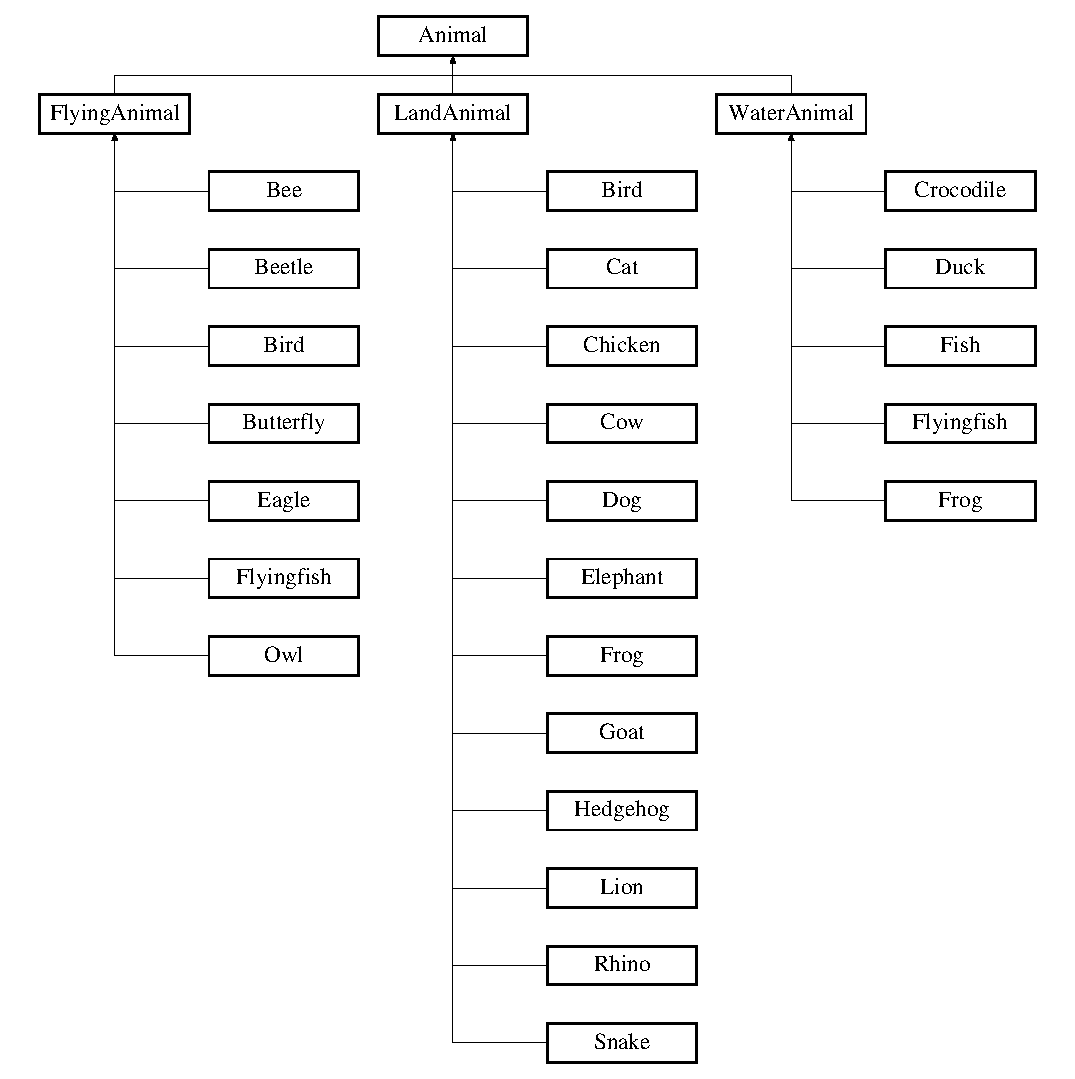
\includegraphics[height=12.000000cm]{classAnimal}
\end{center}
\end{figure}
\subsection*{Public Member Functions}
\begin{DoxyCompactItemize}
\item 
\hypertarget{classAnimal_ae11a2f590886f1772a68a85cc3cacf7c}{{\bfseries Animal} (int, int)}\label{classAnimal_ae11a2f590886f1772a68a85cc3cacf7c}

\item 
\hypertarget{classAnimal_a561ee143993ecb5d83f883dabc42087e}{{\bfseries Animal} (const \hyperlink{classAnimal}{Animal} \&)}\label{classAnimal_a561ee143993ecb5d83f883dabc42087e}

\item 
\hypertarget{classAnimal_a0f89d814c32fd67ce572649f99fab11c}{virtual void {\bfseries set\-X} (int)}\label{classAnimal_a0f89d814c32fd67ce572649f99fab11c}

\item 
\hypertarget{classAnimal_a7a9ee44c7d62feb1207191c5e2c5c34c}{virtual void {\bfseries set\-Y} (int)}\label{classAnimal_a7a9ee44c7d62feb1207191c5e2c5c34c}

\item 
\hypertarget{classAnimal_abf6061a8793776c9be833872ad61e8a3}{virtual int {\bfseries get\-X} ()}\label{classAnimal_abf6061a8793776c9be833872ad61e8a3}

\item 
\hypertarget{classAnimal_a4fcdf96fb0f36aed0ff4eb9f79c7aa11}{virtual int {\bfseries get\-Y} ()}\label{classAnimal_a4fcdf96fb0f36aed0ff4eb9f79c7aa11}

\item 
\hypertarget{classAnimal_aa3fcc58eb4b4f150bf5f9f357e06e7d6}{virtual void {\bfseries add\-Bobot} ()=0}\label{classAnimal_aa3fcc58eb4b4f150bf5f9f357e06e7d6}

\item 
\hypertarget{classAnimal_ada1c15009761c0a85070580f2dd513df}{virtual int {\bfseries get\-Bobot} ()=0}\label{classAnimal_ada1c15009761c0a85070580f2dd513df}

\item 
\hypertarget{classAnimal_ad3baac243ff9d03291a56dd135072472}{virtual char {\bfseries get\-Simbol} ()=0}\label{classAnimal_ad3baac243ff9d03291a56dd135072472}

\item 
\hypertarget{classAnimal_af2d9616bd719adff241a27bd1ba64725}{virtual string {\bfseries interact} ()=0}\label{classAnimal_af2d9616bd719adff241a27bd1ba64725}

\item 
\hypertarget{classAnimal_a0a4dd28bae4de877623c581c4161a5e9}{virtual string {\bfseries get\-Tipe\-Animal} ()=0}\label{classAnimal_a0a4dd28bae4de877623c581c4161a5e9}

\item 
\hypertarget{classAnimal_a3f11826febbaf0b08f3f1f75b2bdc45b}{virtual string {\bfseries get\-Tipe\-Habitat} ()=0}\label{classAnimal_a3f11826febbaf0b08f3f1f75b2bdc45b}

\item 
\hypertarget{classAnimal_a373691a5a672aaf7d2b4fd4dcd8f1288}{virtual string {\bfseries get\-Musuh} (int)=0}\label{classAnimal_a373691a5a672aaf7d2b4fd4dcd8f1288}

\end{DoxyCompactItemize}
\subsection*{Protected Attributes}
\begin{DoxyCompactItemize}
\item 
\hypertarget{classAnimal_a7bf0bfeda35cb1d9737709e9acfb5bfb}{int {\bfseries x}}\label{classAnimal_a7bf0bfeda35cb1d9737709e9acfb5bfb}

\item 
\hypertarget{classAnimal_aecc19a45f1ab7e99a4507938f23a02da}{int {\bfseries y}}\label{classAnimal_aecc19a45f1ab7e99a4507938f23a02da}

\end{DoxyCompactItemize}


The documentation for this class was generated from the following files\-:\begin{DoxyCompactItemize}
\item 
Animal.\-h\item 
Animal.\-cpp\end{DoxyCompactItemize}

\hypertarget{classBee}{\section{Bee Class Reference}
\label{classBee}\index{Bee@{Bee}}
}


{\ttfamily \#include $<$Bee.\-h$>$}

Inheritance diagram for Bee\-:\begin{figure}[H]
\begin{center}
\leavevmode
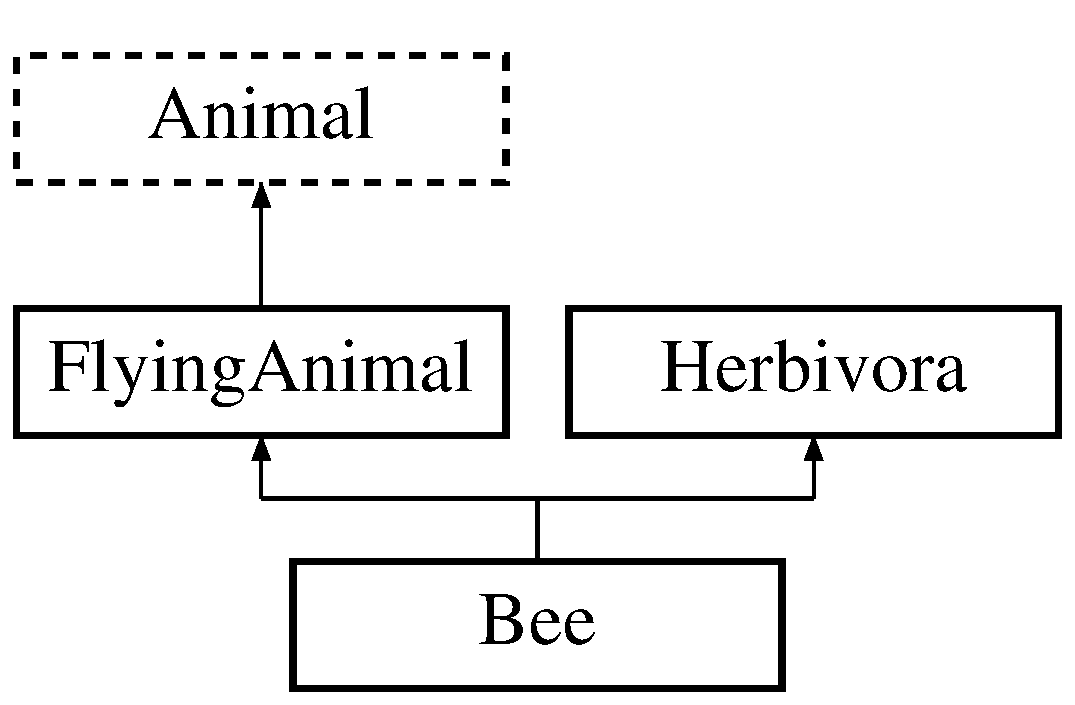
\includegraphics[height=3.000000cm]{classBee}
\end{center}
\end{figure}
\subsection*{Public Member Functions}
\begin{DoxyCompactItemize}
\item 
\hyperlink{classBee_ae8ca9eb389ca41c76bab7058f731abc9}{Bee} (int \-\_\-x, int \-\_\-y)
\begin{DoxyCompactList}\small\item\em Constructor. \end{DoxyCompactList}\item 
\hypertarget{classBee_a769176476ccc499cf45889c3e03baaa2}{\hyperlink{classBee_a769176476ccc499cf45889c3e03baaa2}{$\sim$\-Bee} ()}\label{classBee_a769176476ccc499cf45889c3e03baaa2}

\begin{DoxyCompactList}\small\item\em Destructor. \end{DoxyCompactList}\item 
\hypertarget{classBee_ac13663a9bc08b75dc1120f9e84acc819}{void \hyperlink{classBee_ac13663a9bc08b75dc1120f9e84acc819}{add\-Bobot} ()}\label{classBee_ac13663a9bc08b75dc1120f9e84acc819}

\begin{DoxyCompactList}\small\item\em Menambahkan bobot satu satuan. \end{DoxyCompactList}\item 
int \hyperlink{classBee_a1040d681b2771258e6bcf12c1d4ad19c}{get\-Bobot} ()
\begin{DoxyCompactList}\small\item\em Mendapatkan nilai bobot dari \hyperlink{classBee}{Bee}. \end{DoxyCompactList}\item 
char \hyperlink{classBee_a6e28b4ca1253f48a761f8281a676ed92}{get\-Simbol} ()
\begin{DoxyCompactList}\small\item\em Mendapatkan simbol dari \hyperlink{classBee}{Bee}. \end{DoxyCompactList}\item 
string \hyperlink{classBee_a626c396ba011656c082f7623935c89c9}{get\-Musuh} (int i)
\begin{DoxyCompactList}\small\item\em Mendapatkan musuh ke i dari \hyperlink{classBee}{Bee} Musuh merupakan \hyperlink{classAnimal}{Animal} lain yang tidak bisa tinggal dalam satu kandang dengan \hyperlink{classBee}{Bee}. \end{DoxyCompactList}\item 
string \hyperlink{classBee_ad14bd3aae6bea32bb0a3aaa87d227dc4}{interact} ()
\begin{DoxyCompactList}\small\item\em Mendapatkan reaksi \hyperlink{classBee}{Bee} saat berinteraksi dengan pengunjung. \end{DoxyCompactList}\item 
string \hyperlink{classBee_a0341cf55086556e10104c7744f9fc833}{get\-Tipe\-Animal} ()
\begin{DoxyCompactList}\small\item\em Mendapatkan tipe \hyperlink{classAnimal}{Animal} (nama spesies) \end{DoxyCompactList}\end{DoxyCompactItemize}
\subsection*{Protected Attributes}
\begin{DoxyCompactItemize}
\item 
\hypertarget{classBee_a4b8430bfd71879bf6b80e111bffa396d}{const string {\bfseries tipe\-Animal} = \char`\"{}bee\char`\"{}}\label{classBee_a4b8430bfd71879bf6b80e111bffa396d}

\item 
\hypertarget{classBee_af1c0a138e8e135e49f5ec684fa0d8560}{const char {\bfseries simbol} = 'z'}\label{classBee_af1c0a138e8e135e49f5ec684fa0d8560}

\item 
\hypertarget{classBee_aca646c272b0831555ced51d9d450b2ef}{int {\bfseries bobot}}\label{classBee_aca646c272b0831555ced51d9d450b2ef}

\item 
\hypertarget{classBee_ad03be63a8114e6074f49c3df8dcdf0d3}{string $\ast$ {\bfseries musuh}}\label{classBee_ad03be63a8114e6074f49c3df8dcdf0d3}

\end{DoxyCompactItemize}


\subsection{Detailed Description}
Merupakan \hyperlink{classAnimal}{Animal} yang tinggal di udara dan merupakan \hyperlink{classHerbivora}{Herbivora} 

\subsection{Constructor \& Destructor Documentation}
\hypertarget{classBee_ae8ca9eb389ca41c76bab7058f731abc9}{\index{Bee@{Bee}!Bee@{Bee}}
\index{Bee@{Bee}!Bee@{Bee}}
\subsubsection[{Bee}]{\setlength{\rightskip}{0pt plus 5cm}Bee\-::\-Bee (
\begin{DoxyParamCaption}
\item[{int}]{\-\_\-x, }
\item[{int}]{\-\_\-y}
\end{DoxyParamCaption}
)}}\label{classBee_ae8ca9eb389ca41c76bab7058f731abc9}


Constructor. 


\begin{DoxyParams}{Parameters}
{\em \-\_\-x} & posisi x awal \hyperlink{classBee}{Bee} \\
\hline
{\em \-\_\-y} & posisi y awal \hyperlink{classBee}{Bee} \\
\hline
\end{DoxyParams}


\subsection{Member Function Documentation}
\hypertarget{classBee_a1040d681b2771258e6bcf12c1d4ad19c}{\index{Bee@{Bee}!get\-Bobot@{get\-Bobot}}
\index{get\-Bobot@{get\-Bobot}!Bee@{Bee}}
\subsubsection[{get\-Bobot}]{\setlength{\rightskip}{0pt plus 5cm}int Bee\-::get\-Bobot (
\begin{DoxyParamCaption}
{}
\end{DoxyParamCaption}
)\hspace{0.3cm}{\ttfamily [virtual]}}}\label{classBee_a1040d681b2771258e6bcf12c1d4ad19c}


Mendapatkan nilai bobot dari \hyperlink{classBee}{Bee}. 

\begin{DoxyReturn}{Returns}
bobot 
\end{DoxyReturn}


Implements \hyperlink{classAnimal}{Animal}.

\hypertarget{classBee_a626c396ba011656c082f7623935c89c9}{\index{Bee@{Bee}!get\-Musuh@{get\-Musuh}}
\index{get\-Musuh@{get\-Musuh}!Bee@{Bee}}
\subsubsection[{get\-Musuh}]{\setlength{\rightskip}{0pt plus 5cm}string Bee\-::get\-Musuh (
\begin{DoxyParamCaption}
\item[{int}]{i}
\end{DoxyParamCaption}
)\hspace{0.3cm}{\ttfamily [virtual]}}}\label{classBee_a626c396ba011656c082f7623935c89c9}


Mendapatkan musuh ke i dari \hyperlink{classBee}{Bee} Musuh merupakan \hyperlink{classAnimal}{Animal} lain yang tidak bisa tinggal dalam satu kandang dengan \hyperlink{classBee}{Bee}. 

\begin{DoxyReturn}{Returns}
musuh\mbox{[}i\mbox{]} 
\end{DoxyReturn}


Implements \hyperlink{classAnimal}{Animal}.

\hypertarget{classBee_a6e28b4ca1253f48a761f8281a676ed92}{\index{Bee@{Bee}!get\-Simbol@{get\-Simbol}}
\index{get\-Simbol@{get\-Simbol}!Bee@{Bee}}
\subsubsection[{get\-Simbol}]{\setlength{\rightskip}{0pt plus 5cm}char Bee\-::get\-Simbol (
\begin{DoxyParamCaption}
{}
\end{DoxyParamCaption}
)\hspace{0.3cm}{\ttfamily [virtual]}}}\label{classBee_a6e28b4ca1253f48a761f8281a676ed92}


Mendapatkan simbol dari \hyperlink{classBee}{Bee}. 

\begin{DoxyReturn}{Returns}
simbol 
\end{DoxyReturn}


Implements \hyperlink{classAnimal}{Animal}.

\hypertarget{classBee_a0341cf55086556e10104c7744f9fc833}{\index{Bee@{Bee}!get\-Tipe\-Animal@{get\-Tipe\-Animal}}
\index{get\-Tipe\-Animal@{get\-Tipe\-Animal}!Bee@{Bee}}
\subsubsection[{get\-Tipe\-Animal}]{\setlength{\rightskip}{0pt plus 5cm}string Bee\-::get\-Tipe\-Animal (
\begin{DoxyParamCaption}
{}
\end{DoxyParamCaption}
)\hspace{0.3cm}{\ttfamily [virtual]}}}\label{classBee_a0341cf55086556e10104c7744f9fc833}


Mendapatkan tipe \hyperlink{classAnimal}{Animal} (nama spesies) 

\begin{DoxyReturn}{Returns}
tipe\-Animal 
\end{DoxyReturn}


Implements \hyperlink{classFlyingAnimal_a1523973b9a6a47e9064825c2134fd65d}{Flying\-Animal}.

\hypertarget{classBee_ad14bd3aae6bea32bb0a3aaa87d227dc4}{\index{Bee@{Bee}!interact@{interact}}
\index{interact@{interact}!Bee@{Bee}}
\subsubsection[{interact}]{\setlength{\rightskip}{0pt plus 5cm}string Bee\-::interact (
\begin{DoxyParamCaption}
{}
\end{DoxyParamCaption}
)\hspace{0.3cm}{\ttfamily [virtual]}}}\label{classBee_ad14bd3aae6bea32bb0a3aaa87d227dc4}


Mendapatkan reaksi \hyperlink{classBee}{Bee} saat berinteraksi dengan pengunjung. 

\begin{DoxyReturn}{Returns}
\char`\"{}ngggnggg\char`\"{} 
\end{DoxyReturn}


Implements \hyperlink{classFlyingAnimal_ac0eee625fa2235eee8cbdc0a010ae430}{Flying\-Animal}.



The documentation for this class was generated from the following files\-:\begin{DoxyCompactItemize}
\item 
Bee.\-h\item 
Bee.\-cpp\end{DoxyCompactItemize}

\hypertarget{classBeetle}{\section{Beetle Class Reference}
\label{classBeetle}\index{Beetle@{Beetle}}
}


{\ttfamily \#include $<$Beetle.\-h$>$}

Inheritance diagram for Beetle\-:\begin{figure}[H]
\begin{center}
\leavevmode
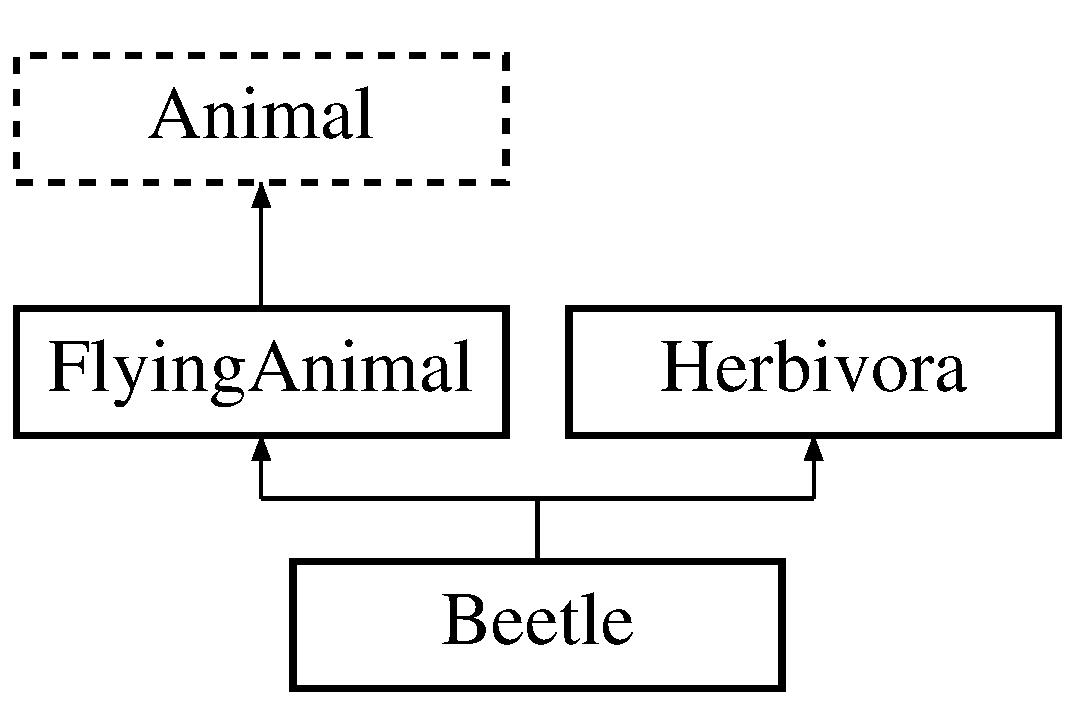
\includegraphics[height=3.000000cm]{classBeetle}
\end{center}
\end{figure}
\subsection*{Public Member Functions}
\begin{DoxyCompactItemize}
\item 
\hyperlink{classBeetle_a44270f6428b6fb3f6fceacce01ecc175}{Beetle} (int \-\_\-x, int \-\_\-y)
\begin{DoxyCompactList}\small\item\em Constructor. \end{DoxyCompactList}\item 
\hypertarget{classBeetle_a49832af20ae5029f08492b5fa1f1f242}{\hyperlink{classBeetle_a49832af20ae5029f08492b5fa1f1f242}{$\sim$\-Beetle} ()}\label{classBeetle_a49832af20ae5029f08492b5fa1f1f242}

\begin{DoxyCompactList}\small\item\em Destructor. \end{DoxyCompactList}\item 
\hypertarget{classBeetle_a1df2c2e5feb89b3619068270d1fbd344}{void \hyperlink{classBeetle_a1df2c2e5feb89b3619068270d1fbd344}{add\-Bobot} ()}\label{classBeetle_a1df2c2e5feb89b3619068270d1fbd344}

\begin{DoxyCompactList}\small\item\em Menambahkan bobot satu satuan. \end{DoxyCompactList}\item 
int \hyperlink{classBeetle_a6c93c4f719178726a355298335923437}{get\-Bobot} ()
\begin{DoxyCompactList}\small\item\em Mendapatkan nilai bobot dari \hyperlink{classBeetle}{Beetle}. \end{DoxyCompactList}\item 
char \hyperlink{classBeetle_a4e47a5dfad4c198a1cc7d4248ca03a35}{get\-Simbol} ()
\begin{DoxyCompactList}\small\item\em Mendapatkan simbol dari \hyperlink{classBeetle}{Beetle}. \end{DoxyCompactList}\item 
string \hyperlink{classBeetle_a3ab31fa3ba09ffdddec91c917bc4779f}{get\-Musuh} (int i)
\begin{DoxyCompactList}\small\item\em Mendapatkan musuh ke i dari \hyperlink{classBeetle}{Beetle} Musuh merupakan \hyperlink{classAnimal}{Animal} lain yang tidak bisa tinggal dalam satu kandang dengan \hyperlink{classBeetle}{Beetle}. \end{DoxyCompactList}\item 
string \hyperlink{classBeetle_a23d1ea3cb62d644a184583f32e6cf102}{interact} ()
\begin{DoxyCompactList}\small\item\em Mendapatkan reaksi \hyperlink{classBeetle}{Beetle} saat berinteraksi dengan pengunjung. \end{DoxyCompactList}\item 
string \hyperlink{classBeetle_a30b538bbf1bf63ca615585bdc512ce33}{get\-Tipe\-Animal} ()
\begin{DoxyCompactList}\small\item\em Mendapatkan tipe \hyperlink{classAnimal}{Animal} (nama spesies) \end{DoxyCompactList}\end{DoxyCompactItemize}
\subsection*{Protected Attributes}
\begin{DoxyCompactItemize}
\item 
\hypertarget{classBeetle_a62b17ee94a6cc5a7188bbd7907d496be}{const string {\bfseries tipe\-Animal} = \char`\"{}beetle\char`\"{}}\label{classBeetle_a62b17ee94a6cc5a7188bbd7907d496be}

\item 
\hypertarget{classBeetle_a25697743a775dcee0c39b6dcf69d87ae}{const char {\bfseries simbol} = 'q'}\label{classBeetle_a25697743a775dcee0c39b6dcf69d87ae}

\item 
\hypertarget{classBeetle_a7541f9cb68d36ec0d694bffd034dffdb}{int {\bfseries bobot}}\label{classBeetle_a7541f9cb68d36ec0d694bffd034dffdb}

\item 
\hypertarget{classBeetle_a2234270060cbd0518c6ccb6df8c7fc33}{string $\ast$ {\bfseries musuh}}\label{classBeetle_a2234270060cbd0518c6ccb6df8c7fc33}

\end{DoxyCompactItemize}


\subsection{Detailed Description}
Merupakan \hyperlink{classAnimal}{Animal} yang tinggal di udara dan merupakan \hyperlink{classHerbivora}{Herbivora} 

\subsection{Constructor \& Destructor Documentation}
\hypertarget{classBeetle_a44270f6428b6fb3f6fceacce01ecc175}{\index{Beetle@{Beetle}!Beetle@{Beetle}}
\index{Beetle@{Beetle}!Beetle@{Beetle}}
\subsubsection[{Beetle}]{\setlength{\rightskip}{0pt plus 5cm}Beetle\-::\-Beetle (
\begin{DoxyParamCaption}
\item[{int}]{\-\_\-x, }
\item[{int}]{\-\_\-y}
\end{DoxyParamCaption}
)}}\label{classBeetle_a44270f6428b6fb3f6fceacce01ecc175}


Constructor. 


\begin{DoxyParams}{Parameters}
{\em \-\_\-x} & posisi x awal \hyperlink{classBeetle}{Beetle} \\
\hline
{\em \-\_\-y} & posisi y awal \hyperlink{classBeetle}{Beetle} \\
\hline
\end{DoxyParams}


\subsection{Member Function Documentation}
\hypertarget{classBeetle_a6c93c4f719178726a355298335923437}{\index{Beetle@{Beetle}!get\-Bobot@{get\-Bobot}}
\index{get\-Bobot@{get\-Bobot}!Beetle@{Beetle}}
\subsubsection[{get\-Bobot}]{\setlength{\rightskip}{0pt plus 5cm}int Beetle\-::get\-Bobot (
\begin{DoxyParamCaption}
{}
\end{DoxyParamCaption}
)\hspace{0.3cm}{\ttfamily [virtual]}}}\label{classBeetle_a6c93c4f719178726a355298335923437}


Mendapatkan nilai bobot dari \hyperlink{classBeetle}{Beetle}. 

\begin{DoxyReturn}{Returns}
bobot 
\end{DoxyReturn}


Implements \hyperlink{classAnimal}{Animal}.

\hypertarget{classBeetle_a3ab31fa3ba09ffdddec91c917bc4779f}{\index{Beetle@{Beetle}!get\-Musuh@{get\-Musuh}}
\index{get\-Musuh@{get\-Musuh}!Beetle@{Beetle}}
\subsubsection[{get\-Musuh}]{\setlength{\rightskip}{0pt plus 5cm}string Beetle\-::get\-Musuh (
\begin{DoxyParamCaption}
\item[{int}]{i}
\end{DoxyParamCaption}
)\hspace{0.3cm}{\ttfamily [virtual]}}}\label{classBeetle_a3ab31fa3ba09ffdddec91c917bc4779f}


Mendapatkan musuh ke i dari \hyperlink{classBeetle}{Beetle} Musuh merupakan \hyperlink{classAnimal}{Animal} lain yang tidak bisa tinggal dalam satu kandang dengan \hyperlink{classBeetle}{Beetle}. 

\begin{DoxyReturn}{Returns}
musuh\mbox{[}i\mbox{]} 
\end{DoxyReturn}


Implements \hyperlink{classAnimal}{Animal}.

\hypertarget{classBeetle_a4e47a5dfad4c198a1cc7d4248ca03a35}{\index{Beetle@{Beetle}!get\-Simbol@{get\-Simbol}}
\index{get\-Simbol@{get\-Simbol}!Beetle@{Beetle}}
\subsubsection[{get\-Simbol}]{\setlength{\rightskip}{0pt plus 5cm}char Beetle\-::get\-Simbol (
\begin{DoxyParamCaption}
{}
\end{DoxyParamCaption}
)\hspace{0.3cm}{\ttfamily [virtual]}}}\label{classBeetle_a4e47a5dfad4c198a1cc7d4248ca03a35}


Mendapatkan simbol dari \hyperlink{classBeetle}{Beetle}. 

\begin{DoxyReturn}{Returns}
simbol 
\end{DoxyReturn}


Implements \hyperlink{classAnimal}{Animal}.

\hypertarget{classBeetle_a30b538bbf1bf63ca615585bdc512ce33}{\index{Beetle@{Beetle}!get\-Tipe\-Animal@{get\-Tipe\-Animal}}
\index{get\-Tipe\-Animal@{get\-Tipe\-Animal}!Beetle@{Beetle}}
\subsubsection[{get\-Tipe\-Animal}]{\setlength{\rightskip}{0pt plus 5cm}string Beetle\-::get\-Tipe\-Animal (
\begin{DoxyParamCaption}
{}
\end{DoxyParamCaption}
)\hspace{0.3cm}{\ttfamily [virtual]}}}\label{classBeetle_a30b538bbf1bf63ca615585bdc512ce33}


Mendapatkan tipe \hyperlink{classAnimal}{Animal} (nama spesies) 

\begin{DoxyReturn}{Returns}
tipe\-Animal 
\end{DoxyReturn}


Implements \hyperlink{classFlyingAnimal_a1523973b9a6a47e9064825c2134fd65d}{Flying\-Animal}.

\hypertarget{classBeetle_a23d1ea3cb62d644a184583f32e6cf102}{\index{Beetle@{Beetle}!interact@{interact}}
\index{interact@{interact}!Beetle@{Beetle}}
\subsubsection[{interact}]{\setlength{\rightskip}{0pt plus 5cm}string Beetle\-::interact (
\begin{DoxyParamCaption}
{}
\end{DoxyParamCaption}
)\hspace{0.3cm}{\ttfamily [virtual]}}}\label{classBeetle_a23d1ea3cb62d644a184583f32e6cf102}


Mendapatkan reaksi \hyperlink{classBeetle}{Beetle} saat berinteraksi dengan pengunjung. 

\begin{DoxyReturn}{Returns}
\char`\"{}kepakkepak\char`\"{} 
\end{DoxyReturn}


Implements \hyperlink{classFlyingAnimal_ac0eee625fa2235eee8cbdc0a010ae430}{Flying\-Animal}.



The documentation for this class was generated from the following files\-:\begin{DoxyCompactItemize}
\item 
Beetle.\-h\item 
Beetle.\-cpp\end{DoxyCompactItemize}

\hypertarget{classBird}{\section{Bird Class Reference}
\label{classBird}\index{Bird@{Bird}}
}


{\ttfamily \#include $<$Bird.\-h$>$}

Inheritance diagram for Bird\-:\begin{figure}[H]
\begin{center}
\leavevmode
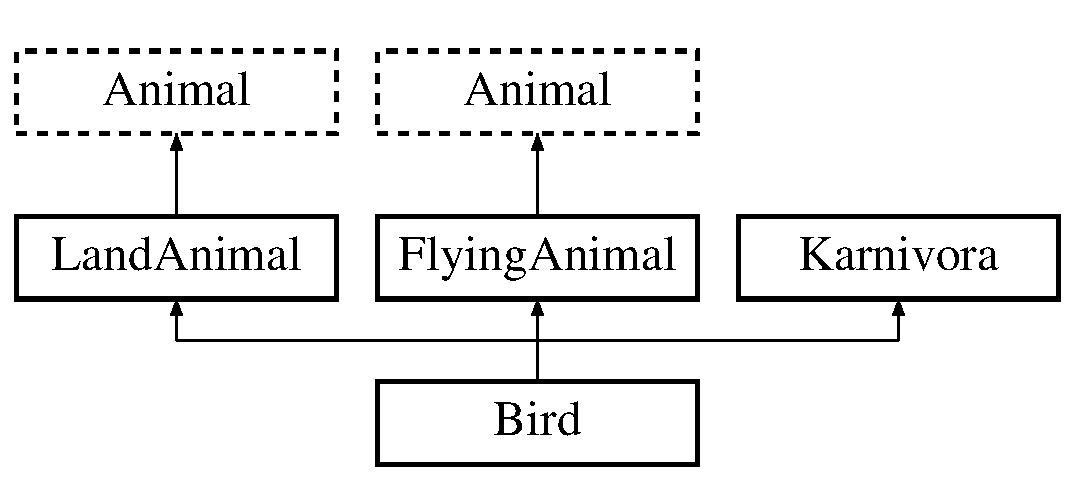
\includegraphics[height=3.000000cm]{classBird}
\end{center}
\end{figure}
\subsection*{Public Member Functions}
\begin{DoxyCompactItemize}
\item 
\hyperlink{classBird_a802e609916df32347f8b2d535647c232}{Bird} (int \-\_\-x, int \-\_\-y)
\begin{DoxyCompactList}\small\item\em Constructor. \end{DoxyCompactList}\item 
\hypertarget{classBird_a7d10693b91a2736611c37f1ef205b911}{\hyperlink{classBird_a7d10693b91a2736611c37f1ef205b911}{$\sim$\-Bird} ()}\label{classBird_a7d10693b91a2736611c37f1ef205b911}

\begin{DoxyCompactList}\small\item\em Destructor. \end{DoxyCompactList}\item 
\hypertarget{classBird_a43377def001a07e9a94f15559f82abd3}{void \hyperlink{classBird_a43377def001a07e9a94f15559f82abd3}{add\-Bobot} ()}\label{classBird_a43377def001a07e9a94f15559f82abd3}

\begin{DoxyCompactList}\small\item\em Menambahkan bobot satu satuan. \end{DoxyCompactList}\item 
int \hyperlink{classBird_a72a377b7d210dc3cabd57d61538eeeac}{get\-Bobot} ()
\begin{DoxyCompactList}\small\item\em Mendapatkan nilai bobot dari \hyperlink{classBird}{Bird}. \end{DoxyCompactList}\item 
char \hyperlink{classBird_a842d9c5760dd027cc293b869b7a5c9f7}{get\-Simbol} ()
\begin{DoxyCompactList}\small\item\em Mendapatkan simbol dari \hyperlink{classBird}{Bird}. \end{DoxyCompactList}\item 
string \hyperlink{classBird_a957350fef42a0a16446abfd9a14a8f07}{get\-Musuh} (int i)
\begin{DoxyCompactList}\small\item\em Mendapatkan musuh ke i dari \hyperlink{classBird}{Bird} Musuh merupakan \hyperlink{classAnimal}{Animal} lain yang tidak bisa tinggal dalam satu kandang dengan \hyperlink{classBird}{Bird}. \end{DoxyCompactList}\item 
string \hyperlink{classBird_ae1e5a507154e6aeb2ba9f3c8447c75d4}{interact} ()
\begin{DoxyCompactList}\small\item\em Mendapatkan reaksi \hyperlink{classBird}{Bird} saat berinteraksi dengan pengunjung. \end{DoxyCompactList}\item 
string \hyperlink{classBird_a334d9a9e90114f5c74d2ad327120b2be}{get\-Tipe\-Animal} ()
\begin{DoxyCompactList}\small\item\em Mendapatkan tipe \hyperlink{classAnimal}{Animal} (nama spesies) \end{DoxyCompactList}\end{DoxyCompactItemize}
\subsection*{Protected Attributes}
\begin{DoxyCompactItemize}
\item 
\hypertarget{classBird_a38f99d6857557f22110704917b8a9164}{const string {\bfseries tipe\-Animal} = \char`\"{}bird\char`\"{}}\label{classBird_a38f99d6857557f22110704917b8a9164}

\item 
\hypertarget{classBird_a70b1f7bc29b88c9f23082179a1aa3ab4}{const char {\bfseries simbol} = 'b'}\label{classBird_a70b1f7bc29b88c9f23082179a1aa3ab4}

\item 
\hypertarget{classBird_adb9c2c0a72dec783172ebc73ca6a8a0a}{int {\bfseries bobot}}\label{classBird_adb9c2c0a72dec783172ebc73ca6a8a0a}

\item 
\hypertarget{classBird_a21567839a88ed9e9d9124e16ced21a5d}{string $\ast$ {\bfseries musuh}}\label{classBird_a21567839a88ed9e9d9124e16ced21a5d}

\end{DoxyCompactItemize}


\subsection{Detailed Description}
Merupakan \hyperlink{classAnimal}{Animal} yang tinggal di darat dan merupakan \hyperlink{classKarnivora}{Karnivora} 

\subsection{Constructor \& Destructor Documentation}
\hypertarget{classBird_a802e609916df32347f8b2d535647c232}{\index{Bird@{Bird}!Bird@{Bird}}
\index{Bird@{Bird}!Bird@{Bird}}
\subsubsection[{Bird}]{\setlength{\rightskip}{0pt plus 5cm}Bird\-::\-Bird (
\begin{DoxyParamCaption}
\item[{int}]{\-\_\-x, }
\item[{int}]{\-\_\-y}
\end{DoxyParamCaption}
)}}\label{classBird_a802e609916df32347f8b2d535647c232}


Constructor. 


\begin{DoxyParams}{Parameters}
{\em \-\_\-x} & posisi x awal \hyperlink{classBird}{Bird} \\
\hline
{\em \-\_\-y} & posisi y awal \hyperlink{classBird}{Bird} \\
\hline
\end{DoxyParams}


\subsection{Member Function Documentation}
\hypertarget{classBird_a72a377b7d210dc3cabd57d61538eeeac}{\index{Bird@{Bird}!get\-Bobot@{get\-Bobot}}
\index{get\-Bobot@{get\-Bobot}!Bird@{Bird}}
\subsubsection[{get\-Bobot}]{\setlength{\rightskip}{0pt plus 5cm}int Bird\-::get\-Bobot (
\begin{DoxyParamCaption}
{}
\end{DoxyParamCaption}
)\hspace{0.3cm}{\ttfamily [virtual]}}}\label{classBird_a72a377b7d210dc3cabd57d61538eeeac}


Mendapatkan nilai bobot dari \hyperlink{classBird}{Bird}. 

\begin{DoxyReturn}{Returns}
bobot 
\end{DoxyReturn}


Implements \hyperlink{classAnimal}{Animal}.

\hypertarget{classBird_a957350fef42a0a16446abfd9a14a8f07}{\index{Bird@{Bird}!get\-Musuh@{get\-Musuh}}
\index{get\-Musuh@{get\-Musuh}!Bird@{Bird}}
\subsubsection[{get\-Musuh}]{\setlength{\rightskip}{0pt plus 5cm}string Bird\-::get\-Musuh (
\begin{DoxyParamCaption}
\item[{int}]{i}
\end{DoxyParamCaption}
)\hspace{0.3cm}{\ttfamily [virtual]}}}\label{classBird_a957350fef42a0a16446abfd9a14a8f07}


Mendapatkan musuh ke i dari \hyperlink{classBird}{Bird} Musuh merupakan \hyperlink{classAnimal}{Animal} lain yang tidak bisa tinggal dalam satu kandang dengan \hyperlink{classBird}{Bird}. 

\begin{DoxyReturn}{Returns}
musuh\mbox{[}i\mbox{]} 
\end{DoxyReturn}


Implements \hyperlink{classAnimal}{Animal}.

\hypertarget{classBird_a842d9c5760dd027cc293b869b7a5c9f7}{\index{Bird@{Bird}!get\-Simbol@{get\-Simbol}}
\index{get\-Simbol@{get\-Simbol}!Bird@{Bird}}
\subsubsection[{get\-Simbol}]{\setlength{\rightskip}{0pt plus 5cm}char Bird\-::get\-Simbol (
\begin{DoxyParamCaption}
{}
\end{DoxyParamCaption}
)\hspace{0.3cm}{\ttfamily [virtual]}}}\label{classBird_a842d9c5760dd027cc293b869b7a5c9f7}


Mendapatkan simbol dari \hyperlink{classBird}{Bird}. 

\begin{DoxyReturn}{Returns}
simbol 
\end{DoxyReturn}


Implements \hyperlink{classAnimal}{Animal}.

\hypertarget{classBird_a334d9a9e90114f5c74d2ad327120b2be}{\index{Bird@{Bird}!get\-Tipe\-Animal@{get\-Tipe\-Animal}}
\index{get\-Tipe\-Animal@{get\-Tipe\-Animal}!Bird@{Bird}}
\subsubsection[{get\-Tipe\-Animal}]{\setlength{\rightskip}{0pt plus 5cm}string Bird\-::get\-Tipe\-Animal (
\begin{DoxyParamCaption}
{}
\end{DoxyParamCaption}
)\hspace{0.3cm}{\ttfamily [virtual]}}}\label{classBird_a334d9a9e90114f5c74d2ad327120b2be}


Mendapatkan tipe \hyperlink{classAnimal}{Animal} (nama spesies) 

\begin{DoxyReturn}{Returns}
tipe\-Animal 
\end{DoxyReturn}


Implements \hyperlink{classFlyingAnimal_a1523973b9a6a47e9064825c2134fd65d}{Flying\-Animal}.

\hypertarget{classBird_ae1e5a507154e6aeb2ba9f3c8447c75d4}{\index{Bird@{Bird}!interact@{interact}}
\index{interact@{interact}!Bird@{Bird}}
\subsubsection[{interact}]{\setlength{\rightskip}{0pt plus 5cm}string Bird\-::interact (
\begin{DoxyParamCaption}
{}
\end{DoxyParamCaption}
)\hspace{0.3cm}{\ttfamily [virtual]}}}\label{classBird_ae1e5a507154e6aeb2ba9f3c8447c75d4}


Mendapatkan reaksi \hyperlink{classBird}{Bird} saat berinteraksi dengan pengunjung. 

\begin{DoxyReturn}{Returns}
\char`\"{}cuitcuit\char`\"{} 
\end{DoxyReturn}


Implements \hyperlink{classFlyingAnimal_ac0eee625fa2235eee8cbdc0a010ae430}{Flying\-Animal}.



The documentation for this class was generated from the following files\-:\begin{DoxyCompactItemize}
\item 
Bird.\-h\item 
Bird.\-cpp\end{DoxyCompactItemize}

\hypertarget{classButterfly}{\section{Butterfly Class Reference}
\label{classButterfly}\index{Butterfly@{Butterfly}}
}


{\ttfamily \#include $<$Butterfly.\-h$>$}

Inheritance diagram for Butterfly\-:\begin{figure}[H]
\begin{center}
\leavevmode
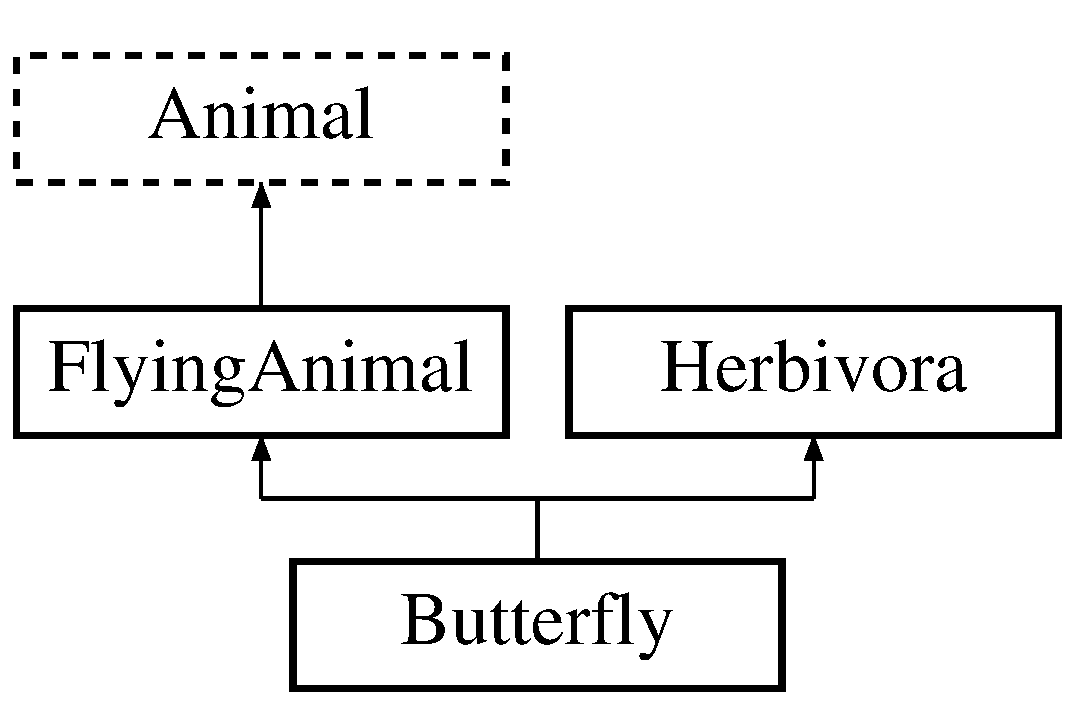
\includegraphics[height=3.000000cm]{classButterfly}
\end{center}
\end{figure}
\subsection*{Public Member Functions}
\begin{DoxyCompactItemize}
\item 
\hyperlink{classButterfly_aad74a900dcfae28b2f481e86148d6fad}{Butterfly} (int \-\_\-x, int \-\_\-y)
\begin{DoxyCompactList}\small\item\em Constructor. \end{DoxyCompactList}\item 
\hypertarget{classButterfly_aa6e58d14c62f35e6b4d8a84d4396d30e}{\hyperlink{classButterfly_aa6e58d14c62f35e6b4d8a84d4396d30e}{$\sim$\-Butterfly} ()}\label{classButterfly_aa6e58d14c62f35e6b4d8a84d4396d30e}

\begin{DoxyCompactList}\small\item\em Destructor. \end{DoxyCompactList}\item 
\hypertarget{classButterfly_ad1458d18e99f90979f20123cda50b6b3}{void \hyperlink{classButterfly_ad1458d18e99f90979f20123cda50b6b3}{add\-Bobot} ()}\label{classButterfly_ad1458d18e99f90979f20123cda50b6b3}

\begin{DoxyCompactList}\small\item\em Menambahkan bobot satu satuan. \end{DoxyCompactList}\item 
int \hyperlink{classButterfly_ac802d3934d533606ee8c4229265d0be1}{get\-Bobot} ()
\begin{DoxyCompactList}\small\item\em Mendapatkan nilai bobot dari \hyperlink{classButterfly}{Butterfly}. \end{DoxyCompactList}\item 
char \hyperlink{classButterfly_a15c3ae75ea826f50d25bb347abe4a4c4}{get\-Simbol} ()
\begin{DoxyCompactList}\small\item\em Mendapatkan simbol dari \hyperlink{classButterfly}{Butterfly}. \end{DoxyCompactList}\item 
string \hyperlink{classButterfly_a42116546aa9eb5dd2cac11761cfe749e}{get\-Musuh} (int i)
\begin{DoxyCompactList}\small\item\em Mendapatkan musuh ke i dari \hyperlink{classButterfly}{Butterfly} Musuh merupakan \hyperlink{classAnimal}{Animal} lain yang tidak bisa tinggal dalam satu kandang dengan \hyperlink{classButterfly}{Butterfly}. \end{DoxyCompactList}\item 
string \hyperlink{classButterfly_a64595ce265c79591af2095880bca70f1}{interact} ()
\begin{DoxyCompactList}\small\item\em Mendapatkan reaksi \hyperlink{classButterfly}{Butterfly} saat berinteraksi dengan pengunjung. \end{DoxyCompactList}\item 
string \hyperlink{classButterfly_a7a11185ad98c664b3d3f052336afec0e}{get\-Tipe\-Animal} ()
\begin{DoxyCompactList}\small\item\em Mendapatkan tipe \hyperlink{classAnimal}{Animal} (nama spesies) \end{DoxyCompactList}\end{DoxyCompactItemize}
\subsection*{Protected Attributes}
\begin{DoxyCompactItemize}
\item 
\hypertarget{classButterfly_a1eed2cdb5d97914a6cf5f523d650247b}{const string {\bfseries tipe\-Animal} = \char`\"{}butterfly\char`\"{}}\label{classButterfly_a1eed2cdb5d97914a6cf5f523d650247b}

\item 
\hypertarget{classButterfly_aca91bfe3883f3c8d580aafcb5f88598a}{const char {\bfseries simbol} = 't'}\label{classButterfly_aca91bfe3883f3c8d580aafcb5f88598a}

\item 
\hypertarget{classButterfly_a5ba39cb122e32cfdf5946639737389e7}{int {\bfseries bobot}}\label{classButterfly_a5ba39cb122e32cfdf5946639737389e7}

\item 
\hypertarget{classButterfly_ac90041697ff547883bb1a4398c473c68}{string $\ast$ {\bfseries musuh}}\label{classButterfly_ac90041697ff547883bb1a4398c473c68}

\end{DoxyCompactItemize}


\subsection{Detailed Description}
Merupakan \hyperlink{classAnimal}{Animal} yang tinggal di udara dan merupakan \hyperlink{classHerbivora}{Herbivora} 

\subsection{Constructor \& Destructor Documentation}
\hypertarget{classButterfly_aad74a900dcfae28b2f481e86148d6fad}{\index{Butterfly@{Butterfly}!Butterfly@{Butterfly}}
\index{Butterfly@{Butterfly}!Butterfly@{Butterfly}}
\subsubsection[{Butterfly}]{\setlength{\rightskip}{0pt plus 5cm}Butterfly\-::\-Butterfly (
\begin{DoxyParamCaption}
\item[{int}]{\-\_\-x, }
\item[{int}]{\-\_\-y}
\end{DoxyParamCaption}
)}}\label{classButterfly_aad74a900dcfae28b2f481e86148d6fad}


Constructor. 


\begin{DoxyParams}{Parameters}
{\em \-\_\-x} & posisi x awal \hyperlink{classButterfly}{Butterfly} \\
\hline
{\em \-\_\-y} & posisi y awal \hyperlink{classButterfly}{Butterfly} \\
\hline
\end{DoxyParams}


\subsection{Member Function Documentation}
\hypertarget{classButterfly_ac802d3934d533606ee8c4229265d0be1}{\index{Butterfly@{Butterfly}!get\-Bobot@{get\-Bobot}}
\index{get\-Bobot@{get\-Bobot}!Butterfly@{Butterfly}}
\subsubsection[{get\-Bobot}]{\setlength{\rightskip}{0pt plus 5cm}int Butterfly\-::get\-Bobot (
\begin{DoxyParamCaption}
{}
\end{DoxyParamCaption}
)\hspace{0.3cm}{\ttfamily [virtual]}}}\label{classButterfly_ac802d3934d533606ee8c4229265d0be1}


Mendapatkan nilai bobot dari \hyperlink{classButterfly}{Butterfly}. 

\begin{DoxyReturn}{Returns}
bobot 
\end{DoxyReturn}


Implements \hyperlink{classAnimal}{Animal}.

\hypertarget{classButterfly_a42116546aa9eb5dd2cac11761cfe749e}{\index{Butterfly@{Butterfly}!get\-Musuh@{get\-Musuh}}
\index{get\-Musuh@{get\-Musuh}!Butterfly@{Butterfly}}
\subsubsection[{get\-Musuh}]{\setlength{\rightskip}{0pt plus 5cm}string Butterfly\-::get\-Musuh (
\begin{DoxyParamCaption}
\item[{int}]{i}
\end{DoxyParamCaption}
)\hspace{0.3cm}{\ttfamily [virtual]}}}\label{classButterfly_a42116546aa9eb5dd2cac11761cfe749e}


Mendapatkan musuh ke i dari \hyperlink{classButterfly}{Butterfly} Musuh merupakan \hyperlink{classAnimal}{Animal} lain yang tidak bisa tinggal dalam satu kandang dengan \hyperlink{classButterfly}{Butterfly}. 

\begin{DoxyReturn}{Returns}
musuh\mbox{[}i\mbox{]} 
\end{DoxyReturn}


Implements \hyperlink{classAnimal}{Animal}.

\hypertarget{classButterfly_a15c3ae75ea826f50d25bb347abe4a4c4}{\index{Butterfly@{Butterfly}!get\-Simbol@{get\-Simbol}}
\index{get\-Simbol@{get\-Simbol}!Butterfly@{Butterfly}}
\subsubsection[{get\-Simbol}]{\setlength{\rightskip}{0pt plus 5cm}char Butterfly\-::get\-Simbol (
\begin{DoxyParamCaption}
{}
\end{DoxyParamCaption}
)\hspace{0.3cm}{\ttfamily [virtual]}}}\label{classButterfly_a15c3ae75ea826f50d25bb347abe4a4c4}


Mendapatkan simbol dari \hyperlink{classButterfly}{Butterfly}. 

\begin{DoxyReturn}{Returns}
simbol 
\end{DoxyReturn}


Implements \hyperlink{classAnimal}{Animal}.

\hypertarget{classButterfly_a7a11185ad98c664b3d3f052336afec0e}{\index{Butterfly@{Butterfly}!get\-Tipe\-Animal@{get\-Tipe\-Animal}}
\index{get\-Tipe\-Animal@{get\-Tipe\-Animal}!Butterfly@{Butterfly}}
\subsubsection[{get\-Tipe\-Animal}]{\setlength{\rightskip}{0pt plus 5cm}string Butterfly\-::get\-Tipe\-Animal (
\begin{DoxyParamCaption}
{}
\end{DoxyParamCaption}
)\hspace{0.3cm}{\ttfamily [virtual]}}}\label{classButterfly_a7a11185ad98c664b3d3f052336afec0e}


Mendapatkan tipe \hyperlink{classAnimal}{Animal} (nama spesies) 

\begin{DoxyReturn}{Returns}
tipe\-Animal 
\end{DoxyReturn}


Implements \hyperlink{classFlyingAnimal_a1523973b9a6a47e9064825c2134fd65d}{Flying\-Animal}.

\hypertarget{classButterfly_a64595ce265c79591af2095880bca70f1}{\index{Butterfly@{Butterfly}!interact@{interact}}
\index{interact@{interact}!Butterfly@{Butterfly}}
\subsubsection[{interact}]{\setlength{\rightskip}{0pt plus 5cm}string Butterfly\-::interact (
\begin{DoxyParamCaption}
{}
\end{DoxyParamCaption}
)\hspace{0.3cm}{\ttfamily [virtual]}}}\label{classButterfly_a64595ce265c79591af2095880bca70f1}


Mendapatkan reaksi \hyperlink{classButterfly}{Butterfly} saat berinteraksi dengan pengunjung. 

\begin{DoxyReturn}{Returns}
\char`\"{}flyfly\char`\"{} 
\end{DoxyReturn}


Implements \hyperlink{classFlyingAnimal_ac0eee625fa2235eee8cbdc0a010ae430}{Flying\-Animal}.



The documentation for this class was generated from the following files\-:\begin{DoxyCompactItemize}
\item 
Butterfly.\-h\item 
Butterfly.\-cpp\end{DoxyCompactItemize}

\hypertarget{classCage}{\section{Cage Class Reference}
\label{classCage}\index{Cage@{Cage}}
}


{\ttfamily \#include $<$Cage.\-h$>$}

Inheritance diagram for Cage\-:\begin{figure}[H]
\begin{center}
\leavevmode
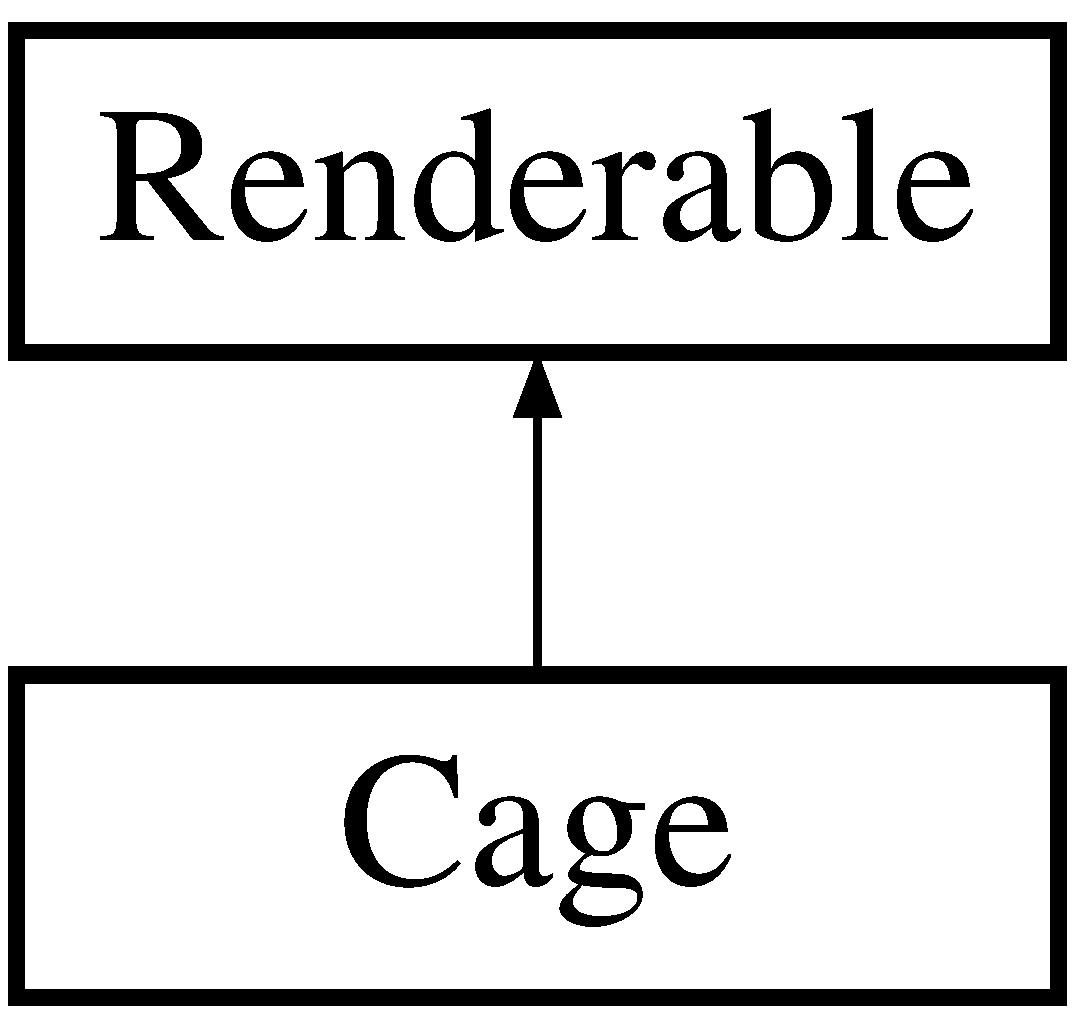
\includegraphics[height=2.000000cm]{classCage}
\end{center}
\end{figure}
\subsection*{Public Member Functions}
\begin{DoxyCompactItemize}
\item 
\hyperlink{classCage_adf3c087a1f7526422db7ce5e37469c91}{Cage} (char simbol, string tipe\-Habitat)
\begin{DoxyCompactList}\small\item\em Constructor Membangun cage. \end{DoxyCompactList}\item 
\hypertarget{classCage_a657259499dfc23c63fc65aeaf8abbb17}{\hyperlink{classCage_a657259499dfc23c63fc65aeaf8abbb17}{$\sim$\-Cage} ()}\label{classCage_a657259499dfc23c63fc65aeaf8abbb17}

\begin{DoxyCompactList}\small\item\em Destructor. \end{DoxyCompactList}\item 
int \hyperlink{classCage_a095e180cfe3c617f14ba102cb1c99f07}{get\-Cage\-Area} ()
\begin{DoxyCompactList}\small\item\em Getter cage\-Area. Mendapatkan banyak petak maksimal yang dapat dibangun. \end{DoxyCompactList}\item 
int \hyperlink{classCage_a782080ce97d84f0ddfdc46f4c11e1cdf}{get\-N\-Area} ()
\begin{DoxyCompactList}\small\item\em Getter n\-Area. Mendapatkan jumlah petak yang telah dibangun. \end{DoxyCompactList}\item 
int \hyperlink{classCage_af67deefc75632b3d13007cb5f06109b8}{get\-N\-Animal} ()
\begin{DoxyCompactList}\small\item\em Getter n\-Animal. Mendapatkan jumlah \hyperlink{classAnimal}{Animal} yang terdapat pada cage. \end{DoxyCompactList}\item 
string \hyperlink{classCage_a762b5f166b260fadf7b6fd21e231c02b}{get\-Tipe\-Habitat} ()
\begin{DoxyCompactList}\small\item\em Getter tipe\-Habitat Mendapatkan tipe habitat \hyperlink{classCage}{Cage}. \end{DoxyCompactList}\item 
\hyperlink{classCell}{Cell} $\ast$ \hyperlink{classCage_a501c11daaeee7968a477412ec00c140e}{get\-Cage\-Position} (int i)
\begin{DoxyCompactList}\small\item\em Getter \hyperlink{classCage}{Cage} Position Mendapatkan list\-Of\-Cage\-Position\mbox{[}i\mbox{]}. \end{DoxyCompactList}\item 
\hyperlink{classAnimal}{Animal} $\ast$ \hyperlink{classCage_aa3e42c058261cdc8da4479afe1342dc7}{get\-Animal} (int i)
\begin{DoxyCompactList}\small\item\em Getter \hyperlink{classAnimal}{Animal} Mendapatkan \hyperlink{classAnimal}{Animal} pada indeks i (animals\mbox{[}i\mbox{]}) \end{DoxyCompactList}\item 
int \hyperlink{classCage_ade3f9a83cbceecbc2f8b2d239d00ac7a}{get\-Max\-Animal} ()
\begin{DoxyCompactList}\small\item\em max animal Maksimal animal dalam cage = 30\% dari cage\-Area \end{DoxyCompactList}\item 
int \hyperlink{classCage_a5e5df3e1f60eb1e0577e11f12e73a659}{get\-Total\-Makanan} ()
\begin{DoxyCompactList}\small\item\em Mengembalikan total makanan yang diperlukan \hyperlink{classAnimal}{Animal} dalam satu \hyperlink{classCage}{Cage}. \end{DoxyCompactList}\item 
void \hyperlink{classCage_a45bf1594e9f1c25a7f85f08a2cab162f}{add\-Cage\-Position} (\hyperlink{classCell}{Cell} $\ast$position)
\begin{DoxyCompactList}\small\item\em Setter list\-Of\-Cage\-Position. Menambahkan posisi cell tempat didirikannya cage. \end{DoxyCompactList}\item 
void \hyperlink{classCage_ab2be8c3b1027d620ee0dbedbb9e5637d}{add\-Animal} (\hyperlink{classAnimal}{Animal} $\ast$anim)
\begin{DoxyCompactList}\small\item\em Setter animals. Menambahkan \hyperlink{classAnimal}{Animal} dalam cage jika masih bisa ditambahkan. Harus dipastikan jumlah \hyperlink{classAnimal}{Animal} tidak melebihi kapasitasnya. \end{DoxyCompactList}\item 
bool \hyperlink{classCage_adf86b9bd1da9aa59bf403320060bd455}{is\-Position\-Empty} (\hyperlink{classCell}{Cell} $\ast$c)
\begin{DoxyCompactList}\small\item\em Menentukan apakah suatu cell cage telah ditempati animal atau belum. \end{DoxyCompactList}\item 
bool \hyperlink{classCage_a72166ea7b4a83b59f54131b354272154}{is\-Position\-In\-Cage} (int x, int y)
\begin{DoxyCompactList}\small\item\em Menentukan apakah posisi (x,y) terdapat di salah satu posisi cage dibangun. \end{DoxyCompactList}\item 
char \hyperlink{classCage_aab864d541ada79ac83619b139bef5507}{render} ()
\begin{DoxyCompactList}\small\item\em getter S\-I\-M\-B\-O\-L Mengembalikan nilai S\-I\-M\-B\-O\-L \end{DoxyCompactList}\end{DoxyCompactItemize}


\subsection{Detailed Description}
Merupakan \hyperlink{classCage}{Cage} yang terdiri dari beberapa petak \hyperlink{classCell}{Cell} pada habitat tertentu. 

\subsection{Constructor \& Destructor Documentation}
\hypertarget{classCage_adf3c087a1f7526422db7ce5e37469c91}{\index{Cage@{Cage}!Cage@{Cage}}
\index{Cage@{Cage}!Cage@{Cage}}
\subsubsection[{Cage}]{\setlength{\rightskip}{0pt plus 5cm}Cage\-::\-Cage (
\begin{DoxyParamCaption}
\item[{char}]{simbol, }
\item[{string}]{tipe\-Habitat}
\end{DoxyParamCaption}
)}}\label{classCage_adf3c087a1f7526422db7ce5e37469c91}


Constructor Membangun cage. 


\begin{DoxyParams}{Parameters}
{\em simbol} & Simbol dari cage \\
\hline
{\em tipehabitat} & Tipe habitat cage \\
\hline
{\em cage\-Area} & Luas cage / jumlah cell \\
\hline
\end{DoxyParams}


\subsection{Member Function Documentation}
\hypertarget{classCage_ab2be8c3b1027d620ee0dbedbb9e5637d}{\index{Cage@{Cage}!add\-Animal@{add\-Animal}}
\index{add\-Animal@{add\-Animal}!Cage@{Cage}}
\subsubsection[{add\-Animal}]{\setlength{\rightskip}{0pt plus 5cm}void Cage\-::add\-Animal (
\begin{DoxyParamCaption}
\item[{{\bf Animal} $\ast$}]{anim}
\end{DoxyParamCaption}
)}}\label{classCage_ab2be8c3b1027d620ee0dbedbb9e5637d}


Setter animals. Menambahkan \hyperlink{classAnimal}{Animal} dalam cage jika masih bisa ditambahkan. Harus dipastikan jumlah \hyperlink{classAnimal}{Animal} tidak melebihi kapasitasnya. 


\begin{DoxyParams}{Parameters}
{\em anim} & \hyperlink{classAnimal}{Animal} yang akan ditambahkan \\
\hline
\end{DoxyParams}
\hypertarget{classCage_a45bf1594e9f1c25a7f85f08a2cab162f}{\index{Cage@{Cage}!add\-Cage\-Position@{add\-Cage\-Position}}
\index{add\-Cage\-Position@{add\-Cage\-Position}!Cage@{Cage}}
\subsubsection[{add\-Cage\-Position}]{\setlength{\rightskip}{0pt plus 5cm}void Cage\-::add\-Cage\-Position (
\begin{DoxyParamCaption}
\item[{{\bf Cell} $\ast$}]{position}
\end{DoxyParamCaption}
)}}\label{classCage_a45bf1594e9f1c25a7f85f08a2cab162f}


Setter list\-Of\-Cage\-Position. Menambahkan posisi cell tempat didirikannya cage. 


\begin{DoxyParams}{Parameters}
{\em position} & Posisi cage \\
\hline
\end{DoxyParams}
\hypertarget{classCage_aa3e42c058261cdc8da4479afe1342dc7}{\index{Cage@{Cage}!get\-Animal@{get\-Animal}}
\index{get\-Animal@{get\-Animal}!Cage@{Cage}}
\subsubsection[{get\-Animal}]{\setlength{\rightskip}{0pt plus 5cm}{\bf Animal} $\ast$ Cage\-::get\-Animal (
\begin{DoxyParamCaption}
\item[{int}]{i}
\end{DoxyParamCaption}
)}}\label{classCage_aa3e42c058261cdc8da4479afe1342dc7}


Getter \hyperlink{classAnimal}{Animal} Mendapatkan \hyperlink{classAnimal}{Animal} pada indeks i (animals\mbox{[}i\mbox{]}) 


\begin{DoxyParams}{Parameters}
{\em i} & Index \hyperlink{classAnimal}{Animal} yang akan diambil \\
\hline
\end{DoxyParams}
\begin{DoxyReturn}{Returns}
animals\mbox{[}i\mbox{]} 
\end{DoxyReturn}
\hypertarget{classCage_a095e180cfe3c617f14ba102cb1c99f07}{\index{Cage@{Cage}!get\-Cage\-Area@{get\-Cage\-Area}}
\index{get\-Cage\-Area@{get\-Cage\-Area}!Cage@{Cage}}
\subsubsection[{get\-Cage\-Area}]{\setlength{\rightskip}{0pt plus 5cm}int Cage\-::get\-Cage\-Area (
\begin{DoxyParamCaption}
{}
\end{DoxyParamCaption}
)}}\label{classCage_a095e180cfe3c617f14ba102cb1c99f07}


Getter cage\-Area. Mendapatkan banyak petak maksimal yang dapat dibangun. 

\begin{DoxyReturn}{Returns}
cage\-Area 
\end{DoxyReturn}
\hypertarget{classCage_a501c11daaeee7968a477412ec00c140e}{\index{Cage@{Cage}!get\-Cage\-Position@{get\-Cage\-Position}}
\index{get\-Cage\-Position@{get\-Cage\-Position}!Cage@{Cage}}
\subsubsection[{get\-Cage\-Position}]{\setlength{\rightskip}{0pt plus 5cm}{\bf Cell} $\ast$ Cage\-::get\-Cage\-Position (
\begin{DoxyParamCaption}
\item[{int}]{i}
\end{DoxyParamCaption}
)}}\label{classCage_a501c11daaeee7968a477412ec00c140e}


Getter \hyperlink{classCage}{Cage} Position Mendapatkan list\-Of\-Cage\-Position\mbox{[}i\mbox{]}. 


\begin{DoxyParams}{Parameters}
{\em i} & index list\-Of\-Cage\-Position \\
\hline
\end{DoxyParams}
\begin{DoxyReturn}{Returns}
list\-Of\-Cage\-Position\mbox{[}i\mbox{]} 
\end{DoxyReturn}
\hypertarget{classCage_ade3f9a83cbceecbc2f8b2d239d00ac7a}{\index{Cage@{Cage}!get\-Max\-Animal@{get\-Max\-Animal}}
\index{get\-Max\-Animal@{get\-Max\-Animal}!Cage@{Cage}}
\subsubsection[{get\-Max\-Animal}]{\setlength{\rightskip}{0pt plus 5cm}int Cage\-::get\-Max\-Animal (
\begin{DoxyParamCaption}
{}
\end{DoxyParamCaption}
)}}\label{classCage_ade3f9a83cbceecbc2f8b2d239d00ac7a}


max animal Maksimal animal dalam cage = 30\% dari cage\-Area 

\begin{DoxyReturn}{Returns}
30\%$\ast$cage\-Area; 
\end{DoxyReturn}
\hypertarget{classCage_af67deefc75632b3d13007cb5f06109b8}{\index{Cage@{Cage}!get\-N\-Animal@{get\-N\-Animal}}
\index{get\-N\-Animal@{get\-N\-Animal}!Cage@{Cage}}
\subsubsection[{get\-N\-Animal}]{\setlength{\rightskip}{0pt plus 5cm}int Cage\-::get\-N\-Animal (
\begin{DoxyParamCaption}
{}
\end{DoxyParamCaption}
)}}\label{classCage_af67deefc75632b3d13007cb5f06109b8}


Getter n\-Animal. Mendapatkan jumlah \hyperlink{classAnimal}{Animal} yang terdapat pada cage. 

\begin{DoxyReturn}{Returns}
n\-Animal 
\end{DoxyReturn}
\hypertarget{classCage_a782080ce97d84f0ddfdc46f4c11e1cdf}{\index{Cage@{Cage}!get\-N\-Area@{get\-N\-Area}}
\index{get\-N\-Area@{get\-N\-Area}!Cage@{Cage}}
\subsubsection[{get\-N\-Area}]{\setlength{\rightskip}{0pt plus 5cm}int Cage\-::get\-N\-Area (
\begin{DoxyParamCaption}
{}
\end{DoxyParamCaption}
)}}\label{classCage_a782080ce97d84f0ddfdc46f4c11e1cdf}


Getter n\-Area. Mendapatkan jumlah petak yang telah dibangun. 

\begin{DoxyReturn}{Returns}
n\-Area 
\end{DoxyReturn}
\hypertarget{classCage_a762b5f166b260fadf7b6fd21e231c02b}{\index{Cage@{Cage}!get\-Tipe\-Habitat@{get\-Tipe\-Habitat}}
\index{get\-Tipe\-Habitat@{get\-Tipe\-Habitat}!Cage@{Cage}}
\subsubsection[{get\-Tipe\-Habitat}]{\setlength{\rightskip}{0pt plus 5cm}string Cage\-::get\-Tipe\-Habitat (
\begin{DoxyParamCaption}
{}
\end{DoxyParamCaption}
)}}\label{classCage_a762b5f166b260fadf7b6fd21e231c02b}


Getter tipe\-Habitat Mendapatkan tipe habitat \hyperlink{classCage}{Cage}. 

\begin{DoxyReturn}{Returns}
tipe\-Habitat 
\end{DoxyReturn}
\hypertarget{classCage_a5e5df3e1f60eb1e0577e11f12e73a659}{\index{Cage@{Cage}!get\-Total\-Makanan@{get\-Total\-Makanan}}
\index{get\-Total\-Makanan@{get\-Total\-Makanan}!Cage@{Cage}}
\subsubsection[{get\-Total\-Makanan}]{\setlength{\rightskip}{0pt plus 5cm}int Cage\-::get\-Total\-Makanan (
\begin{DoxyParamCaption}
{}
\end{DoxyParamCaption}
)}}\label{classCage_a5e5df3e1f60eb1e0577e11f12e73a659}


Mengembalikan total makanan yang diperlukan \hyperlink{classAnimal}{Animal} dalam satu \hyperlink{classCage}{Cage}. 

\begin{DoxyReturn}{Returns}
total makanan 
\end{DoxyReturn}
\hypertarget{classCage_adf86b9bd1da9aa59bf403320060bd455}{\index{Cage@{Cage}!is\-Position\-Empty@{is\-Position\-Empty}}
\index{is\-Position\-Empty@{is\-Position\-Empty}!Cage@{Cage}}
\subsubsection[{is\-Position\-Empty}]{\setlength{\rightskip}{0pt plus 5cm}bool Cage\-::is\-Position\-Empty (
\begin{DoxyParamCaption}
\item[{{\bf Cell} $\ast$}]{c}
\end{DoxyParamCaption}
)}}\label{classCage_adf86b9bd1da9aa59bf403320060bd455}


Menentukan apakah suatu cell cage telah ditempati animal atau belum. 


\begin{DoxyParams}{Parameters}
{\em c} & \hyperlink{classCell}{Cell} \\
\hline
\end{DoxyParams}
\begin{DoxyReturn}{Returns}
true jika posisi c belum ditempati animal, false jika sebaliknya 
\end{DoxyReturn}
\hypertarget{classCage_a72166ea7b4a83b59f54131b354272154}{\index{Cage@{Cage}!is\-Position\-In\-Cage@{is\-Position\-In\-Cage}}
\index{is\-Position\-In\-Cage@{is\-Position\-In\-Cage}!Cage@{Cage}}
\subsubsection[{is\-Position\-In\-Cage}]{\setlength{\rightskip}{0pt plus 5cm}bool Cage\-::is\-Position\-In\-Cage (
\begin{DoxyParamCaption}
\item[{int}]{x, }
\item[{int}]{y}
\end{DoxyParamCaption}
)}}\label{classCage_a72166ea7b4a83b59f54131b354272154}


Menentukan apakah posisi (x,y) terdapat di salah satu posisi cage dibangun. 


\begin{DoxyParams}{Parameters}
{\em x} & posisi x \\
\hline
{\em y} & posisi y \\
\hline
\end{DoxyParams}
\begin{DoxyReturn}{Returns}
true Jika posisi ada dalam \hyperlink{classCage}{Cage}, false Jika posisi tidak ada dalam \hyperlink{classCage}{Cage} 
\end{DoxyReturn}
\hypertarget{classCage_aab864d541ada79ac83619b139bef5507}{\index{Cage@{Cage}!render@{render}}
\index{render@{render}!Cage@{Cage}}
\subsubsection[{render}]{\setlength{\rightskip}{0pt plus 5cm}char Cage\-::render (
\begin{DoxyParamCaption}
{}
\end{DoxyParamCaption}
)\hspace{0.3cm}{\ttfamily [virtual]}}}\label{classCage_aab864d541ada79ac83619b139bef5507}


getter S\-I\-M\-B\-O\-L Mengembalikan nilai S\-I\-M\-B\-O\-L 

\begin{DoxyReturn}{Returns}
S\-I\-M\-B\-O\-L 
\end{DoxyReturn}


Implements \hyperlink{classRenderable_aafa9280e6dcfa557b3cd675221fd97b4}{Renderable}.



The documentation for this class was generated from the following files\-:\begin{DoxyCompactItemize}
\item 
Cage.\-h\item 
Cage.\-cpp\end{DoxyCompactItemize}

\hypertarget{classCat}{\section{Cat Class Reference}
\label{classCat}\index{Cat@{Cat}}
}


{\ttfamily \#include $<$Cat.\-h$>$}

Inheritance diagram for Cat\-:\begin{figure}[H]
\begin{center}
\leavevmode
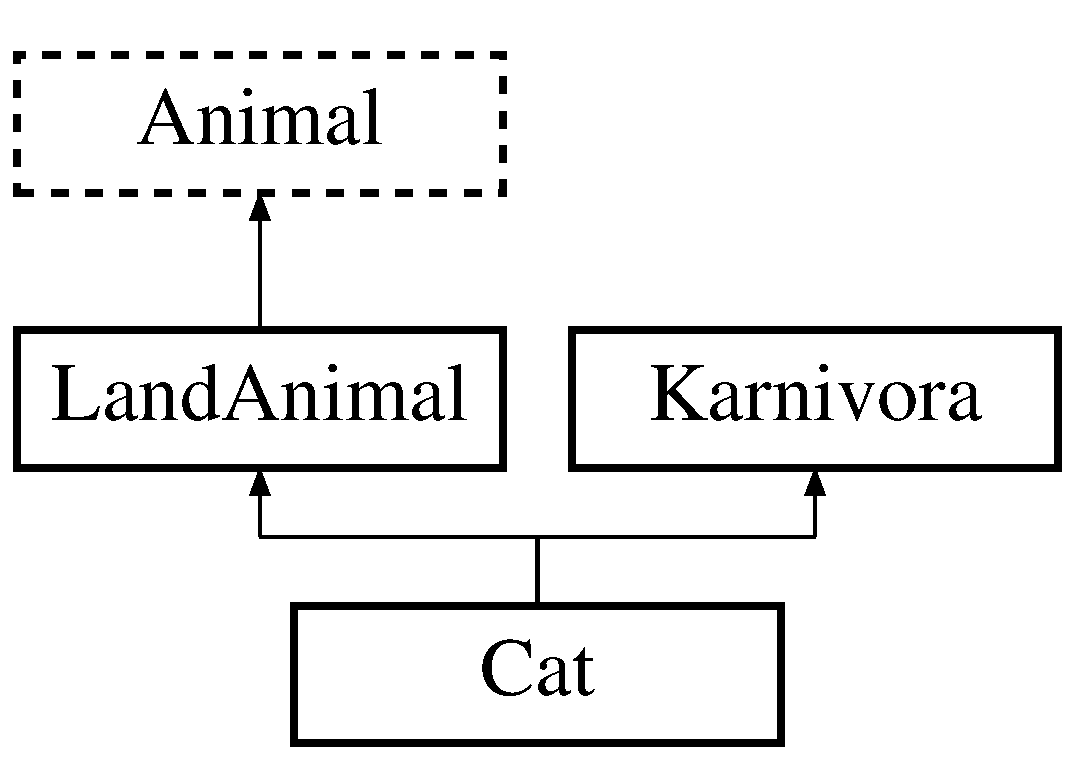
\includegraphics[height=3.000000cm]{classCat}
\end{center}
\end{figure}
\subsection*{Public Member Functions}
\begin{DoxyCompactItemize}
\item 
\hyperlink{classCat_a1dc60e85d1863d683c621f886dae1655}{Cat} (int \-\_\-x, int \-\_\-y)
\begin{DoxyCompactList}\small\item\em Constructor. \end{DoxyCompactList}\item 
\hypertarget{classCat_accae87693b84127a716243cbf5e6ddee}{\hyperlink{classCat_accae87693b84127a716243cbf5e6ddee}{$\sim$\-Cat} ()}\label{classCat_accae87693b84127a716243cbf5e6ddee}

\begin{DoxyCompactList}\small\item\em Destructor. \end{DoxyCompactList}\item 
\hypertarget{classCat_a72639929e5e40bbf1f6af6cc72e43717}{void \hyperlink{classCat_a72639929e5e40bbf1f6af6cc72e43717}{add\-Bobot} ()}\label{classCat_a72639929e5e40bbf1f6af6cc72e43717}

\begin{DoxyCompactList}\small\item\em Menambahkan bobot satu satuan. \end{DoxyCompactList}\item 
int \hyperlink{classCat_a6469896b2a5cf71f1059cb6160c5ab1c}{get\-Bobot} ()
\begin{DoxyCompactList}\small\item\em Mendapatkan nilai bobot dari \hyperlink{classCat}{Cat}. \end{DoxyCompactList}\item 
char \hyperlink{classCat_aa5dcbb810672c41de7419448f152b111}{get\-Simbol} ()
\begin{DoxyCompactList}\small\item\em Mendapatkan simbol dari \hyperlink{classCat}{Cat}. \end{DoxyCompactList}\item 
string \hyperlink{classCat_a385ab3b94c22ab9193d3399d56c4f8df}{get\-Musuh} (int i)
\begin{DoxyCompactList}\small\item\em Mendapatkan musuh ke i dari \hyperlink{classCat}{Cat} Musuh merupakan \hyperlink{classAnimal}{Animal} lain yang tidak bisa tinggal dalam satu kandang dengan \hyperlink{classCat}{Cat}. \end{DoxyCompactList}\item 
string \hyperlink{classCat_aea67aec6bb71b1fddbb04457a4ac8686}{interact} ()
\begin{DoxyCompactList}\small\item\em Mendapatkan reaksi \hyperlink{classCat}{Cat} saat berinteraksi dengan pengunjung. \end{DoxyCompactList}\item 
string \hyperlink{classCat_afdfbeb800c542a10a79151d2d7519ac3}{get\-Tipe\-Animal} ()
\begin{DoxyCompactList}\small\item\em Mendapatkan tipe \hyperlink{classAnimal}{Animal} (nama spesies) \end{DoxyCompactList}\end{DoxyCompactItemize}
\subsection*{Protected Attributes}
\begin{DoxyCompactItemize}
\item 
\hypertarget{classCat_ab1c3d1a4bf864f0de661053f28dbc777}{const string {\bfseries tipe\-Animal} = \char`\"{}cat\char`\"{}}\label{classCat_ab1c3d1a4bf864f0de661053f28dbc777}

\item 
\hypertarget{classCat_a941269c1c7b2aab846372691ede85bd2}{const char {\bfseries simbol} = 'c'}\label{classCat_a941269c1c7b2aab846372691ede85bd2}

\item 
\hypertarget{classCat_a874bc68a3d8ecd45dd98d8399fe9a14f}{int {\bfseries bobot}}\label{classCat_a874bc68a3d8ecd45dd98d8399fe9a14f}

\item 
\hypertarget{classCat_a8cbf92af5c962fe13c47eb110b3f95e9}{string $\ast$ {\bfseries musuh}}\label{classCat_a8cbf92af5c962fe13c47eb110b3f95e9}

\end{DoxyCompactItemize}


\subsection{Detailed Description}
Merupakan \hyperlink{classAnimal}{Animal} yang tinggal di darat dan merupakan \hyperlink{classKarnivora}{Karnivora} 

\subsection{Constructor \& Destructor Documentation}
\hypertarget{classCat_a1dc60e85d1863d683c621f886dae1655}{\index{Cat@{Cat}!Cat@{Cat}}
\index{Cat@{Cat}!Cat@{Cat}}
\subsubsection[{Cat}]{\setlength{\rightskip}{0pt plus 5cm}Cat\-::\-Cat (
\begin{DoxyParamCaption}
\item[{int}]{\-\_\-x, }
\item[{int}]{\-\_\-y}
\end{DoxyParamCaption}
)}}\label{classCat_a1dc60e85d1863d683c621f886dae1655}


Constructor. 


\begin{DoxyParams}{Parameters}
{\em \-\_\-x} & posisi x awal \hyperlink{classCat}{Cat} \\
\hline
{\em \-\_\-y} & posisi y awal \hyperlink{classCat}{Cat} \\
\hline
\end{DoxyParams}


\subsection{Member Function Documentation}
\hypertarget{classCat_a6469896b2a5cf71f1059cb6160c5ab1c}{\index{Cat@{Cat}!get\-Bobot@{get\-Bobot}}
\index{get\-Bobot@{get\-Bobot}!Cat@{Cat}}
\subsubsection[{get\-Bobot}]{\setlength{\rightskip}{0pt plus 5cm}int Cat\-::get\-Bobot (
\begin{DoxyParamCaption}
{}
\end{DoxyParamCaption}
)\hspace{0.3cm}{\ttfamily [virtual]}}}\label{classCat_a6469896b2a5cf71f1059cb6160c5ab1c}


Mendapatkan nilai bobot dari \hyperlink{classCat}{Cat}. 

\begin{DoxyReturn}{Returns}
bobot 
\end{DoxyReturn}


Implements \hyperlink{classAnimal}{Animal}.

\hypertarget{classCat_a385ab3b94c22ab9193d3399d56c4f8df}{\index{Cat@{Cat}!get\-Musuh@{get\-Musuh}}
\index{get\-Musuh@{get\-Musuh}!Cat@{Cat}}
\subsubsection[{get\-Musuh}]{\setlength{\rightskip}{0pt plus 5cm}string Cat\-::get\-Musuh (
\begin{DoxyParamCaption}
\item[{int}]{i}
\end{DoxyParamCaption}
)\hspace{0.3cm}{\ttfamily [virtual]}}}\label{classCat_a385ab3b94c22ab9193d3399d56c4f8df}


Mendapatkan musuh ke i dari \hyperlink{classCat}{Cat} Musuh merupakan \hyperlink{classAnimal}{Animal} lain yang tidak bisa tinggal dalam satu kandang dengan \hyperlink{classCat}{Cat}. 

\begin{DoxyReturn}{Returns}
musuh\mbox{[}i\mbox{]} 
\end{DoxyReturn}


Implements \hyperlink{classAnimal}{Animal}.

\hypertarget{classCat_aa5dcbb810672c41de7419448f152b111}{\index{Cat@{Cat}!get\-Simbol@{get\-Simbol}}
\index{get\-Simbol@{get\-Simbol}!Cat@{Cat}}
\subsubsection[{get\-Simbol}]{\setlength{\rightskip}{0pt plus 5cm}char Cat\-::get\-Simbol (
\begin{DoxyParamCaption}
{}
\end{DoxyParamCaption}
)\hspace{0.3cm}{\ttfamily [virtual]}}}\label{classCat_aa5dcbb810672c41de7419448f152b111}


Mendapatkan simbol dari \hyperlink{classCat}{Cat}. 

\begin{DoxyReturn}{Returns}
simbol 
\end{DoxyReturn}


Implements \hyperlink{classAnimal}{Animal}.

\hypertarget{classCat_afdfbeb800c542a10a79151d2d7519ac3}{\index{Cat@{Cat}!get\-Tipe\-Animal@{get\-Tipe\-Animal}}
\index{get\-Tipe\-Animal@{get\-Tipe\-Animal}!Cat@{Cat}}
\subsubsection[{get\-Tipe\-Animal}]{\setlength{\rightskip}{0pt plus 5cm}string Cat\-::get\-Tipe\-Animal (
\begin{DoxyParamCaption}
{}
\end{DoxyParamCaption}
)\hspace{0.3cm}{\ttfamily [virtual]}}}\label{classCat_afdfbeb800c542a10a79151d2d7519ac3}


Mendapatkan tipe \hyperlink{classAnimal}{Animal} (nama spesies) 

\begin{DoxyReturn}{Returns}
tipe\-Animal 
\end{DoxyReturn}


Implements \hyperlink{classLandAnimal}{Land\-Animal}.

\hypertarget{classCat_aea67aec6bb71b1fddbb04457a4ac8686}{\index{Cat@{Cat}!interact@{interact}}
\index{interact@{interact}!Cat@{Cat}}
\subsubsection[{interact}]{\setlength{\rightskip}{0pt plus 5cm}string Cat\-::interact (
\begin{DoxyParamCaption}
{}
\end{DoxyParamCaption}
)\hspace{0.3cm}{\ttfamily [virtual]}}}\label{classCat_aea67aec6bb71b1fddbb04457a4ac8686}


Mendapatkan reaksi \hyperlink{classCat}{Cat} saat berinteraksi dengan pengunjung. 

\begin{DoxyReturn}{Returns}
\char`\"{}meowmeow\char`\"{} 
\end{DoxyReturn}


Implements \hyperlink{classLandAnimal}{Land\-Animal}.



The documentation for this class was generated from the following files\-:\begin{DoxyCompactItemize}
\item 
Cat.\-h\item 
Cat.\-cpp\end{DoxyCompactItemize}

\hypertarget{classCell}{\section{Cell Class Reference}
\label{classCell}\index{Cell@{Cell}}
}


{\ttfamily \#include $<$Cell.\-h$>$}

Inheritance diagram for Cell\-:\begin{figure}[H]
\begin{center}
\leavevmode
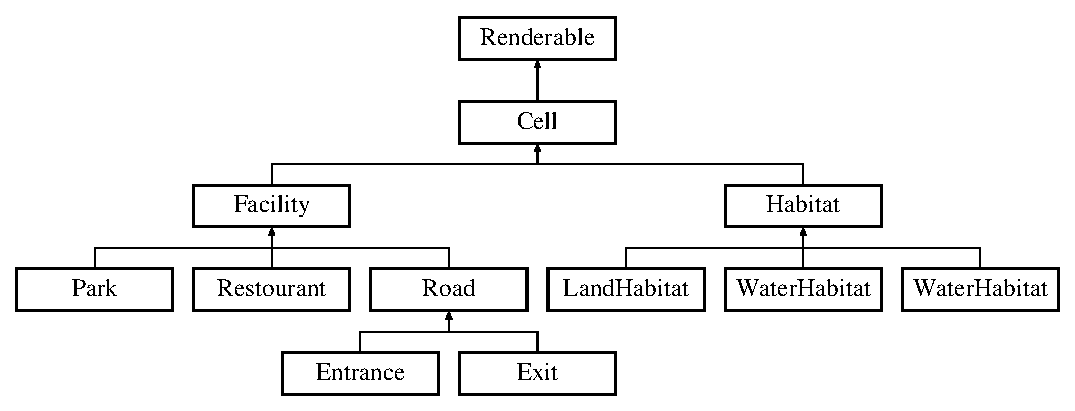
\includegraphics[height=5.000000cm]{classCell}
\end{center}
\end{figure}
\subsection*{Public Member Functions}
\begin{DoxyCompactItemize}
\item 
\hyperlink{classCell_a2cdce2f976b12fb50d1b9ca10c7e3b7d}{Cell} (int x, int y, char s)
\begin{DoxyCompactList}\small\item\em Constructor. \end{DoxyCompactList}\item 
virtual string \hyperlink{classCell_acf75f66796e8746df81dec0f7700ebbc}{get\-Tipe} ()=0
\begin{DoxyCompactList}\small\item\em Mendapatkan tipe \hyperlink{classCell}{Cell}. \end{DoxyCompactList}\item 
int \hyperlink{classCell_aab1e15a21ebcf0264bb79ec70224289c}{get\-X} ()
\begin{DoxyCompactList}\small\item\em Mendapatkan x. \end{DoxyCompactList}\item 
int \hyperlink{classCell_aa3afa71b2bb12f59bec1a06ffb3d4b5a}{get\-Y} ()
\begin{DoxyCompactList}\small\item\em Mendapatkan y. \end{DoxyCompactList}\item 
void \hyperlink{classCell_a5f610c860182564a7772d092204bc72d}{set\-X} (int a)
\begin{DoxyCompactList}\small\item\em Mengganti nilai x \hyperlink{classCell}{Cell} dengan nilai a. \end{DoxyCompactList}\item 
void \hyperlink{classCell_afe18f178541bac6004586866f2fb684c}{set\-Y} (int b)
\begin{DoxyCompactList}\small\item\em Mengganti nilai y \hyperlink{classCell}{Cell} dengan nilai b. \end{DoxyCompactList}\item 
char \hyperlink{classCell_a1fc51c6f42b94d1e55f41f068846f523}{render} ()
\begin{DoxyCompactList}\small\item\em Mengembalika karakter symbol dari \hyperlink{classCell}{Cell}. \end{DoxyCompactList}\end{DoxyCompactItemize}


\subsection{Detailed Description}
Kelas \hyperlink{classCell}{Cell} menyatakan petak pada Virtual Zoo. Merupakan turunan dari kelas \hyperlink{classRenderable}{Renderable}. 

\subsection{Constructor \& Destructor Documentation}
\hypertarget{classCell_a2cdce2f976b12fb50d1b9ca10c7e3b7d}{\index{Cell@{Cell}!Cell@{Cell}}
\index{Cell@{Cell}!Cell@{Cell}}
\subsubsection[{Cell}]{\setlength{\rightskip}{0pt plus 5cm}Cell\-::\-Cell (
\begin{DoxyParamCaption}
\item[{int}]{x, }
\item[{int}]{y, }
\item[{char}]{s}
\end{DoxyParamCaption}
)}}\label{classCell_a2cdce2f976b12fb50d1b9ca10c7e3b7d}


Constructor. 


\begin{DoxyParams}{Parameters}
{\em x} & Indeks baris \\
\hline
{\em y} & Indeks kolom \\
\hline
{\em s} & Simbol \\
\hline
\end{DoxyParams}


\subsection{Member Function Documentation}
\hypertarget{classCell_acf75f66796e8746df81dec0f7700ebbc}{\index{Cell@{Cell}!get\-Tipe@{get\-Tipe}}
\index{get\-Tipe@{get\-Tipe}!Cell@{Cell}}
\subsubsection[{get\-Tipe}]{\setlength{\rightskip}{0pt plus 5cm}virtual string Cell\-::get\-Tipe (
\begin{DoxyParamCaption}
{}
\end{DoxyParamCaption}
)\hspace{0.3cm}{\ttfamily [pure virtual]}}}\label{classCell_acf75f66796e8746df81dec0f7700ebbc}


Mendapatkan tipe \hyperlink{classCell}{Cell}. 

\begin{DoxyReturn}{Returns}
tipe 
\end{DoxyReturn}


Implemented in \hyperlink{classWaterHabitat_a02b4e524ab689f2e2b54b74acb58f7b2}{Water\-Habitat}, \hyperlink{classEntrance_afff61031d269e47536b3bf4821ab0dda}{Entrance}, \hyperlink{classExit_aa769d720f40b684da6ca21fc2515f910}{Exit}, \hyperlink{classFacility_a0350c1492460c160c95b1be72ea09860}{Facility}, \hyperlink{classHabitat_a4c8164f06a0a32ca6c7f465380b31ac0}{Habitat}, \hyperlink{classLandHabitat_a51ad769f1682ec5b45bcd8839e854575}{Land\-Habitat}, \hyperlink{classPark_a2b8533d7c9e2024ccc58c57f89f192f2}{Park}, \hyperlink{classRestourant_a5f4f9f7229416a7c339bc08c7a50a991}{Restourant}, \hyperlink{classRoad_a750f8b4ab694ed29e8bd6db4d9758429}{Road}, and \hyperlink{classWaterHabitat_a02b4e524ab689f2e2b54b74acb58f7b2}{Water\-Habitat}.

\hypertarget{classCell_aab1e15a21ebcf0264bb79ec70224289c}{\index{Cell@{Cell}!get\-X@{get\-X}}
\index{get\-X@{get\-X}!Cell@{Cell}}
\subsubsection[{get\-X}]{\setlength{\rightskip}{0pt plus 5cm}int Cell\-::get\-X (
\begin{DoxyParamCaption}
{}
\end{DoxyParamCaption}
)}}\label{classCell_aab1e15a21ebcf0264bb79ec70224289c}


Mendapatkan x. 

\begin{DoxyReturn}{Returns}
x posisi x dari \hyperlink{classCell}{Cell} 
\end{DoxyReturn}
\hypertarget{classCell_aa3afa71b2bb12f59bec1a06ffb3d4b5a}{\index{Cell@{Cell}!get\-Y@{get\-Y}}
\index{get\-Y@{get\-Y}!Cell@{Cell}}
\subsubsection[{get\-Y}]{\setlength{\rightskip}{0pt plus 5cm}int Cell\-::get\-Y (
\begin{DoxyParamCaption}
{}
\end{DoxyParamCaption}
)}}\label{classCell_aa3afa71b2bb12f59bec1a06ffb3d4b5a}


Mendapatkan y. 

\begin{DoxyReturn}{Returns}
y posisi y dari \hyperlink{classCell}{Cell} 
\end{DoxyReturn}
\hypertarget{classCell_a1fc51c6f42b94d1e55f41f068846f523}{\index{Cell@{Cell}!render@{render}}
\index{render@{render}!Cell@{Cell}}
\subsubsection[{render}]{\setlength{\rightskip}{0pt plus 5cm}char Cell\-::render (
\begin{DoxyParamCaption}
{}
\end{DoxyParamCaption}
)\hspace{0.3cm}{\ttfamily [virtual]}}}\label{classCell_a1fc51c6f42b94d1e55f41f068846f523}


Mengembalika karakter symbol dari \hyperlink{classCell}{Cell}. 

\begin{DoxyReturn}{Returns}
symbol 
\end{DoxyReturn}


Implements \hyperlink{classRenderable_aafa9280e6dcfa557b3cd675221fd97b4}{Renderable}.

\hypertarget{classCell_a5f610c860182564a7772d092204bc72d}{\index{Cell@{Cell}!set\-X@{set\-X}}
\index{set\-X@{set\-X}!Cell@{Cell}}
\subsubsection[{set\-X}]{\setlength{\rightskip}{0pt plus 5cm}void Cell\-::set\-X (
\begin{DoxyParamCaption}
\item[{int}]{a}
\end{DoxyParamCaption}
)}}\label{classCell_a5f610c860182564a7772d092204bc72d}


Mengganti nilai x \hyperlink{classCell}{Cell} dengan nilai a. 


\begin{DoxyParams}{Parameters}
{\em a} & Nilai yang akan menggantikan x \\
\hline
\end{DoxyParams}
\hypertarget{classCell_afe18f178541bac6004586866f2fb684c}{\index{Cell@{Cell}!set\-Y@{set\-Y}}
\index{set\-Y@{set\-Y}!Cell@{Cell}}
\subsubsection[{set\-Y}]{\setlength{\rightskip}{0pt plus 5cm}void Cell\-::set\-Y (
\begin{DoxyParamCaption}
\item[{int}]{b}
\end{DoxyParamCaption}
)}}\label{classCell_afe18f178541bac6004586866f2fb684c}


Mengganti nilai y \hyperlink{classCell}{Cell} dengan nilai b. 


\begin{DoxyParams}{Parameters}
{\em b} & Nilai yang akan menggantikan y \\
\hline
\end{DoxyParams}


The documentation for this class was generated from the following files\-:\begin{DoxyCompactItemize}
\item 
Cell.\-h\item 
Cell.\-cpp\end{DoxyCompactItemize}

\hypertarget{classChicken}{\section{Chicken Class Reference}
\label{classChicken}\index{Chicken@{Chicken}}
}


{\ttfamily \#include $<$Chicken.\-h$>$}

Inheritance diagram for Chicken\-:\begin{figure}[H]
\begin{center}
\leavevmode
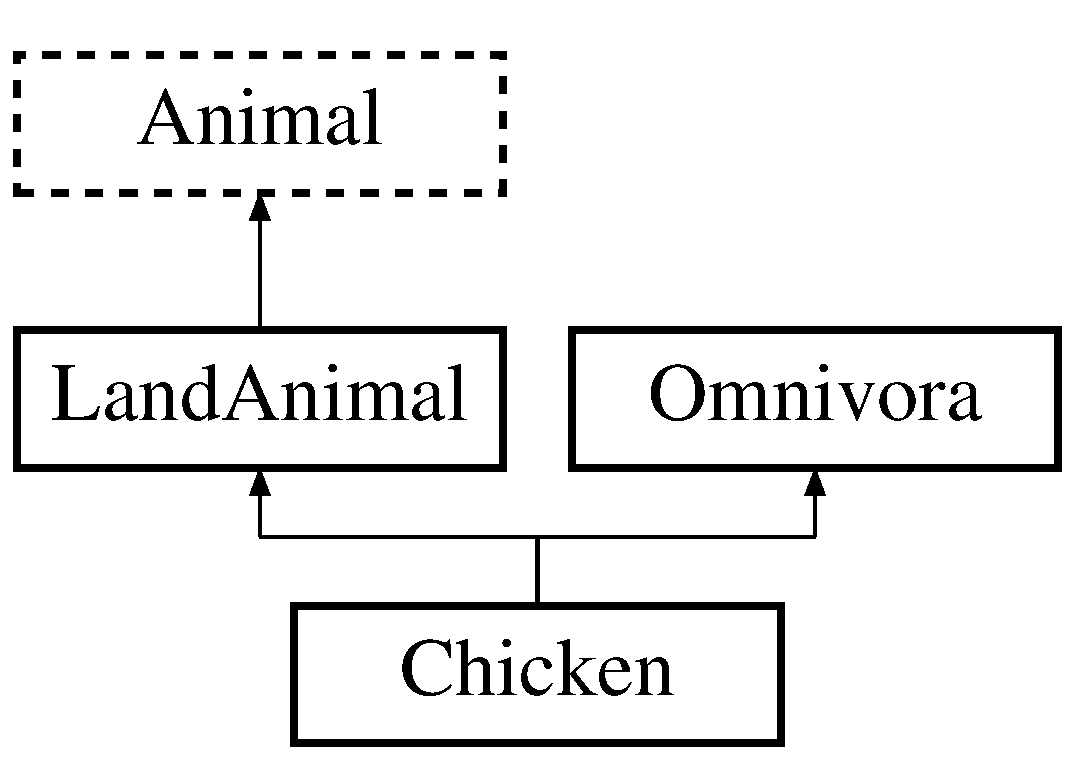
\includegraphics[height=3.000000cm]{classChicken}
\end{center}
\end{figure}
\subsection*{Public Member Functions}
\begin{DoxyCompactItemize}
\item 
\hyperlink{classChicken_a4ca0ca08ac03410d9551564b7bf77c8d}{Chicken} (int \-\_\-x, int \-\_\-y)
\begin{DoxyCompactList}\small\item\em Constructor. \end{DoxyCompactList}\item 
\hypertarget{classChicken_a467a41f21fa2b076f6f2d398c8e1ada8}{\hyperlink{classChicken_a467a41f21fa2b076f6f2d398c8e1ada8}{$\sim$\-Chicken} ()}\label{classChicken_a467a41f21fa2b076f6f2d398c8e1ada8}

\begin{DoxyCompactList}\small\item\em Destructor. \end{DoxyCompactList}\item 
\hypertarget{classChicken_acbcd8ace889db2287c8494dbd7c8a38b}{void \hyperlink{classChicken_acbcd8ace889db2287c8494dbd7c8a38b}{add\-Bobot} ()}\label{classChicken_acbcd8ace889db2287c8494dbd7c8a38b}

\begin{DoxyCompactList}\small\item\em Menambahkan bobot satu satuan. \end{DoxyCompactList}\item 
int \hyperlink{classChicken_a3412b91656f7fbc582e61347d041fc26}{get\-Bobot} ()
\begin{DoxyCompactList}\small\item\em Mendapatkan nilai bobot dari \hyperlink{classChicken}{Chicken}. \end{DoxyCompactList}\item 
char \hyperlink{classChicken_a76ccfbab33c1e7e8586594d5a187f24f}{get\-Simbol} ()
\begin{DoxyCompactList}\small\item\em Mendapatkan simbol dari \hyperlink{classChicken}{Chicken}. \end{DoxyCompactList}\item 
string \hyperlink{classChicken_a3104bf975190b71c598c8a9190cc8e82}{get\-Musuh} (int i)
\begin{DoxyCompactList}\small\item\em Mendapatkan musuh ke i dari \hyperlink{classChicken}{Chicken} Musuh merupakan \hyperlink{classAnimal}{Animal} lain yang tidak bisa tinggal dalam satu kandang dengan \hyperlink{classChicken}{Chicken}. \end{DoxyCompactList}\item 
string \hyperlink{classChicken_a4b257cd1beddc7998245e1a276be9538}{interact} ()
\begin{DoxyCompactList}\small\item\em Mendapatkan reaksi \hyperlink{classChicken}{Chicken} saat berinteraksi dengan pengunjung. \end{DoxyCompactList}\item 
string \hyperlink{classChicken_aed9dc3fbf2e9a352d27109ba331db37d}{get\-Tipe\-Animal} ()
\begin{DoxyCompactList}\small\item\em Mendapatkan tipe \hyperlink{classAnimal}{Animal} (nama spesies) \end{DoxyCompactList}\end{DoxyCompactItemize}
\subsection*{Protected Attributes}
\begin{DoxyCompactItemize}
\item 
\hypertarget{classChicken_a2ab48bb09746cb546a0dd2d295f2d2da}{const string {\bfseries tipe\-Animal} = \char`\"{}chicken\char`\"{}}\label{classChicken_a2ab48bb09746cb546a0dd2d295f2d2da}

\item 
\hypertarget{classChicken_a543298297ce0ffa9441a11f8298ac5fa}{const char {\bfseries simbol} = 'n'}\label{classChicken_a543298297ce0ffa9441a11f8298ac5fa}

\item 
\hypertarget{classChicken_a9ec3ad294e2af757b8a467294c420ebb}{int {\bfseries bobot}}\label{classChicken_a9ec3ad294e2af757b8a467294c420ebb}

\item 
\hypertarget{classChicken_ad06a7254bedeb9b76d7f0598f552a4d3}{string $\ast$ {\bfseries musuh}}\label{classChicken_ad06a7254bedeb9b76d7f0598f552a4d3}

\end{DoxyCompactItemize}


\subsection{Detailed Description}
Merupakan \hyperlink{classAnimal}{Animal} yang tinggal di darat dan merupakan \hyperlink{classOmnivora}{Omnivora} 

\subsection{Constructor \& Destructor Documentation}
\hypertarget{classChicken_a4ca0ca08ac03410d9551564b7bf77c8d}{\index{Chicken@{Chicken}!Chicken@{Chicken}}
\index{Chicken@{Chicken}!Chicken@{Chicken}}
\subsubsection[{Chicken}]{\setlength{\rightskip}{0pt plus 5cm}Chicken\-::\-Chicken (
\begin{DoxyParamCaption}
\item[{int}]{\-\_\-x, }
\item[{int}]{\-\_\-y}
\end{DoxyParamCaption}
)}}\label{classChicken_a4ca0ca08ac03410d9551564b7bf77c8d}


Constructor. 


\begin{DoxyParams}{Parameters}
{\em \-\_\-x} & posisi x awal \hyperlink{classChicken}{Chicken} \\
\hline
{\em \-\_\-y} & posisi y awal \hyperlink{classChicken}{Chicken} \\
\hline
\end{DoxyParams}


\subsection{Member Function Documentation}
\hypertarget{classChicken_a3412b91656f7fbc582e61347d041fc26}{\index{Chicken@{Chicken}!get\-Bobot@{get\-Bobot}}
\index{get\-Bobot@{get\-Bobot}!Chicken@{Chicken}}
\subsubsection[{get\-Bobot}]{\setlength{\rightskip}{0pt plus 5cm}int Chicken\-::get\-Bobot (
\begin{DoxyParamCaption}
{}
\end{DoxyParamCaption}
)\hspace{0.3cm}{\ttfamily [virtual]}}}\label{classChicken_a3412b91656f7fbc582e61347d041fc26}


Mendapatkan nilai bobot dari \hyperlink{classChicken}{Chicken}. 

\begin{DoxyReturn}{Returns}
bobot 
\end{DoxyReturn}


Implements \hyperlink{classAnimal}{Animal}.

\hypertarget{classChicken_a3104bf975190b71c598c8a9190cc8e82}{\index{Chicken@{Chicken}!get\-Musuh@{get\-Musuh}}
\index{get\-Musuh@{get\-Musuh}!Chicken@{Chicken}}
\subsubsection[{get\-Musuh}]{\setlength{\rightskip}{0pt plus 5cm}string Chicken\-::get\-Musuh (
\begin{DoxyParamCaption}
\item[{int}]{i}
\end{DoxyParamCaption}
)\hspace{0.3cm}{\ttfamily [virtual]}}}\label{classChicken_a3104bf975190b71c598c8a9190cc8e82}


Mendapatkan musuh ke i dari \hyperlink{classChicken}{Chicken} Musuh merupakan \hyperlink{classAnimal}{Animal} lain yang tidak bisa tinggal dalam satu kandang dengan \hyperlink{classChicken}{Chicken}. 

\begin{DoxyReturn}{Returns}
musuh\mbox{[}i\mbox{]} 
\end{DoxyReturn}


Implements \hyperlink{classAnimal}{Animal}.

\hypertarget{classChicken_a76ccfbab33c1e7e8586594d5a187f24f}{\index{Chicken@{Chicken}!get\-Simbol@{get\-Simbol}}
\index{get\-Simbol@{get\-Simbol}!Chicken@{Chicken}}
\subsubsection[{get\-Simbol}]{\setlength{\rightskip}{0pt plus 5cm}char Chicken\-::get\-Simbol (
\begin{DoxyParamCaption}
{}
\end{DoxyParamCaption}
)\hspace{0.3cm}{\ttfamily [virtual]}}}\label{classChicken_a76ccfbab33c1e7e8586594d5a187f24f}


Mendapatkan simbol dari \hyperlink{classChicken}{Chicken}. 

\begin{DoxyReturn}{Returns}
simbol 
\end{DoxyReturn}


Implements \hyperlink{classAnimal}{Animal}.

\hypertarget{classChicken_aed9dc3fbf2e9a352d27109ba331db37d}{\index{Chicken@{Chicken}!get\-Tipe\-Animal@{get\-Tipe\-Animal}}
\index{get\-Tipe\-Animal@{get\-Tipe\-Animal}!Chicken@{Chicken}}
\subsubsection[{get\-Tipe\-Animal}]{\setlength{\rightskip}{0pt plus 5cm}string Chicken\-::get\-Tipe\-Animal (
\begin{DoxyParamCaption}
{}
\end{DoxyParamCaption}
)\hspace{0.3cm}{\ttfamily [virtual]}}}\label{classChicken_aed9dc3fbf2e9a352d27109ba331db37d}


Mendapatkan tipe \hyperlink{classAnimal}{Animal} (nama spesies) 

\begin{DoxyReturn}{Returns}
tipe\-Animal 
\end{DoxyReturn}


Implements \hyperlink{classLandAnimal}{Land\-Animal}.

\hypertarget{classChicken_a4b257cd1beddc7998245e1a276be9538}{\index{Chicken@{Chicken}!interact@{interact}}
\index{interact@{interact}!Chicken@{Chicken}}
\subsubsection[{interact}]{\setlength{\rightskip}{0pt plus 5cm}string Chicken\-::interact (
\begin{DoxyParamCaption}
{}
\end{DoxyParamCaption}
)\hspace{0.3cm}{\ttfamily [virtual]}}}\label{classChicken_a4b257cd1beddc7998245e1a276be9538}


Mendapatkan reaksi \hyperlink{classChicken}{Chicken} saat berinteraksi dengan pengunjung. 

\begin{DoxyReturn}{Returns}
\char`\"{}chipchip\char`\"{} 
\end{DoxyReturn}


Implements \hyperlink{classLandAnimal}{Land\-Animal}.



The documentation for this class was generated from the following files\-:\begin{DoxyCompactItemize}
\item 
Chicken.\-h\item 
Chicken.\-cpp\end{DoxyCompactItemize}

\hypertarget{classCow}{\section{Cow Class Reference}
\label{classCow}\index{Cow@{Cow}}
}


{\ttfamily \#include $<$Cow.\-h$>$}

Inheritance diagram for Cow\-:\begin{figure}[H]
\begin{center}
\leavevmode
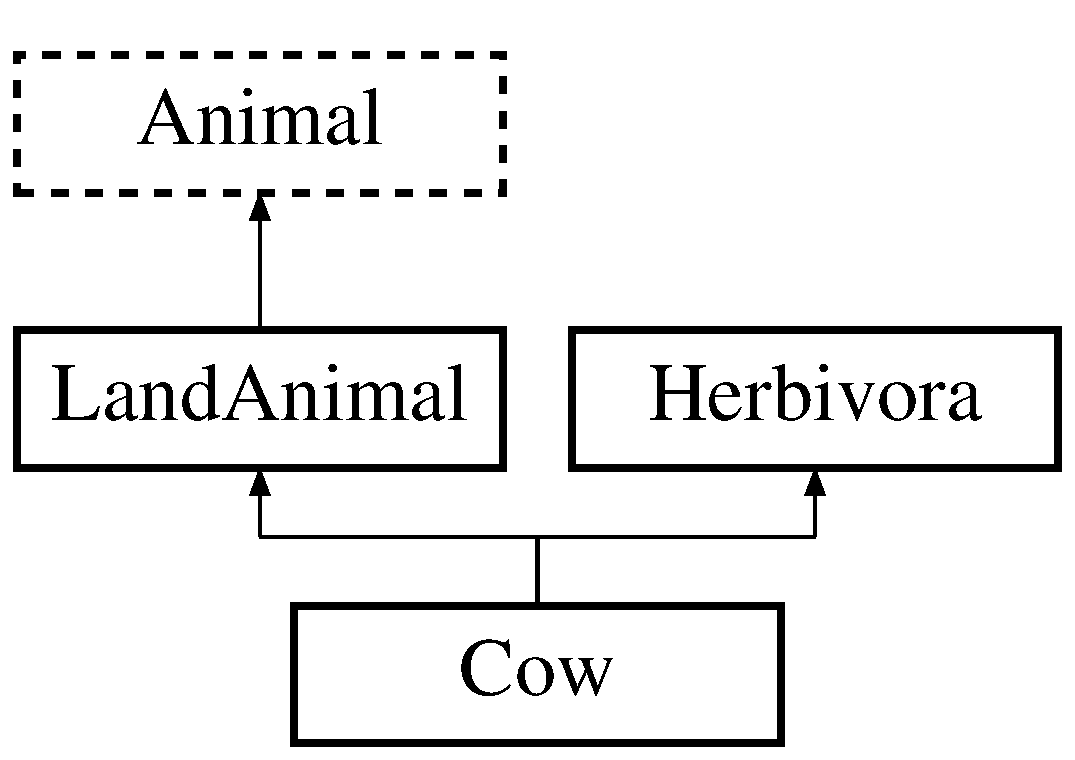
\includegraphics[height=3.000000cm]{classCow}
\end{center}
\end{figure}
\subsection*{Public Member Functions}
\begin{DoxyCompactItemize}
\item 
\hyperlink{classCow_a8d004e3d53acceb83ac4321f972fc78b}{Cow} (int \-\_\-x, int \-\_\-y)
\begin{DoxyCompactList}\small\item\em Constructor. \end{DoxyCompactList}\item 
\hypertarget{classCow_ab6e5749431c51b7d1cda263fcd48393a}{\hyperlink{classCow_ab6e5749431c51b7d1cda263fcd48393a}{$\sim$\-Cow} ()}\label{classCow_ab6e5749431c51b7d1cda263fcd48393a}

\begin{DoxyCompactList}\small\item\em Destructor. \end{DoxyCompactList}\item 
\hypertarget{classCow_a33b115281c154d17f259c18fff1f4d3a}{void \hyperlink{classCow_a33b115281c154d17f259c18fff1f4d3a}{add\-Bobot} ()}\label{classCow_a33b115281c154d17f259c18fff1f4d3a}

\begin{DoxyCompactList}\small\item\em Menambahkan bobot satu satuan. \end{DoxyCompactList}\item 
int \hyperlink{classCow_a64435a687437ce3db8cf38be1984737c}{get\-Bobot} ()
\begin{DoxyCompactList}\small\item\em Mendapatkan nilai bobot dari \hyperlink{classCow}{Cow}. \end{DoxyCompactList}\item 
char \hyperlink{classCow_a2f52ce339a0ee1d19e32ff2010a8ea68}{get\-Simbol} ()
\begin{DoxyCompactList}\small\item\em Mendapatkan simbol dari \hyperlink{classCow}{Cow}. \end{DoxyCompactList}\item 
string \hyperlink{classCow_a006b5864bd414238ae9337dfa8ca193a}{get\-Musuh} (int i)
\begin{DoxyCompactList}\small\item\em Mendapatkan musuh ke i dari \hyperlink{classCow}{Cow} Musuh merupakan \hyperlink{classAnimal}{Animal} lain yang tidak bisa tinggal dalam satu kandang dengan \hyperlink{classCow}{Cow}. \end{DoxyCompactList}\item 
string \hyperlink{classCow_a1299050bf0fa6e933d22d7027428d885}{interact} ()
\begin{DoxyCompactList}\small\item\em Mendapatkan reaksi \hyperlink{classCow}{Cow} saat berinteraksi dengan pengunjung. \end{DoxyCompactList}\item 
string \hyperlink{classCow_aff355d86a92e62f6c3be421173064f3b}{get\-Tipe\-Animal} ()
\begin{DoxyCompactList}\small\item\em Mendapatkan tipe \hyperlink{classAnimal}{Animal} (nama spesies) \end{DoxyCompactList}\end{DoxyCompactItemize}
\subsection*{Protected Attributes}
\begin{DoxyCompactItemize}
\item 
\hypertarget{classCow_a3fe80551fc501157fe95d242fed693e7}{const string {\bfseries tipe\-Animal} = \char`\"{}cow\char`\"{}}\label{classCow_a3fe80551fc501157fe95d242fed693e7}

\item 
\hypertarget{classCow_a3e20a16a31cccbf3a4ed72df5d4245c0}{const char {\bfseries simbol} = 'w'}\label{classCow_a3e20a16a31cccbf3a4ed72df5d4245c0}

\item 
\hypertarget{classCow_a980a21c5e2127566fa263968aa82a881}{int {\bfseries bobot}}\label{classCow_a980a21c5e2127566fa263968aa82a881}

\item 
\hypertarget{classCow_a25e958ccec81f7b71fd68919ec0ff967}{string $\ast$ {\bfseries musuh}}\label{classCow_a25e958ccec81f7b71fd68919ec0ff967}

\end{DoxyCompactItemize}


\subsection{Detailed Description}
Merupakan \hyperlink{classAnimal}{Animal} yang tinggal di darat dan merupakan \hyperlink{classHerbivora}{Herbivora} 

\subsection{Constructor \& Destructor Documentation}
\hypertarget{classCow_a8d004e3d53acceb83ac4321f972fc78b}{\index{Cow@{Cow}!Cow@{Cow}}
\index{Cow@{Cow}!Cow@{Cow}}
\subsubsection[{Cow}]{\setlength{\rightskip}{0pt plus 5cm}Cow\-::\-Cow (
\begin{DoxyParamCaption}
\item[{int}]{\-\_\-x, }
\item[{int}]{\-\_\-y}
\end{DoxyParamCaption}
)}}\label{classCow_a8d004e3d53acceb83ac4321f972fc78b}


Constructor. 


\begin{DoxyParams}{Parameters}
{\em \-\_\-x} & posisi x awal \hyperlink{classCow}{Cow} \\
\hline
{\em \-\_\-y} & posisi y awal \hyperlink{classCow}{Cow} \\
\hline
\end{DoxyParams}


\subsection{Member Function Documentation}
\hypertarget{classCow_a64435a687437ce3db8cf38be1984737c}{\index{Cow@{Cow}!get\-Bobot@{get\-Bobot}}
\index{get\-Bobot@{get\-Bobot}!Cow@{Cow}}
\subsubsection[{get\-Bobot}]{\setlength{\rightskip}{0pt plus 5cm}int Cow\-::get\-Bobot (
\begin{DoxyParamCaption}
{}
\end{DoxyParamCaption}
)\hspace{0.3cm}{\ttfamily [virtual]}}}\label{classCow_a64435a687437ce3db8cf38be1984737c}


Mendapatkan nilai bobot dari \hyperlink{classCow}{Cow}. 

\begin{DoxyReturn}{Returns}
bobot 
\end{DoxyReturn}


Implements \hyperlink{classAnimal}{Animal}.

\hypertarget{classCow_a006b5864bd414238ae9337dfa8ca193a}{\index{Cow@{Cow}!get\-Musuh@{get\-Musuh}}
\index{get\-Musuh@{get\-Musuh}!Cow@{Cow}}
\subsubsection[{get\-Musuh}]{\setlength{\rightskip}{0pt plus 5cm}string Cow\-::get\-Musuh (
\begin{DoxyParamCaption}
\item[{int}]{i}
\end{DoxyParamCaption}
)\hspace{0.3cm}{\ttfamily [virtual]}}}\label{classCow_a006b5864bd414238ae9337dfa8ca193a}


Mendapatkan musuh ke i dari \hyperlink{classCow}{Cow} Musuh merupakan \hyperlink{classAnimal}{Animal} lain yang tidak bisa tinggal dalam satu kandang dengan \hyperlink{classCow}{Cow}. 

\begin{DoxyReturn}{Returns}
musuh\mbox{[}i\mbox{]} 
\end{DoxyReturn}


Implements \hyperlink{classAnimal}{Animal}.

\hypertarget{classCow_a2f52ce339a0ee1d19e32ff2010a8ea68}{\index{Cow@{Cow}!get\-Simbol@{get\-Simbol}}
\index{get\-Simbol@{get\-Simbol}!Cow@{Cow}}
\subsubsection[{get\-Simbol}]{\setlength{\rightskip}{0pt plus 5cm}char Cow\-::get\-Simbol (
\begin{DoxyParamCaption}
{}
\end{DoxyParamCaption}
)\hspace{0.3cm}{\ttfamily [virtual]}}}\label{classCow_a2f52ce339a0ee1d19e32ff2010a8ea68}


Mendapatkan simbol dari \hyperlink{classCow}{Cow}. 

\begin{DoxyReturn}{Returns}
simbol 
\end{DoxyReturn}


Implements \hyperlink{classAnimal}{Animal}.

\hypertarget{classCow_aff355d86a92e62f6c3be421173064f3b}{\index{Cow@{Cow}!get\-Tipe\-Animal@{get\-Tipe\-Animal}}
\index{get\-Tipe\-Animal@{get\-Tipe\-Animal}!Cow@{Cow}}
\subsubsection[{get\-Tipe\-Animal}]{\setlength{\rightskip}{0pt plus 5cm}string Cow\-::get\-Tipe\-Animal (
\begin{DoxyParamCaption}
{}
\end{DoxyParamCaption}
)\hspace{0.3cm}{\ttfamily [virtual]}}}\label{classCow_aff355d86a92e62f6c3be421173064f3b}


Mendapatkan tipe \hyperlink{classAnimal}{Animal} (nama spesies) 

\begin{DoxyReturn}{Returns}
tipe\-Animal 
\end{DoxyReturn}


Implements \hyperlink{classLandAnimal}{Land\-Animal}.

\hypertarget{classCow_a1299050bf0fa6e933d22d7027428d885}{\index{Cow@{Cow}!interact@{interact}}
\index{interact@{interact}!Cow@{Cow}}
\subsubsection[{interact}]{\setlength{\rightskip}{0pt plus 5cm}string Cow\-::interact (
\begin{DoxyParamCaption}
{}
\end{DoxyParamCaption}
)\hspace{0.3cm}{\ttfamily [virtual]}}}\label{classCow_a1299050bf0fa6e933d22d7027428d885}


Mendapatkan reaksi \hyperlink{classCow}{Cow} saat berinteraksi dengan pengunjung. 

\begin{DoxyReturn}{Returns}
\char`\"{}mooow\char`\"{} 
\end{DoxyReturn}


Implements \hyperlink{classLandAnimal}{Land\-Animal}.



The documentation for this class was generated from the following files\-:\begin{DoxyCompactItemize}
\item 
Cow.\-h\item 
Cow.\-cpp\end{DoxyCompactItemize}

\hypertarget{classCrocodile}{\section{Crocodile Class Reference}
\label{classCrocodile}\index{Crocodile@{Crocodile}}
}


{\ttfamily \#include $<$Crocodile.\-h$>$}

Inheritance diagram for Crocodile\-:\begin{figure}[H]
\begin{center}
\leavevmode
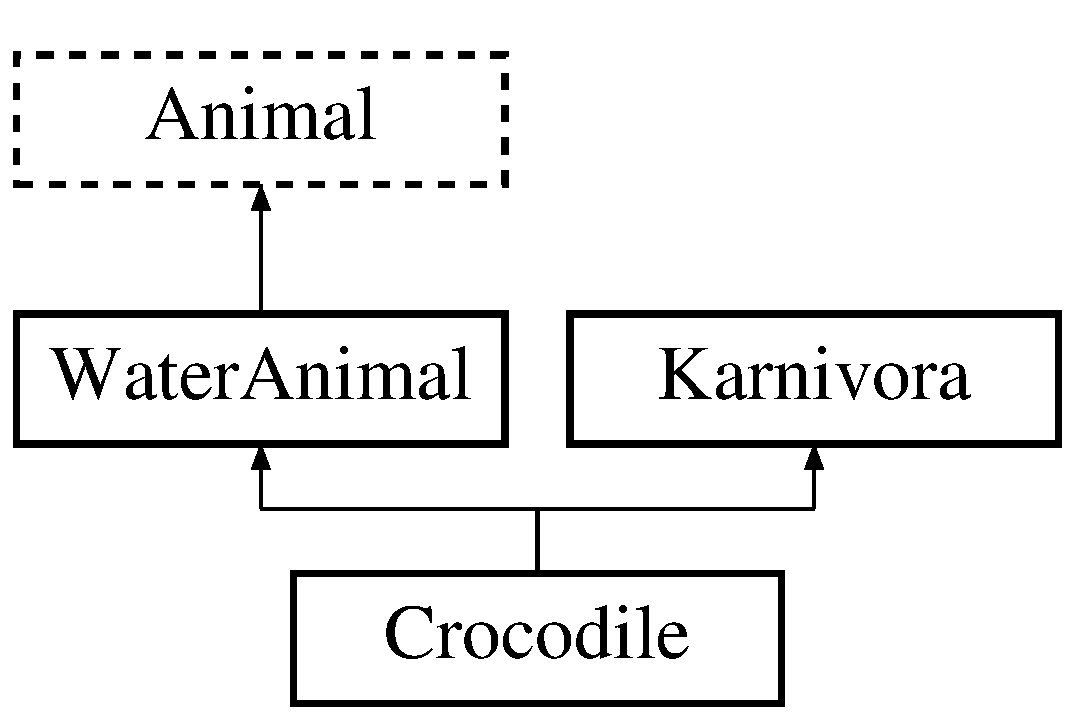
\includegraphics[height=3.000000cm]{classCrocodile}
\end{center}
\end{figure}
\subsection*{Public Member Functions}
\begin{DoxyCompactItemize}
\item 
\hyperlink{classCrocodile_abf158d817964be28b0a3fb555e195470}{Crocodile} (int \-\_\-x, int \-\_\-y)
\begin{DoxyCompactList}\small\item\em Constructor. \end{DoxyCompactList}\item 
\hypertarget{classCrocodile_aadc4a352f8baba14cdc08c20c46d92c0}{\hyperlink{classCrocodile_aadc4a352f8baba14cdc08c20c46d92c0}{$\sim$\-Crocodile} ()}\label{classCrocodile_aadc4a352f8baba14cdc08c20c46d92c0}

\begin{DoxyCompactList}\small\item\em Destructor. \end{DoxyCompactList}\item 
\hypertarget{classCrocodile_a993a3e8b0b5a3e6e48e9a4ac8e30a6ad}{void \hyperlink{classCrocodile_a993a3e8b0b5a3e6e48e9a4ac8e30a6ad}{add\-Bobot} ()}\label{classCrocodile_a993a3e8b0b5a3e6e48e9a4ac8e30a6ad}

\begin{DoxyCompactList}\small\item\em Menambahkan bobot satu satuan. \end{DoxyCompactList}\item 
int \hyperlink{classCrocodile_a9c767a7111f928236b068cae4445f631}{get\-Bobot} ()
\begin{DoxyCompactList}\small\item\em Mendapatkan nilai bobot dari \hyperlink{classCrocodile}{Crocodile}. \end{DoxyCompactList}\item 
char \hyperlink{classCrocodile_a924b698aef1f1d83761ebe0dea1f4510}{get\-Simbol} ()
\begin{DoxyCompactList}\small\item\em Mendapatkan simbol dari \hyperlink{classCrocodile}{Crocodile}. \end{DoxyCompactList}\item 
string \hyperlink{classCrocodile_abe0f3118e9e65974dc8693e0e118a149}{get\-Musuh} (int i)
\begin{DoxyCompactList}\small\item\em Mendapatkan musuh ke i dari \hyperlink{classCrocodile}{Crocodile} Musuh merupakan \hyperlink{classAnimal}{Animal} lain yang tidak bisa tinggal dalam satu kandang dengan \hyperlink{classCrocodile}{Crocodile}. \end{DoxyCompactList}\item 
string \hyperlink{classCrocodile_aeacbf1ca7d8d5549891604f1e2831dde}{interact} ()
\begin{DoxyCompactList}\small\item\em Mendapatkan reaksi \hyperlink{classCrocodile}{Crocodile} saat berinteraksi dengan pengunjung. \end{DoxyCompactList}\item 
string \hyperlink{classCrocodile_afe701f28f0d3471eeea91b1be20529b3}{get\-Tipe\-Animal} ()
\begin{DoxyCompactList}\small\item\em Mendapatkan tipe \hyperlink{classAnimal}{Animal} (nama spesies) \end{DoxyCompactList}\end{DoxyCompactItemize}
\subsection*{Protected Attributes}
\begin{DoxyCompactItemize}
\item 
\hypertarget{classCrocodile_a7ee03e8ea30bebbaa6d8c4eee4c81efe}{const string {\bfseries tipe\-Animal} = \char`\"{}crocodile\char`\"{}}\label{classCrocodile_a7ee03e8ea30bebbaa6d8c4eee4c81efe}

\item 
\hypertarget{classCrocodile_ad75207b26af7d5f9d95ab2a101b7722f}{const char {\bfseries simbol} = 'j'}\label{classCrocodile_ad75207b26af7d5f9d95ab2a101b7722f}

\item 
\hypertarget{classCrocodile_aad5bf0786118bc3167795b3c2c78eaa7}{int {\bfseries bobot}}\label{classCrocodile_aad5bf0786118bc3167795b3c2c78eaa7}

\item 
\hypertarget{classCrocodile_a90127247888e348bef52a612986f52e1}{string $\ast$ {\bfseries musuh}}\label{classCrocodile_a90127247888e348bef52a612986f52e1}

\end{DoxyCompactItemize}


\subsection{Detailed Description}
Merupakan \hyperlink{classAnimal}{Animal} yang tinggal di air dan merupakan \hyperlink{classKarnivora}{Karnivora} 

\subsection{Constructor \& Destructor Documentation}
\hypertarget{classCrocodile_abf158d817964be28b0a3fb555e195470}{\index{Crocodile@{Crocodile}!Crocodile@{Crocodile}}
\index{Crocodile@{Crocodile}!Crocodile@{Crocodile}}
\subsubsection[{Crocodile}]{\setlength{\rightskip}{0pt plus 5cm}Crocodile\-::\-Crocodile (
\begin{DoxyParamCaption}
\item[{int}]{\-\_\-x, }
\item[{int}]{\-\_\-y}
\end{DoxyParamCaption}
)}}\label{classCrocodile_abf158d817964be28b0a3fb555e195470}


Constructor. 


\begin{DoxyParams}{Parameters}
{\em \-\_\-x} & posisi x awal \hyperlink{classCrocodile}{Crocodile} \\
\hline
{\em \-\_\-y} & posisi y awal \hyperlink{classCrocodile}{Crocodile} \\
\hline
\end{DoxyParams}


\subsection{Member Function Documentation}
\hypertarget{classCrocodile_a9c767a7111f928236b068cae4445f631}{\index{Crocodile@{Crocodile}!get\-Bobot@{get\-Bobot}}
\index{get\-Bobot@{get\-Bobot}!Crocodile@{Crocodile}}
\subsubsection[{get\-Bobot}]{\setlength{\rightskip}{0pt plus 5cm}int Crocodile\-::get\-Bobot (
\begin{DoxyParamCaption}
{}
\end{DoxyParamCaption}
)\hspace{0.3cm}{\ttfamily [virtual]}}}\label{classCrocodile_a9c767a7111f928236b068cae4445f631}


Mendapatkan nilai bobot dari \hyperlink{classCrocodile}{Crocodile}. 

\begin{DoxyReturn}{Returns}
bobot 
\end{DoxyReturn}


Implements \hyperlink{classAnimal}{Animal}.

\hypertarget{classCrocodile_abe0f3118e9e65974dc8693e0e118a149}{\index{Crocodile@{Crocodile}!get\-Musuh@{get\-Musuh}}
\index{get\-Musuh@{get\-Musuh}!Crocodile@{Crocodile}}
\subsubsection[{get\-Musuh}]{\setlength{\rightskip}{0pt plus 5cm}string Crocodile\-::get\-Musuh (
\begin{DoxyParamCaption}
\item[{int}]{i}
\end{DoxyParamCaption}
)\hspace{0.3cm}{\ttfamily [virtual]}}}\label{classCrocodile_abe0f3118e9e65974dc8693e0e118a149}


Mendapatkan musuh ke i dari \hyperlink{classCrocodile}{Crocodile} Musuh merupakan \hyperlink{classAnimal}{Animal} lain yang tidak bisa tinggal dalam satu kandang dengan \hyperlink{classCrocodile}{Crocodile}. 

\begin{DoxyReturn}{Returns}
musuh\mbox{[}i\mbox{]} 
\end{DoxyReturn}


Implements \hyperlink{classAnimal}{Animal}.

\hypertarget{classCrocodile_a924b698aef1f1d83761ebe0dea1f4510}{\index{Crocodile@{Crocodile}!get\-Simbol@{get\-Simbol}}
\index{get\-Simbol@{get\-Simbol}!Crocodile@{Crocodile}}
\subsubsection[{get\-Simbol}]{\setlength{\rightskip}{0pt plus 5cm}char Crocodile\-::get\-Simbol (
\begin{DoxyParamCaption}
{}
\end{DoxyParamCaption}
)\hspace{0.3cm}{\ttfamily [virtual]}}}\label{classCrocodile_a924b698aef1f1d83761ebe0dea1f4510}


Mendapatkan simbol dari \hyperlink{classCrocodile}{Crocodile}. 

\begin{DoxyReturn}{Returns}
simbol 
\end{DoxyReturn}


Implements \hyperlink{classAnimal}{Animal}.

\hypertarget{classCrocodile_afe701f28f0d3471eeea91b1be20529b3}{\index{Crocodile@{Crocodile}!get\-Tipe\-Animal@{get\-Tipe\-Animal}}
\index{get\-Tipe\-Animal@{get\-Tipe\-Animal}!Crocodile@{Crocodile}}
\subsubsection[{get\-Tipe\-Animal}]{\setlength{\rightskip}{0pt plus 5cm}string Crocodile\-::get\-Tipe\-Animal (
\begin{DoxyParamCaption}
{}
\end{DoxyParamCaption}
)\hspace{0.3cm}{\ttfamily [virtual]}}}\label{classCrocodile_afe701f28f0d3471eeea91b1be20529b3}


Mendapatkan tipe \hyperlink{classAnimal}{Animal} (nama spesies) 

\begin{DoxyReturn}{Returns}
tipe\-Animal 
\end{DoxyReturn}


Implements \hyperlink{classWaterAnimal}{Water\-Animal}.

\hypertarget{classCrocodile_aeacbf1ca7d8d5549891604f1e2831dde}{\index{Crocodile@{Crocodile}!interact@{interact}}
\index{interact@{interact}!Crocodile@{Crocodile}}
\subsubsection[{interact}]{\setlength{\rightskip}{0pt plus 5cm}string Crocodile\-::interact (
\begin{DoxyParamCaption}
{}
\end{DoxyParamCaption}
)\hspace{0.3cm}{\ttfamily [virtual]}}}\label{classCrocodile_aeacbf1ca7d8d5549891604f1e2831dde}


Mendapatkan reaksi \hyperlink{classCrocodile}{Crocodile} saat berinteraksi dengan pengunjung. 

\begin{DoxyReturn}{Returns}
\char`\"{}splashsplash\char`\"{} 
\end{DoxyReturn}


Implements \hyperlink{classWaterAnimal}{Water\-Animal}.



The documentation for this class was generated from the following files\-:\begin{DoxyCompactItemize}
\item 
Crocodile.\-h\item 
Crocodile.\-cpp\end{DoxyCompactItemize}

\hypertarget{classDog}{\section{Dog Class Reference}
\label{classDog}\index{Dog@{Dog}}
}


{\ttfamily \#include $<$Dog.\-h$>$}

Inheritance diagram for Dog\-:\begin{figure}[H]
\begin{center}
\leavevmode
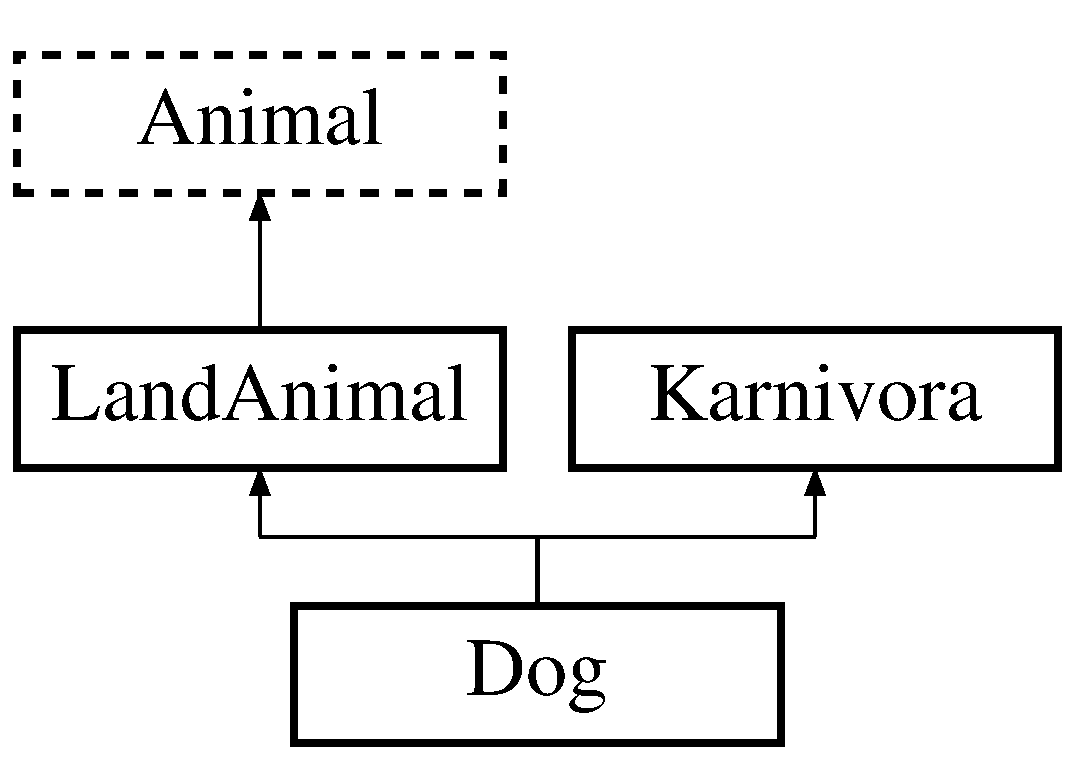
\includegraphics[height=3.000000cm]{classDog}
\end{center}
\end{figure}
\subsection*{Public Member Functions}
\begin{DoxyCompactItemize}
\item 
\hyperlink{classDog_afcf29443cf093c134c3d2febf307d831}{Dog} (int \-\_\-x, int \-\_\-y)
\begin{DoxyCompactList}\small\item\em Constructor. \end{DoxyCompactList}\item 
\hypertarget{classDog_aeacf410641eab28eabea6bc5269eb4ef}{\hyperlink{classDog_aeacf410641eab28eabea6bc5269eb4ef}{$\sim$\-Dog} ()}\label{classDog_aeacf410641eab28eabea6bc5269eb4ef}

\begin{DoxyCompactList}\small\item\em Destructor. \end{DoxyCompactList}\item 
\hypertarget{classDog_a843dea97bbe95afc6dc4692fcaeb757a}{void \hyperlink{classDog_a843dea97bbe95afc6dc4692fcaeb757a}{add\-Bobot} ()}\label{classDog_a843dea97bbe95afc6dc4692fcaeb757a}

\begin{DoxyCompactList}\small\item\em Menambahkan bobot satu satuan. \end{DoxyCompactList}\item 
int \hyperlink{classDog_ac115925dae59dd1640161c1a5b163bea}{get\-Bobot} ()
\begin{DoxyCompactList}\small\item\em Mendapatkan nilai bobot dari \hyperlink{classDog}{Dog}. \end{DoxyCompactList}\item 
char \hyperlink{classDog_a20ea4c8b525fe4610f614f4259029eaa}{get\-Simbol} ()
\begin{DoxyCompactList}\small\item\em Mendapatkan simbol dari \hyperlink{classDog}{Dog}. \end{DoxyCompactList}\item 
string \hyperlink{classDog_a0b476b766a08a8d43ee40ab96a4425ad}{get\-Musuh} (int i)
\begin{DoxyCompactList}\small\item\em Mendapatkan musuh ke i dari \hyperlink{classDog}{Dog} Musuh merupakan \hyperlink{classAnimal}{Animal} lain yang tidak bisa tinggal dalam satu kandang dengan \hyperlink{classDog}{Dog}. \end{DoxyCompactList}\item 
string \hyperlink{classDog_ae281395a2d8329b6abe3a2bc2c26bf5b}{interact} ()
\begin{DoxyCompactList}\small\item\em Mendapatkan reaksi \hyperlink{classDog}{Dog} saat berinteraksi dengan pengunjung. \end{DoxyCompactList}\item 
string \hyperlink{classDog_a3bc9048629f101f1aa7da5708ff1ef9a}{get\-Tipe\-Animal} ()
\begin{DoxyCompactList}\small\item\em Mendapatkan tipe \hyperlink{classAnimal}{Animal} (nama spesies) \end{DoxyCompactList}\end{DoxyCompactItemize}
\subsection*{Protected Attributes}
\begin{DoxyCompactItemize}
\item 
\hypertarget{classDog_af3d03f883e5c54c8426524a4bc4695ef}{const string {\bfseries tipe\-Animal} = \char`\"{}dog\char`\"{}}\label{classDog_af3d03f883e5c54c8426524a4bc4695ef}

\item 
\hypertarget{classDog_a754aaf1f196590ac3bd4411218dd02d9}{const char {\bfseries simbol} = 'd'}\label{classDog_a754aaf1f196590ac3bd4411218dd02d9}

\item 
\hypertarget{classDog_a6710ba8e06bc6afdd9eeaa28efa42c55}{int {\bfseries bobot}}\label{classDog_a6710ba8e06bc6afdd9eeaa28efa42c55}

\item 
\hypertarget{classDog_a0292ec8f9476757958127cb48abf40f4}{string $\ast$ {\bfseries musuh}}\label{classDog_a0292ec8f9476757958127cb48abf40f4}

\end{DoxyCompactItemize}


\subsection{Detailed Description}
Merupakan \hyperlink{classAnimal}{Animal} yang tinggal di darat dan merupakan \hyperlink{classKarnivora}{Karnivora} 

\subsection{Constructor \& Destructor Documentation}
\hypertarget{classDog_afcf29443cf093c134c3d2febf307d831}{\index{Dog@{Dog}!Dog@{Dog}}
\index{Dog@{Dog}!Dog@{Dog}}
\subsubsection[{Dog}]{\setlength{\rightskip}{0pt plus 5cm}Dog\-::\-Dog (
\begin{DoxyParamCaption}
\item[{int}]{\-\_\-x, }
\item[{int}]{\-\_\-y}
\end{DoxyParamCaption}
)}}\label{classDog_afcf29443cf093c134c3d2febf307d831}


Constructor. 


\begin{DoxyParams}{Parameters}
{\em \-\_\-x} & posisi x awal \hyperlink{classDog}{Dog} \\
\hline
{\em \-\_\-y} & posisi y awal \hyperlink{classDog}{Dog} \\
\hline
\end{DoxyParams}


\subsection{Member Function Documentation}
\hypertarget{classDog_ac115925dae59dd1640161c1a5b163bea}{\index{Dog@{Dog}!get\-Bobot@{get\-Bobot}}
\index{get\-Bobot@{get\-Bobot}!Dog@{Dog}}
\subsubsection[{get\-Bobot}]{\setlength{\rightskip}{0pt plus 5cm}int Dog\-::get\-Bobot (
\begin{DoxyParamCaption}
{}
\end{DoxyParamCaption}
)\hspace{0.3cm}{\ttfamily [virtual]}}}\label{classDog_ac115925dae59dd1640161c1a5b163bea}


Mendapatkan nilai bobot dari \hyperlink{classDog}{Dog}. 

\begin{DoxyReturn}{Returns}
bobot 
\end{DoxyReturn}


Implements \hyperlink{classAnimal}{Animal}.

\hypertarget{classDog_a0b476b766a08a8d43ee40ab96a4425ad}{\index{Dog@{Dog}!get\-Musuh@{get\-Musuh}}
\index{get\-Musuh@{get\-Musuh}!Dog@{Dog}}
\subsubsection[{get\-Musuh}]{\setlength{\rightskip}{0pt plus 5cm}string Dog\-::get\-Musuh (
\begin{DoxyParamCaption}
\item[{int}]{i}
\end{DoxyParamCaption}
)\hspace{0.3cm}{\ttfamily [virtual]}}}\label{classDog_a0b476b766a08a8d43ee40ab96a4425ad}


Mendapatkan musuh ke i dari \hyperlink{classDog}{Dog} Musuh merupakan \hyperlink{classAnimal}{Animal} lain yang tidak bisa tinggal dalam satu kandang dengan \hyperlink{classDog}{Dog}. 

\begin{DoxyReturn}{Returns}
musuh\mbox{[}i\mbox{]} 
\end{DoxyReturn}


Implements \hyperlink{classAnimal}{Animal}.

\hypertarget{classDog_a20ea4c8b525fe4610f614f4259029eaa}{\index{Dog@{Dog}!get\-Simbol@{get\-Simbol}}
\index{get\-Simbol@{get\-Simbol}!Dog@{Dog}}
\subsubsection[{get\-Simbol}]{\setlength{\rightskip}{0pt plus 5cm}char Dog\-::get\-Simbol (
\begin{DoxyParamCaption}
{}
\end{DoxyParamCaption}
)\hspace{0.3cm}{\ttfamily [virtual]}}}\label{classDog_a20ea4c8b525fe4610f614f4259029eaa}


Mendapatkan simbol dari \hyperlink{classDog}{Dog}. 

\begin{DoxyReturn}{Returns}
simbol 
\end{DoxyReturn}


Implements \hyperlink{classAnimal}{Animal}.

\hypertarget{classDog_a3bc9048629f101f1aa7da5708ff1ef9a}{\index{Dog@{Dog}!get\-Tipe\-Animal@{get\-Tipe\-Animal}}
\index{get\-Tipe\-Animal@{get\-Tipe\-Animal}!Dog@{Dog}}
\subsubsection[{get\-Tipe\-Animal}]{\setlength{\rightskip}{0pt plus 5cm}string Dog\-::get\-Tipe\-Animal (
\begin{DoxyParamCaption}
{}
\end{DoxyParamCaption}
)\hspace{0.3cm}{\ttfamily [virtual]}}}\label{classDog_a3bc9048629f101f1aa7da5708ff1ef9a}


Mendapatkan tipe \hyperlink{classAnimal}{Animal} (nama spesies) 

\begin{DoxyReturn}{Returns}
tipe\-Animal 
\end{DoxyReturn}


Implements \hyperlink{classLandAnimal}{Land\-Animal}.

\hypertarget{classDog_ae281395a2d8329b6abe3a2bc2c26bf5b}{\index{Dog@{Dog}!interact@{interact}}
\index{interact@{interact}!Dog@{Dog}}
\subsubsection[{interact}]{\setlength{\rightskip}{0pt plus 5cm}string Dog\-::interact (
\begin{DoxyParamCaption}
{}
\end{DoxyParamCaption}
)\hspace{0.3cm}{\ttfamily [virtual]}}}\label{classDog_ae281395a2d8329b6abe3a2bc2c26bf5b}


Mendapatkan reaksi \hyperlink{classDog}{Dog} saat berinteraksi dengan pengunjung. 

\begin{DoxyReturn}{Returns}
\char`\"{}barkbark\char`\"{} 
\end{DoxyReturn}


Implements \hyperlink{classLandAnimal}{Land\-Animal}.



The documentation for this class was generated from the following files\-:\begin{DoxyCompactItemize}
\item 
Dog.\-h\item 
Dog.\-cpp\end{DoxyCompactItemize}

\hypertarget{classDuck}{\section{Duck Class Reference}
\label{classDuck}\index{Duck@{Duck}}
}


{\ttfamily \#include $<$Duck.\-h$>$}

Inheritance diagram for Duck\-:\begin{figure}[H]
\begin{center}
\leavevmode
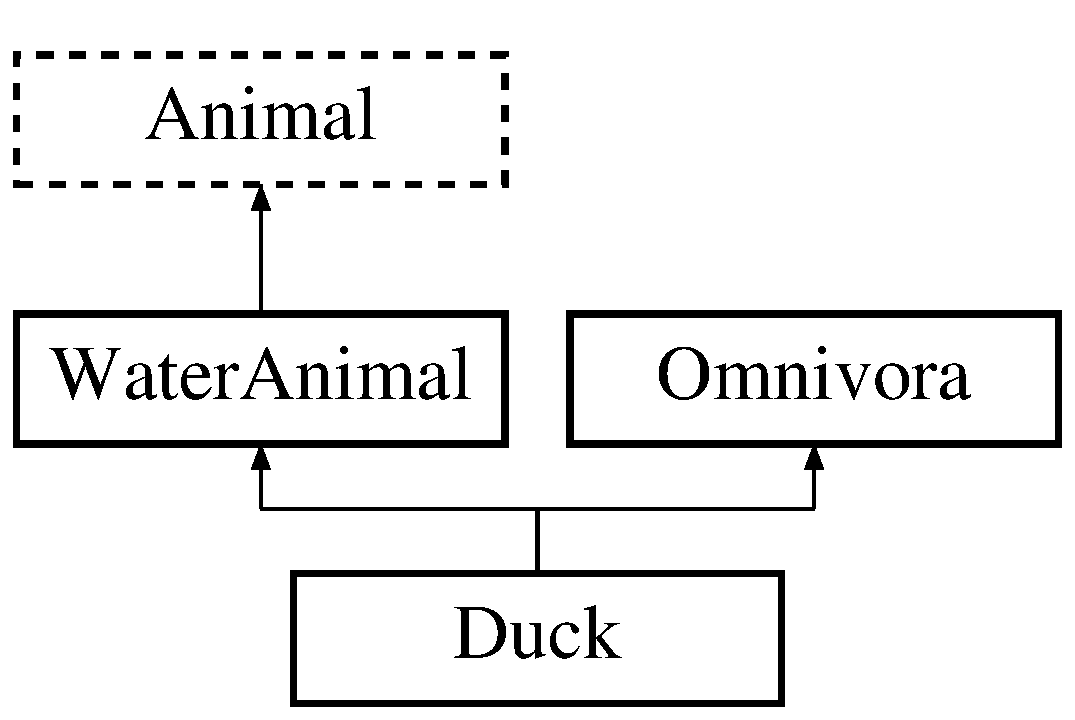
\includegraphics[height=3.000000cm]{classDuck}
\end{center}
\end{figure}
\subsection*{Public Member Functions}
\begin{DoxyCompactItemize}
\item 
\hyperlink{classDuck_a1322bd1a93555cd105e2496ba2de2a30}{Duck} (int \-\_\-x, int \-\_\-y)
\begin{DoxyCompactList}\small\item\em Constructor. \end{DoxyCompactList}\item 
\hypertarget{classDuck_a702222da0aa85e48b6ef945e9c53e68d}{\hyperlink{classDuck_a702222da0aa85e48b6ef945e9c53e68d}{$\sim$\-Duck} ()}\label{classDuck_a702222da0aa85e48b6ef945e9c53e68d}

\begin{DoxyCompactList}\small\item\em Destructor. \end{DoxyCompactList}\item 
\hypertarget{classDuck_ad0f24d52e0643275dfa7ab85838a174f}{void \hyperlink{classDuck_ad0f24d52e0643275dfa7ab85838a174f}{add\-Bobot} ()}\label{classDuck_ad0f24d52e0643275dfa7ab85838a174f}

\begin{DoxyCompactList}\small\item\em Menambahkan bobot satu satuan. \end{DoxyCompactList}\item 
int \hyperlink{classDuck_a21b1a913746b22e7cc50f00821605cf2}{get\-Bobot} ()
\begin{DoxyCompactList}\small\item\em Mendapatkan nilai bobot dari \hyperlink{classDuck}{Duck}. \end{DoxyCompactList}\item 
char \hyperlink{classDuck_a96b13b494232f7d4bffbce7eec321d87}{get\-Simbol} ()
\begin{DoxyCompactList}\small\item\em Mendapatkan simbol dari \hyperlink{classDuck}{Duck}. \end{DoxyCompactList}\item 
string \hyperlink{classDuck_a2b3f2c06edc5558de242bb3df9564525}{get\-Musuh} (int i)
\begin{DoxyCompactList}\small\item\em Mendapatkan musuh ke i dari \hyperlink{classDuck}{Duck} Musuh merupakan \hyperlink{classAnimal}{Animal} lain yang tidak bisa tinggal dalam satu kandang dengan \hyperlink{classDuck}{Duck}. \end{DoxyCompactList}\item 
string \hyperlink{classDuck_a2a8991eb931ec90eef13b9e4ead8f219}{interact} ()
\begin{DoxyCompactList}\small\item\em Mendapatkan reaksi \hyperlink{classDuck}{Duck} saat berinteraksi dengan pengunjung. \end{DoxyCompactList}\item 
string \hyperlink{classDuck_a9677d398bea572e67d908a0fe32bde9a}{get\-Tipe\-Animal} ()
\begin{DoxyCompactList}\small\item\em Mendapatkan tipe \hyperlink{classAnimal}{Animal} (nama spesies) \end{DoxyCompactList}\end{DoxyCompactItemize}
\subsection*{Protected Attributes}
\begin{DoxyCompactItemize}
\item 
\hypertarget{classDuck_a0c747e97b8a811278efa65ede9b109bf}{const string {\bfseries tipe\-Animal} = \char`\"{}duck\char`\"{}}\label{classDuck_a0c747e97b8a811278efa65ede9b109bf}

\item 
\hypertarget{classDuck_a521348676043da1fa5b4c4ec63428913}{const char {\bfseries simbol} = 'k'}\label{classDuck_a521348676043da1fa5b4c4ec63428913}

\item 
\hypertarget{classDuck_a5e195f611176415ad510a20d9fa2a91c}{int {\bfseries bobot}}\label{classDuck_a5e195f611176415ad510a20d9fa2a91c}

\item 
\hypertarget{classDuck_a56988b05f48c2c1efadc04d4bcb41ed9}{string $\ast$ {\bfseries musuh}}\label{classDuck_a56988b05f48c2c1efadc04d4bcb41ed9}

\end{DoxyCompactItemize}


\subsection{Detailed Description}
Merupakan \hyperlink{classAnimal}{Animal} yang tinggal di air dan merupakan \hyperlink{classOmnivora}{Omnivora} 

\subsection{Constructor \& Destructor Documentation}
\hypertarget{classDuck_a1322bd1a93555cd105e2496ba2de2a30}{\index{Duck@{Duck}!Duck@{Duck}}
\index{Duck@{Duck}!Duck@{Duck}}
\subsubsection[{Duck}]{\setlength{\rightskip}{0pt plus 5cm}Duck\-::\-Duck (
\begin{DoxyParamCaption}
\item[{int}]{\-\_\-x, }
\item[{int}]{\-\_\-y}
\end{DoxyParamCaption}
)}}\label{classDuck_a1322bd1a93555cd105e2496ba2de2a30}


Constructor. 


\begin{DoxyParams}{Parameters}
{\em \-\_\-x} & posisi x awal \hyperlink{classDuck}{Duck} \\
\hline
{\em \-\_\-y} & posisi y awal \hyperlink{classDuck}{Duck} \\
\hline
\end{DoxyParams}


\subsection{Member Function Documentation}
\hypertarget{classDuck_a21b1a913746b22e7cc50f00821605cf2}{\index{Duck@{Duck}!get\-Bobot@{get\-Bobot}}
\index{get\-Bobot@{get\-Bobot}!Duck@{Duck}}
\subsubsection[{get\-Bobot}]{\setlength{\rightskip}{0pt plus 5cm}int Duck\-::get\-Bobot (
\begin{DoxyParamCaption}
{}
\end{DoxyParamCaption}
)\hspace{0.3cm}{\ttfamily [virtual]}}}\label{classDuck_a21b1a913746b22e7cc50f00821605cf2}


Mendapatkan nilai bobot dari \hyperlink{classDuck}{Duck}. 

\begin{DoxyReturn}{Returns}
bobot 
\end{DoxyReturn}


Implements \hyperlink{classAnimal}{Animal}.

\hypertarget{classDuck_a2b3f2c06edc5558de242bb3df9564525}{\index{Duck@{Duck}!get\-Musuh@{get\-Musuh}}
\index{get\-Musuh@{get\-Musuh}!Duck@{Duck}}
\subsubsection[{get\-Musuh}]{\setlength{\rightskip}{0pt plus 5cm}string Duck\-::get\-Musuh (
\begin{DoxyParamCaption}
\item[{int}]{i}
\end{DoxyParamCaption}
)\hspace{0.3cm}{\ttfamily [virtual]}}}\label{classDuck_a2b3f2c06edc5558de242bb3df9564525}


Mendapatkan musuh ke i dari \hyperlink{classDuck}{Duck} Musuh merupakan \hyperlink{classAnimal}{Animal} lain yang tidak bisa tinggal dalam satu kandang dengan \hyperlink{classDuck}{Duck}. 

\begin{DoxyReturn}{Returns}
musuh\mbox{[}i\mbox{]} 
\end{DoxyReturn}


Implements \hyperlink{classAnimal}{Animal}.

\hypertarget{classDuck_a96b13b494232f7d4bffbce7eec321d87}{\index{Duck@{Duck}!get\-Simbol@{get\-Simbol}}
\index{get\-Simbol@{get\-Simbol}!Duck@{Duck}}
\subsubsection[{get\-Simbol}]{\setlength{\rightskip}{0pt plus 5cm}char Duck\-::get\-Simbol (
\begin{DoxyParamCaption}
{}
\end{DoxyParamCaption}
)\hspace{0.3cm}{\ttfamily [virtual]}}}\label{classDuck_a96b13b494232f7d4bffbce7eec321d87}


Mendapatkan simbol dari \hyperlink{classDuck}{Duck}. 

\begin{DoxyReturn}{Returns}
simbol 
\end{DoxyReturn}


Implements \hyperlink{classAnimal}{Animal}.

\hypertarget{classDuck_a9677d398bea572e67d908a0fe32bde9a}{\index{Duck@{Duck}!get\-Tipe\-Animal@{get\-Tipe\-Animal}}
\index{get\-Tipe\-Animal@{get\-Tipe\-Animal}!Duck@{Duck}}
\subsubsection[{get\-Tipe\-Animal}]{\setlength{\rightskip}{0pt plus 5cm}string Duck\-::get\-Tipe\-Animal (
\begin{DoxyParamCaption}
{}
\end{DoxyParamCaption}
)\hspace{0.3cm}{\ttfamily [virtual]}}}\label{classDuck_a9677d398bea572e67d908a0fe32bde9a}


Mendapatkan tipe \hyperlink{classAnimal}{Animal} (nama spesies) 

\begin{DoxyReturn}{Returns}
tipe\-Animal 
\end{DoxyReturn}


Implements \hyperlink{classWaterAnimal}{Water\-Animal}.

\hypertarget{classDuck_a2a8991eb931ec90eef13b9e4ead8f219}{\index{Duck@{Duck}!interact@{interact}}
\index{interact@{interact}!Duck@{Duck}}
\subsubsection[{interact}]{\setlength{\rightskip}{0pt plus 5cm}string Duck\-::interact (
\begin{DoxyParamCaption}
{}
\end{DoxyParamCaption}
)\hspace{0.3cm}{\ttfamily [virtual]}}}\label{classDuck_a2a8991eb931ec90eef13b9e4ead8f219}


Mendapatkan reaksi \hyperlink{classDuck}{Duck} saat berinteraksi dengan pengunjung. 

\begin{DoxyReturn}{Returns}
\char`\"{}kwekwek\char`\"{} 
\end{DoxyReturn}


Implements \hyperlink{classWaterAnimal}{Water\-Animal}.



The documentation for this class was generated from the following files\-:\begin{DoxyCompactItemize}
\item 
Duck.\-h\item 
Duck.\-cpp\end{DoxyCompactItemize}

\hypertarget{classEagle}{\section{Eagle Class Reference}
\label{classEagle}\index{Eagle@{Eagle}}
}


{\ttfamily \#include $<$Eagle.\-h$>$}

Inheritance diagram for Eagle\-:\begin{figure}[H]
\begin{center}
\leavevmode
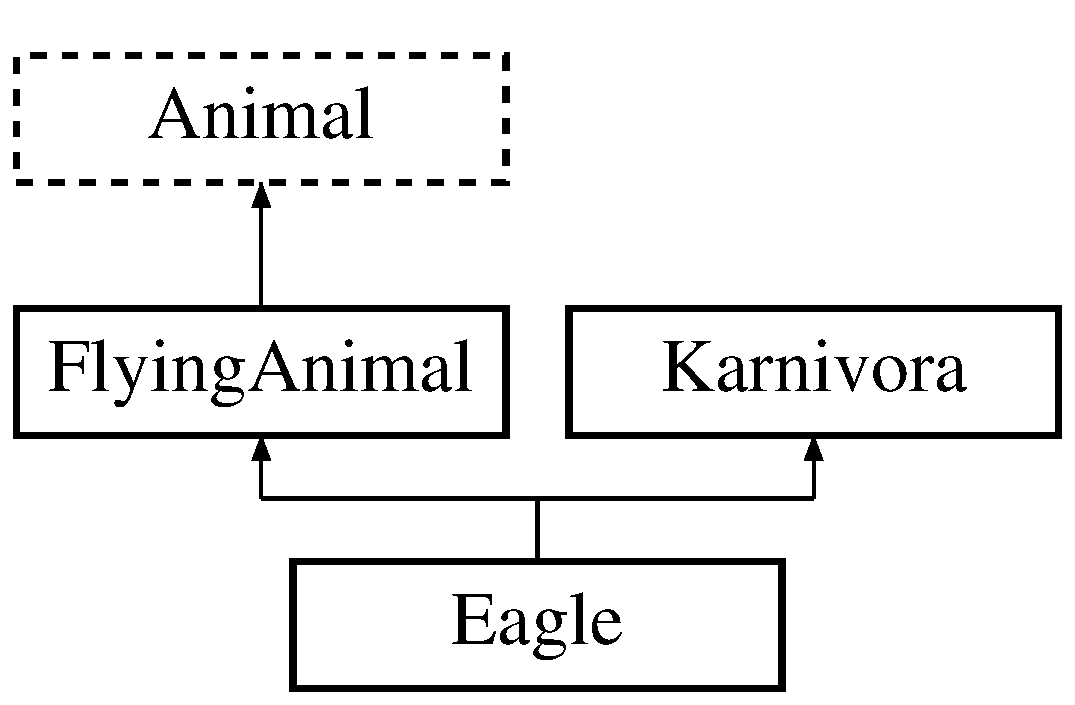
\includegraphics[height=3.000000cm]{classEagle}
\end{center}
\end{figure}
\subsection*{Public Member Functions}
\begin{DoxyCompactItemize}
\item 
\hyperlink{classEagle_abcdafbd20745ef82b612ca4839f221ec}{Eagle} (int \-\_\-x, int \-\_\-y)
\begin{DoxyCompactList}\small\item\em Constructor. \end{DoxyCompactList}\item 
\hypertarget{classEagle_a192a898182736506c1f78159bf3477b7}{\hyperlink{classEagle_a192a898182736506c1f78159bf3477b7}{$\sim$\-Eagle} ()}\label{classEagle_a192a898182736506c1f78159bf3477b7}

\begin{DoxyCompactList}\small\item\em Destructor. \end{DoxyCompactList}\item 
\hypertarget{classEagle_a59a6326f2e7a63a1d0d724d37402652d}{void \hyperlink{classEagle_a59a6326f2e7a63a1d0d724d37402652d}{add\-Bobot} ()}\label{classEagle_a59a6326f2e7a63a1d0d724d37402652d}

\begin{DoxyCompactList}\small\item\em Menambahkan bobot satu satuasn. \end{DoxyCompactList}\item 
int \hyperlink{classEagle_a15ec50591c567e370b8b5811ea3724c9}{get\-Bobot} ()
\begin{DoxyCompactList}\small\item\em Mendapatkan nilai bobot dari \hyperlink{classEagle}{Eagle}. \end{DoxyCompactList}\item 
char \hyperlink{classEagle_a4f15b35b579496054a80f6bf9ac5e4f8}{get\-Simbol} ()
\begin{DoxyCompactList}\small\item\em Mendapatkan simbol dari \hyperlink{classEagle}{Eagle}. \end{DoxyCompactList}\item 
string \hyperlink{classEagle_ab0082d6c81ae02d38cf87ffd8844b1f6}{get\-Musuh} (int i)
\begin{DoxyCompactList}\small\item\em Mendapatkan musuh ke i dari \hyperlink{classEagle}{Eagle} Musuh merupakan \hyperlink{classAnimal}{Animal} lain yang tidak bisa tinggal dalam satu kandang dengan \hyperlink{classEagle}{Eagle}. \end{DoxyCompactList}\item 
string \hyperlink{classEagle_a698f925269924e7e9f9b9c92899de01d}{interact} ()
\begin{DoxyCompactList}\small\item\em Mendapatkan reaksi \hyperlink{classEagle}{Eagle} saat berinteraksi dengan pengunjung. \end{DoxyCompactList}\item 
string \hyperlink{classEagle_af9d6c21fd2e046487b3490bb12ad3d6e}{get\-Tipe\-Animal} ()
\begin{DoxyCompactList}\small\item\em Mendapatkan tipe \hyperlink{classAnimal}{Animal} (nama spesies) \end{DoxyCompactList}\end{DoxyCompactItemize}
\subsection*{Protected Attributes}
\begin{DoxyCompactItemize}
\item 
\hypertarget{classEagle_a9bd67850db91066aa7721cefea7dcd77}{const string {\bfseries tipe\-Animal} = \char`\"{}eagle\char`\"{}}\label{classEagle_a9bd67850db91066aa7721cefea7dcd77}

\item 
\hypertarget{classEagle_af8fe332fc3ea5bc279fb097feafcc4e2}{const char {\bfseries simbol} = 'a'}\label{classEagle_af8fe332fc3ea5bc279fb097feafcc4e2}

\item 
\hypertarget{classEagle_a87a653ea21dbca9c25ec0108a173e879}{int {\bfseries bobot}}\label{classEagle_a87a653ea21dbca9c25ec0108a173e879}

\item 
\hypertarget{classEagle_a76c2afa3a70eeb14ceb5733f4b26da4b}{string $\ast$ {\bfseries musuh}}\label{classEagle_a76c2afa3a70eeb14ceb5733f4b26da4b}

\end{DoxyCompactItemize}


\subsection{Detailed Description}
Merupakan \hyperlink{classAnimal}{Animal} yang tinggal di udara dan merupakan \hyperlink{classKarnivora}{Karnivora} 

\subsection{Constructor \& Destructor Documentation}
\hypertarget{classEagle_abcdafbd20745ef82b612ca4839f221ec}{\index{Eagle@{Eagle}!Eagle@{Eagle}}
\index{Eagle@{Eagle}!Eagle@{Eagle}}
\subsubsection[{Eagle}]{\setlength{\rightskip}{0pt plus 5cm}Eagle\-::\-Eagle (
\begin{DoxyParamCaption}
\item[{int}]{\-\_\-x, }
\item[{int}]{\-\_\-y}
\end{DoxyParamCaption}
)}}\label{classEagle_abcdafbd20745ef82b612ca4839f221ec}


Constructor. 


\begin{DoxyParams}{Parameters}
{\em \-\_\-x} & posisi x awal \hyperlink{classEagle}{Eagle} \\
\hline
{\em \-\_\-y} & posisi y awal \hyperlink{classEagle}{Eagle} \\
\hline
\end{DoxyParams}


\subsection{Member Function Documentation}
\hypertarget{classEagle_a15ec50591c567e370b8b5811ea3724c9}{\index{Eagle@{Eagle}!get\-Bobot@{get\-Bobot}}
\index{get\-Bobot@{get\-Bobot}!Eagle@{Eagle}}
\subsubsection[{get\-Bobot}]{\setlength{\rightskip}{0pt plus 5cm}int Eagle\-::get\-Bobot (
\begin{DoxyParamCaption}
{}
\end{DoxyParamCaption}
)\hspace{0.3cm}{\ttfamily [virtual]}}}\label{classEagle_a15ec50591c567e370b8b5811ea3724c9}


Mendapatkan nilai bobot dari \hyperlink{classEagle}{Eagle}. 

\begin{DoxyReturn}{Returns}
bobot 
\end{DoxyReturn}


Implements \hyperlink{classAnimal}{Animal}.

\hypertarget{classEagle_ab0082d6c81ae02d38cf87ffd8844b1f6}{\index{Eagle@{Eagle}!get\-Musuh@{get\-Musuh}}
\index{get\-Musuh@{get\-Musuh}!Eagle@{Eagle}}
\subsubsection[{get\-Musuh}]{\setlength{\rightskip}{0pt plus 5cm}string Eagle\-::get\-Musuh (
\begin{DoxyParamCaption}
\item[{int}]{i}
\end{DoxyParamCaption}
)\hspace{0.3cm}{\ttfamily [virtual]}}}\label{classEagle_ab0082d6c81ae02d38cf87ffd8844b1f6}


Mendapatkan musuh ke i dari \hyperlink{classEagle}{Eagle} Musuh merupakan \hyperlink{classAnimal}{Animal} lain yang tidak bisa tinggal dalam satu kandang dengan \hyperlink{classEagle}{Eagle}. 

\begin{DoxyReturn}{Returns}
musuh\mbox{[}i\mbox{]} 
\end{DoxyReturn}


Implements \hyperlink{classAnimal}{Animal}.

\hypertarget{classEagle_a4f15b35b579496054a80f6bf9ac5e4f8}{\index{Eagle@{Eagle}!get\-Simbol@{get\-Simbol}}
\index{get\-Simbol@{get\-Simbol}!Eagle@{Eagle}}
\subsubsection[{get\-Simbol}]{\setlength{\rightskip}{0pt plus 5cm}char Eagle\-::get\-Simbol (
\begin{DoxyParamCaption}
{}
\end{DoxyParamCaption}
)\hspace{0.3cm}{\ttfamily [virtual]}}}\label{classEagle_a4f15b35b579496054a80f6bf9ac5e4f8}


Mendapatkan simbol dari \hyperlink{classEagle}{Eagle}. 

\begin{DoxyReturn}{Returns}
simbol 
\end{DoxyReturn}


Implements \hyperlink{classAnimal}{Animal}.

\hypertarget{classEagle_af9d6c21fd2e046487b3490bb12ad3d6e}{\index{Eagle@{Eagle}!get\-Tipe\-Animal@{get\-Tipe\-Animal}}
\index{get\-Tipe\-Animal@{get\-Tipe\-Animal}!Eagle@{Eagle}}
\subsubsection[{get\-Tipe\-Animal}]{\setlength{\rightskip}{0pt plus 5cm}string Eagle\-::get\-Tipe\-Animal (
\begin{DoxyParamCaption}
{}
\end{DoxyParamCaption}
)\hspace{0.3cm}{\ttfamily [virtual]}}}\label{classEagle_af9d6c21fd2e046487b3490bb12ad3d6e}


Mendapatkan tipe \hyperlink{classAnimal}{Animal} (nama spesies) 

\begin{DoxyReturn}{Returns}
tipe\-Animal 
\end{DoxyReturn}


Implements \hyperlink{classFlyingAnimal_a1523973b9a6a47e9064825c2134fd65d}{Flying\-Animal}.

\hypertarget{classEagle_a698f925269924e7e9f9b9c92899de01d}{\index{Eagle@{Eagle}!interact@{interact}}
\index{interact@{interact}!Eagle@{Eagle}}
\subsubsection[{interact}]{\setlength{\rightskip}{0pt plus 5cm}string Eagle\-::interact (
\begin{DoxyParamCaption}
{}
\end{DoxyParamCaption}
)\hspace{0.3cm}{\ttfamily [virtual]}}}\label{classEagle_a698f925269924e7e9f9b9c92899de01d}


Mendapatkan reaksi \hyperlink{classEagle}{Eagle} saat berinteraksi dengan pengunjung. 

\begin{DoxyReturn}{Returns}
\char`\"{}gakgak\char`\"{} 
\end{DoxyReturn}


Implements \hyperlink{classFlyingAnimal_ac0eee625fa2235eee8cbdc0a010ae430}{Flying\-Animal}.



The documentation for this class was generated from the following files\-:\begin{DoxyCompactItemize}
\item 
Eagle.\-h\item 
Eagle.\-cpp\end{DoxyCompactItemize}

\hypertarget{classElephant}{\section{Elephant Class Reference}
\label{classElephant}\index{Elephant@{Elephant}}
}
Inheritance diagram for Elephant\-:\begin{figure}[H]
\begin{center}
\leavevmode
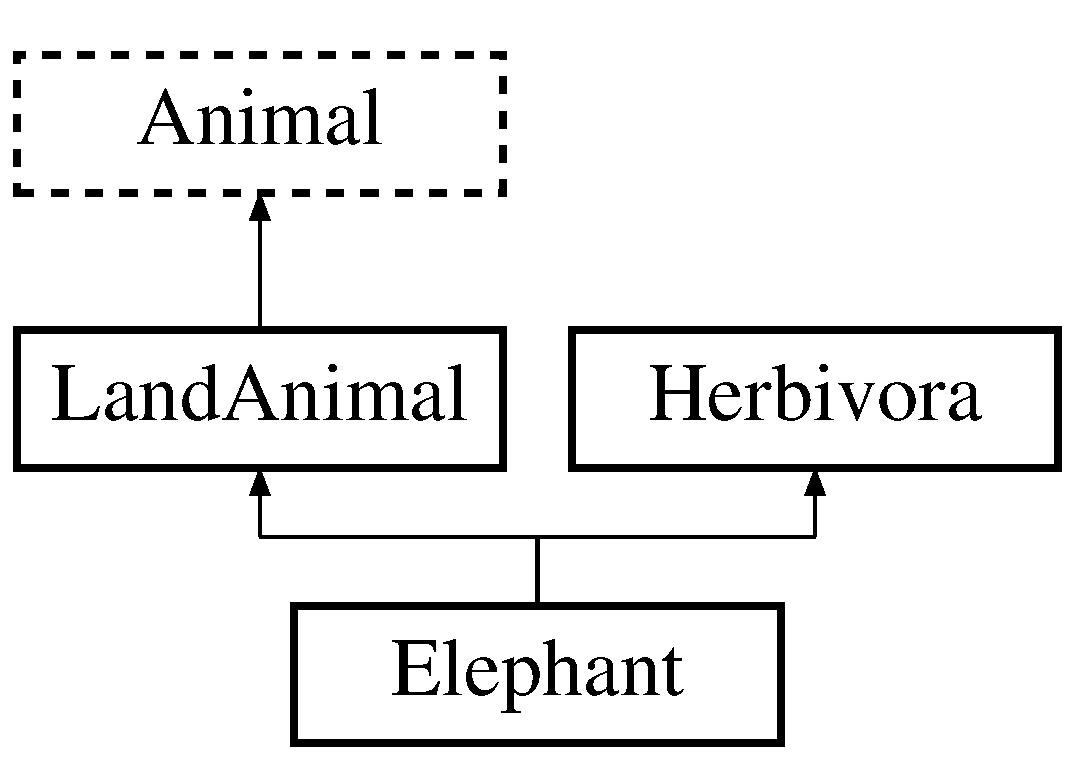
\includegraphics[height=3.000000cm]{classElephant}
\end{center}
\end{figure}
\subsection*{Public Member Functions}
\begin{DoxyCompactItemize}
\item 
\hyperlink{classElephant_a581d01caaa767f869ebb68c1d9e6017b}{Elephant} (int \-\_\-x, int \-\_\-y)
\begin{DoxyCompactList}\small\item\em Constructor. \end{DoxyCompactList}\item 
\hypertarget{classElephant_a8f290b4b7acfed8f2f23bab9326ece3f}{\hyperlink{classElephant_a8f290b4b7acfed8f2f23bab9326ece3f}{$\sim$\-Elephant} ()}\label{classElephant_a8f290b4b7acfed8f2f23bab9326ece3f}

\begin{DoxyCompactList}\small\item\em Destructor. \end{DoxyCompactList}\item 
\hypertarget{classElephant_afafffb9d73c45d0100e15ec9c6c914a9}{void \hyperlink{classElephant_afafffb9d73c45d0100e15ec9c6c914a9}{add\-Bobot} ()}\label{classElephant_afafffb9d73c45d0100e15ec9c6c914a9}

\begin{DoxyCompactList}\small\item\em Menambahkan bobot satu satuan. \end{DoxyCompactList}\item 
int \hyperlink{classElephant_a662842931e97fa17fc67a37af92f88b8}{get\-Bobot} ()
\begin{DoxyCompactList}\small\item\em Mendapatkan nilai bobot dari \hyperlink{classSnake}{Snake}. \end{DoxyCompactList}\item 
char \hyperlink{classElephant_afb716b804efc9b33578f06aa875cdd4c}{get\-Simbol} ()
\begin{DoxyCompactList}\small\item\em Mendapatkan simbol dari \hyperlink{classSnake}{Snake}. \end{DoxyCompactList}\item 
string \hyperlink{classElephant_a6b033833b5b37942d965580ab901e735}{get\-Musuh} (int i)
\begin{DoxyCompactList}\small\item\em Mendapatkan musuh ke i dari \hyperlink{classSnake}{Snake} Musuh merupakan \hyperlink{classAnimal}{Animal} lain yang tidak bisa tinggal dalam satu kandang dengan \hyperlink{classSnake}{Snake}. \end{DoxyCompactList}\item 
string \hyperlink{classElephant_a321f653cd862265373e9c8985d683b3c}{interact} ()
\begin{DoxyCompactList}\small\item\em Mendapatkan reaksi \hyperlink{classSnake}{Snake} saat berinteraksi dengan pengunjung. \end{DoxyCompactList}\item 
string \hyperlink{classElephant_ae8964770f0b50674428e8b7f1041b86e}{get\-Tipe\-Animal} ()
\begin{DoxyCompactList}\small\item\em Mendapatkan tipe \hyperlink{classAnimal}{Animal} (nama spesies) \end{DoxyCompactList}\end{DoxyCompactItemize}
\subsection*{Protected Attributes}
\begin{DoxyCompactItemize}
\item 
\hypertarget{classElephant_aa80dde45853d4b749672e33c9978d235}{const string {\bfseries tipe\-Animal} = \char`\"{}elephant\char`\"{}}\label{classElephant_aa80dde45853d4b749672e33c9978d235}

\item 
\hypertarget{classElephant_adbb0e7e3cbf8321a9a74bc039163f1f3}{const char {\bfseries simbol} = 'e'}\label{classElephant_adbb0e7e3cbf8321a9a74bc039163f1f3}

\item 
\hypertarget{classElephant_ad6e7e6be15ba76d55eb990d98ff9f338}{int {\bfseries bobot}}\label{classElephant_ad6e7e6be15ba76d55eb990d98ff9f338}

\item 
\hypertarget{classElephant_acf18c4e3c369af5d606f3f82dca7fe4f}{string $\ast$ {\bfseries musuh}}\label{classElephant_acf18c4e3c369af5d606f3f82dca7fe4f}

\end{DoxyCompactItemize}


\subsection{Constructor \& Destructor Documentation}
\hypertarget{classElephant_a581d01caaa767f869ebb68c1d9e6017b}{\index{Elephant@{Elephant}!Elephant@{Elephant}}
\index{Elephant@{Elephant}!Elephant@{Elephant}}
\subsubsection[{Elephant}]{\setlength{\rightskip}{0pt plus 5cm}Elephant\-::\-Elephant (
\begin{DoxyParamCaption}
\item[{int}]{\-\_\-x, }
\item[{int}]{\-\_\-y}
\end{DoxyParamCaption}
)}}\label{classElephant_a581d01caaa767f869ebb68c1d9e6017b}


Constructor. 


\begin{DoxyParams}{Parameters}
{\em \-\_\-x} & posisi x awal \hyperlink{classSnake}{Snake} \\
\hline
{\em \-\_\-y} & posisi y awal \hyperlink{classSnake}{Snake} \\
\hline
\end{DoxyParams}


\subsection{Member Function Documentation}
\hypertarget{classElephant_a662842931e97fa17fc67a37af92f88b8}{\index{Elephant@{Elephant}!get\-Bobot@{get\-Bobot}}
\index{get\-Bobot@{get\-Bobot}!Elephant@{Elephant}}
\subsubsection[{get\-Bobot}]{\setlength{\rightskip}{0pt plus 5cm}int Elephant\-::get\-Bobot (
\begin{DoxyParamCaption}
{}
\end{DoxyParamCaption}
)\hspace{0.3cm}{\ttfamily [virtual]}}}\label{classElephant_a662842931e97fa17fc67a37af92f88b8}


Mendapatkan nilai bobot dari \hyperlink{classSnake}{Snake}. 

\begin{DoxyReturn}{Returns}
bobot 
\end{DoxyReturn}


Implements \hyperlink{classAnimal}{Animal}.

\hypertarget{classElephant_a6b033833b5b37942d965580ab901e735}{\index{Elephant@{Elephant}!get\-Musuh@{get\-Musuh}}
\index{get\-Musuh@{get\-Musuh}!Elephant@{Elephant}}
\subsubsection[{get\-Musuh}]{\setlength{\rightskip}{0pt plus 5cm}string Elephant\-::get\-Musuh (
\begin{DoxyParamCaption}
\item[{int}]{i}
\end{DoxyParamCaption}
)\hspace{0.3cm}{\ttfamily [virtual]}}}\label{classElephant_a6b033833b5b37942d965580ab901e735}


Mendapatkan musuh ke i dari \hyperlink{classSnake}{Snake} Musuh merupakan \hyperlink{classAnimal}{Animal} lain yang tidak bisa tinggal dalam satu kandang dengan \hyperlink{classSnake}{Snake}. 

\begin{DoxyReturn}{Returns}
musuh\mbox{[}i\mbox{]} 
\end{DoxyReturn}


Implements \hyperlink{classAnimal}{Animal}.

\hypertarget{classElephant_afb716b804efc9b33578f06aa875cdd4c}{\index{Elephant@{Elephant}!get\-Simbol@{get\-Simbol}}
\index{get\-Simbol@{get\-Simbol}!Elephant@{Elephant}}
\subsubsection[{get\-Simbol}]{\setlength{\rightskip}{0pt plus 5cm}char Elephant\-::get\-Simbol (
\begin{DoxyParamCaption}
{}
\end{DoxyParamCaption}
)\hspace{0.3cm}{\ttfamily [virtual]}}}\label{classElephant_afb716b804efc9b33578f06aa875cdd4c}


Mendapatkan simbol dari \hyperlink{classSnake}{Snake}. 

\begin{DoxyReturn}{Returns}
simbol 
\end{DoxyReturn}


Implements \hyperlink{classAnimal}{Animal}.

\hypertarget{classElephant_ae8964770f0b50674428e8b7f1041b86e}{\index{Elephant@{Elephant}!get\-Tipe\-Animal@{get\-Tipe\-Animal}}
\index{get\-Tipe\-Animal@{get\-Tipe\-Animal}!Elephant@{Elephant}}
\subsubsection[{get\-Tipe\-Animal}]{\setlength{\rightskip}{0pt plus 5cm}string Elephant\-::get\-Tipe\-Animal (
\begin{DoxyParamCaption}
{}
\end{DoxyParamCaption}
)\hspace{0.3cm}{\ttfamily [virtual]}}}\label{classElephant_ae8964770f0b50674428e8b7f1041b86e}


Mendapatkan tipe \hyperlink{classAnimal}{Animal} (nama spesies) 

\begin{DoxyReturn}{Returns}
tipe\-Animal 
\end{DoxyReturn}


Implements \hyperlink{classLandAnimal}{Land\-Animal}.

\hypertarget{classElephant_a321f653cd862265373e9c8985d683b3c}{\index{Elephant@{Elephant}!interact@{interact}}
\index{interact@{interact}!Elephant@{Elephant}}
\subsubsection[{interact}]{\setlength{\rightskip}{0pt plus 5cm}string Elephant\-::interact (
\begin{DoxyParamCaption}
{}
\end{DoxyParamCaption}
)\hspace{0.3cm}{\ttfamily [virtual]}}}\label{classElephant_a321f653cd862265373e9c8985d683b3c}


Mendapatkan reaksi \hyperlink{classSnake}{Snake} saat berinteraksi dengan pengunjung. 

\begin{DoxyReturn}{Returns}
\char`\"{}belalaihuee\char`\"{} 
\end{DoxyReturn}


Implements \hyperlink{classLandAnimal}{Land\-Animal}.



The documentation for this class was generated from the following files\-:\begin{DoxyCompactItemize}
\item 
Elephant.\-h\item 
Elephant.\-cpp\end{DoxyCompactItemize}

\hypertarget{classEntrance}{\section{Entrance Class Reference}
\label{classEntrance}\index{Entrance@{Entrance}}
}


{\ttfamily \#include $<$Entrance.\-h$>$}

Inheritance diagram for Entrance\-:\begin{figure}[H]
\begin{center}
\leavevmode
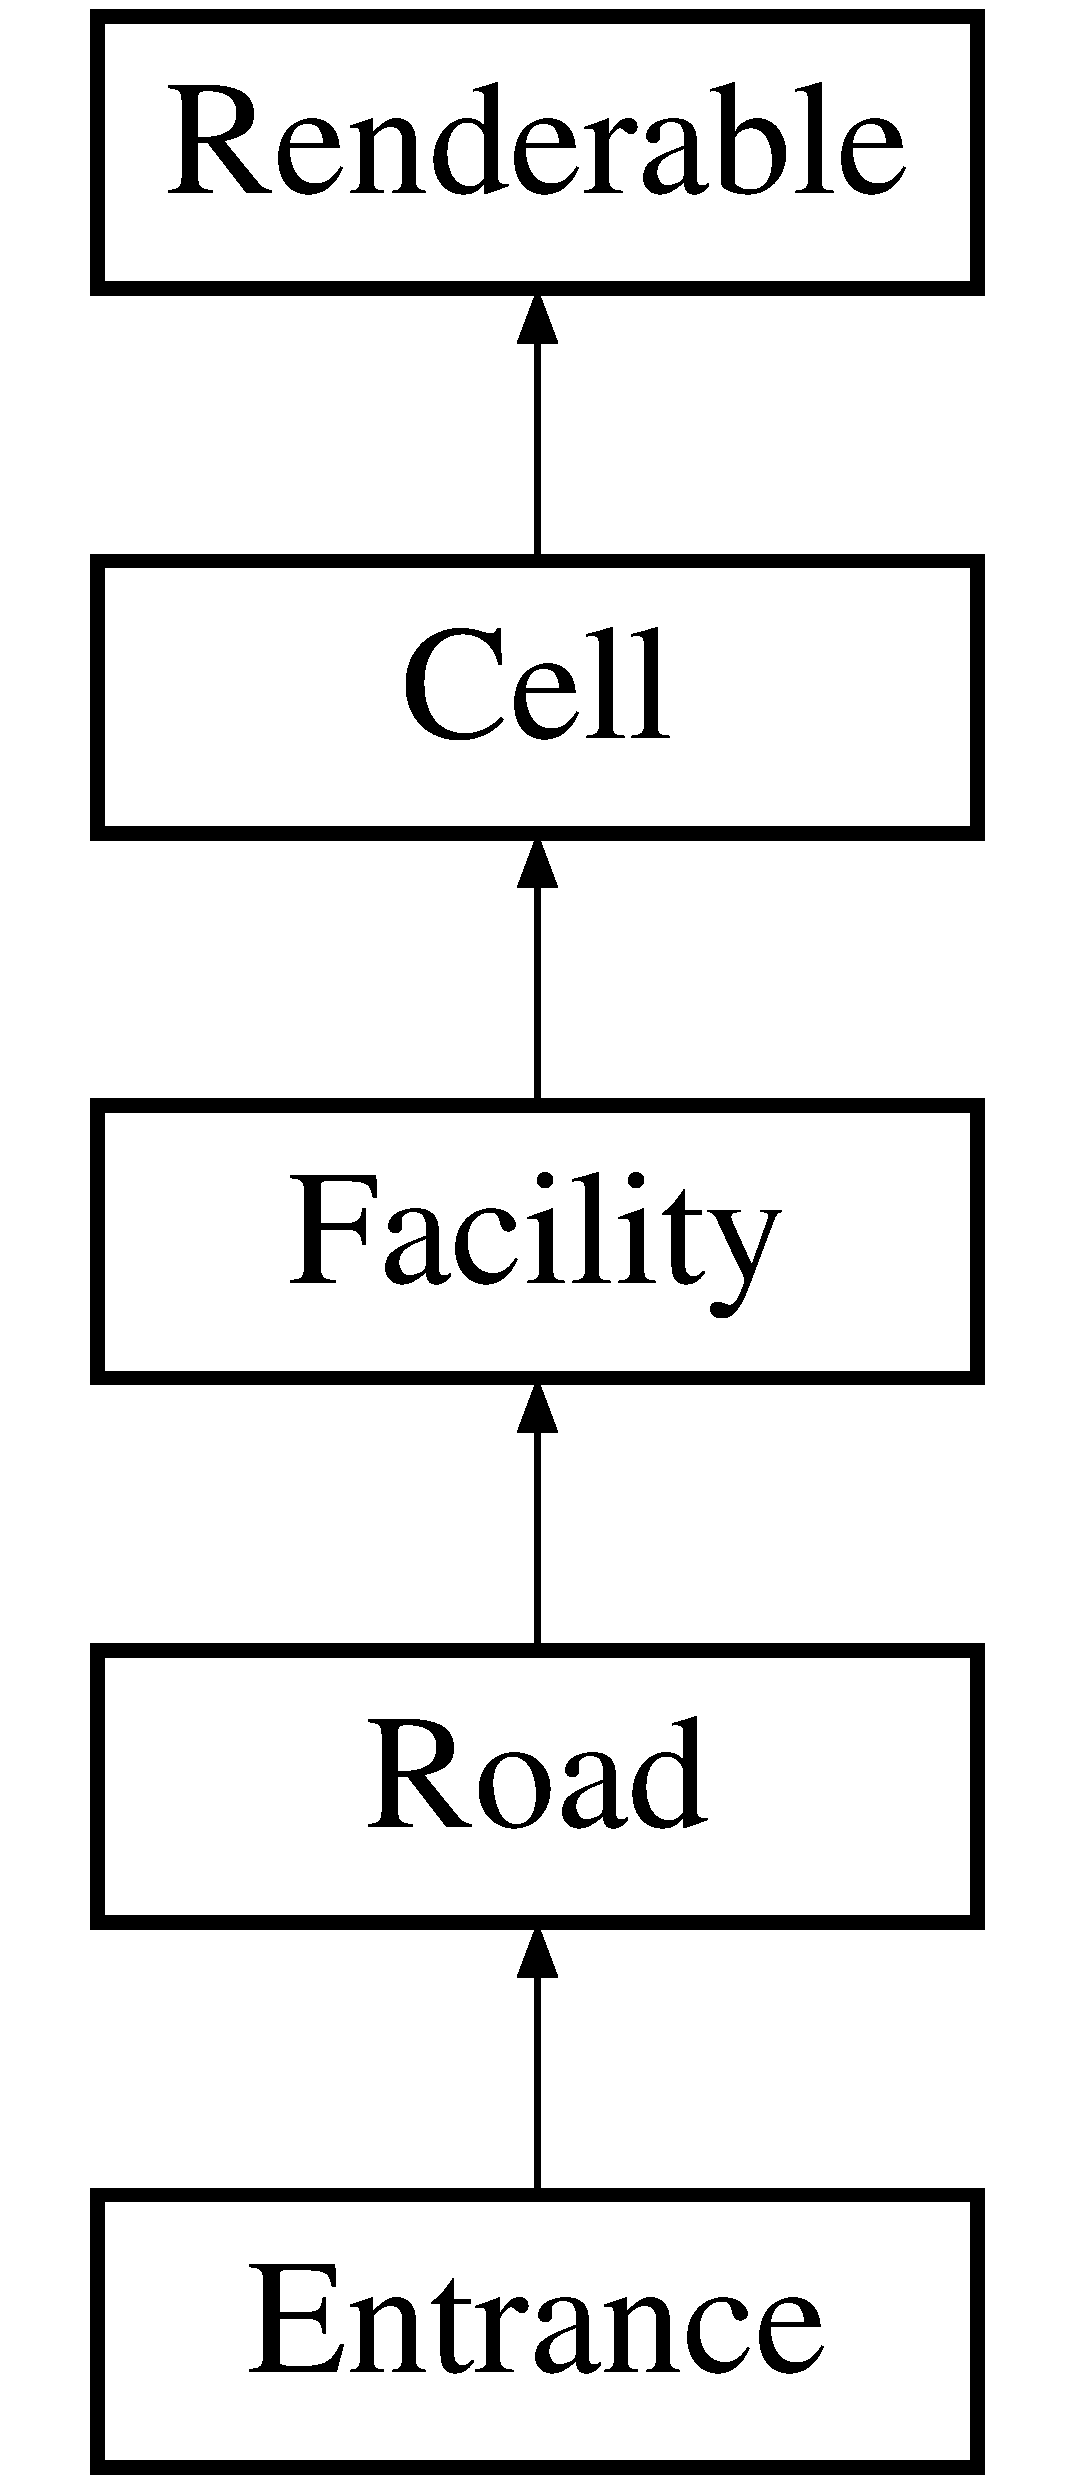
\includegraphics[height=5.000000cm]{classEntrance}
\end{center}
\end{figure}
\subsection*{Public Member Functions}
\begin{DoxyCompactItemize}
\item 
\hyperlink{classEntrance_a08510010ccf115148577e668c3c4ed4a}{Entrance} (int x, int y, char z)
\begin{DoxyCompactList}\small\item\em Constructor. \end{DoxyCompactList}\item 
string \hyperlink{classEntrance_afff61031d269e47536b3bf4821ab0dda}{get\-Tipe} ()
\begin{DoxyCompactList}\small\item\em Mendapatkan tipe \hyperlink{classCell}{Cell}. \end{DoxyCompactList}\end{DoxyCompactItemize}


\subsection{Detailed Description}
Kelas \hyperlink{classEntrance}{Entrance} adalah kelas turunan dari \hyperlink{classFacility}{Facility} 

\subsection{Constructor \& Destructor Documentation}
\hypertarget{classEntrance_a08510010ccf115148577e668c3c4ed4a}{\index{Entrance@{Entrance}!Entrance@{Entrance}}
\index{Entrance@{Entrance}!Entrance@{Entrance}}
\subsubsection[{Entrance}]{\setlength{\rightskip}{0pt plus 5cm}Entrance\-::\-Entrance (
\begin{DoxyParamCaption}
\item[{int}]{x, }
\item[{int}]{y, }
\item[{char}]{z}
\end{DoxyParamCaption}
)}}\label{classEntrance_a08510010ccf115148577e668c3c4ed4a}


Constructor. 


\begin{DoxyParams}{Parameters}
{\em x} & Indeks baris \\
\hline
{\em y} & Indeks kolom \\
\hline
{\em s} & Simbol \\
\hline
\end{DoxyParams}


\subsection{Member Function Documentation}
\hypertarget{classEntrance_afff61031d269e47536b3bf4821ab0dda}{\index{Entrance@{Entrance}!get\-Tipe@{get\-Tipe}}
\index{get\-Tipe@{get\-Tipe}!Entrance@{Entrance}}
\subsubsection[{get\-Tipe}]{\setlength{\rightskip}{0pt plus 5cm}string Entrance\-::get\-Tipe (
\begin{DoxyParamCaption}
{}
\end{DoxyParamCaption}
)\hspace{0.3cm}{\ttfamily [virtual]}}}\label{classEntrance_afff61031d269e47536b3bf4821ab0dda}


Mendapatkan tipe \hyperlink{classCell}{Cell}. 

\begin{DoxyReturn}{Returns}
tipe 
\end{DoxyReturn}


Reimplemented from \hyperlink{classRoad_a750f8b4ab694ed29e8bd6db4d9758429}{Road}.



The documentation for this class was generated from the following files\-:\begin{DoxyCompactItemize}
\item 
Entrance.\-h\item 
Entrance.\-cpp\end{DoxyCompactItemize}

\hypertarget{classExit}{\section{Exit Class Reference}
\label{classExit}\index{Exit@{Exit}}
}


{\ttfamily \#include $<$Exit.\-h$>$}

Inheritance diagram for Exit\-:\begin{figure}[H]
\begin{center}
\leavevmode
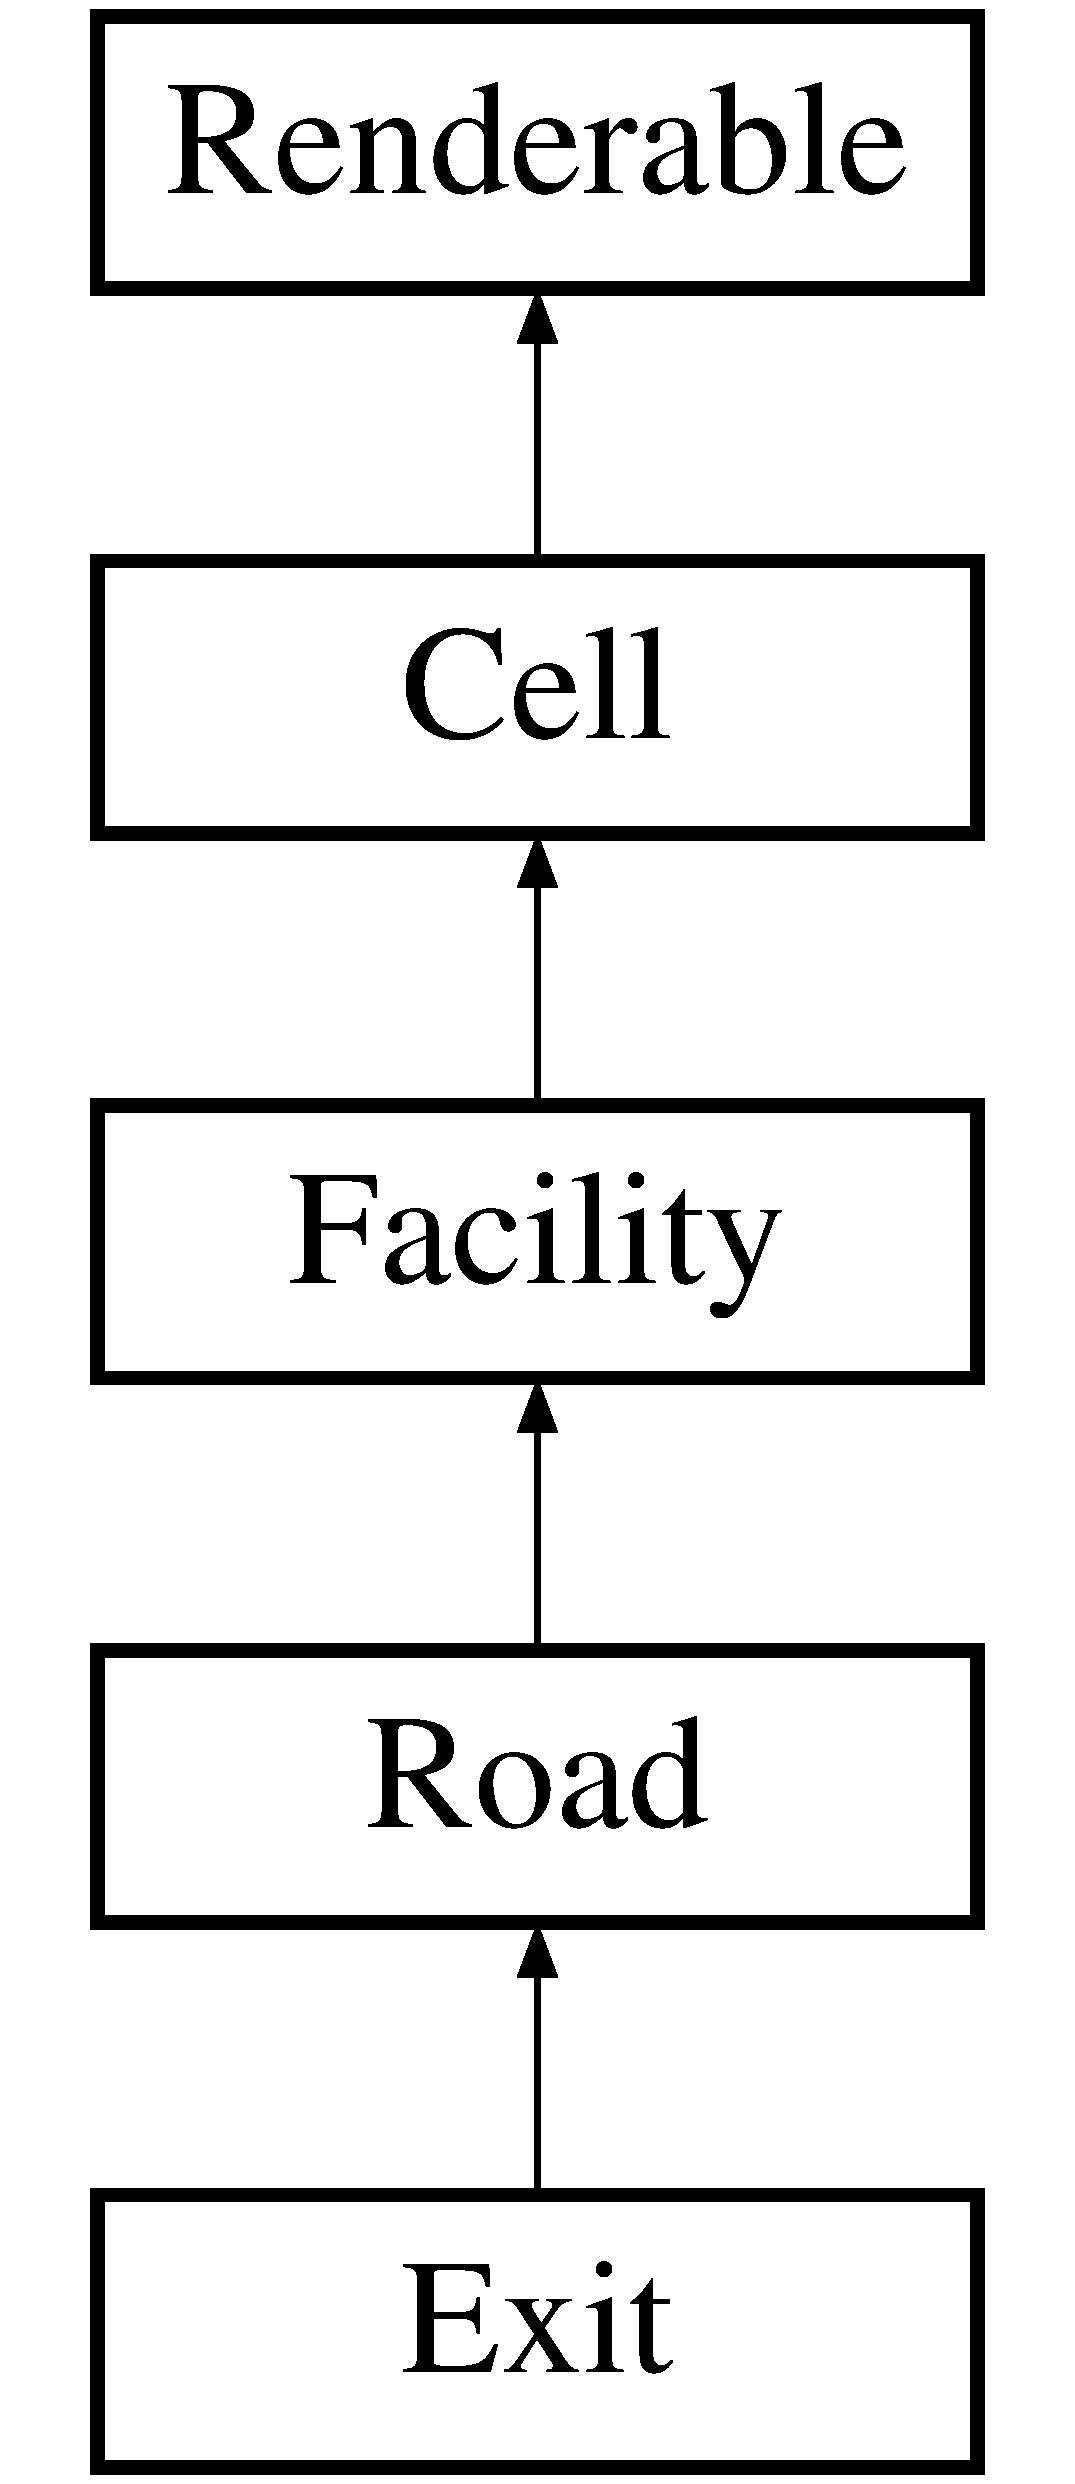
\includegraphics[height=5.000000cm]{classExit}
\end{center}
\end{figure}
\subsection*{Public Member Functions}
\begin{DoxyCompactItemize}
\item 
\hyperlink{classExit_aa2014f2c72ebf359cdc583274939f705}{Exit} (int x, int y, char z)
\begin{DoxyCompactList}\small\item\em Constructor. \end{DoxyCompactList}\item 
string \hyperlink{classExit_aa769d720f40b684da6ca21fc2515f910}{get\-Tipe} ()
\begin{DoxyCompactList}\small\item\em Mendapatkan tipe \hyperlink{classCell}{Cell}. \end{DoxyCompactList}\end{DoxyCompactItemize}


\subsection{Detailed Description}
Kelas \hyperlink{classExit}{Exit} adalah kelas turunan dari \hyperlink{classRoad}{Road} 

\subsection{Constructor \& Destructor Documentation}
\hypertarget{classExit_aa2014f2c72ebf359cdc583274939f705}{\index{Exit@{Exit}!Exit@{Exit}}
\index{Exit@{Exit}!Exit@{Exit}}
\subsubsection[{Exit}]{\setlength{\rightskip}{0pt plus 5cm}Exit\-::\-Exit (
\begin{DoxyParamCaption}
\item[{int}]{x, }
\item[{int}]{y, }
\item[{char}]{z}
\end{DoxyParamCaption}
)}}\label{classExit_aa2014f2c72ebf359cdc583274939f705}


Constructor. 


\begin{DoxyParams}{Parameters}
{\em x} & Indeks baris \\
\hline
{\em y} & Indeks kolom \\
\hline
{\em s} & Simbol \\
\hline
\end{DoxyParams}


\subsection{Member Function Documentation}
\hypertarget{classExit_aa769d720f40b684da6ca21fc2515f910}{\index{Exit@{Exit}!get\-Tipe@{get\-Tipe}}
\index{get\-Tipe@{get\-Tipe}!Exit@{Exit}}
\subsubsection[{get\-Tipe}]{\setlength{\rightskip}{0pt plus 5cm}string Exit\-::get\-Tipe (
\begin{DoxyParamCaption}
{}
\end{DoxyParamCaption}
)\hspace{0.3cm}{\ttfamily [virtual]}}}\label{classExit_aa769d720f40b684da6ca21fc2515f910}


Mendapatkan tipe \hyperlink{classCell}{Cell}. 

\begin{DoxyReturn}{Returns}
tipe 
\end{DoxyReturn}


Reimplemented from \hyperlink{classRoad_a750f8b4ab694ed29e8bd6db4d9758429}{Road}.



The documentation for this class was generated from the following files\-:\begin{DoxyCompactItemize}
\item 
Exit.\-h\item 
Exit.\-cpp\end{DoxyCompactItemize}

\hypertarget{classFacility}{\section{Facility Class Reference}
\label{classFacility}\index{Facility@{Facility}}
}


{\ttfamily \#include $<$Facility.\-h$>$}

Inheritance diagram for Facility\-:\begin{figure}[H]
\begin{center}
\leavevmode
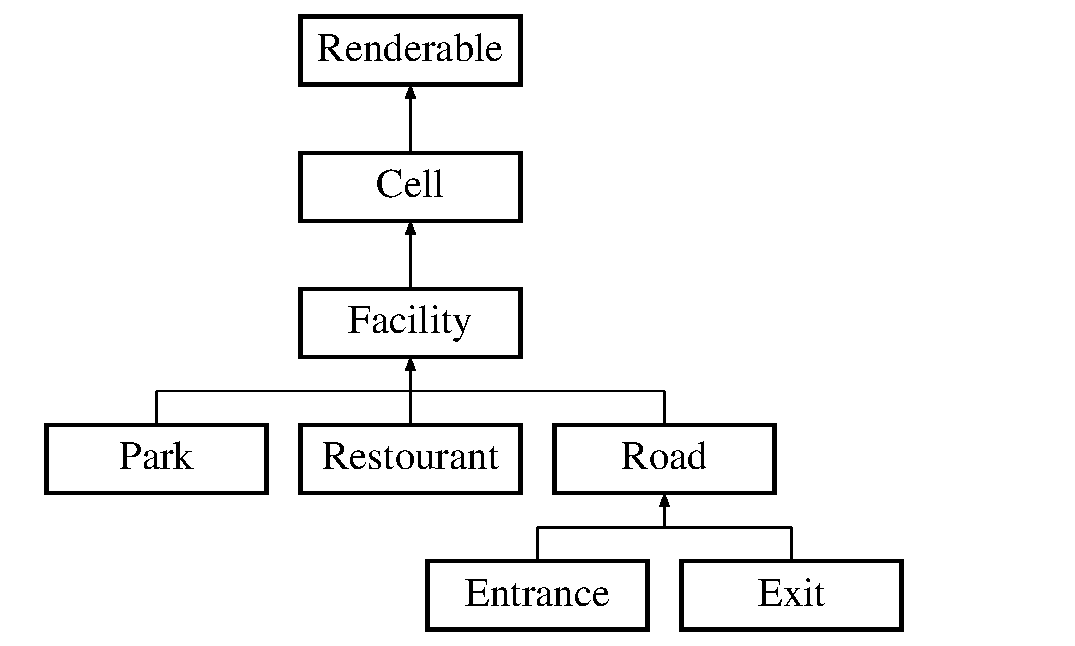
\includegraphics[height=5.000000cm]{classFacility}
\end{center}
\end{figure}
\subsection*{Public Member Functions}
\begin{DoxyCompactItemize}
\item 
\hyperlink{classFacility_a9b454613a038131abe556706405f4d74}{Facility} (int x, int y, char s)
\begin{DoxyCompactList}\small\item\em Constructor. \end{DoxyCompactList}\item 
virtual string \hyperlink{classFacility_a0350c1492460c160c95b1be72ea09860}{get\-Tipe} ()=0
\begin{DoxyCompactList}\small\item\em Mendapatkan tipe \hyperlink{classCell}{Cell}. \end{DoxyCompactList}\end{DoxyCompactItemize}


\subsection{Detailed Description}
Kelas \hyperlink{classFacility}{Facility} adalah kelas turunan dari \hyperlink{classCell}{Cell} 

\subsection{Constructor \& Destructor Documentation}
\hypertarget{classFacility_a9b454613a038131abe556706405f4d74}{\index{Facility@{Facility}!Facility@{Facility}}
\index{Facility@{Facility}!Facility@{Facility}}
\subsubsection[{Facility}]{\setlength{\rightskip}{0pt plus 5cm}Facility\-::\-Facility (
\begin{DoxyParamCaption}
\item[{int}]{x, }
\item[{int}]{y, }
\item[{char}]{s}
\end{DoxyParamCaption}
)}}\label{classFacility_a9b454613a038131abe556706405f4d74}


Constructor. 


\begin{DoxyParams}{Parameters}
{\em x} & Indeks baris \\
\hline
{\em y} & Indeks kolom \\
\hline
{\em s} & Simbol \\
\hline
\end{DoxyParams}


\subsection{Member Function Documentation}
\hypertarget{classFacility_a0350c1492460c160c95b1be72ea09860}{\index{Facility@{Facility}!get\-Tipe@{get\-Tipe}}
\index{get\-Tipe@{get\-Tipe}!Facility@{Facility}}
\subsubsection[{get\-Tipe}]{\setlength{\rightskip}{0pt plus 5cm}virtual string Facility\-::get\-Tipe (
\begin{DoxyParamCaption}
{}
\end{DoxyParamCaption}
)\hspace{0.3cm}{\ttfamily [pure virtual]}}}\label{classFacility_a0350c1492460c160c95b1be72ea09860}


Mendapatkan tipe \hyperlink{classCell}{Cell}. 

\begin{DoxyReturn}{Returns}
tipe 
\end{DoxyReturn}


Implements \hyperlink{classCell_acf75f66796e8746df81dec0f7700ebbc}{Cell}.



Implemented in \hyperlink{classEntrance_afff61031d269e47536b3bf4821ab0dda}{Entrance}, \hyperlink{classExit_aa769d720f40b684da6ca21fc2515f910}{Exit}, \hyperlink{classPark_a2b8533d7c9e2024ccc58c57f89f192f2}{Park}, \hyperlink{classRestourant_a5f4f9f7229416a7c339bc08c7a50a991}{Restourant}, and \hyperlink{classRoad_a750f8b4ab694ed29e8bd6db4d9758429}{Road}.



The documentation for this class was generated from the following files\-:\begin{DoxyCompactItemize}
\item 
Facility.\-h\item 
Facility.\-cpp\end{DoxyCompactItemize}

\hypertarget{classFileReader}{\section{File\-Reader Class Reference}
\label{classFileReader}\index{File\-Reader@{File\-Reader}}
}


{\ttfamily \#include $<$file\-\_\-reader.\-h$>$}

\subsection*{Public Member Functions}
\begin{DoxyCompactItemize}
\item 
\hyperlink{classFileReader_a241d583987200240c86d267b80ef3f0a}{File\-Reader} (string namafile)
\begin{DoxyCompactList}\small\item\em Constructor \hyperlink{classFileReader}{File\-Reader}. \end{DoxyCompactList}\item 
\hypertarget{classFileReader_a1382969e8f1468f3b04ad4b44ab39dee}{\hyperlink{classFileReader_a1382969e8f1468f3b04ad4b44ab39dee}{$\sim$\-File\-Reader} ()}\label{classFileReader_a1382969e8f1468f3b04ad4b44ab39dee}

\begin{DoxyCompactList}\small\item\em Destruktor. \end{DoxyCompactList}\item 
\hypertarget{classFileReader_ac4a834d4f54c0ef1ce9a992f510eea41}{void \hyperlink{classFileReader_ac4a834d4f54c0ef1ce9a992f510eea41}{Read} ()}\label{classFileReader_ac4a834d4f54c0ef1ce9a992f510eea41}

\begin{DoxyCompactList}\small\item\em Membaca seluruh file. \end{DoxyCompactList}\item 
\hypertarget{classFileReader_a7d5f714729c507013c9a15ff300b9c26}{int \hyperlink{classFileReader_a7d5f714729c507013c9a15ff300b9c26}{Get\-Sum\-Cage\-Area} ()}\label{classFileReader_a7d5f714729c507013c9a15ff300b9c26}

\begin{DoxyCompactList}\small\item\em Getter. Mendapatkan total nilai cage\-Area. \end{DoxyCompactList}\item 
int \hyperlink{classFileReader_a546d60999827827b4cdccc8f943b813a}{Get\-N\-Brs} ()
\begin{DoxyCompactList}\small\item\em Getter. Mendapatkan nilai baris area Zoo. \end{DoxyCompactList}\item 
int \hyperlink{classFileReader_a5ac9938fe0188936d018da3be5f50376}{Get\-N\-Kol} ()
\begin{DoxyCompactList}\small\item\em Getter. Mendapatkan nilai kolom area Zoo. \end{DoxyCompactList}\item 
int \hyperlink{classFileReader_a20720a0ebdbbdbf78cfdfd204f513378}{Get\-N\-Cell\-Type} ()
\begin{DoxyCompactList}\small\item\em Getter. Mendapatkan jumlah tipe \hyperlink{classCell}{Cell} yang ada. \end{DoxyCompactList}\item 
int \hyperlink{classFileReader_acf0f6592e2d70ae0c30ecfd31b9542d8}{Get\-N\-Cage} ()
\begin{DoxyCompactList}\small\item\em Getter. Mendapatkan jumlah \hyperlink{classCage}{Cage} yang akan dibuat. \end{DoxyCompactList}\item 
string \hyperlink{classFileReader_a682b3ed91b920ba7fc0f6bf02ee2b7cb}{Get\-Cell\-Type} (int i)
\begin{DoxyCompactList}\small\item\em Getter. Mendapatkan tipe \hyperlink{classCell}{Cell} ke i. \end{DoxyCompactList}\item 
char \hyperlink{classFileReader_a658827df1193174f59ea615aee98e56b}{Get\-Cell\-Simbol} (int i)
\begin{DoxyCompactList}\small\item\em Getter. Mendapatkan simbol \hyperlink{classCell}{Cell} ke i. \end{DoxyCompactList}\item 
char \hyperlink{classFileReader_a1158227a3ca70debdec0b5a6d19a33af}{Get\-Maps} (int i, int j)
\begin{DoxyCompactList}\small\item\em Getter. Mendapatkan simbol \hyperlink{classCell}{Cell} pada maps\mbox{[}i\mbox{]}\mbox{[}j\mbox{]}. \end{DoxyCompactList}\item 
string \hyperlink{classFileReader_ab554f5ac48f82074f2718734bb8bcd82}{Get\-Cage\-Type} (int i)
\begin{DoxyCompactList}\small\item\em Getter. Mendapatkan tipe \hyperlink{classCage}{Cage} ke i. \end{DoxyCompactList}\item 
char \hyperlink{classFileReader_a085e4b6522e3a234a96891a74710e774}{Get\-Cage\-Simbol} (int i)
\begin{DoxyCompactList}\small\item\em Getter. Mendapatkan simbol \hyperlink{classCage}{Cage} ke i. \end{DoxyCompactList}\item 
int \hyperlink{classFileReader_a0e021e7e89ab6a788573791c409ae63e}{Get\-N\-Cage\-Area} (int i)
\begin{DoxyCompactList}\small\item\em Getter. Mendapatkan area \hyperlink{classCage}{Cage} ke i. \end{DoxyCompactList}\item 
int \hyperlink{classFileReader_a28187c28f4713125f55a928cbd7a9ce5}{Get\-N\-Animal} (int i)
\begin{DoxyCompactList}\small\item\em Getter. Mendapatkan jumlah \hyperlink{classAnimal}{Animal} ke i. \end{DoxyCompactList}\item 
int \hyperlink{classFileReader_a6739708d4e85ef4c8b9436178518f287}{Get\-Pos\-X} (int i)
\begin{DoxyCompactList}\small\item\em Getter. Mendapatkan posisi X \hyperlink{classCell}{Cell} \hyperlink{classCage}{Cage} ke i. \end{DoxyCompactList}\item 
int \hyperlink{classFileReader_a76fdd51b22001d088f55d1722668b455}{Get\-Pos\-Y} (int i)
\begin{DoxyCompactList}\small\item\em Getter. Mendapatkan posisi Y \hyperlink{classCell}{Cell} \hyperlink{classCage}{Cage} ke i. \end{DoxyCompactList}\end{DoxyCompactItemize}


\subsection{Detailed Description}
Kelas \hyperlink{classFileReader}{File\-Reader} adalah kelas untuk membaca konfigurasi Zoo dari file teks 

\subsection{Constructor \& Destructor Documentation}
\hypertarget{classFileReader_a241d583987200240c86d267b80ef3f0a}{\index{File\-Reader@{File\-Reader}!File\-Reader@{File\-Reader}}
\index{File\-Reader@{File\-Reader}!FileReader@{File\-Reader}}
\subsubsection[{File\-Reader}]{\setlength{\rightskip}{0pt plus 5cm}File\-Reader\-::\-File\-Reader (
\begin{DoxyParamCaption}
\item[{string}]{namafile}
\end{DoxyParamCaption}
)}}\label{classFileReader_a241d583987200240c86d267b80ef3f0a}


Constructor \hyperlink{classFileReader}{File\-Reader}. 


\begin{DoxyParams}{Parameters}
{\em namafile} & Namafile yang akan dibaca \\
\hline
\end{DoxyParams}


\subsection{Member Function Documentation}
\hypertarget{classFileReader_a085e4b6522e3a234a96891a74710e774}{\index{File\-Reader@{File\-Reader}!Get\-Cage\-Simbol@{Get\-Cage\-Simbol}}
\index{Get\-Cage\-Simbol@{Get\-Cage\-Simbol}!FileReader@{File\-Reader}}
\subsubsection[{Get\-Cage\-Simbol}]{\setlength{\rightskip}{0pt plus 5cm}char File\-Reader\-::\-Get\-Cage\-Simbol (
\begin{DoxyParamCaption}
\item[{int}]{i}
\end{DoxyParamCaption}
)}}\label{classFileReader_a085e4b6522e3a234a96891a74710e774}


Getter. Mendapatkan simbol \hyperlink{classCage}{Cage} ke i. 


\begin{DoxyParams}{Parameters}
{\em i} & Index simbol \hyperlink{classCage}{Cage} yang akan dikembalikan \\
\hline
\end{DoxyParams}
\begin{DoxyReturn}{Returns}
list\-Cage\-Simbol\mbox{[}i\mbox{]} 
\end{DoxyReturn}
\hypertarget{classFileReader_ab554f5ac48f82074f2718734bb8bcd82}{\index{File\-Reader@{File\-Reader}!Get\-Cage\-Type@{Get\-Cage\-Type}}
\index{Get\-Cage\-Type@{Get\-Cage\-Type}!FileReader@{File\-Reader}}
\subsubsection[{Get\-Cage\-Type}]{\setlength{\rightskip}{0pt plus 5cm}string File\-Reader\-::\-Get\-Cage\-Type (
\begin{DoxyParamCaption}
\item[{int}]{i}
\end{DoxyParamCaption}
)}}\label{classFileReader_ab554f5ac48f82074f2718734bb8bcd82}


Getter. Mendapatkan tipe \hyperlink{classCage}{Cage} ke i. 


\begin{DoxyParams}{Parameters}
{\em i} & Index tipe \hyperlink{classCage}{Cage} yang akan dikembalikan \\
\hline
\end{DoxyParams}
\begin{DoxyReturn}{Returns}
list\-Cage\-Type\mbox{[}i\mbox{]} 
\end{DoxyReturn}
\hypertarget{classFileReader_a658827df1193174f59ea615aee98e56b}{\index{File\-Reader@{File\-Reader}!Get\-Cell\-Simbol@{Get\-Cell\-Simbol}}
\index{Get\-Cell\-Simbol@{Get\-Cell\-Simbol}!FileReader@{File\-Reader}}
\subsubsection[{Get\-Cell\-Simbol}]{\setlength{\rightskip}{0pt plus 5cm}char File\-Reader\-::\-Get\-Cell\-Simbol (
\begin{DoxyParamCaption}
\item[{int}]{i}
\end{DoxyParamCaption}
)}}\label{classFileReader_a658827df1193174f59ea615aee98e56b}


Getter. Mendapatkan simbol \hyperlink{classCell}{Cell} ke i. 


\begin{DoxyParams}{Parameters}
{\em i} & Index simbol \hyperlink{classCell}{Cell} yang akan dikembalikan \\
\hline
\end{DoxyParams}
\begin{DoxyReturn}{Returns}
list\-Cell\-Simbol\mbox{[}i\mbox{]} 
\end{DoxyReturn}
\hypertarget{classFileReader_a682b3ed91b920ba7fc0f6bf02ee2b7cb}{\index{File\-Reader@{File\-Reader}!Get\-Cell\-Type@{Get\-Cell\-Type}}
\index{Get\-Cell\-Type@{Get\-Cell\-Type}!FileReader@{File\-Reader}}
\subsubsection[{Get\-Cell\-Type}]{\setlength{\rightskip}{0pt plus 5cm}string File\-Reader\-::\-Get\-Cell\-Type (
\begin{DoxyParamCaption}
\item[{int}]{i}
\end{DoxyParamCaption}
)}}\label{classFileReader_a682b3ed91b920ba7fc0f6bf02ee2b7cb}


Getter. Mendapatkan tipe \hyperlink{classCell}{Cell} ke i. 


\begin{DoxyParams}{Parameters}
{\em i} & Index tipe \hyperlink{classCell}{Cell} yang akan dikembalikan \\
\hline
\end{DoxyParams}
\begin{DoxyReturn}{Returns}
list\-Cell\-Type\mbox{[}i\mbox{]} 
\end{DoxyReturn}
\hypertarget{classFileReader_a1158227a3ca70debdec0b5a6d19a33af}{\index{File\-Reader@{File\-Reader}!Get\-Maps@{Get\-Maps}}
\index{Get\-Maps@{Get\-Maps}!FileReader@{File\-Reader}}
\subsubsection[{Get\-Maps}]{\setlength{\rightskip}{0pt plus 5cm}char File\-Reader\-::\-Get\-Maps (
\begin{DoxyParamCaption}
\item[{int}]{i, }
\item[{int}]{j}
\end{DoxyParamCaption}
)}}\label{classFileReader_a1158227a3ca70debdec0b5a6d19a33af}


Getter. Mendapatkan simbol \hyperlink{classCell}{Cell} pada maps\mbox{[}i\mbox{]}\mbox{[}j\mbox{]}. 


\begin{DoxyParams}{Parameters}
{\em i} & Index baris maps \\
\hline
{\em j} & Indeks kolom maps \\
\hline
\end{DoxyParams}
\begin{DoxyReturn}{Returns}
maps\mbox{[}i\mbox{]}\mbox{[}j\mbox{]} 
\end{DoxyReturn}
\hypertarget{classFileReader_a28187c28f4713125f55a928cbd7a9ce5}{\index{File\-Reader@{File\-Reader}!Get\-N\-Animal@{Get\-N\-Animal}}
\index{Get\-N\-Animal@{Get\-N\-Animal}!FileReader@{File\-Reader}}
\subsubsection[{Get\-N\-Animal}]{\setlength{\rightskip}{0pt plus 5cm}int File\-Reader\-::\-Get\-N\-Animal (
\begin{DoxyParamCaption}
\item[{int}]{i}
\end{DoxyParamCaption}
)}}\label{classFileReader_a28187c28f4713125f55a928cbd7a9ce5}


Getter. Mendapatkan jumlah \hyperlink{classAnimal}{Animal} ke i. 


\begin{DoxyParams}{Parameters}
{\em i} & Index jumlah \hyperlink{classAnimal}{Animal} yang akan dikembalikan \\
\hline
\end{DoxyParams}
\begin{DoxyReturn}{Returns}
list\-N\-Animal\mbox{[}i\mbox{]} 
\end{DoxyReturn}
\hypertarget{classFileReader_a546d60999827827b4cdccc8f943b813a}{\index{File\-Reader@{File\-Reader}!Get\-N\-Brs@{Get\-N\-Brs}}
\index{Get\-N\-Brs@{Get\-N\-Brs}!FileReader@{File\-Reader}}
\subsubsection[{Get\-N\-Brs}]{\setlength{\rightskip}{0pt plus 5cm}int File\-Reader\-::\-Get\-N\-Brs (
\begin{DoxyParamCaption}
{}
\end{DoxyParamCaption}
)}}\label{classFileReader_a546d60999827827b4cdccc8f943b813a}


Getter. Mendapatkan nilai baris area Zoo. 

\begin{DoxyReturn}{Returns}
nbrs 
\end{DoxyReturn}
\hypertarget{classFileReader_acf0f6592e2d70ae0c30ecfd31b9542d8}{\index{File\-Reader@{File\-Reader}!Get\-N\-Cage@{Get\-N\-Cage}}
\index{Get\-N\-Cage@{Get\-N\-Cage}!FileReader@{File\-Reader}}
\subsubsection[{Get\-N\-Cage}]{\setlength{\rightskip}{0pt plus 5cm}int File\-Reader\-::\-Get\-N\-Cage (
\begin{DoxyParamCaption}
{}
\end{DoxyParamCaption}
)}}\label{classFileReader_acf0f6592e2d70ae0c30ecfd31b9542d8}


Getter. Mendapatkan jumlah \hyperlink{classCage}{Cage} yang akan dibuat. 

\begin{DoxyReturn}{Returns}
n\-Cage 
\end{DoxyReturn}
\hypertarget{classFileReader_a0e021e7e89ab6a788573791c409ae63e}{\index{File\-Reader@{File\-Reader}!Get\-N\-Cage\-Area@{Get\-N\-Cage\-Area}}
\index{Get\-N\-Cage\-Area@{Get\-N\-Cage\-Area}!FileReader@{File\-Reader}}
\subsubsection[{Get\-N\-Cage\-Area}]{\setlength{\rightskip}{0pt plus 5cm}int File\-Reader\-::\-Get\-N\-Cage\-Area (
\begin{DoxyParamCaption}
\item[{int}]{i}
\end{DoxyParamCaption}
)}}\label{classFileReader_a0e021e7e89ab6a788573791c409ae63e}


Getter. Mendapatkan area \hyperlink{classCage}{Cage} ke i. 


\begin{DoxyParams}{Parameters}
{\em i} & Index area \hyperlink{classCage}{Cage} yang akan dikembalikan \\
\hline
\end{DoxyParams}
\begin{DoxyReturn}{Returns}
list\-N\-Cage\-Area\mbox{[}i\mbox{]} 
\end{DoxyReturn}
\hypertarget{classFileReader_a20720a0ebdbbdbf78cfdfd204f513378}{\index{File\-Reader@{File\-Reader}!Get\-N\-Cell\-Type@{Get\-N\-Cell\-Type}}
\index{Get\-N\-Cell\-Type@{Get\-N\-Cell\-Type}!FileReader@{File\-Reader}}
\subsubsection[{Get\-N\-Cell\-Type}]{\setlength{\rightskip}{0pt plus 5cm}int File\-Reader\-::\-Get\-N\-Cell\-Type (
\begin{DoxyParamCaption}
{}
\end{DoxyParamCaption}
)}}\label{classFileReader_a20720a0ebdbbdbf78cfdfd204f513378}


Getter. Mendapatkan jumlah tipe \hyperlink{classCell}{Cell} yang ada. 

\begin{DoxyReturn}{Returns}
n\-Cell\-Type 
\end{DoxyReturn}
\hypertarget{classFileReader_a5ac9938fe0188936d018da3be5f50376}{\index{File\-Reader@{File\-Reader}!Get\-N\-Kol@{Get\-N\-Kol}}
\index{Get\-N\-Kol@{Get\-N\-Kol}!FileReader@{File\-Reader}}
\subsubsection[{Get\-N\-Kol}]{\setlength{\rightskip}{0pt plus 5cm}int File\-Reader\-::\-Get\-N\-Kol (
\begin{DoxyParamCaption}
{}
\end{DoxyParamCaption}
)}}\label{classFileReader_a5ac9938fe0188936d018da3be5f50376}


Getter. Mendapatkan nilai kolom area Zoo. 

\begin{DoxyReturn}{Returns}
nkol 
\end{DoxyReturn}
\hypertarget{classFileReader_a6739708d4e85ef4c8b9436178518f287}{\index{File\-Reader@{File\-Reader}!Get\-Pos\-X@{Get\-Pos\-X}}
\index{Get\-Pos\-X@{Get\-Pos\-X}!FileReader@{File\-Reader}}
\subsubsection[{Get\-Pos\-X}]{\setlength{\rightskip}{0pt plus 5cm}int File\-Reader\-::\-Get\-Pos\-X (
\begin{DoxyParamCaption}
\item[{int}]{i}
\end{DoxyParamCaption}
)}}\label{classFileReader_a6739708d4e85ef4c8b9436178518f287}


Getter. Mendapatkan posisi X \hyperlink{classCell}{Cell} \hyperlink{classCage}{Cage} ke i. 


\begin{DoxyParams}{Parameters}
{\em i} & Index posisi X \hyperlink{classCell}{Cell} \hyperlink{classCage}{Cage} yang akan dikembalikan \\
\hline
\end{DoxyParams}
\begin{DoxyReturn}{Returns}
list\-Pos\mbox{[}i\mbox{]}\mbox{[}0\mbox{]} 
\end{DoxyReturn}
\hypertarget{classFileReader_a76fdd51b22001d088f55d1722668b455}{\index{File\-Reader@{File\-Reader}!Get\-Pos\-Y@{Get\-Pos\-Y}}
\index{Get\-Pos\-Y@{Get\-Pos\-Y}!FileReader@{File\-Reader}}
\subsubsection[{Get\-Pos\-Y}]{\setlength{\rightskip}{0pt plus 5cm}int File\-Reader\-::\-Get\-Pos\-Y (
\begin{DoxyParamCaption}
\item[{int}]{i}
\end{DoxyParamCaption}
)}}\label{classFileReader_a76fdd51b22001d088f55d1722668b455}


Getter. Mendapatkan posisi Y \hyperlink{classCell}{Cell} \hyperlink{classCage}{Cage} ke i. 


\begin{DoxyParams}{Parameters}
{\em i} & Index posisi Y \hyperlink{classCell}{Cell} \hyperlink{classCage}{Cage} yang akan dikembalikan \\
\hline
\end{DoxyParams}
\begin{DoxyReturn}{Returns}
list\-Pos\mbox{[}i\mbox{]}\mbox{[}1\mbox{]} 
\end{DoxyReturn}


The documentation for this class was generated from the following files\-:\begin{DoxyCompactItemize}
\item 
file\-\_\-reader.\-h\item 
file\-\_\-reader.\-cpp\end{DoxyCompactItemize}

\hypertarget{classFish}{\section{Fish Class Reference}
\label{classFish}\index{Fish@{Fish}}
}


{\ttfamily \#include $<$Fish.\-h$>$}

Inheritance diagram for Fish\-:\begin{figure}[H]
\begin{center}
\leavevmode
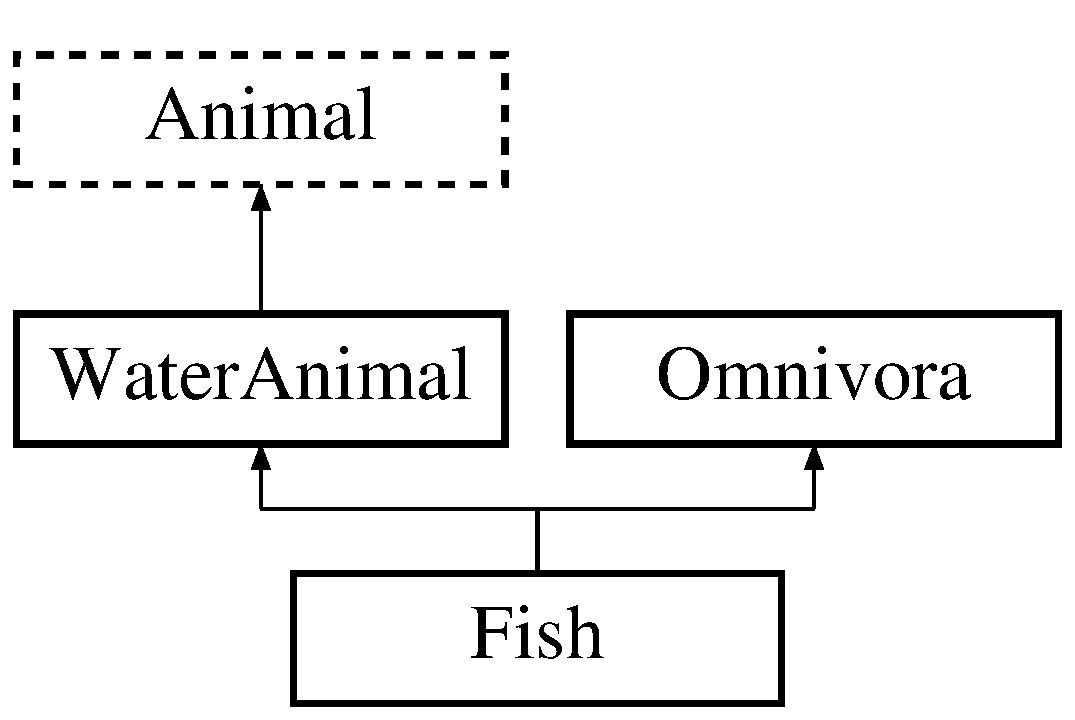
\includegraphics[height=3.000000cm]{classFish}
\end{center}
\end{figure}
\subsection*{Public Member Functions}
\begin{DoxyCompactItemize}
\item 
\hyperlink{classFish_ab1571c3fdf3033dbf21851b52f71288d}{Fish} (int \-\_\-x, int \-\_\-y)
\begin{DoxyCompactList}\small\item\em Constructor. \end{DoxyCompactList}\item 
\hypertarget{classFish_a23885c7956e22f0181360098cfe16659}{\hyperlink{classFish_a23885c7956e22f0181360098cfe16659}{$\sim$\-Fish} ()}\label{classFish_a23885c7956e22f0181360098cfe16659}

\begin{DoxyCompactList}\small\item\em Destructor. \end{DoxyCompactList}\item 
\hypertarget{classFish_acfab5585f69d7c1f786163530168ff11}{void \hyperlink{classFish_acfab5585f69d7c1f786163530168ff11}{add\-Bobot} ()}\label{classFish_acfab5585f69d7c1f786163530168ff11}

\begin{DoxyCompactList}\small\item\em Menambahkan bobot satu satuan. \end{DoxyCompactList}\item 
int \hyperlink{classFish_a3784ee11609ee4333d58468234a33c34}{get\-Bobot} ()
\begin{DoxyCompactList}\small\item\em Mendapatkan nilai bobot dari \hyperlink{classFish}{Fish}. \end{DoxyCompactList}\item 
char \hyperlink{classFish_adca0f30d1999f94c6c4bfce15a195f7f}{get\-Simbol} ()
\begin{DoxyCompactList}\small\item\em Mendapatkan simbol dari \hyperlink{classFish}{Fish}. \end{DoxyCompactList}\item 
string \hyperlink{classFish_ad576d177ba8b6ff98502d559e7584177}{get\-Musuh} (int i)
\begin{DoxyCompactList}\small\item\em Mendapatkan musuh ke i dari \hyperlink{classFish}{Fish} Musuh merupakan \hyperlink{classAnimal}{Animal} lain yang tidak bisa tinggal dalam satu kandang dengan \hyperlink{classFish}{Fish}. \end{DoxyCompactList}\item 
string \hyperlink{classFish_a15708e2598e6b5f20bf8b9b578db3eae}{interact} ()
\begin{DoxyCompactList}\small\item\em Mendapatkan reaksi \hyperlink{classFish}{Fish} saat berinteraksi dengan pengunjung. \end{DoxyCompactList}\item 
string \hyperlink{classFish_ac97e9f2a7652627b63f75cc0ef588578}{get\-Tipe\-Animal} ()
\begin{DoxyCompactList}\small\item\em Mendapatkan tipe \hyperlink{classAnimal}{Animal} (nama spesies) \end{DoxyCompactList}\end{DoxyCompactItemize}
\subsection*{Protected Attributes}
\begin{DoxyCompactItemize}
\item 
\hypertarget{classFish_a39c2658b3457b8b00239dbde823257a9}{const string {\bfseries tipe\-Animal} = \char`\"{}fish\char`\"{}}\label{classFish_a39c2658b3457b8b00239dbde823257a9}

\item 
\hypertarget{classFish_a97bdcd79503d461fc029c3f39971c349}{const char {\bfseries simbol} = 'i'}\label{classFish_a97bdcd79503d461fc029c3f39971c349}

\item 
\hypertarget{classFish_a59d3d28453939825a9cb71e384fb2044}{int {\bfseries bobot}}\label{classFish_a59d3d28453939825a9cb71e384fb2044}

\item 
\hypertarget{classFish_aacec01938a2e93d51b8d3a1fb093f921}{string $\ast$ {\bfseries musuh}}\label{classFish_aacec01938a2e93d51b8d3a1fb093f921}

\end{DoxyCompactItemize}


\subsection{Detailed Description}
Merupakan \hyperlink{classAnimal}{Animal} yang tinggal di air dan merupakan \hyperlink{classOmnivora}{Omnivora} 

\subsection{Constructor \& Destructor Documentation}
\hypertarget{classFish_ab1571c3fdf3033dbf21851b52f71288d}{\index{Fish@{Fish}!Fish@{Fish}}
\index{Fish@{Fish}!Fish@{Fish}}
\subsubsection[{Fish}]{\setlength{\rightskip}{0pt plus 5cm}Fish\-::\-Fish (
\begin{DoxyParamCaption}
\item[{int}]{\-\_\-x, }
\item[{int}]{\-\_\-y}
\end{DoxyParamCaption}
)}}\label{classFish_ab1571c3fdf3033dbf21851b52f71288d}


Constructor. 


\begin{DoxyParams}{Parameters}
{\em \-\_\-x} & posisi x awal \hyperlink{classFish}{Fish} \\
\hline
{\em \-\_\-y} & posisi y awal \hyperlink{classFish}{Fish} \\
\hline
\end{DoxyParams}


\subsection{Member Function Documentation}
\hypertarget{classFish_a3784ee11609ee4333d58468234a33c34}{\index{Fish@{Fish}!get\-Bobot@{get\-Bobot}}
\index{get\-Bobot@{get\-Bobot}!Fish@{Fish}}
\subsubsection[{get\-Bobot}]{\setlength{\rightskip}{0pt plus 5cm}int Fish\-::get\-Bobot (
\begin{DoxyParamCaption}
{}
\end{DoxyParamCaption}
)\hspace{0.3cm}{\ttfamily [virtual]}}}\label{classFish_a3784ee11609ee4333d58468234a33c34}


Mendapatkan nilai bobot dari \hyperlink{classFish}{Fish}. 

\begin{DoxyReturn}{Returns}
bobot 
\end{DoxyReturn}


Implements \hyperlink{classAnimal}{Animal}.

\hypertarget{classFish_ad576d177ba8b6ff98502d559e7584177}{\index{Fish@{Fish}!get\-Musuh@{get\-Musuh}}
\index{get\-Musuh@{get\-Musuh}!Fish@{Fish}}
\subsubsection[{get\-Musuh}]{\setlength{\rightskip}{0pt plus 5cm}string Fish\-::get\-Musuh (
\begin{DoxyParamCaption}
\item[{int}]{i}
\end{DoxyParamCaption}
)\hspace{0.3cm}{\ttfamily [virtual]}}}\label{classFish_ad576d177ba8b6ff98502d559e7584177}


Mendapatkan musuh ke i dari \hyperlink{classFish}{Fish} Musuh merupakan \hyperlink{classAnimal}{Animal} lain yang tidak bisa tinggal dalam satu kandang dengan \hyperlink{classFish}{Fish}. 

\begin{DoxyReturn}{Returns}
musuh\mbox{[}i\mbox{]} 
\end{DoxyReturn}


Implements \hyperlink{classAnimal}{Animal}.

\hypertarget{classFish_adca0f30d1999f94c6c4bfce15a195f7f}{\index{Fish@{Fish}!get\-Simbol@{get\-Simbol}}
\index{get\-Simbol@{get\-Simbol}!Fish@{Fish}}
\subsubsection[{get\-Simbol}]{\setlength{\rightskip}{0pt plus 5cm}char Fish\-::get\-Simbol (
\begin{DoxyParamCaption}
{}
\end{DoxyParamCaption}
)\hspace{0.3cm}{\ttfamily [virtual]}}}\label{classFish_adca0f30d1999f94c6c4bfce15a195f7f}


Mendapatkan simbol dari \hyperlink{classFish}{Fish}. 

\begin{DoxyReturn}{Returns}
simbol 
\end{DoxyReturn}


Implements \hyperlink{classAnimal}{Animal}.

\hypertarget{classFish_ac97e9f2a7652627b63f75cc0ef588578}{\index{Fish@{Fish}!get\-Tipe\-Animal@{get\-Tipe\-Animal}}
\index{get\-Tipe\-Animal@{get\-Tipe\-Animal}!Fish@{Fish}}
\subsubsection[{get\-Tipe\-Animal}]{\setlength{\rightskip}{0pt plus 5cm}string Fish\-::get\-Tipe\-Animal (
\begin{DoxyParamCaption}
{}
\end{DoxyParamCaption}
)\hspace{0.3cm}{\ttfamily [virtual]}}}\label{classFish_ac97e9f2a7652627b63f75cc0ef588578}


Mendapatkan tipe \hyperlink{classAnimal}{Animal} (nama spesies) 

\begin{DoxyReturn}{Returns}
tipe\-Animal 
\end{DoxyReturn}


Implements \hyperlink{classWaterAnimal}{Water\-Animal}.

\hypertarget{classFish_a15708e2598e6b5f20bf8b9b578db3eae}{\index{Fish@{Fish}!interact@{interact}}
\index{interact@{interact}!Fish@{Fish}}
\subsubsection[{interact}]{\setlength{\rightskip}{0pt plus 5cm}string Fish\-::interact (
\begin{DoxyParamCaption}
{}
\end{DoxyParamCaption}
)\hspace{0.3cm}{\ttfamily [virtual]}}}\label{classFish_a15708e2598e6b5f20bf8b9b578db3eae}


Mendapatkan reaksi \hyperlink{classFish}{Fish} saat berinteraksi dengan pengunjung. 

\begin{DoxyReturn}{Returns}
\char`\"{}wetwet\char`\"{} 
\end{DoxyReturn}


Implements \hyperlink{classWaterAnimal}{Water\-Animal}.



The documentation for this class was generated from the following files\-:\begin{DoxyCompactItemize}
\item 
Fish.\-h\item 
Fish.\-cpp\end{DoxyCompactItemize}

\hypertarget{classFlyingAnimal}{\section{Flying\-Animal Class Reference}
\label{classFlyingAnimal}\index{Flying\-Animal@{Flying\-Animal}}
}


{\ttfamily \#include $<$Flying\-Animal.\-h$>$}

Inheritance diagram for Flying\-Animal\-:\begin{figure}[H]
\begin{center}
\leavevmode
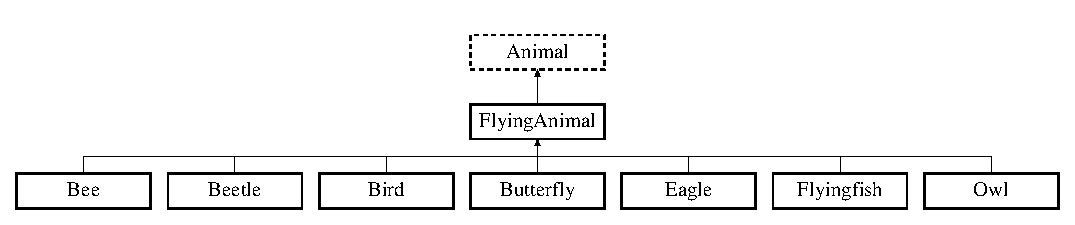
\includegraphics[height=2.580645cm]{classFlyingAnimal}
\end{center}
\end{figure}
\subsection*{Public Member Functions}
\begin{DoxyCompactItemize}
\item 
\hyperlink{classFlyingAnimal_abce03fb40df688bc103f6a9e5d185fd1}{Flying\-Animal} (int \-\_\-x, int \-\_\-y)
\begin{DoxyCompactList}\small\item\em Constructor. \end{DoxyCompactList}\item 
\hypertarget{classFlyingAnimal_ab2209a5b0286a65e2908a2fb7565e600}{\hyperlink{classFlyingAnimal_ab2209a5b0286a65e2908a2fb7565e600}{Flying\-Animal} (const \hyperlink{classFlyingAnimal}{Flying\-Animal} \&)}\label{classFlyingAnimal_ab2209a5b0286a65e2908a2fb7565e600}

\begin{DoxyCompactList}\small\item\em Copy Constructor. \end{DoxyCompactList}\item 
\hypertarget{classFlyingAnimal_a50a93cfcb6d0f216032279f463347544}{virtual \hyperlink{classFlyingAnimal_a50a93cfcb6d0f216032279f463347544}{$\sim$\-Flying\-Animal} ()}\label{classFlyingAnimal_a50a93cfcb6d0f216032279f463347544}

\begin{DoxyCompactList}\small\item\em Destructor. \end{DoxyCompactList}\item 
\hypertarget{classFlyingAnimal_ac0eee625fa2235eee8cbdc0a010ae430}{virtual string \hyperlink{classFlyingAnimal_ac0eee625fa2235eee8cbdc0a010ae430}{interact} ()=0}\label{classFlyingAnimal_ac0eee625fa2235eee8cbdc0a010ae430}

\begin{DoxyCompactList}\small\item\em Mendapatkan reaksi saat berinteraksi dengan pengunjung. \end{DoxyCompactList}\item 
virtual string \hyperlink{classFlyingAnimal_abc4d78229fe8a38ea786c519b4551e6e}{get\-Tipe\-Habitat} ()
\begin{DoxyCompactList}\small\item\em Mendapatkan tipe habitat. \end{DoxyCompactList}\item 
virtual string \hyperlink{classFlyingAnimal_a1523973b9a6a47e9064825c2134fd65d}{get\-Tipe\-Animal} ()=0
\begin{DoxyCompactList}\small\item\em Mendapatkan tipe \hyperlink{classAnimal}{Animal} (nama spesies) \end{DoxyCompactList}\end{DoxyCompactItemize}
\subsection*{Protected Attributes}
\begin{DoxyCompactItemize}
\item 
\hypertarget{classFlyingAnimal_a51653e2a708b6b85ee96fc2c4ee278c4}{const string {\bfseries tipe\-Habitat} = \char`\"{}air\char`\"{}}\label{classFlyingAnimal_a51653e2a708b6b85ee96fc2c4ee278c4}

\end{DoxyCompactItemize}


\subsection{Detailed Description}
Merupakan \hyperlink{classAnimal}{Animal} yang tinggal di udara 

\subsection{Constructor \& Destructor Documentation}
\hypertarget{classFlyingAnimal_abce03fb40df688bc103f6a9e5d185fd1}{\index{Flying\-Animal@{Flying\-Animal}!Flying\-Animal@{Flying\-Animal}}
\index{Flying\-Animal@{Flying\-Animal}!FlyingAnimal@{Flying\-Animal}}
\subsubsection[{Flying\-Animal}]{\setlength{\rightskip}{0pt plus 5cm}Flying\-Animal\-::\-Flying\-Animal (
\begin{DoxyParamCaption}
\item[{int}]{\-\_\-x, }
\item[{int}]{\-\_\-y}
\end{DoxyParamCaption}
)}}\label{classFlyingAnimal_abce03fb40df688bc103f6a9e5d185fd1}


Constructor. 


\begin{DoxyParams}{Parameters}
{\em \-\_\-x} & posisi x awal \hyperlink{classSnake}{Snake} \\
\hline
{\em \-\_\-y} & posisi y awal \hyperlink{classSnake}{Snake} \\
\hline
\end{DoxyParams}


\subsection{Member Function Documentation}
\hypertarget{classFlyingAnimal_a1523973b9a6a47e9064825c2134fd65d}{\index{Flying\-Animal@{Flying\-Animal}!get\-Tipe\-Animal@{get\-Tipe\-Animal}}
\index{get\-Tipe\-Animal@{get\-Tipe\-Animal}!FlyingAnimal@{Flying\-Animal}}
\subsubsection[{get\-Tipe\-Animal}]{\setlength{\rightskip}{0pt plus 5cm}virtual string Flying\-Animal\-::get\-Tipe\-Animal (
\begin{DoxyParamCaption}
{}
\end{DoxyParamCaption}
)\hspace{0.3cm}{\ttfamily [pure virtual]}}}\label{classFlyingAnimal_a1523973b9a6a47e9064825c2134fd65d}


Mendapatkan tipe \hyperlink{classAnimal}{Animal} (nama spesies) 

\begin{DoxyReturn}{Returns}
tipe\-Animal 
\end{DoxyReturn}


Implements \hyperlink{classAnimal}{Animal}.



Implemented in \hyperlink{classBird_a334d9a9e90114f5c74d2ad327120b2be}{Bird}, \hyperlink{classFlyingfish_a8e4bdebd6174a385ae894061b53b7cb1}{Flyingfish}, \hyperlink{classBee_a0341cf55086556e10104c7744f9fc833}{Bee}, \hyperlink{classBeetle_a30b538bbf1bf63ca615585bdc512ce33}{Beetle}, \hyperlink{classButterfly_a7a11185ad98c664b3d3f052336afec0e}{Butterfly}, \hyperlink{classEagle_af9d6c21fd2e046487b3490bb12ad3d6e}{Eagle}, and \hyperlink{classOwl_afbea38ace5450a7bde8caa813adbcfcd}{Owl}.

\hypertarget{classFlyingAnimal_abc4d78229fe8a38ea786c519b4551e6e}{\index{Flying\-Animal@{Flying\-Animal}!get\-Tipe\-Habitat@{get\-Tipe\-Habitat}}
\index{get\-Tipe\-Habitat@{get\-Tipe\-Habitat}!FlyingAnimal@{Flying\-Animal}}
\subsubsection[{get\-Tipe\-Habitat}]{\setlength{\rightskip}{0pt plus 5cm}string Flying\-Animal\-::get\-Tipe\-Habitat (
\begin{DoxyParamCaption}
{}
\end{DoxyParamCaption}
)\hspace{0.3cm}{\ttfamily [virtual]}}}\label{classFlyingAnimal_abc4d78229fe8a38ea786c519b4551e6e}


Mendapatkan tipe habitat. 

\begin{DoxyReturn}{Returns}
tipe\-Habitat 
\end{DoxyReturn}


Implements \hyperlink{classAnimal}{Animal}.



The documentation for this class was generated from the following files\-:\begin{DoxyCompactItemize}
\item 
Flying\-Animal.\-h\item 
Flying\-Animal.\-cpp\end{DoxyCompactItemize}

\hypertarget{classFlyingfish}{\section{Flyingfish Class Reference}
\label{classFlyingfish}\index{Flyingfish@{Flyingfish}}
}


{\ttfamily \#include $<$Flyingfish.\-h$>$}

Inheritance diagram for Flyingfish\-:\begin{figure}[H]
\begin{center}
\leavevmode
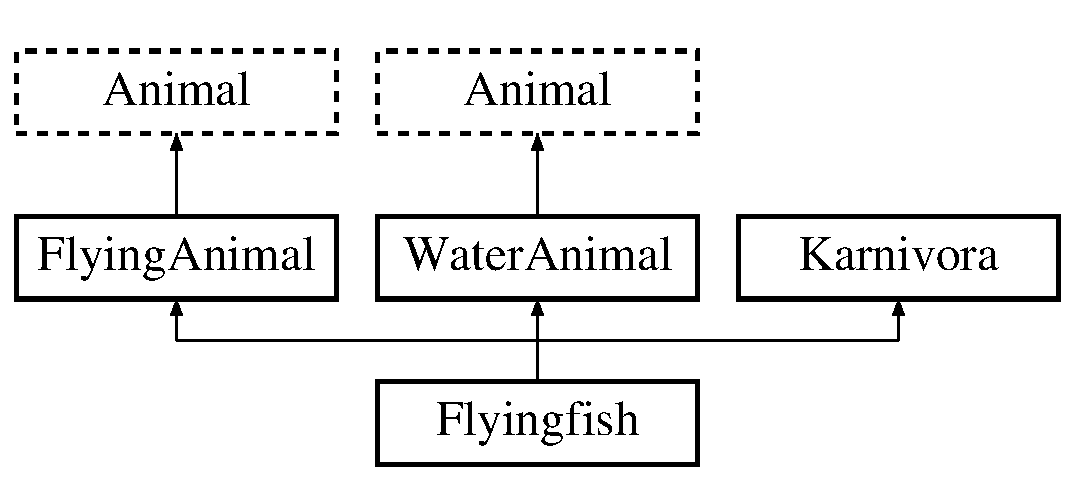
\includegraphics[height=3.000000cm]{classFlyingfish}
\end{center}
\end{figure}
\subsection*{Public Member Functions}
\begin{DoxyCompactItemize}
\item 
\hyperlink{classFlyingfish_a638286b5ea18b0db89c92c07553c05b3}{Flyingfish} (int \-\_\-x, int \-\_\-y)
\begin{DoxyCompactList}\small\item\em Constructor. \end{DoxyCompactList}\item 
\hypertarget{classFlyingfish_a8c3d3d1e4a09180306bb950dd71753c9}{\hyperlink{classFlyingfish_a8c3d3d1e4a09180306bb950dd71753c9}{$\sim$\-Flyingfish} ()}\label{classFlyingfish_a8c3d3d1e4a09180306bb950dd71753c9}

\begin{DoxyCompactList}\small\item\em Destructor. \end{DoxyCompactList}\item 
\hypertarget{classFlyingfish_a270d59756576de58bfedfde1607adbfe}{void \hyperlink{classFlyingfish_a270d59756576de58bfedfde1607adbfe}{add\-Bobot} ()}\label{classFlyingfish_a270d59756576de58bfedfde1607adbfe}

\begin{DoxyCompactList}\small\item\em Menambahkan bobot satu satuan. \end{DoxyCompactList}\item 
int \hyperlink{classFlyingfish_af2ece72f2ec7d09b45c47c7f20f8055f}{get\-Bobot} ()
\begin{DoxyCompactList}\small\item\em Mendapatkan nilai bobot dari \hyperlink{classFlyingfish}{Flyingfish}. \end{DoxyCompactList}\item 
char \hyperlink{classFlyingfish_ade9b5e0c9cbf6e129fef444828a39093}{get\-Simbol} ()
\begin{DoxyCompactList}\small\item\em Mendapatkan simbol dari \hyperlink{classFlyingfish}{Flyingfish}. \end{DoxyCompactList}\item 
string \hyperlink{classFlyingfish_a1b0c4e8ec03fed736df6bf8d21e6c5b4}{get\-Musuh} (int i)
\begin{DoxyCompactList}\small\item\em Mendapatkan musuh ke i dari \hyperlink{classFlyingfish}{Flyingfish} Musuh merupakan \hyperlink{classAnimal}{Animal} lain yang tidak bisa tinggal dalam satu kandang dengan \hyperlink{classFlyingfish}{Flyingfish}. \end{DoxyCompactList}\item 
string \hyperlink{classFlyingfish_a80a6975d988630970c7456c72c37591f}{interact} ()
\begin{DoxyCompactList}\small\item\em Mendapatkan reaksi \hyperlink{classFlyingfish}{Flyingfish} saat berinteraksi dengan pengunjung. \end{DoxyCompactList}\item 
string \hyperlink{classFlyingfish_a8e4bdebd6174a385ae894061b53b7cb1}{get\-Tipe\-Animal} ()
\begin{DoxyCompactList}\small\item\em Mendapatkan tipe \hyperlink{classAnimal}{Animal} (nama spesies) \end{DoxyCompactList}\end{DoxyCompactItemize}
\subsection*{Protected Attributes}
\begin{DoxyCompactItemize}
\item 
\hypertarget{classFlyingfish_a7e5623dfa2ef1d31681e88b9b987ca42}{const string {\bfseries tipe\-Animal} = \char`\"{}flyingfish\char`\"{}}\label{classFlyingfish_a7e5623dfa2ef1d31681e88b9b987ca42}

\item 
\hypertarget{classFlyingfish_ae1f06ca9e5a7df98d9f6efeec11b4fef}{const char {\bfseries simbol} = 'y'}\label{classFlyingfish_ae1f06ca9e5a7df98d9f6efeec11b4fef}

\item 
\hypertarget{classFlyingfish_abb0c372ce79f2aaf49fad4e3b99ff1fe}{int {\bfseries bobot}}\label{classFlyingfish_abb0c372ce79f2aaf49fad4e3b99ff1fe}

\item 
\hypertarget{classFlyingfish_a41d45887433cbbcab3f3787a3c24a093}{string $\ast$ {\bfseries musuh}}\label{classFlyingfish_a41d45887433cbbcab3f3787a3c24a093}

\end{DoxyCompactItemize}


\subsection{Detailed Description}
Merupakan \hyperlink{classAnimal}{Animal} yang tinggal di air dan udara dan merupakan \hyperlink{classKarnivora}{Karnivora} 

\subsection{Constructor \& Destructor Documentation}
\hypertarget{classFlyingfish_a638286b5ea18b0db89c92c07553c05b3}{\index{Flyingfish@{Flyingfish}!Flyingfish@{Flyingfish}}
\index{Flyingfish@{Flyingfish}!Flyingfish@{Flyingfish}}
\subsubsection[{Flyingfish}]{\setlength{\rightskip}{0pt plus 5cm}Flyingfish\-::\-Flyingfish (
\begin{DoxyParamCaption}
\item[{int}]{\-\_\-x, }
\item[{int}]{\-\_\-y}
\end{DoxyParamCaption}
)}}\label{classFlyingfish_a638286b5ea18b0db89c92c07553c05b3}


Constructor. 


\begin{DoxyParams}{Parameters}
{\em \-\_\-x} & posisi x awal \hyperlink{classFlyingfish}{Flyingfish} \\
\hline
{\em \-\_\-y} & posisi y awal \hyperlink{classFlyingfish}{Flyingfish} \\
\hline
\end{DoxyParams}


\subsection{Member Function Documentation}
\hypertarget{classFlyingfish_af2ece72f2ec7d09b45c47c7f20f8055f}{\index{Flyingfish@{Flyingfish}!get\-Bobot@{get\-Bobot}}
\index{get\-Bobot@{get\-Bobot}!Flyingfish@{Flyingfish}}
\subsubsection[{get\-Bobot}]{\setlength{\rightskip}{0pt plus 5cm}int Flyingfish\-::get\-Bobot (
\begin{DoxyParamCaption}
{}
\end{DoxyParamCaption}
)\hspace{0.3cm}{\ttfamily [virtual]}}}\label{classFlyingfish_af2ece72f2ec7d09b45c47c7f20f8055f}


Mendapatkan nilai bobot dari \hyperlink{classFlyingfish}{Flyingfish}. 

\begin{DoxyReturn}{Returns}
bobot 
\end{DoxyReturn}


Implements \hyperlink{classAnimal}{Animal}.

\hypertarget{classFlyingfish_a1b0c4e8ec03fed736df6bf8d21e6c5b4}{\index{Flyingfish@{Flyingfish}!get\-Musuh@{get\-Musuh}}
\index{get\-Musuh@{get\-Musuh}!Flyingfish@{Flyingfish}}
\subsubsection[{get\-Musuh}]{\setlength{\rightskip}{0pt plus 5cm}string Flyingfish\-::get\-Musuh (
\begin{DoxyParamCaption}
\item[{int}]{i}
\end{DoxyParamCaption}
)\hspace{0.3cm}{\ttfamily [virtual]}}}\label{classFlyingfish_a1b0c4e8ec03fed736df6bf8d21e6c5b4}


Mendapatkan musuh ke i dari \hyperlink{classFlyingfish}{Flyingfish} Musuh merupakan \hyperlink{classAnimal}{Animal} lain yang tidak bisa tinggal dalam satu kandang dengan \hyperlink{classFlyingfish}{Flyingfish}. 

\begin{DoxyReturn}{Returns}
musuh\mbox{[}i\mbox{]} 
\end{DoxyReturn}


Implements \hyperlink{classAnimal}{Animal}.

\hypertarget{classFlyingfish_ade9b5e0c9cbf6e129fef444828a39093}{\index{Flyingfish@{Flyingfish}!get\-Simbol@{get\-Simbol}}
\index{get\-Simbol@{get\-Simbol}!Flyingfish@{Flyingfish}}
\subsubsection[{get\-Simbol}]{\setlength{\rightskip}{0pt plus 5cm}char Flyingfish\-::get\-Simbol (
\begin{DoxyParamCaption}
{}
\end{DoxyParamCaption}
)\hspace{0.3cm}{\ttfamily [virtual]}}}\label{classFlyingfish_ade9b5e0c9cbf6e129fef444828a39093}


Mendapatkan simbol dari \hyperlink{classFlyingfish}{Flyingfish}. 

\begin{DoxyReturn}{Returns}
simbol 
\end{DoxyReturn}


Implements \hyperlink{classAnimal}{Animal}.

\hypertarget{classFlyingfish_a8e4bdebd6174a385ae894061b53b7cb1}{\index{Flyingfish@{Flyingfish}!get\-Tipe\-Animal@{get\-Tipe\-Animal}}
\index{get\-Tipe\-Animal@{get\-Tipe\-Animal}!Flyingfish@{Flyingfish}}
\subsubsection[{get\-Tipe\-Animal}]{\setlength{\rightskip}{0pt plus 5cm}string Flyingfish\-::get\-Tipe\-Animal (
\begin{DoxyParamCaption}
{}
\end{DoxyParamCaption}
)\hspace{0.3cm}{\ttfamily [virtual]}}}\label{classFlyingfish_a8e4bdebd6174a385ae894061b53b7cb1}


Mendapatkan tipe \hyperlink{classAnimal}{Animal} (nama spesies) 

\begin{DoxyReturn}{Returns}
tipe\-Animal 
\end{DoxyReturn}


Implements \hyperlink{classFlyingAnimal_a1523973b9a6a47e9064825c2134fd65d}{Flying\-Animal}.

\hypertarget{classFlyingfish_a80a6975d988630970c7456c72c37591f}{\index{Flyingfish@{Flyingfish}!interact@{interact}}
\index{interact@{interact}!Flyingfish@{Flyingfish}}
\subsubsection[{interact}]{\setlength{\rightskip}{0pt plus 5cm}string Flyingfish\-::interact (
\begin{DoxyParamCaption}
{}
\end{DoxyParamCaption}
)\hspace{0.3cm}{\ttfamily [virtual]}}}\label{classFlyingfish_a80a6975d988630970c7456c72c37591f}


Mendapatkan reaksi \hyperlink{classFlyingfish}{Flyingfish} saat berinteraksi dengan pengunjung. 

\begin{DoxyReturn}{Returns}
\char`\"{}flysplash\char`\"{} 
\end{DoxyReturn}


Implements \hyperlink{classFlyingAnimal_ac0eee625fa2235eee8cbdc0a010ae430}{Flying\-Animal}.



The documentation for this class was generated from the following files\-:\begin{DoxyCompactItemize}
\item 
Flyingfish.\-h\item 
Flyingfish.\-cpp\end{DoxyCompactItemize}

\hypertarget{classFrog}{\section{Frog Class Reference}
\label{classFrog}\index{Frog@{Frog}}
}


{\ttfamily \#include $<$Frog.\-h$>$}

Inheritance diagram for Frog\-:\begin{figure}[H]
\begin{center}
\leavevmode
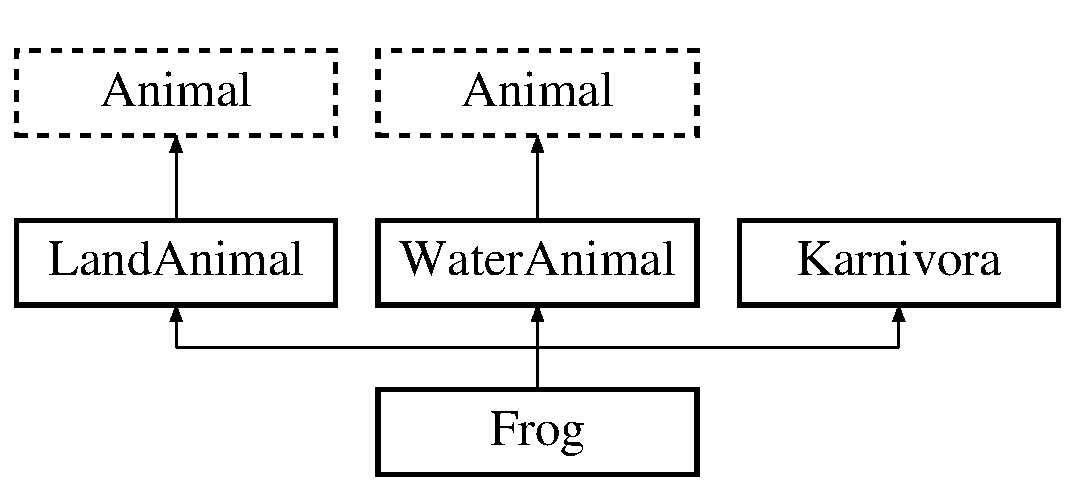
\includegraphics[height=3.000000cm]{classFrog}
\end{center}
\end{figure}
\subsection*{Public Member Functions}
\begin{DoxyCompactItemize}
\item 
\hyperlink{classFrog_a03e51490a1a0256508fb10031a8c9c4a}{Frog} (int \-\_\-x, int \-\_\-y)
\begin{DoxyCompactList}\small\item\em Constructor. \end{DoxyCompactList}\item 
\hypertarget{classFrog_a03c9cd2a028e2466a3bfe5e9af1c12e7}{\hyperlink{classFrog_a03c9cd2a028e2466a3bfe5e9af1c12e7}{$\sim$\-Frog} ()}\label{classFrog_a03c9cd2a028e2466a3bfe5e9af1c12e7}

\begin{DoxyCompactList}\small\item\em Destructor. \end{DoxyCompactList}\item 
\hypertarget{classFrog_adc65110eaafac9cf99e47b52f04a4050}{void \hyperlink{classFrog_adc65110eaafac9cf99e47b52f04a4050}{add\-Bobot} ()}\label{classFrog_adc65110eaafac9cf99e47b52f04a4050}

\begin{DoxyCompactList}\small\item\em Menambahkan bobot satu satuan. \end{DoxyCompactList}\item 
int \hyperlink{classFrog_af663e567deb96dc9ef3ff0a2a7f4b298}{get\-Bobot} ()
\begin{DoxyCompactList}\small\item\em Mendapatkan nilai bobot dari \hyperlink{classFrog}{Frog}. \end{DoxyCompactList}\item 
char \hyperlink{classFrog_a38e820c4f3510791ae7b8d40c9bd6b5a}{get\-Simbol} ()
\begin{DoxyCompactList}\small\item\em Mendapatkan simbol dari \hyperlink{classFrog}{Frog}. \end{DoxyCompactList}\item 
string \hyperlink{classFrog_a3968410026d8b2966b402ff5fdf87b59}{get\-Musuh} (int i)
\begin{DoxyCompactList}\small\item\em Mendapatkan musuh ke i dari \hyperlink{classFrog}{Frog} Musuh merupakan \hyperlink{classAnimal}{Animal} lain yang tidak bisa tinggal dalam satu kandang dengan \hyperlink{classFrog}{Frog}. \end{DoxyCompactList}\item 
string \hyperlink{classFrog_a7bf87b3cb6dfbee7b8de58a97796cadb}{interact} ()
\begin{DoxyCompactList}\small\item\em Mendapatkan reaksi \hyperlink{classFrog}{Frog} saat berinteraksi dengan pengunjung. \end{DoxyCompactList}\item 
string \hyperlink{classFrog_a9989ed2655d4f2bfeac06a82ef683f49}{get\-Tipe\-Animal} ()
\begin{DoxyCompactList}\small\item\em Mendapatkan tipe \hyperlink{classAnimal}{Animal} (nama spesies) \end{DoxyCompactList}\end{DoxyCompactItemize}
\subsection*{Protected Attributes}
\begin{DoxyCompactItemize}
\item 
\hypertarget{classFrog_a6add26d4bad17f506b263ca4b7ced01f}{const string {\bfseries tipe\-Animal} = \char`\"{}frog\char`\"{}}\label{classFrog_a6add26d4bad17f506b263ca4b7ced01f}

\item 
\hypertarget{classFrog_ac55b1dea99cd17daad20a801c26038b7}{const char {\bfseries simbol} = 'f'}\label{classFrog_ac55b1dea99cd17daad20a801c26038b7}

\item 
\hypertarget{classFrog_a442f9184b199d89f2b2f8208a8690688}{int {\bfseries bobot}}\label{classFrog_a442f9184b199d89f2b2f8208a8690688}

\item 
\hypertarget{classFrog_a621fcbd10e5b068689374e82b0e37359}{string $\ast$ {\bfseries musuh}}\label{classFrog_a621fcbd10e5b068689374e82b0e37359}

\end{DoxyCompactItemize}


\subsection{Detailed Description}
Merupakan \hyperlink{classAnimal}{Animal} yang tinggal di darat dan air dan merupakan \hyperlink{classKarnivora}{Karnivora} 

\subsection{Constructor \& Destructor Documentation}
\hypertarget{classFrog_a03e51490a1a0256508fb10031a8c9c4a}{\index{Frog@{Frog}!Frog@{Frog}}
\index{Frog@{Frog}!Frog@{Frog}}
\subsubsection[{Frog}]{\setlength{\rightskip}{0pt plus 5cm}Frog\-::\-Frog (
\begin{DoxyParamCaption}
\item[{int}]{\-\_\-x, }
\item[{int}]{\-\_\-y}
\end{DoxyParamCaption}
)}}\label{classFrog_a03e51490a1a0256508fb10031a8c9c4a}


Constructor. 


\begin{DoxyParams}{Parameters}
{\em \-\_\-x} & posisi x awal \hyperlink{classFrog}{Frog} \\
\hline
{\em \-\_\-y} & posisi y awal \hyperlink{classFrog}{Frog} \\
\hline
\end{DoxyParams}


\subsection{Member Function Documentation}
\hypertarget{classFrog_af663e567deb96dc9ef3ff0a2a7f4b298}{\index{Frog@{Frog}!get\-Bobot@{get\-Bobot}}
\index{get\-Bobot@{get\-Bobot}!Frog@{Frog}}
\subsubsection[{get\-Bobot}]{\setlength{\rightskip}{0pt plus 5cm}int Frog\-::get\-Bobot (
\begin{DoxyParamCaption}
{}
\end{DoxyParamCaption}
)\hspace{0.3cm}{\ttfamily [virtual]}}}\label{classFrog_af663e567deb96dc9ef3ff0a2a7f4b298}


Mendapatkan nilai bobot dari \hyperlink{classFrog}{Frog}. 

\begin{DoxyReturn}{Returns}
bobot 
\end{DoxyReturn}


Implements \hyperlink{classAnimal}{Animal}.

\hypertarget{classFrog_a3968410026d8b2966b402ff5fdf87b59}{\index{Frog@{Frog}!get\-Musuh@{get\-Musuh}}
\index{get\-Musuh@{get\-Musuh}!Frog@{Frog}}
\subsubsection[{get\-Musuh}]{\setlength{\rightskip}{0pt plus 5cm}string Frog\-::get\-Musuh (
\begin{DoxyParamCaption}
\item[{int}]{i}
\end{DoxyParamCaption}
)\hspace{0.3cm}{\ttfamily [virtual]}}}\label{classFrog_a3968410026d8b2966b402ff5fdf87b59}


Mendapatkan musuh ke i dari \hyperlink{classFrog}{Frog} Musuh merupakan \hyperlink{classAnimal}{Animal} lain yang tidak bisa tinggal dalam satu kandang dengan \hyperlink{classFrog}{Frog}. 

\begin{DoxyReturn}{Returns}
musuh\mbox{[}i\mbox{]} 
\end{DoxyReturn}


Implements \hyperlink{classAnimal}{Animal}.

\hypertarget{classFrog_a38e820c4f3510791ae7b8d40c9bd6b5a}{\index{Frog@{Frog}!get\-Simbol@{get\-Simbol}}
\index{get\-Simbol@{get\-Simbol}!Frog@{Frog}}
\subsubsection[{get\-Simbol}]{\setlength{\rightskip}{0pt plus 5cm}char Frog\-::get\-Simbol (
\begin{DoxyParamCaption}
{}
\end{DoxyParamCaption}
)\hspace{0.3cm}{\ttfamily [virtual]}}}\label{classFrog_a38e820c4f3510791ae7b8d40c9bd6b5a}


Mendapatkan simbol dari \hyperlink{classFrog}{Frog}. 

\begin{DoxyReturn}{Returns}
simbol 
\end{DoxyReturn}


Implements \hyperlink{classAnimal}{Animal}.

\hypertarget{classFrog_a9989ed2655d4f2bfeac06a82ef683f49}{\index{Frog@{Frog}!get\-Tipe\-Animal@{get\-Tipe\-Animal}}
\index{get\-Tipe\-Animal@{get\-Tipe\-Animal}!Frog@{Frog}}
\subsubsection[{get\-Tipe\-Animal}]{\setlength{\rightskip}{0pt plus 5cm}string Frog\-::get\-Tipe\-Animal (
\begin{DoxyParamCaption}
{}
\end{DoxyParamCaption}
)\hspace{0.3cm}{\ttfamily [virtual]}}}\label{classFrog_a9989ed2655d4f2bfeac06a82ef683f49}


Mendapatkan tipe \hyperlink{classAnimal}{Animal} (nama spesies) 

\begin{DoxyReturn}{Returns}
tipe\-Animal 
\end{DoxyReturn}


Implements \hyperlink{classLandAnimal}{Land\-Animal}.

\hypertarget{classFrog_a7bf87b3cb6dfbee7b8de58a97796cadb}{\index{Frog@{Frog}!interact@{interact}}
\index{interact@{interact}!Frog@{Frog}}
\subsubsection[{interact}]{\setlength{\rightskip}{0pt plus 5cm}string Frog\-::interact (
\begin{DoxyParamCaption}
{}
\end{DoxyParamCaption}
)\hspace{0.3cm}{\ttfamily [virtual]}}}\label{classFrog_a7bf87b3cb6dfbee7b8de58a97796cadb}


Mendapatkan reaksi \hyperlink{classFrog}{Frog} saat berinteraksi dengan pengunjung. 

\begin{DoxyReturn}{Returns}
\char`\"{}ribbit\char`\"{} 
\end{DoxyReturn}


Implements \hyperlink{classLandAnimal}{Land\-Animal}.



The documentation for this class was generated from the following files\-:\begin{DoxyCompactItemize}
\item 
Frog.\-h\item 
Frog.\-cpp\end{DoxyCompactItemize}

\hypertarget{classGoat}{\section{Goat Class Reference}
\label{classGoat}\index{Goat@{Goat}}
}


{\ttfamily \#include $<$Goat.\-h$>$}

Inheritance diagram for Goat\-:\begin{figure}[H]
\begin{center}
\leavevmode
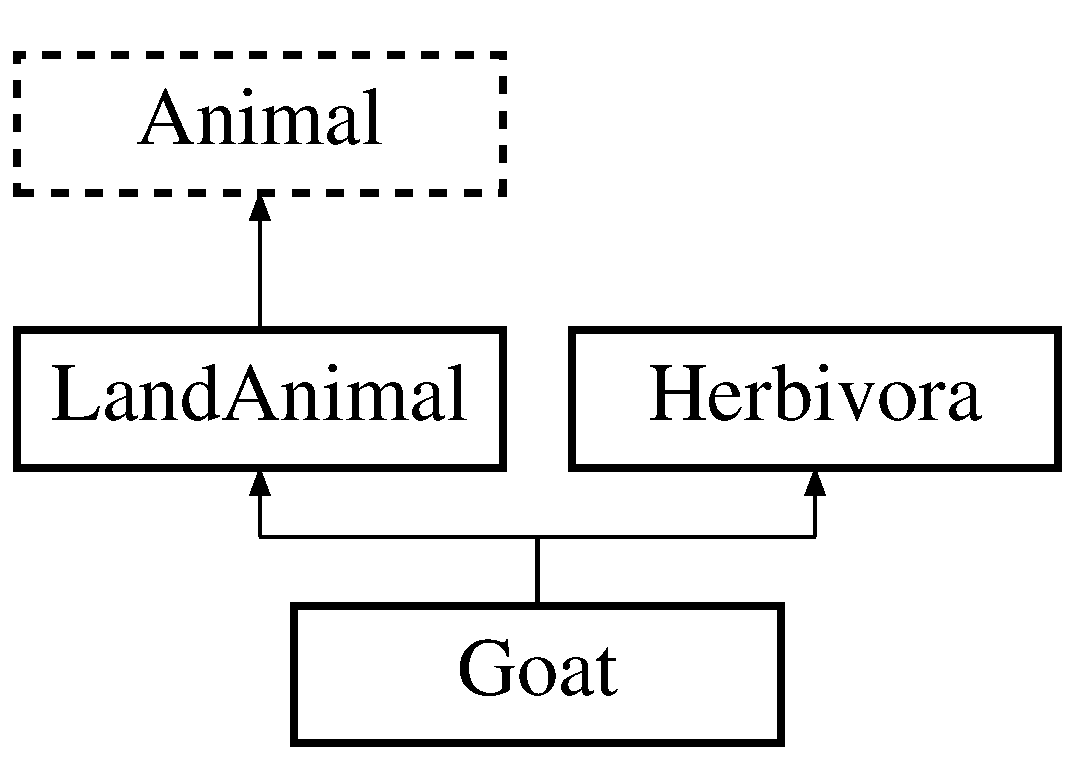
\includegraphics[height=3.000000cm]{classGoat}
\end{center}
\end{figure}
\subsection*{Public Member Functions}
\begin{DoxyCompactItemize}
\item 
\hyperlink{classGoat_a31a4d452fe7142fbc5fb2c7799a1a5d7}{Goat} (int \-\_\-x, int \-\_\-y)
\begin{DoxyCompactList}\small\item\em Constructor. \end{DoxyCompactList}\item 
\hypertarget{classGoat_aef1721f83327b7e46da9ad26173b42f8}{\hyperlink{classGoat_aef1721f83327b7e46da9ad26173b42f8}{$\sim$\-Goat} ()}\label{classGoat_aef1721f83327b7e46da9ad26173b42f8}

\begin{DoxyCompactList}\small\item\em Destructor. \end{DoxyCompactList}\item 
\hypertarget{classGoat_aacc8a4aeec7323e627c5ce6d5433973a}{void \hyperlink{classGoat_aacc8a4aeec7323e627c5ce6d5433973a}{add\-Bobot} ()}\label{classGoat_aacc8a4aeec7323e627c5ce6d5433973a}

\begin{DoxyCompactList}\small\item\em Menambahkan bobot satu satuan. \end{DoxyCompactList}\item 
int \hyperlink{classGoat_a0f5c5cce66f3447337754817ac079955}{get\-Bobot} ()
\begin{DoxyCompactList}\small\item\em Mendapatkan nilai bobot dari \hyperlink{classGoat}{Goat}. \end{DoxyCompactList}\item 
char \hyperlink{classGoat_a9de58c004a28fdd00f118edb560636b1}{get\-Simbol} ()
\begin{DoxyCompactList}\small\item\em Mendapatkan simbol dari \hyperlink{classGoat}{Goat}. \end{DoxyCompactList}\item 
string \hyperlink{classGoat_a789f9f47ef0646fe39c28df41bda8be5}{get\-Musuh} (int i)
\begin{DoxyCompactList}\small\item\em Mendapatkan musuh ke i dari \hyperlink{classGoat}{Goat} Musuh merupakan \hyperlink{classAnimal}{Animal} lain yang tidak bisa tinggal dalam satu kandang dengan \hyperlink{classGoat}{Goat}. \end{DoxyCompactList}\item 
string \hyperlink{classGoat_ac282f442721e8b8bb750eacd45df61b6}{interact} ()
\begin{DoxyCompactList}\small\item\em Mendapatkan reaksi \hyperlink{classGoat}{Goat} saat berinteraksi dengan pengunjung. \end{DoxyCompactList}\item 
string \hyperlink{classGoat_aca420bb0962e0b55339c8f70c217132b}{get\-Tipe\-Animal} ()
\begin{DoxyCompactList}\small\item\em Mendapatkan tipe \hyperlink{classAnimal}{Animal} (nama spesies) \end{DoxyCompactList}\end{DoxyCompactItemize}
\subsection*{Protected Attributes}
\begin{DoxyCompactItemize}
\item 
\hypertarget{classGoat_a0391d9cab6526907cd5d1074e8b87cc9}{const string {\bfseries tipe\-Animal} = \char`\"{}goat\char`\"{}}\label{classGoat_a0391d9cab6526907cd5d1074e8b87cc9}

\item 
\hypertarget{classGoat_a15a5f692bbaa8a22ba810f8c109937f2}{const char {\bfseries simbol} = 'g'}\label{classGoat_a15a5f692bbaa8a22ba810f8c109937f2}

\item 
\hypertarget{classGoat_a776c42e40f2b496d798e9bc302f99153}{int {\bfseries bobot}}\label{classGoat_a776c42e40f2b496d798e9bc302f99153}

\item 
\hypertarget{classGoat_a2ce75f8aa08563e9a5b7b05b4e4e6555}{string $\ast$ {\bfseries musuh}}\label{classGoat_a2ce75f8aa08563e9a5b7b05b4e4e6555}

\end{DoxyCompactItemize}


\subsection{Detailed Description}
Merupakan \hyperlink{classAnimal}{Animal} yang tinggal di darat dan merupakan \hyperlink{classKarnivora}{Karnivora} 

\subsection{Constructor \& Destructor Documentation}
\hypertarget{classGoat_a31a4d452fe7142fbc5fb2c7799a1a5d7}{\index{Goat@{Goat}!Goat@{Goat}}
\index{Goat@{Goat}!Goat@{Goat}}
\subsubsection[{Goat}]{\setlength{\rightskip}{0pt plus 5cm}Goat\-::\-Goat (
\begin{DoxyParamCaption}
\item[{int}]{\-\_\-x, }
\item[{int}]{\-\_\-y}
\end{DoxyParamCaption}
)}}\label{classGoat_a31a4d452fe7142fbc5fb2c7799a1a5d7}


Constructor. 


\begin{DoxyParams}{Parameters}
{\em \-\_\-x} & posisi x awal \hyperlink{classGoat}{Goat} \\
\hline
{\em \-\_\-y} & posisi y awal \hyperlink{classGoat}{Goat} \\
\hline
\end{DoxyParams}


\subsection{Member Function Documentation}
\hypertarget{classGoat_a0f5c5cce66f3447337754817ac079955}{\index{Goat@{Goat}!get\-Bobot@{get\-Bobot}}
\index{get\-Bobot@{get\-Bobot}!Goat@{Goat}}
\subsubsection[{get\-Bobot}]{\setlength{\rightskip}{0pt plus 5cm}int Goat\-::get\-Bobot (
\begin{DoxyParamCaption}
{}
\end{DoxyParamCaption}
)\hspace{0.3cm}{\ttfamily [virtual]}}}\label{classGoat_a0f5c5cce66f3447337754817ac079955}


Mendapatkan nilai bobot dari \hyperlink{classGoat}{Goat}. 

\begin{DoxyReturn}{Returns}
bobot 
\end{DoxyReturn}


Implements \hyperlink{classAnimal}{Animal}.

\hypertarget{classGoat_a789f9f47ef0646fe39c28df41bda8be5}{\index{Goat@{Goat}!get\-Musuh@{get\-Musuh}}
\index{get\-Musuh@{get\-Musuh}!Goat@{Goat}}
\subsubsection[{get\-Musuh}]{\setlength{\rightskip}{0pt plus 5cm}string Goat\-::get\-Musuh (
\begin{DoxyParamCaption}
\item[{int}]{i}
\end{DoxyParamCaption}
)\hspace{0.3cm}{\ttfamily [virtual]}}}\label{classGoat_a789f9f47ef0646fe39c28df41bda8be5}


Mendapatkan musuh ke i dari \hyperlink{classGoat}{Goat} Musuh merupakan \hyperlink{classAnimal}{Animal} lain yang tidak bisa tinggal dalam satu kandang dengan \hyperlink{classGoat}{Goat}. 

\begin{DoxyReturn}{Returns}
musuh\mbox{[}i\mbox{]} 
\end{DoxyReturn}


Implements \hyperlink{classAnimal}{Animal}.

\hypertarget{classGoat_a9de58c004a28fdd00f118edb560636b1}{\index{Goat@{Goat}!get\-Simbol@{get\-Simbol}}
\index{get\-Simbol@{get\-Simbol}!Goat@{Goat}}
\subsubsection[{get\-Simbol}]{\setlength{\rightskip}{0pt plus 5cm}char Goat\-::get\-Simbol (
\begin{DoxyParamCaption}
{}
\end{DoxyParamCaption}
)\hspace{0.3cm}{\ttfamily [virtual]}}}\label{classGoat_a9de58c004a28fdd00f118edb560636b1}


Mendapatkan simbol dari \hyperlink{classGoat}{Goat}. 

\begin{DoxyReturn}{Returns}
simbol 
\end{DoxyReturn}


Implements \hyperlink{classAnimal}{Animal}.

\hypertarget{classGoat_aca420bb0962e0b55339c8f70c217132b}{\index{Goat@{Goat}!get\-Tipe\-Animal@{get\-Tipe\-Animal}}
\index{get\-Tipe\-Animal@{get\-Tipe\-Animal}!Goat@{Goat}}
\subsubsection[{get\-Tipe\-Animal}]{\setlength{\rightskip}{0pt plus 5cm}string Goat\-::get\-Tipe\-Animal (
\begin{DoxyParamCaption}
{}
\end{DoxyParamCaption}
)\hspace{0.3cm}{\ttfamily [virtual]}}}\label{classGoat_aca420bb0962e0b55339c8f70c217132b}


Mendapatkan tipe \hyperlink{classAnimal}{Animal} (nama spesies) 

\begin{DoxyReturn}{Returns}
tipe\-Animal 
\end{DoxyReturn}


Implements \hyperlink{classLandAnimal}{Land\-Animal}.

\hypertarget{classGoat_ac282f442721e8b8bb750eacd45df61b6}{\index{Goat@{Goat}!interact@{interact}}
\index{interact@{interact}!Goat@{Goat}}
\subsubsection[{interact}]{\setlength{\rightskip}{0pt plus 5cm}string Goat\-::interact (
\begin{DoxyParamCaption}
{}
\end{DoxyParamCaption}
)\hspace{0.3cm}{\ttfamily [virtual]}}}\label{classGoat_ac282f442721e8b8bb750eacd45df61b6}


Mendapatkan reaksi \hyperlink{classGoat}{Goat} saat berinteraksi dengan pengunjung. 

\begin{DoxyReturn}{Returns}
\char`\"{}embeee\char`\"{} 
\end{DoxyReturn}


Implements \hyperlink{classLandAnimal}{Land\-Animal}.



The documentation for this class was generated from the following files\-:\begin{DoxyCompactItemize}
\item 
Goat.\-h\item 
Goat.\-cpp\end{DoxyCompactItemize}

\hypertarget{classHabitat}{\section{Habitat Class Reference}
\label{classHabitat}\index{Habitat@{Habitat}}
}


{\ttfamily \#include $<$Habitat.\-h$>$}

Inheritance diagram for Habitat\-:\begin{figure}[H]
\begin{center}
\leavevmode
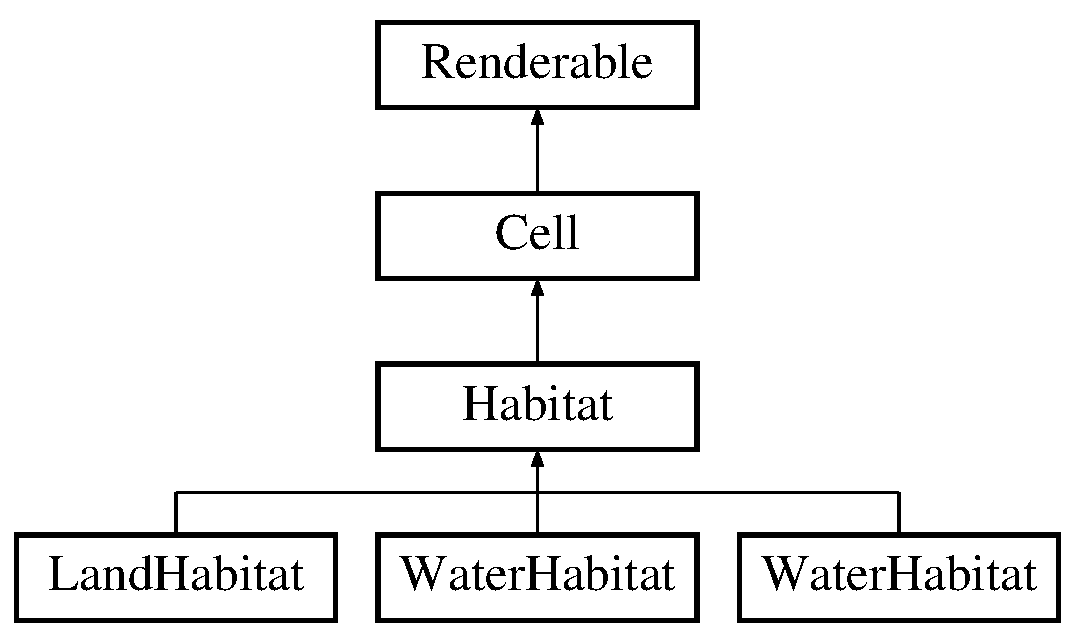
\includegraphics[height=4.000000cm]{classHabitat}
\end{center}
\end{figure}
\subsection*{Public Member Functions}
\begin{DoxyCompactItemize}
\item 
\hyperlink{classHabitat_a634a211938a290475733fe8463104fa0}{Habitat} (int x, int y, char z)
\begin{DoxyCompactList}\small\item\em Constructor. \end{DoxyCompactList}\item 
virtual string \hyperlink{classHabitat_a4c8164f06a0a32ca6c7f465380b31ac0}{get\-Tipe} ()=0
\begin{DoxyCompactList}\small\item\em Mendapatkan tipe \hyperlink{classCell}{Cell}. \end{DoxyCompactList}\end{DoxyCompactItemize}


\subsection{Detailed Description}
Kelas \hyperlink{classHabitat}{Habitat} adalah kelas turunan dari \hyperlink{classCell}{Cell} 

\subsection{Constructor \& Destructor Documentation}
\hypertarget{classHabitat_a634a211938a290475733fe8463104fa0}{\index{Habitat@{Habitat}!Habitat@{Habitat}}
\index{Habitat@{Habitat}!Habitat@{Habitat}}
\subsubsection[{Habitat}]{\setlength{\rightskip}{0pt plus 5cm}Habitat\-::\-Habitat (
\begin{DoxyParamCaption}
\item[{int}]{x, }
\item[{int}]{y, }
\item[{char}]{z}
\end{DoxyParamCaption}
)}}\label{classHabitat_a634a211938a290475733fe8463104fa0}


Constructor. 


\begin{DoxyParams}{Parameters}
{\em x} & Indeks baris \\
\hline
{\em y} & Indeks kolom \\
\hline
{\em s} & Simbol \\
\hline
\end{DoxyParams}


\subsection{Member Function Documentation}
\hypertarget{classHabitat_a4c8164f06a0a32ca6c7f465380b31ac0}{\index{Habitat@{Habitat}!get\-Tipe@{get\-Tipe}}
\index{get\-Tipe@{get\-Tipe}!Habitat@{Habitat}}
\subsubsection[{get\-Tipe}]{\setlength{\rightskip}{0pt plus 5cm}virtual string Habitat\-::get\-Tipe (
\begin{DoxyParamCaption}
{}
\end{DoxyParamCaption}
)\hspace{0.3cm}{\ttfamily [pure virtual]}}}\label{classHabitat_a4c8164f06a0a32ca6c7f465380b31ac0}


Mendapatkan tipe \hyperlink{classCell}{Cell}. 

\begin{DoxyReturn}{Returns}
tipe 
\end{DoxyReturn}


Implements \hyperlink{classCell_acf75f66796e8746df81dec0f7700ebbc}{Cell}.



Implemented in \hyperlink{classWaterHabitat_a02b4e524ab689f2e2b54b74acb58f7b2}{Water\-Habitat}, \hyperlink{classLandHabitat_a51ad769f1682ec5b45bcd8839e854575}{Land\-Habitat}, and \hyperlink{classWaterHabitat_a02b4e524ab689f2e2b54b74acb58f7b2}{Water\-Habitat}.



The documentation for this class was generated from the following files\-:\begin{DoxyCompactItemize}
\item 
Habitat.\-h\item 
Habitat.\-cpp\end{DoxyCompactItemize}

\hypertarget{classHedgehog}{\section{Hedgehog Class Reference}
\label{classHedgehog}\index{Hedgehog@{Hedgehog}}
}


{\ttfamily \#include $<$Hedgehog.\-h$>$}

Inheritance diagram for Hedgehog\-:\begin{figure}[H]
\begin{center}
\leavevmode
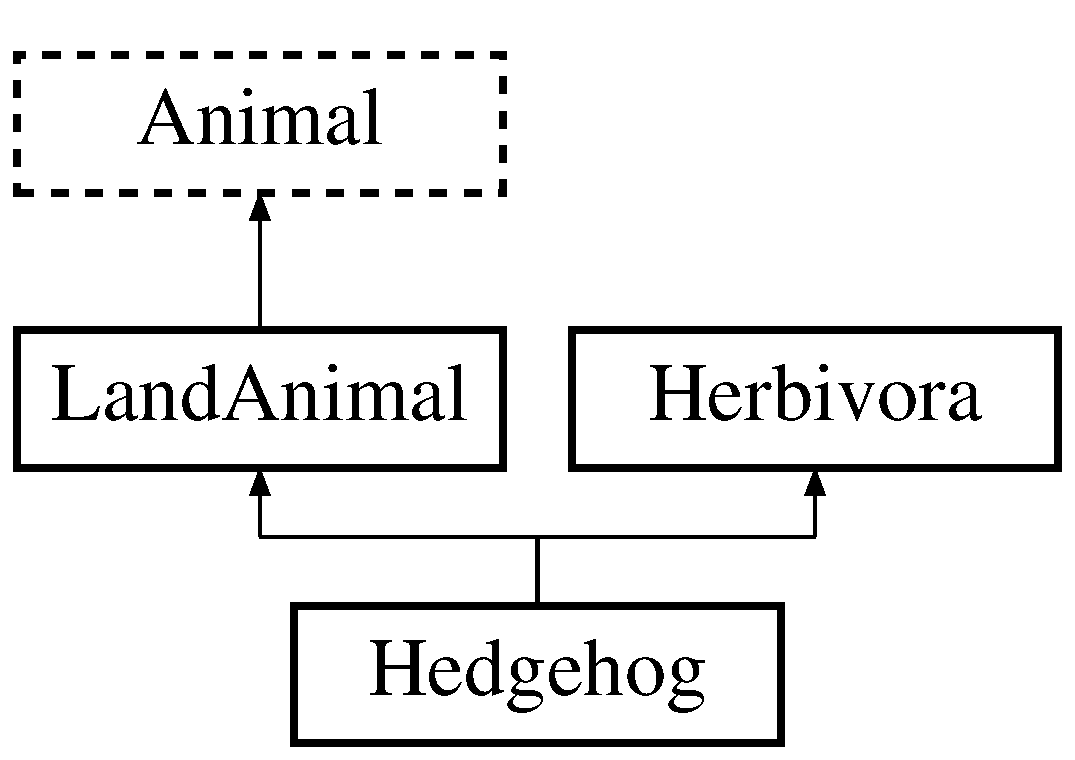
\includegraphics[height=3.000000cm]{classHedgehog}
\end{center}
\end{figure}
\subsection*{Public Member Functions}
\begin{DoxyCompactItemize}
\item 
\hyperlink{classHedgehog_a0b832eb1f52c1c32a236706b5b560c3a}{Hedgehog} (int \-\_\-x, int \-\_\-y)
\begin{DoxyCompactList}\small\item\em Constructor. \end{DoxyCompactList}\item 
\hypertarget{classHedgehog_abc3df9705fd702c76bc3269b2ce9956b}{\hyperlink{classHedgehog_abc3df9705fd702c76bc3269b2ce9956b}{$\sim$\-Hedgehog} ()}\label{classHedgehog_abc3df9705fd702c76bc3269b2ce9956b}

\begin{DoxyCompactList}\small\item\em Destructor. \end{DoxyCompactList}\item 
\hypertarget{classHedgehog_ab8bbcff5c339a144eba0e6810d380512}{void \hyperlink{classHedgehog_ab8bbcff5c339a144eba0e6810d380512}{add\-Bobot} ()}\label{classHedgehog_ab8bbcff5c339a144eba0e6810d380512}

\begin{DoxyCompactList}\small\item\em Menambahkan bobot satu satuan. \end{DoxyCompactList}\item 
int \hyperlink{classHedgehog_a4756f496e554eb53fe9fe42af5d4c359}{get\-Bobot} ()
\begin{DoxyCompactList}\small\item\em Mendapatkan nilai bobot dari \hyperlink{classHedgehog}{Hedgehog}. \end{DoxyCompactList}\item 
char \hyperlink{classHedgehog_aa6dd18c288110a508502abb7c180fd7c}{get\-Simbol} ()
\begin{DoxyCompactList}\small\item\em Mendapatkan simbol dari \hyperlink{classHedgehog}{Hedgehog}. \end{DoxyCompactList}\item 
string \hyperlink{classHedgehog_a36e1421838e26fc245649161b2dc97d3}{get\-Musuh} (int i)
\begin{DoxyCompactList}\small\item\em Mendapatkan musuh ke i dari \hyperlink{classHedgehog}{Hedgehog} Musuh merupakan \hyperlink{classAnimal}{Animal} lain yang tidak bisa tinggal dalam satu kandang dengan \hyperlink{classHedgehog}{Hedgehog}. \end{DoxyCompactList}\item 
string \hyperlink{classHedgehog_aa3d9dacd74c2150b6254b8edff36fb3a}{interact} ()
\begin{DoxyCompactList}\small\item\em Mendapatkan reaksi \hyperlink{classHedgehog}{Hedgehog} saat berinteraksi dengan pengunjung. \end{DoxyCompactList}\item 
string \hyperlink{classHedgehog_a1b17920e9c635183e72264f234f1485a}{get\-Tipe\-Animal} ()
\begin{DoxyCompactList}\small\item\em Mendapatkan tipe \hyperlink{classAnimal}{Animal} (nama spesies) \end{DoxyCompactList}\end{DoxyCompactItemize}
\subsection*{Protected Attributes}
\begin{DoxyCompactItemize}
\item 
\hypertarget{classHedgehog_aa5f07f95b0736a6cfe31746faa11e37b}{const string {\bfseries tipe\-Animal} = \char`\"{}hedgehog\char`\"{}}\label{classHedgehog_aa5f07f95b0736a6cfe31746faa11e37b}

\item 
\hypertarget{classHedgehog_add639a985cb123669869f7af7045f707}{const char {\bfseries simbol} = 'h'}\label{classHedgehog_add639a985cb123669869f7af7045f707}

\item 
\hypertarget{classHedgehog_a69457c4b580174ab0ea23735cd0303a0}{int {\bfseries bobot}}\label{classHedgehog_a69457c4b580174ab0ea23735cd0303a0}

\item 
\hypertarget{classHedgehog_a5ab460e899132b14c4dbcd3555a163b5}{string $\ast$ {\bfseries musuh}}\label{classHedgehog_a5ab460e899132b14c4dbcd3555a163b5}

\end{DoxyCompactItemize}


\subsection{Detailed Description}
Merupakan \hyperlink{classAnimal}{Animal} yang tinggal di darat dan merupakan \hyperlink{classHerbivora}{Herbivora} 

\subsection{Constructor \& Destructor Documentation}
\hypertarget{classHedgehog_a0b832eb1f52c1c32a236706b5b560c3a}{\index{Hedgehog@{Hedgehog}!Hedgehog@{Hedgehog}}
\index{Hedgehog@{Hedgehog}!Hedgehog@{Hedgehog}}
\subsubsection[{Hedgehog}]{\setlength{\rightskip}{0pt plus 5cm}Hedgehog\-::\-Hedgehog (
\begin{DoxyParamCaption}
\item[{int}]{\-\_\-x, }
\item[{int}]{\-\_\-y}
\end{DoxyParamCaption}
)}}\label{classHedgehog_a0b832eb1f52c1c32a236706b5b560c3a}


Constructor. 


\begin{DoxyParams}{Parameters}
{\em \-\_\-x} & posisi x awal \hyperlink{classHedgehog}{Hedgehog} \\
\hline
{\em \-\_\-y} & posisi y awal \hyperlink{classHedgehog}{Hedgehog} \\
\hline
\end{DoxyParams}


\subsection{Member Function Documentation}
\hypertarget{classHedgehog_a4756f496e554eb53fe9fe42af5d4c359}{\index{Hedgehog@{Hedgehog}!get\-Bobot@{get\-Bobot}}
\index{get\-Bobot@{get\-Bobot}!Hedgehog@{Hedgehog}}
\subsubsection[{get\-Bobot}]{\setlength{\rightskip}{0pt plus 5cm}int Hedgehog\-::get\-Bobot (
\begin{DoxyParamCaption}
{}
\end{DoxyParamCaption}
)\hspace{0.3cm}{\ttfamily [virtual]}}}\label{classHedgehog_a4756f496e554eb53fe9fe42af5d4c359}


Mendapatkan nilai bobot dari \hyperlink{classHedgehog}{Hedgehog}. 

\begin{DoxyReturn}{Returns}
bobot 
\end{DoxyReturn}


Implements \hyperlink{classAnimal}{Animal}.

\hypertarget{classHedgehog_a36e1421838e26fc245649161b2dc97d3}{\index{Hedgehog@{Hedgehog}!get\-Musuh@{get\-Musuh}}
\index{get\-Musuh@{get\-Musuh}!Hedgehog@{Hedgehog}}
\subsubsection[{get\-Musuh}]{\setlength{\rightskip}{0pt plus 5cm}string Hedgehog\-::get\-Musuh (
\begin{DoxyParamCaption}
\item[{int}]{i}
\end{DoxyParamCaption}
)\hspace{0.3cm}{\ttfamily [virtual]}}}\label{classHedgehog_a36e1421838e26fc245649161b2dc97d3}


Mendapatkan musuh ke i dari \hyperlink{classHedgehog}{Hedgehog} Musuh merupakan \hyperlink{classAnimal}{Animal} lain yang tidak bisa tinggal dalam satu kandang dengan \hyperlink{classHedgehog}{Hedgehog}. 

\begin{DoxyReturn}{Returns}
musuh\mbox{[}i\mbox{]} 
\end{DoxyReturn}


Implements \hyperlink{classAnimal}{Animal}.

\hypertarget{classHedgehog_aa6dd18c288110a508502abb7c180fd7c}{\index{Hedgehog@{Hedgehog}!get\-Simbol@{get\-Simbol}}
\index{get\-Simbol@{get\-Simbol}!Hedgehog@{Hedgehog}}
\subsubsection[{get\-Simbol}]{\setlength{\rightskip}{0pt plus 5cm}char Hedgehog\-::get\-Simbol (
\begin{DoxyParamCaption}
{}
\end{DoxyParamCaption}
)\hspace{0.3cm}{\ttfamily [virtual]}}}\label{classHedgehog_aa6dd18c288110a508502abb7c180fd7c}


Mendapatkan simbol dari \hyperlink{classHedgehog}{Hedgehog}. 

\begin{DoxyReturn}{Returns}
simbol 
\end{DoxyReturn}


Implements \hyperlink{classAnimal}{Animal}.

\hypertarget{classHedgehog_a1b17920e9c635183e72264f234f1485a}{\index{Hedgehog@{Hedgehog}!get\-Tipe\-Animal@{get\-Tipe\-Animal}}
\index{get\-Tipe\-Animal@{get\-Tipe\-Animal}!Hedgehog@{Hedgehog}}
\subsubsection[{get\-Tipe\-Animal}]{\setlength{\rightskip}{0pt plus 5cm}string Hedgehog\-::get\-Tipe\-Animal (
\begin{DoxyParamCaption}
{}
\end{DoxyParamCaption}
)\hspace{0.3cm}{\ttfamily [virtual]}}}\label{classHedgehog_a1b17920e9c635183e72264f234f1485a}


Mendapatkan tipe \hyperlink{classAnimal}{Animal} (nama spesies) 

\begin{DoxyReturn}{Returns}
tipe\-Animal 
\end{DoxyReturn}


Implements \hyperlink{classLandAnimal}{Land\-Animal}.

\hypertarget{classHedgehog_aa3d9dacd74c2150b6254b8edff36fb3a}{\index{Hedgehog@{Hedgehog}!interact@{interact}}
\index{interact@{interact}!Hedgehog@{Hedgehog}}
\subsubsection[{interact}]{\setlength{\rightskip}{0pt plus 5cm}string Hedgehog\-::interact (
\begin{DoxyParamCaption}
{}
\end{DoxyParamCaption}
)\hspace{0.3cm}{\ttfamily [virtual]}}}\label{classHedgehog_aa3d9dacd74c2150b6254b8edff36fb3a}


Mendapatkan reaksi \hyperlink{classHedgehog}{Hedgehog} saat berinteraksi dengan pengunjung. 

\begin{DoxyReturn}{Returns}
\char`\"{}duriduri\char`\"{} 
\end{DoxyReturn}


Implements \hyperlink{classLandAnimal}{Land\-Animal}.



The documentation for this class was generated from the following files\-:\begin{DoxyCompactItemize}
\item 
Hedgehog.\-h\item 
Hedgehog.\-cpp\end{DoxyCompactItemize}

\hypertarget{classHerbivora}{\section{Herbivora Class Reference}
\label{classHerbivora}\index{Herbivora@{Herbivora}}
}


{\ttfamily \#include $<$Herbivora.\-h$>$}

Inheritance diagram for Herbivora\-:\begin{figure}[H]
\begin{center}
\leavevmode
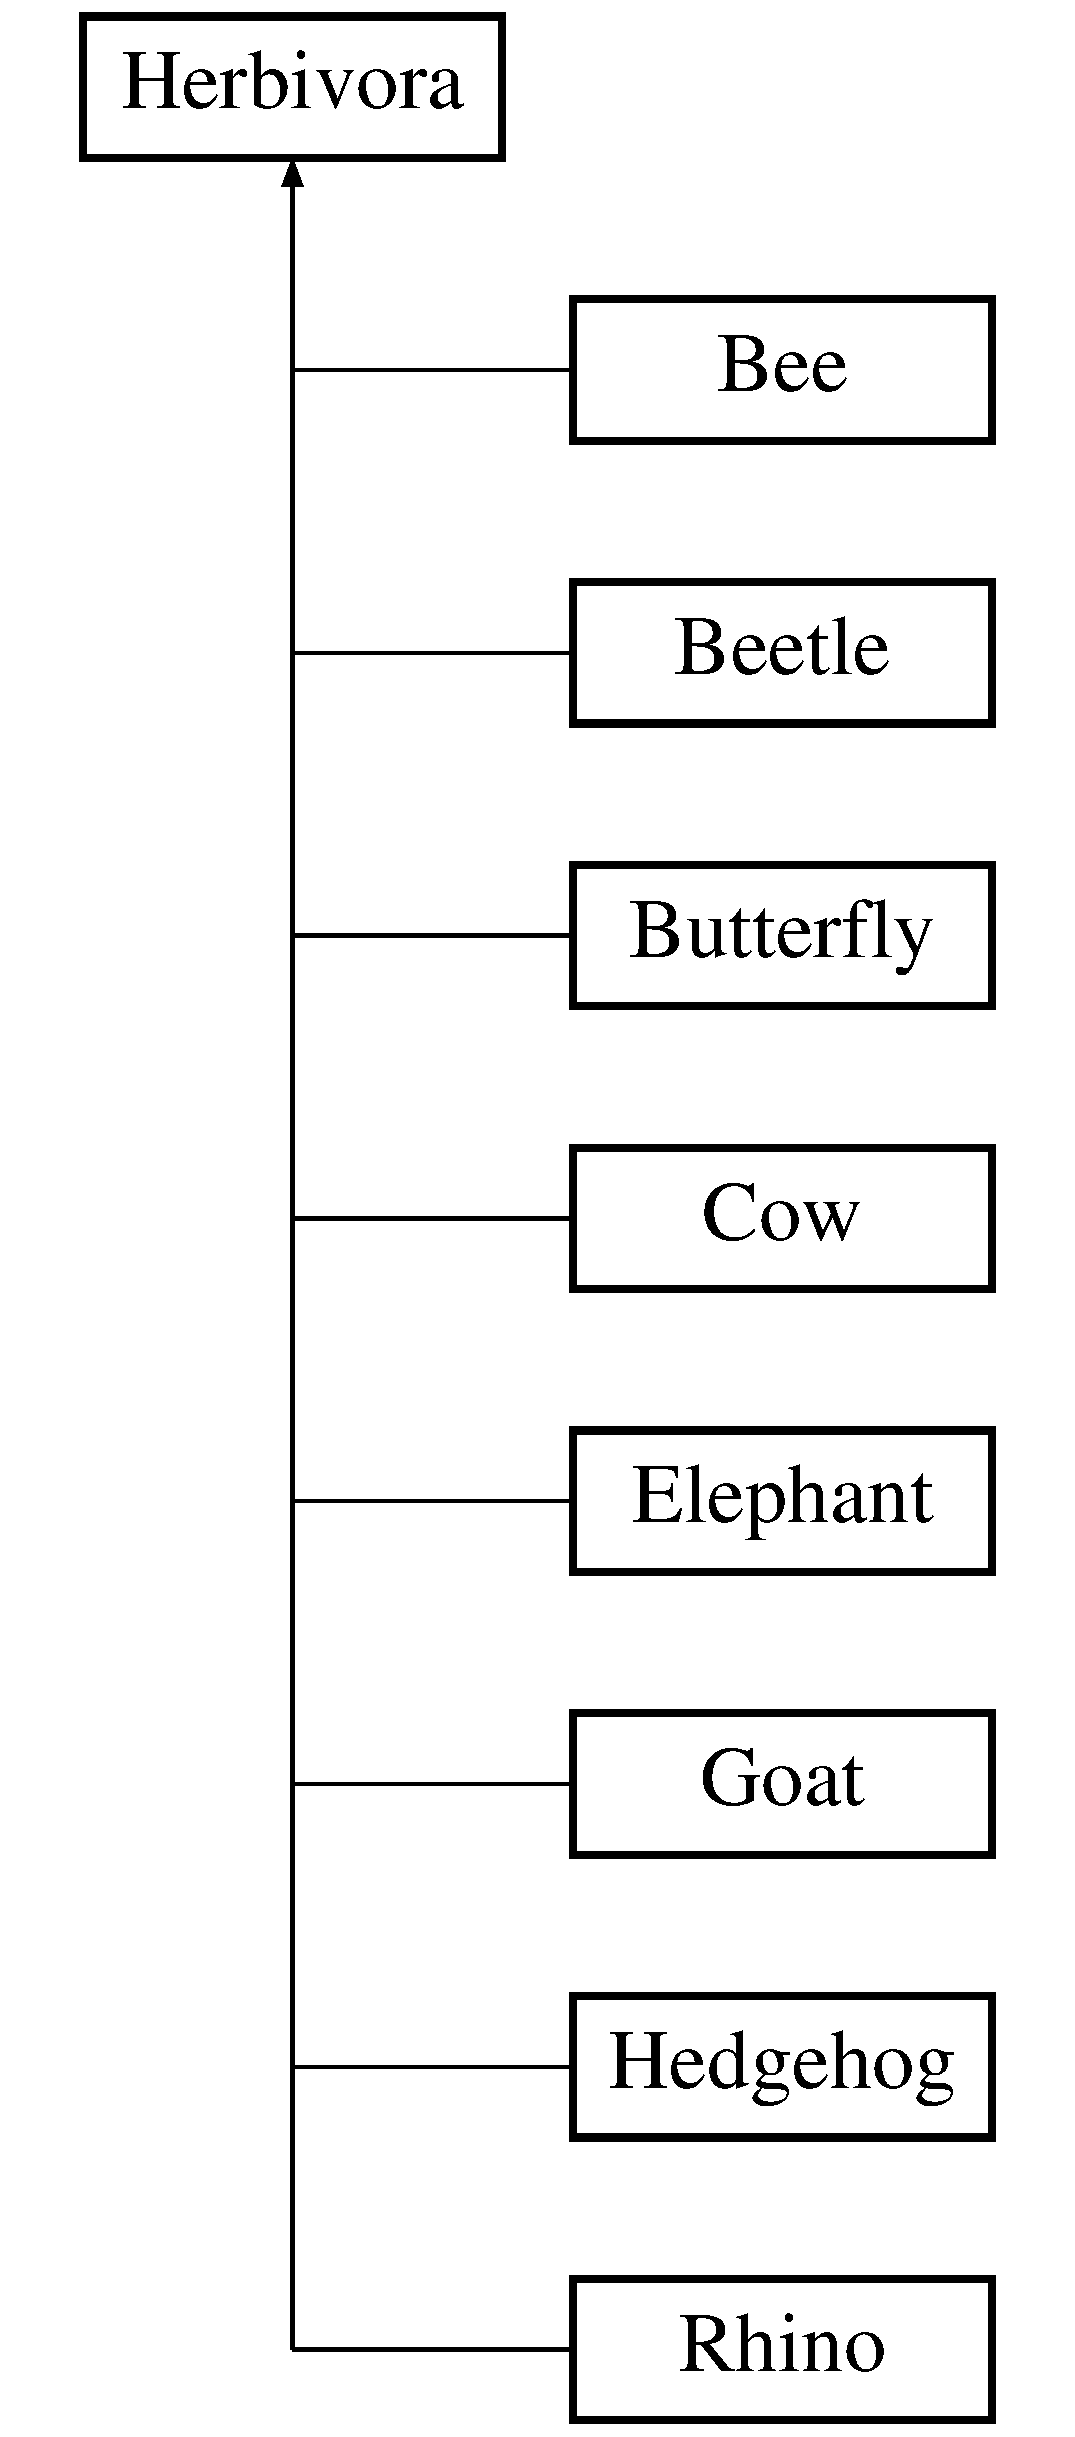
\includegraphics[height=9.000000cm]{classHerbivora}
\end{center}
\end{figure}
\subsection*{Protected Attributes}
\begin{DoxyCompactItemize}
\item 
\hypertarget{classHerbivora_a821e0f6807a16249d4c1d00924aa1d2d}{const string {\bfseries tipe\-Makanan} =\char`\"{}herbivora\char`\"{}}\label{classHerbivora_a821e0f6807a16249d4c1d00924aa1d2d}

\end{DoxyCompactItemize}


\subsection{Detailed Description}
\hyperlink{classHerbivora}{Herbivora} merupakan tipe \hyperlink{classAnimal}{Animal} pemakan tumbuhan 

The documentation for this class was generated from the following file\-:\begin{DoxyCompactItemize}
\item 
Herbivora.\-h\end{DoxyCompactItemize}

\hypertarget{classKarnivora}{\section{Karnivora Class Reference}
\label{classKarnivora}\index{Karnivora@{Karnivora}}
}


{\ttfamily \#include $<$Karnivora.\-h$>$}

Inheritance diagram for Karnivora\-:\begin{figure}[H]
\begin{center}
\leavevmode
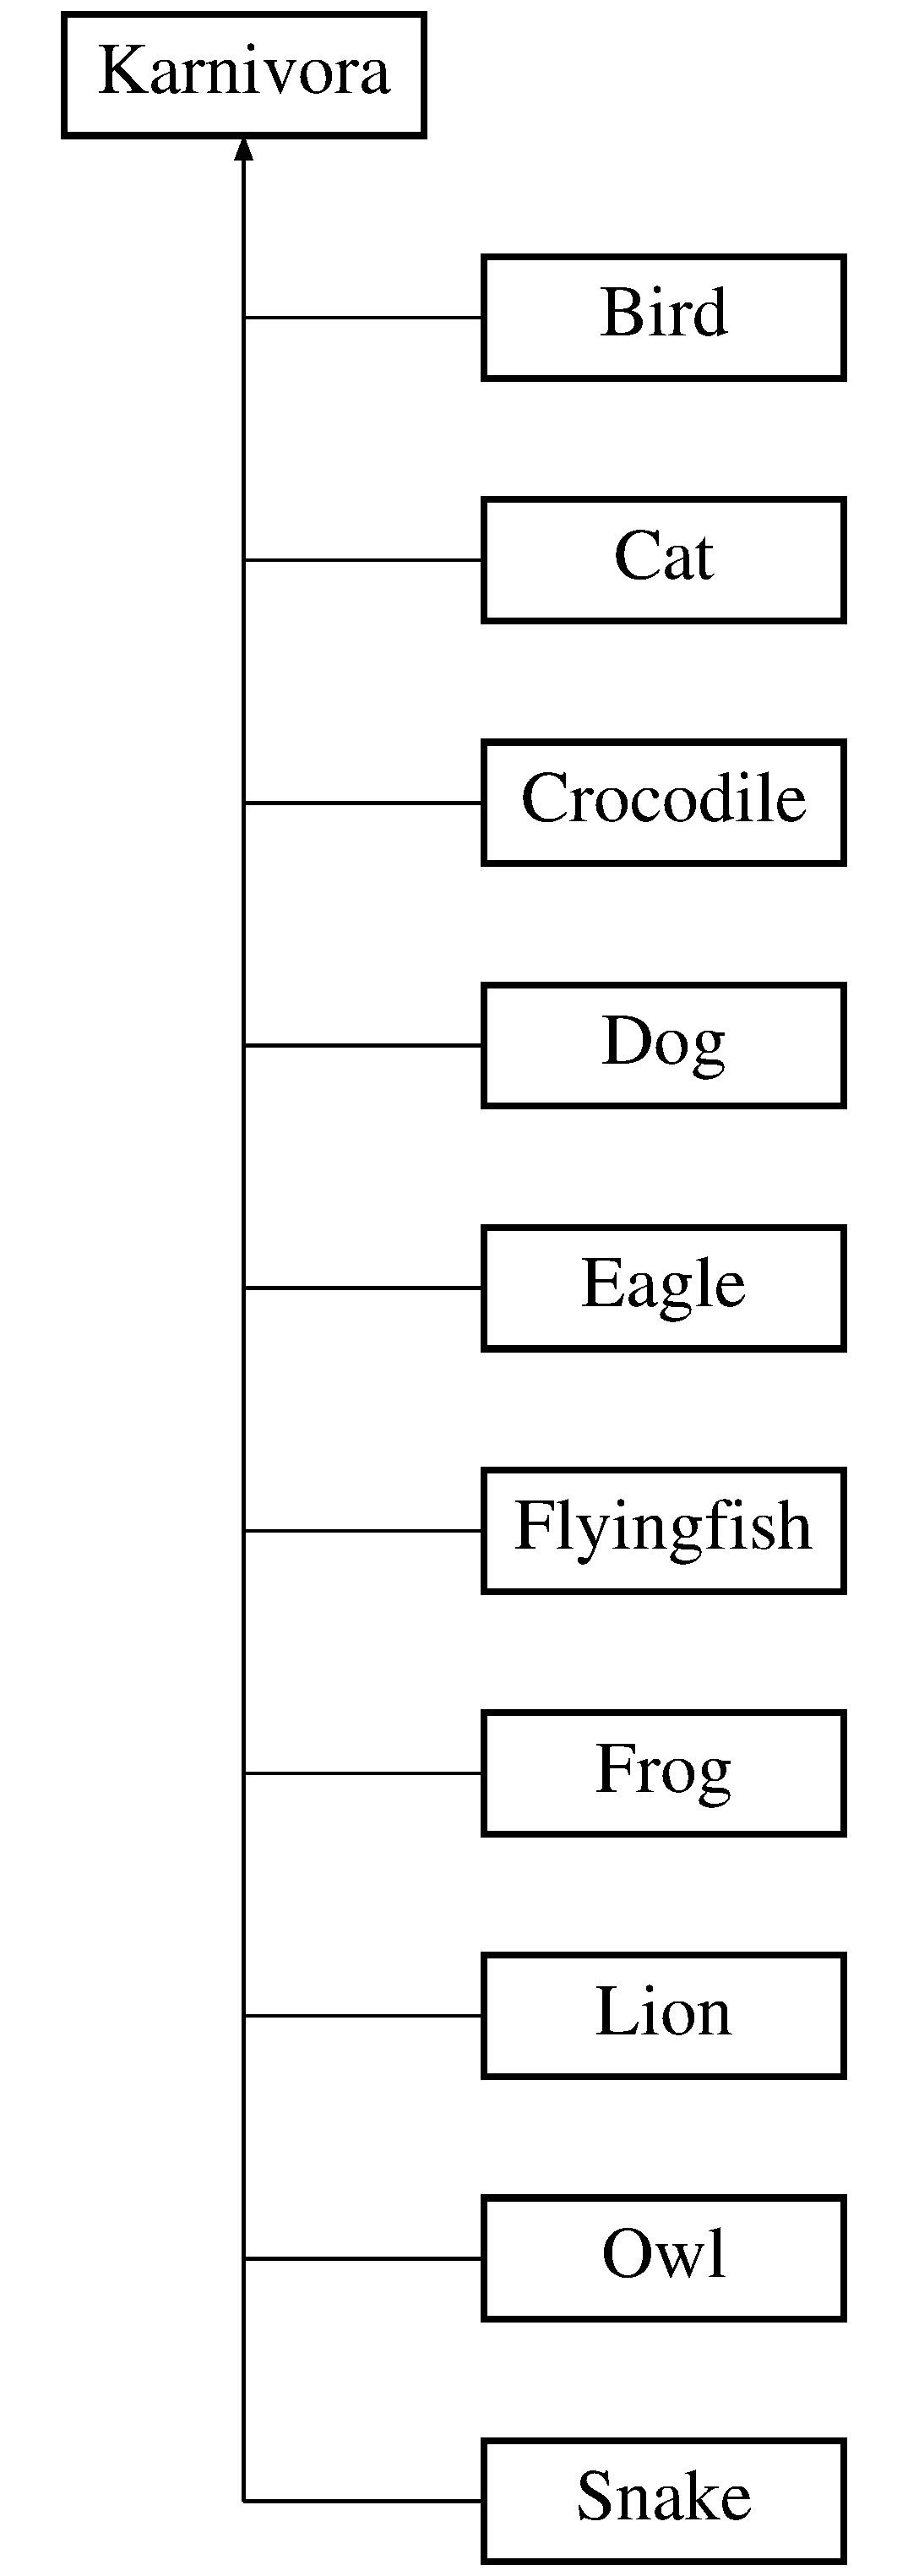
\includegraphics[height=11.000000cm]{classKarnivora}
\end{center}
\end{figure}
\subsection*{Protected Attributes}
\begin{DoxyCompactItemize}
\item 
\hypertarget{classKarnivora_a2f994f23bc64dd353d068b54a899b4c2}{const string {\bfseries tipe\-Makanan} =\char`\"{}karnivora\char`\"{}}\label{classKarnivora_a2f994f23bc64dd353d068b54a899b4c2}

\end{DoxyCompactItemize}


\subsection{Detailed Description}
\hyperlink{classKarnivora}{Karnivora} merupakan tipe \hyperlink{classAnimal}{Animal} pemakan daging 

The documentation for this class was generated from the following file\-:\begin{DoxyCompactItemize}
\item 
Karnivora.\-h\end{DoxyCompactItemize}

\hypertarget{classLandAnimal}{\section{Land\-Animal Class Reference}
\label{classLandAnimal}\index{Land\-Animal@{Land\-Animal}}
}
Inheritance diagram for Land\-Animal\-:\begin{figure}[H]
\begin{center}
\leavevmode
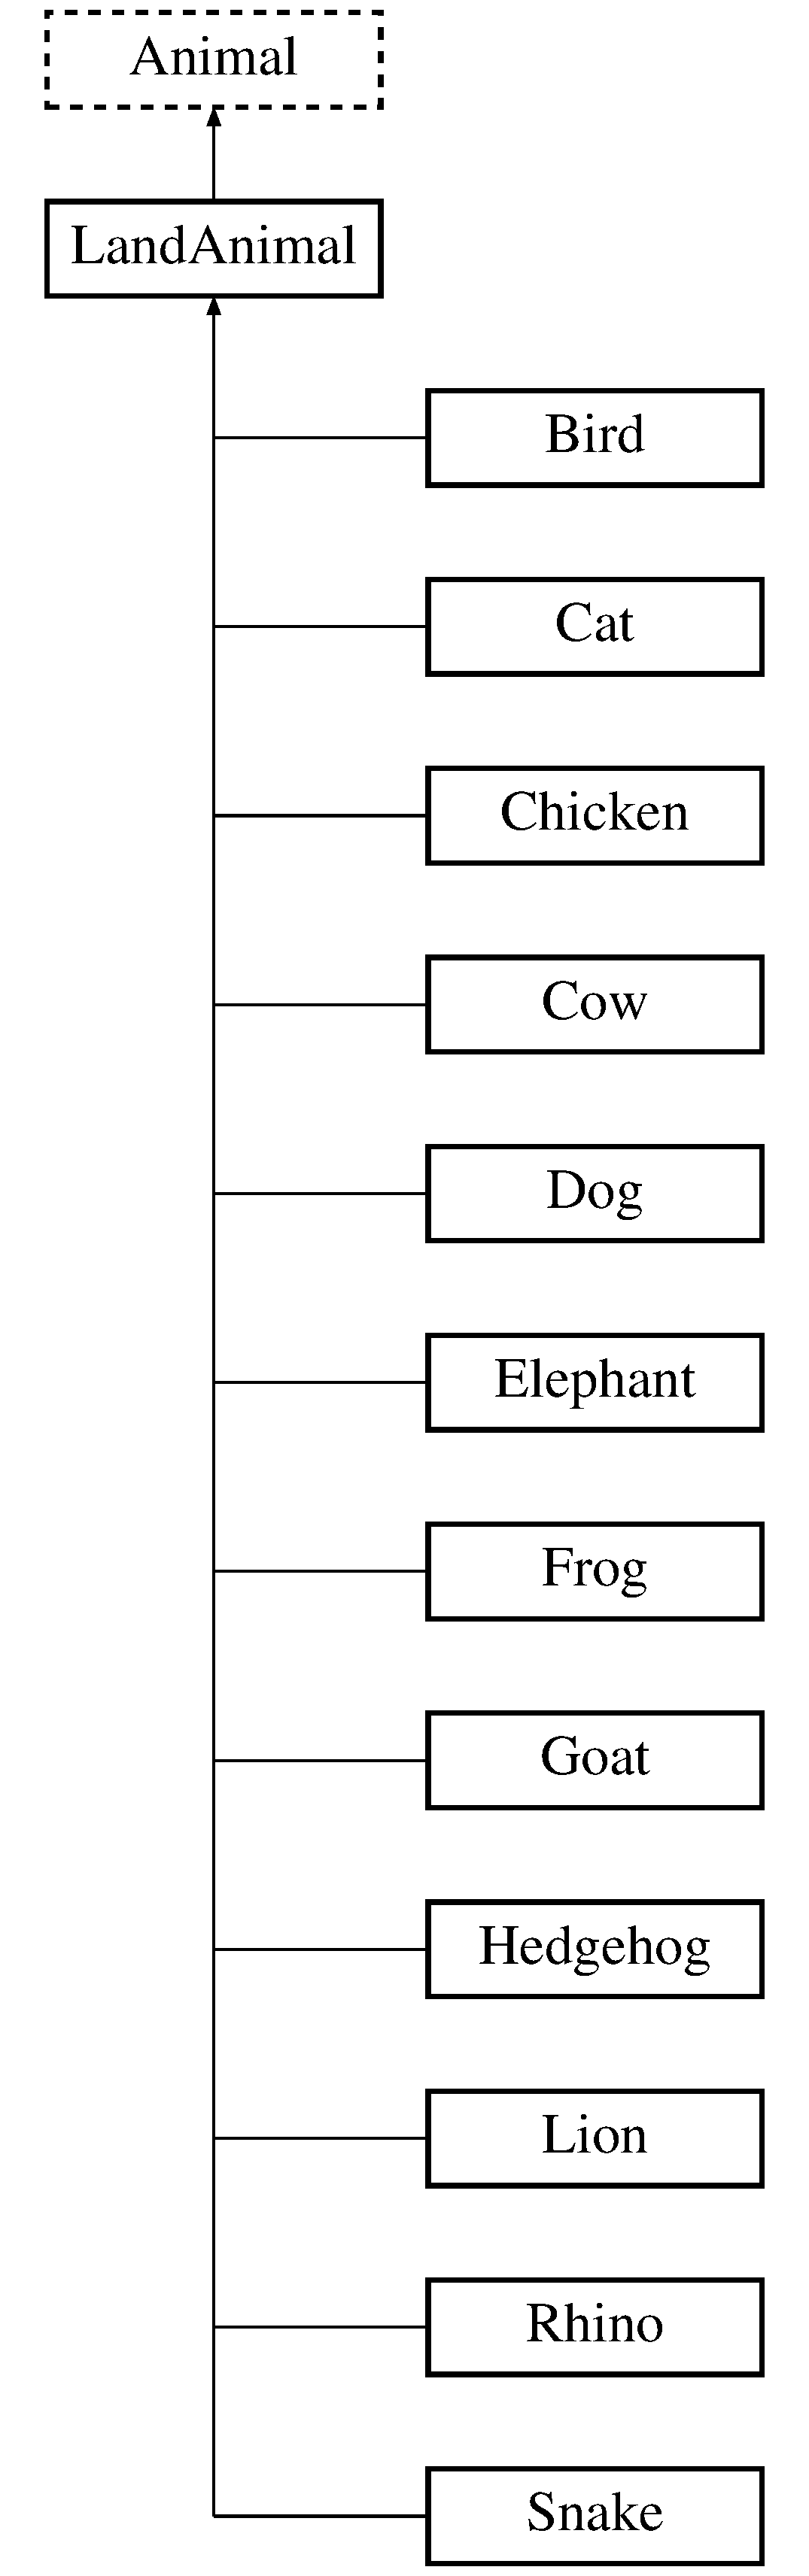
\includegraphics[height=12.000000cm]{classLandAnimal}
\end{center}
\end{figure}
\subsection*{Public Member Functions}
\begin{DoxyCompactItemize}
\item 
\hypertarget{classLandAnimal_a93f431da1888f6b8397492c70ff5c465}{{\bfseries Land\-Animal} (int, int)}\label{classLandAnimal_a93f431da1888f6b8397492c70ff5c465}

\item 
\hypertarget{classLandAnimal_a30d3d693ec1a1d7589a75e93c0efcef7}{{\bfseries Land\-Animal} (const \hyperlink{classLandAnimal}{Land\-Animal} \&)}\label{classLandAnimal_a30d3d693ec1a1d7589a75e93c0efcef7}

\item 
\hypertarget{classLandAnimal_a6875179adbd1d991ac0615c7756af61e}{virtual string {\bfseries interact} ()=0}\label{classLandAnimal_a6875179adbd1d991ac0615c7756af61e}

\item 
\hypertarget{classLandAnimal_a8bba1c5493ba6a5618787b2aec0b128b}{virtual string {\bfseries get\-Tipe\-Habitat} ()}\label{classLandAnimal_a8bba1c5493ba6a5618787b2aec0b128b}

\item 
\hypertarget{classLandAnimal_aca2d4efdbfd3a7577d293f3caf9b650d}{virtual string {\bfseries get\-Tipe\-Animal} ()=0}\label{classLandAnimal_aca2d4efdbfd3a7577d293f3caf9b650d}

\end{DoxyCompactItemize}
\subsection*{Protected Attributes}
\begin{DoxyCompactItemize}
\item 
\hypertarget{classLandAnimal_a5752a73759922767a929a6ca1bcfc017}{const string {\bfseries tipe\-Habitat} = \char`\"{}land\char`\"{}}\label{classLandAnimal_a5752a73759922767a929a6ca1bcfc017}

\end{DoxyCompactItemize}


The documentation for this class was generated from the following files\-:\begin{DoxyCompactItemize}
\item 
Land\-Animal.\-h\item 
Land\-Animal.\-cpp\end{DoxyCompactItemize}

\hypertarget{classLandHabitat}{\section{Land\-Habitat Class Reference}
\label{classLandHabitat}\index{Land\-Habitat@{Land\-Habitat}}
}


{\ttfamily \#include $<$Land\-Habitat.\-h$>$}

Inheritance diagram for Land\-Habitat\-:\begin{figure}[H]
\begin{center}
\leavevmode
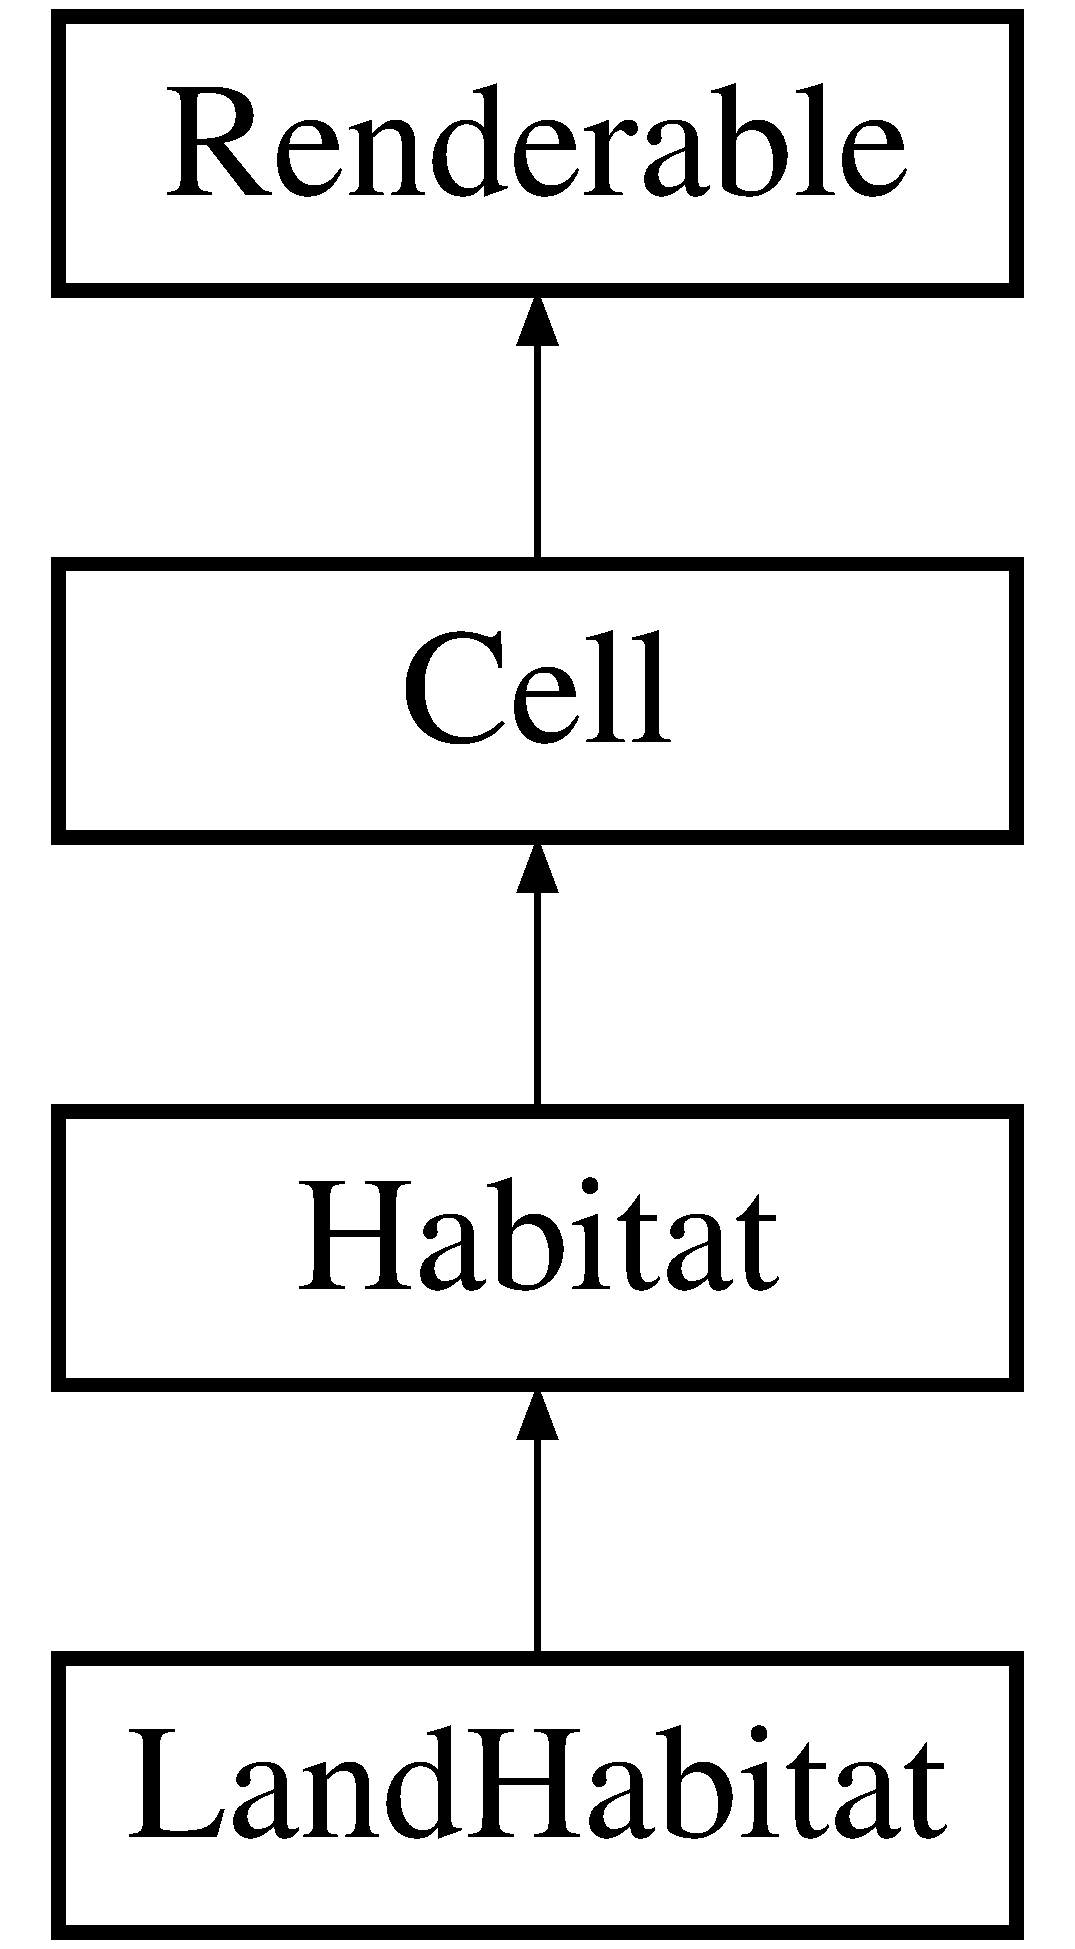
\includegraphics[height=4.000000cm]{classLandHabitat}
\end{center}
\end{figure}
\subsection*{Public Member Functions}
\begin{DoxyCompactItemize}
\item 
\hyperlink{classLandHabitat_aad78cb4d516dd40205b2541cd03efd9d}{Land\-Habitat} (int x, int y, char s)
\begin{DoxyCompactList}\small\item\em Constructor. \end{DoxyCompactList}\item 
string \hyperlink{classLandHabitat_a51ad769f1682ec5b45bcd8839e854575}{get\-Tipe} ()
\begin{DoxyCompactList}\small\item\em Mendapatkan tipe \hyperlink{classCell}{Cell}. \end{DoxyCompactList}\end{DoxyCompactItemize}


\subsection{Detailed Description}
Kelas \hyperlink{classLandHabitat}{Land\-Habitat} adalah kelas turunan dari \hyperlink{classHabitat}{Habitat} 

\subsection{Constructor \& Destructor Documentation}
\hypertarget{classLandHabitat_aad78cb4d516dd40205b2541cd03efd9d}{\index{Land\-Habitat@{Land\-Habitat}!Land\-Habitat@{Land\-Habitat}}
\index{Land\-Habitat@{Land\-Habitat}!LandHabitat@{Land\-Habitat}}
\subsubsection[{Land\-Habitat}]{\setlength{\rightskip}{0pt plus 5cm}Land\-Habitat\-::\-Land\-Habitat (
\begin{DoxyParamCaption}
\item[{int}]{x, }
\item[{int}]{y, }
\item[{char}]{s}
\end{DoxyParamCaption}
)}}\label{classLandHabitat_aad78cb4d516dd40205b2541cd03efd9d}


Constructor. 


\begin{DoxyParams}{Parameters}
{\em x} & Indeks baris \\
\hline
{\em y} & Indeks kolom \\
\hline
{\em s} & Simbol \\
\hline
\end{DoxyParams}


\subsection{Member Function Documentation}
\hypertarget{classLandHabitat_a51ad769f1682ec5b45bcd8839e854575}{\index{Land\-Habitat@{Land\-Habitat}!get\-Tipe@{get\-Tipe}}
\index{get\-Tipe@{get\-Tipe}!LandHabitat@{Land\-Habitat}}
\subsubsection[{get\-Tipe}]{\setlength{\rightskip}{0pt plus 5cm}string Land\-Habitat\-::get\-Tipe (
\begin{DoxyParamCaption}
{}
\end{DoxyParamCaption}
)\hspace{0.3cm}{\ttfamily [virtual]}}}\label{classLandHabitat_a51ad769f1682ec5b45bcd8839e854575}


Mendapatkan tipe \hyperlink{classCell}{Cell}. 

\begin{DoxyReturn}{Returns}
tipe 
\end{DoxyReturn}


Implements \hyperlink{classHabitat_a4c8164f06a0a32ca6c7f465380b31ac0}{Habitat}.



The documentation for this class was generated from the following files\-:\begin{DoxyCompactItemize}
\item 
Land\-Habitat.\-h\item 
Land\-Habitat.\-cpp\end{DoxyCompactItemize}

\hypertarget{classLion}{\section{Lion Class Reference}
\label{classLion}\index{Lion@{Lion}}
}


{\ttfamily \#include $<$Lion.\-h$>$}

Inheritance diagram for Lion\-:\begin{figure}[H]
\begin{center}
\leavevmode
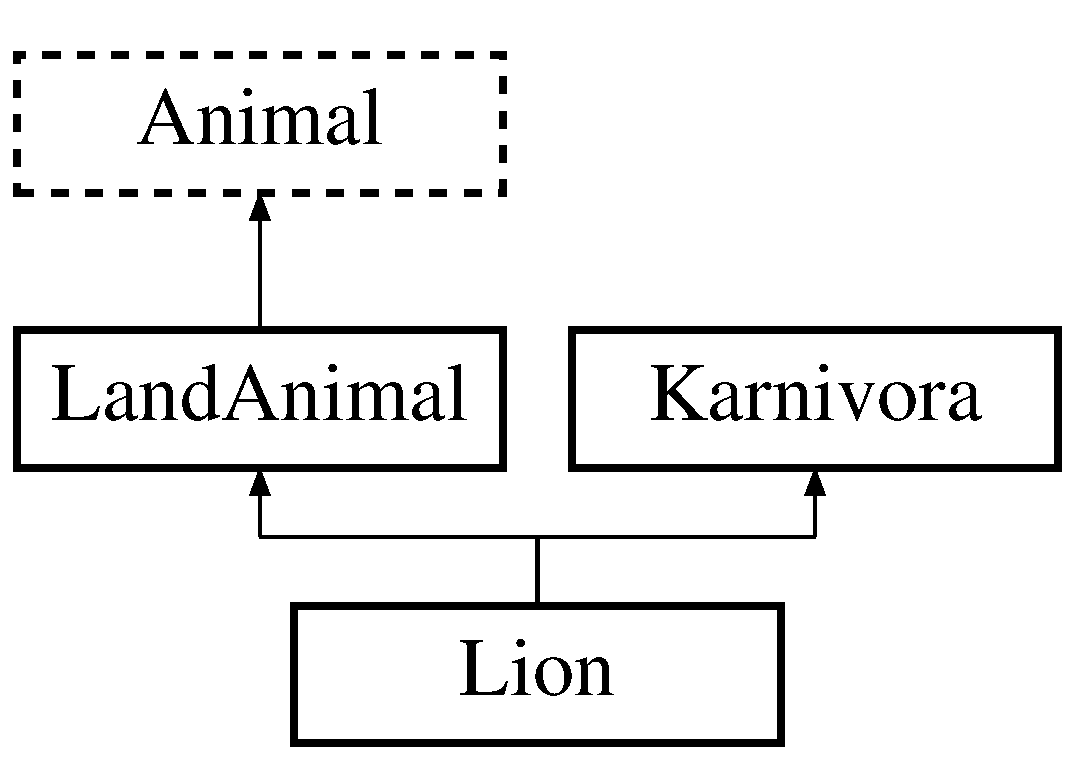
\includegraphics[height=3.000000cm]{classLion}
\end{center}
\end{figure}
\subsection*{Public Member Functions}
\begin{DoxyCompactItemize}
\item 
\hyperlink{classLion_aff2734ad945e35069dab03493aa34e51}{Lion} (int \-\_\-x, int \-\_\-y)
\begin{DoxyCompactList}\small\item\em Constructor. \end{DoxyCompactList}\item 
\hypertarget{classLion_add3b70c968c9382d00f25f5d148e590f}{\hyperlink{classLion_add3b70c968c9382d00f25f5d148e590f}{$\sim$\-Lion} ()}\label{classLion_add3b70c968c9382d00f25f5d148e590f}

\begin{DoxyCompactList}\small\item\em Destructor. \end{DoxyCompactList}\item 
\hypertarget{classLion_aff4d22a6a78a3d029c612c92bd878e7a}{void \hyperlink{classLion_aff4d22a6a78a3d029c612c92bd878e7a}{add\-Bobot} ()}\label{classLion_aff4d22a6a78a3d029c612c92bd878e7a}

\begin{DoxyCompactList}\small\item\em Menambahkan bobot satu satuan. \end{DoxyCompactList}\item 
int \hyperlink{classLion_a039685367875d1cdf4779dce5232edec}{get\-Bobot} ()
\begin{DoxyCompactList}\small\item\em Mendapatkan nilai bobot dari \hyperlink{classLion}{Lion}. \end{DoxyCompactList}\item 
char \hyperlink{classLion_a91396289e60961249390e04bddca1f33}{get\-Simbol} ()
\begin{DoxyCompactList}\small\item\em Mendapatkan simbol dari \hyperlink{classLion}{Lion}. \end{DoxyCompactList}\item 
string \hyperlink{classLion_a6afed6b04ba30683547b43d12db22602}{get\-Musuh} (int i)
\begin{DoxyCompactList}\small\item\em Mendapatkan musuh ke i dari \hyperlink{classLion}{Lion} Musuh merupakan \hyperlink{classAnimal}{Animal} lain yang tidak bisa tinggal dalam satu kandang dengan \hyperlink{classLion}{Lion}. \end{DoxyCompactList}\item 
string \hyperlink{classLion_a5ec3e7aa8b23aabab1c83fdf9e7d0edc}{interact} ()
\begin{DoxyCompactList}\small\item\em Mendapatkan reaksi \hyperlink{classLion}{Lion} saat berinteraksi dengan pengunjung. \end{DoxyCompactList}\item 
string \hyperlink{classLion_ab84e7ce8adc60b918947a03274574274}{get\-Tipe\-Animal} ()
\begin{DoxyCompactList}\small\item\em Mendapatkan tipe \hyperlink{classAnimal}{Animal} (nama spesies) \end{DoxyCompactList}\end{DoxyCompactItemize}
\subsection*{Protected Attributes}
\begin{DoxyCompactItemize}
\item 
\hypertarget{classLion_adcc07efde3d3b032c3c46b152fbdbff0}{const string {\bfseries tipe\-Animal} = \char`\"{}lion\char`\"{}}\label{classLion_adcc07efde3d3b032c3c46b152fbdbff0}

\item 
\hypertarget{classLion_ad68fc66ed2526913a48204c498b15640}{const char {\bfseries simbol} = 'l'}\label{classLion_ad68fc66ed2526913a48204c498b15640}

\item 
\hypertarget{classLion_a8b06cc2870dd127c43a91a618cc2a14c}{int {\bfseries bobot}}\label{classLion_a8b06cc2870dd127c43a91a618cc2a14c}

\item 
\hypertarget{classLion_ad44a83ee9b4e2f2b47b2bb2d85f9d648}{string $\ast$ {\bfseries musuh}}\label{classLion_ad44a83ee9b4e2f2b47b2bb2d85f9d648}

\end{DoxyCompactItemize}


\subsection{Detailed Description}
Merupakan \hyperlink{classAnimal}{Animal} yang tinggal di darat dan merupakan \hyperlink{classKarnivora}{Karnivora} 

\subsection{Constructor \& Destructor Documentation}
\hypertarget{classLion_aff2734ad945e35069dab03493aa34e51}{\index{Lion@{Lion}!Lion@{Lion}}
\index{Lion@{Lion}!Lion@{Lion}}
\subsubsection[{Lion}]{\setlength{\rightskip}{0pt plus 5cm}Lion\-::\-Lion (
\begin{DoxyParamCaption}
\item[{int}]{\-\_\-x, }
\item[{int}]{\-\_\-y}
\end{DoxyParamCaption}
)}}\label{classLion_aff2734ad945e35069dab03493aa34e51}


Constructor. 


\begin{DoxyParams}{Parameters}
{\em \-\_\-x} & posisi x awal \hyperlink{classLion}{Lion} \\
\hline
{\em \-\_\-y} & posisi y awal \hyperlink{classLion}{Lion} \\
\hline
\end{DoxyParams}


\subsection{Member Function Documentation}
\hypertarget{classLion_a039685367875d1cdf4779dce5232edec}{\index{Lion@{Lion}!get\-Bobot@{get\-Bobot}}
\index{get\-Bobot@{get\-Bobot}!Lion@{Lion}}
\subsubsection[{get\-Bobot}]{\setlength{\rightskip}{0pt plus 5cm}int Lion\-::get\-Bobot (
\begin{DoxyParamCaption}
{}
\end{DoxyParamCaption}
)\hspace{0.3cm}{\ttfamily [virtual]}}}\label{classLion_a039685367875d1cdf4779dce5232edec}


Mendapatkan nilai bobot dari \hyperlink{classLion}{Lion}. 

\begin{DoxyReturn}{Returns}
bobot 
\end{DoxyReturn}


Implements \hyperlink{classAnimal}{Animal}.

\hypertarget{classLion_a6afed6b04ba30683547b43d12db22602}{\index{Lion@{Lion}!get\-Musuh@{get\-Musuh}}
\index{get\-Musuh@{get\-Musuh}!Lion@{Lion}}
\subsubsection[{get\-Musuh}]{\setlength{\rightskip}{0pt plus 5cm}string Lion\-::get\-Musuh (
\begin{DoxyParamCaption}
\item[{int}]{i}
\end{DoxyParamCaption}
)\hspace{0.3cm}{\ttfamily [virtual]}}}\label{classLion_a6afed6b04ba30683547b43d12db22602}


Mendapatkan musuh ke i dari \hyperlink{classLion}{Lion} Musuh merupakan \hyperlink{classAnimal}{Animal} lain yang tidak bisa tinggal dalam satu kandang dengan \hyperlink{classLion}{Lion}. 

\begin{DoxyReturn}{Returns}
musuh\mbox{[}i\mbox{]} 
\end{DoxyReturn}


Implements \hyperlink{classAnimal}{Animal}.

\hypertarget{classLion_a91396289e60961249390e04bddca1f33}{\index{Lion@{Lion}!get\-Simbol@{get\-Simbol}}
\index{get\-Simbol@{get\-Simbol}!Lion@{Lion}}
\subsubsection[{get\-Simbol}]{\setlength{\rightskip}{0pt plus 5cm}char Lion\-::get\-Simbol (
\begin{DoxyParamCaption}
{}
\end{DoxyParamCaption}
)\hspace{0.3cm}{\ttfamily [virtual]}}}\label{classLion_a91396289e60961249390e04bddca1f33}


Mendapatkan simbol dari \hyperlink{classLion}{Lion}. 

\begin{DoxyReturn}{Returns}
simbol 
\end{DoxyReturn}


Implements \hyperlink{classAnimal}{Animal}.

\hypertarget{classLion_ab84e7ce8adc60b918947a03274574274}{\index{Lion@{Lion}!get\-Tipe\-Animal@{get\-Tipe\-Animal}}
\index{get\-Tipe\-Animal@{get\-Tipe\-Animal}!Lion@{Lion}}
\subsubsection[{get\-Tipe\-Animal}]{\setlength{\rightskip}{0pt plus 5cm}string Lion\-::get\-Tipe\-Animal (
\begin{DoxyParamCaption}
{}
\end{DoxyParamCaption}
)\hspace{0.3cm}{\ttfamily [virtual]}}}\label{classLion_ab84e7ce8adc60b918947a03274574274}


Mendapatkan tipe \hyperlink{classAnimal}{Animal} (nama spesies) 

\begin{DoxyReturn}{Returns}
tipe\-Animal 
\end{DoxyReturn}


Implements \hyperlink{classLandAnimal}{Land\-Animal}.

\hypertarget{classLion_a5ec3e7aa8b23aabab1c83fdf9e7d0edc}{\index{Lion@{Lion}!interact@{interact}}
\index{interact@{interact}!Lion@{Lion}}
\subsubsection[{interact}]{\setlength{\rightskip}{0pt plus 5cm}string Lion\-::interact (
\begin{DoxyParamCaption}
{}
\end{DoxyParamCaption}
)\hspace{0.3cm}{\ttfamily [virtual]}}}\label{classLion_a5ec3e7aa8b23aabab1c83fdf9e7d0edc}


Mendapatkan reaksi \hyperlink{classLion}{Lion} saat berinteraksi dengan pengunjung. 

\begin{DoxyReturn}{Returns}
\char`\"{}auuum\char`\"{} 
\end{DoxyReturn}


Implements \hyperlink{classLandAnimal}{Land\-Animal}.



The documentation for this class was generated from the following files\-:\begin{DoxyCompactItemize}
\item 
Lion.\-h\item 
Lion.\-cpp\end{DoxyCompactItemize}

\hypertarget{classMatrixCell}{\section{Matrix\-Cell Class Reference}
\label{classMatrixCell}\index{Matrix\-Cell@{Matrix\-Cell}}
}


{\ttfamily \#include $<$matrix\-\_\-cell.\-h$>$}

\subsection*{Public Member Functions}
\begin{DoxyCompactItemize}
\item 
\hyperlink{classMatrixCell_aa3193302e7060271c18d5200e9b02bfd}{Matrix\-Cell} (int brs, int kol)
\begin{DoxyCompactList}\small\item\em Constructor Menciptakan \hyperlink{classMatrixCell}{Matrix\-Cell} sebesar brs dan kol. \end{DoxyCompactList}\item 
\hypertarget{classMatrixCell_acd03a072415e3c564107f745139f364b}{\hyperlink{classMatrixCell_acd03a072415e3c564107f745139f364b}{Matrix\-Cell} (const \hyperlink{classMatrixCell}{Matrix\-Cell} \&)}\label{classMatrixCell_acd03a072415e3c564107f745139f364b}

\begin{DoxyCompactList}\small\item\em Copy Constructor. \end{DoxyCompactList}\item 
\hypertarget{classMatrixCell_a6bc3fd3a444ad530d2122a21d24c1687}{\hyperlink{classMatrixCell_a6bc3fd3a444ad530d2122a21d24c1687}{$\sim$\-Matrix\-Cell} ()}\label{classMatrixCell_a6bc3fd3a444ad530d2122a21d24c1687}

\begin{DoxyCompactList}\small\item\em Destructor. \end{DoxyCompactList}\item 
\hyperlink{classCell}{Cell} $\ast$ \hyperlink{classMatrixCell_a46e18471d0a80aead96c0623ba77e747}{get\-Cell} (int i, int j)
\begin{DoxyCompactList}\small\item\em Mendapatkan \hyperlink{classCell}{Cell} dari matrix pada titik (i,j) \end{DoxyCompactList}\item 
void \hyperlink{classMatrixCell_a382b426e2fe00131482678e8f6cea5fb}{set\-Cell} (\hyperlink{classCell}{Cell} $\ast$C, int a, int b)
\begin{DoxyCompactList}\small\item\em Memberikan nilai C pada matrix\mbox{[}a\mbox{]}\mbox{[}b\mbox{]}. \end{DoxyCompactList}\item 
int \hyperlink{classMatrixCell_a5dfc42820be4f8dc3ae4e7edd705c29b}{get\-N\-B\-R\-S} ()
\begin{DoxyCompactList}\small\item\em Mendapatkan nilai baris matrix. \end{DoxyCompactList}\item 
int \hyperlink{classMatrixCell_a792439d6592516385676b629500ae0c3}{get\-N\-K\-O\-L} ()
\begin{DoxyCompactList}\small\item\em Mendapatkan nilai kolom matrix. \end{DoxyCompactList}\end{DoxyCompactItemize}


\subsection{Detailed Description}
Kelas Marix\-Cell merupakan kontainer \hyperlink{classCell}{Cell} berbentuk matrix 

\subsection{Constructor \& Destructor Documentation}
\hypertarget{classMatrixCell_aa3193302e7060271c18d5200e9b02bfd}{\index{Matrix\-Cell@{Matrix\-Cell}!Matrix\-Cell@{Matrix\-Cell}}
\index{Matrix\-Cell@{Matrix\-Cell}!MatrixCell@{Matrix\-Cell}}
\subsubsection[{Matrix\-Cell}]{\setlength{\rightskip}{0pt plus 5cm}Matrix\-Cell\-::\-Matrix\-Cell (
\begin{DoxyParamCaption}
\item[{int}]{brs, }
\item[{int}]{kol}
\end{DoxyParamCaption}
)}}\label{classMatrixCell_aa3193302e7060271c18d5200e9b02bfd}


Constructor Menciptakan \hyperlink{classMatrixCell}{Matrix\-Cell} sebesar brs dan kol. 


\begin{DoxyParams}{Parameters}
{\em brs} & Merupakan besar baris \\
\hline
{\em kol} & Merupakan besar kolom \\
\hline
\end{DoxyParams}


\subsection{Member Function Documentation}
\hypertarget{classMatrixCell_a46e18471d0a80aead96c0623ba77e747}{\index{Matrix\-Cell@{Matrix\-Cell}!get\-Cell@{get\-Cell}}
\index{get\-Cell@{get\-Cell}!MatrixCell@{Matrix\-Cell}}
\subsubsection[{get\-Cell}]{\setlength{\rightskip}{0pt plus 5cm}{\bf Cell} $\ast$ Matrix\-Cell\-::get\-Cell (
\begin{DoxyParamCaption}
\item[{int}]{i, }
\item[{int}]{j}
\end{DoxyParamCaption}
)}}\label{classMatrixCell_a46e18471d0a80aead96c0623ba77e747}


Mendapatkan \hyperlink{classCell}{Cell} dari matrix pada titik (i,j) 


\begin{DoxyParams}{Parameters}
{\em i} & Indeks ke i untuk baris matrix \\
\hline
{\em j} & Indeks ke j untuk kolom matrix \\
\hline
\end{DoxyParams}
\begin{DoxyReturn}{Returns}
\hyperlink{classCell}{Cell}\mbox{[}i\mbox{]}\mbox{[}j\mbox{]} 
\end{DoxyReturn}
\hypertarget{classMatrixCell_a5dfc42820be4f8dc3ae4e7edd705c29b}{\index{Matrix\-Cell@{Matrix\-Cell}!get\-N\-B\-R\-S@{get\-N\-B\-R\-S}}
\index{get\-N\-B\-R\-S@{get\-N\-B\-R\-S}!MatrixCell@{Matrix\-Cell}}
\subsubsection[{get\-N\-B\-R\-S}]{\setlength{\rightskip}{0pt plus 5cm}int Matrix\-Cell\-::get\-N\-B\-R\-S (
\begin{DoxyParamCaption}
{}
\end{DoxyParamCaption}
)}}\label{classMatrixCell_a5dfc42820be4f8dc3ae4e7edd705c29b}


Mendapatkan nilai baris matrix. 

\begin{DoxyReturn}{Returns}
N\-\_\-\-B\-R\-S 
\end{DoxyReturn}
\hypertarget{classMatrixCell_a792439d6592516385676b629500ae0c3}{\index{Matrix\-Cell@{Matrix\-Cell}!get\-N\-K\-O\-L@{get\-N\-K\-O\-L}}
\index{get\-N\-K\-O\-L@{get\-N\-K\-O\-L}!MatrixCell@{Matrix\-Cell}}
\subsubsection[{get\-N\-K\-O\-L}]{\setlength{\rightskip}{0pt plus 5cm}int Matrix\-Cell\-::get\-N\-K\-O\-L (
\begin{DoxyParamCaption}
{}
\end{DoxyParamCaption}
)}}\label{classMatrixCell_a792439d6592516385676b629500ae0c3}


Mendapatkan nilai kolom matrix. 

\begin{DoxyReturn}{Returns}
N\-\_\-\-K\-O\-L 
\end{DoxyReturn}
\hypertarget{classMatrixCell_a382b426e2fe00131482678e8f6cea5fb}{\index{Matrix\-Cell@{Matrix\-Cell}!set\-Cell@{set\-Cell}}
\index{set\-Cell@{set\-Cell}!MatrixCell@{Matrix\-Cell}}
\subsubsection[{set\-Cell}]{\setlength{\rightskip}{0pt plus 5cm}void Matrix\-Cell\-::set\-Cell (
\begin{DoxyParamCaption}
\item[{{\bf Cell} $\ast$}]{C, }
\item[{int}]{a, }
\item[{int}]{b}
\end{DoxyParamCaption}
)}}\label{classMatrixCell_a382b426e2fe00131482678e8f6cea5fb}


Memberikan nilai C pada matrix\mbox{[}a\mbox{]}\mbox{[}b\mbox{]}. 


\begin{DoxyParams}{Parameters}
{\em a} & Indeks baris matrix \\
\hline
{\em b} & Indeks kolom matrix \\
\hline
\end{DoxyParams}


The documentation for this class was generated from the following files\-:\begin{DoxyCompactItemize}
\item 
matrix\-\_\-cell.\-h\item 
matrix\-\_\-cell.\-cpp\end{DoxyCompactItemize}

\hypertarget{classOmnivora}{\section{Omnivora Class Reference}
\label{classOmnivora}\index{Omnivora@{Omnivora}}
}


{\ttfamily \#include $<$Omnivora.\-h$>$}

Inheritance diagram for Omnivora\-:\begin{figure}[H]
\begin{center}
\leavevmode
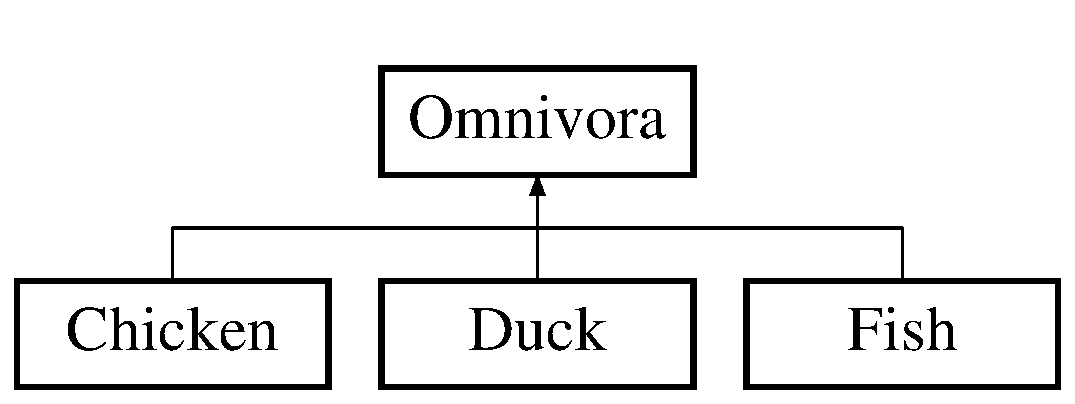
\includegraphics[height=2.000000cm]{classOmnivora}
\end{center}
\end{figure}
\subsection*{Protected Attributes}
\begin{DoxyCompactItemize}
\item 
\hypertarget{classOmnivora_a40a3893e3c10472e89b6d431d38d7cba}{const string {\bfseries tipe\-Makanan} =\char`\"{}omnivora\char`\"{}}\label{classOmnivora_a40a3893e3c10472e89b6d431d38d7cba}

\end{DoxyCompactItemize}


\subsection{Detailed Description}
\hyperlink{classOmnivora}{Omnivora} merupakan tipe \hyperlink{classAnimal}{Animal} pemakan segala 

The documentation for this class was generated from the following file\-:\begin{DoxyCompactItemize}
\item 
Omnivora.\-h\end{DoxyCompactItemize}

\hypertarget{classOwl}{\section{Owl Class Reference}
\label{classOwl}\index{Owl@{Owl}}
}


{\ttfamily \#include $<$Owl.\-h$>$}

Inheritance diagram for Owl\-:\begin{figure}[H]
\begin{center}
\leavevmode
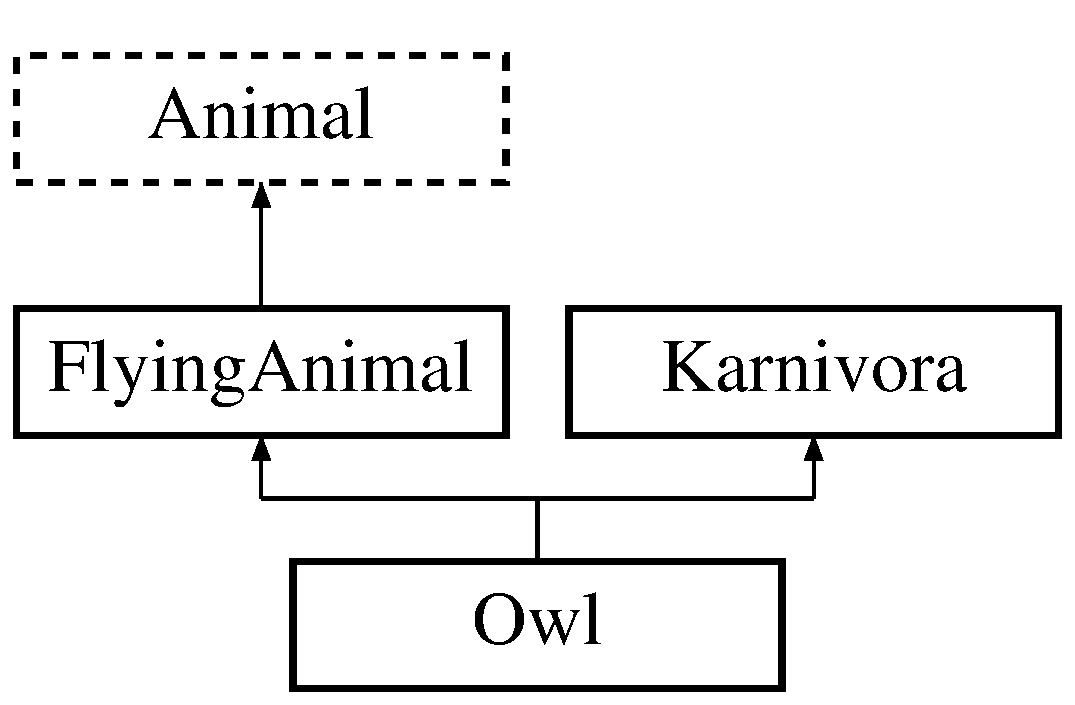
\includegraphics[height=3.000000cm]{classOwl}
\end{center}
\end{figure}
\subsection*{Public Member Functions}
\begin{DoxyCompactItemize}
\item 
\hyperlink{classOwl_a47aecdab1457c845171932653951a1ff}{Owl} (int \-\_\-x, int \-\_\-y)
\begin{DoxyCompactList}\small\item\em Constructor. \end{DoxyCompactList}\item 
\hypertarget{classOwl_af4fdeb54c20c5b9f3ad8aa96bf4324ca}{\hyperlink{classOwl_af4fdeb54c20c5b9f3ad8aa96bf4324ca}{$\sim$\-Owl} ()}\label{classOwl_af4fdeb54c20c5b9f3ad8aa96bf4324ca}

\begin{DoxyCompactList}\small\item\em Destructor. \end{DoxyCompactList}\item 
\hypertarget{classOwl_a168bc318f54f3add5211957d0575aaf2}{void \hyperlink{classOwl_a168bc318f54f3add5211957d0575aaf2}{add\-Bobot} ()}\label{classOwl_a168bc318f54f3add5211957d0575aaf2}

\begin{DoxyCompactList}\small\item\em Menambahkan bobot satu satuan. \end{DoxyCompactList}\item 
int \hyperlink{classOwl_a97186cbd55b070213c8db7274d869a7f}{get\-Bobot} ()
\begin{DoxyCompactList}\small\item\em Mendapatkan nilai bobot dari \hyperlink{classOwl}{Owl}. \end{DoxyCompactList}\item 
char \hyperlink{classOwl_a27ffd4aaac71e68350d53f2f340ef4cb}{get\-Simbol} ()
\begin{DoxyCompactList}\small\item\em Mendapatkan simbol dari \hyperlink{classOwl}{Owl}. \end{DoxyCompactList}\item 
string \hyperlink{classOwl_a670f600b72e5fdb04e11511bd14f63d9}{get\-Musuh} (int i)
\begin{DoxyCompactList}\small\item\em Mendapatkan musuh ke i dari \hyperlink{classOwl}{Owl} Musuh merupakan \hyperlink{classAnimal}{Animal} lain yang tidak bisa tinggal dalam satu kandang dengan \hyperlink{classOwl}{Owl}. \end{DoxyCompactList}\item 
string \hyperlink{classOwl_acc0420063563e1d83d9ae7c3cff311c8}{interact} ()
\begin{DoxyCompactList}\small\item\em Mendapatkan reaksi \hyperlink{classOwl}{Owl} saat berinteraksi dengan pengunjung. \end{DoxyCompactList}\item 
string \hyperlink{classOwl_afbea38ace5450a7bde8caa813adbcfcd}{get\-Tipe\-Animal} ()
\begin{DoxyCompactList}\small\item\em Mendapatkan tipe \hyperlink{classAnimal}{Animal} (nama spesies) \end{DoxyCompactList}\end{DoxyCompactItemize}
\subsection*{Protected Attributes}
\begin{DoxyCompactItemize}
\item 
\hypertarget{classOwl_a1915a017232138322b495efa55e8e1da}{const string {\bfseries tipe\-Animal} = \char`\"{}owl\char`\"{}}\label{classOwl_a1915a017232138322b495efa55e8e1da}

\item 
\hypertarget{classOwl_a069e39ffd838e6e42aa70bac593cd718}{const char {\bfseries simbol} = 'o'}\label{classOwl_a069e39ffd838e6e42aa70bac593cd718}

\item 
\hypertarget{classOwl_ad7a4f92e7f5368ba9dc313b97887bc52}{int {\bfseries bobot}}\label{classOwl_ad7a4f92e7f5368ba9dc313b97887bc52}

\item 
\hypertarget{classOwl_a3924bf902458375d7c97379eadba1554}{string $\ast$ {\bfseries musuh}}\label{classOwl_a3924bf902458375d7c97379eadba1554}

\end{DoxyCompactItemize}


\subsection{Detailed Description}
Merupakan \hyperlink{classAnimal}{Animal} yang tinggal di udara dan merupakan \hyperlink{classKarnivora}{Karnivora} 

\subsection{Constructor \& Destructor Documentation}
\hypertarget{classOwl_a47aecdab1457c845171932653951a1ff}{\index{Owl@{Owl}!Owl@{Owl}}
\index{Owl@{Owl}!Owl@{Owl}}
\subsubsection[{Owl}]{\setlength{\rightskip}{0pt plus 5cm}Owl\-::\-Owl (
\begin{DoxyParamCaption}
\item[{int}]{\-\_\-x, }
\item[{int}]{\-\_\-y}
\end{DoxyParamCaption}
)}}\label{classOwl_a47aecdab1457c845171932653951a1ff}


Constructor. 


\begin{DoxyParams}{Parameters}
{\em \-\_\-x} & posisi x awal \hyperlink{classOwl}{Owl} \\
\hline
{\em \-\_\-y} & posisi y awal \hyperlink{classOwl}{Owl} \\
\hline
\end{DoxyParams}


\subsection{Member Function Documentation}
\hypertarget{classOwl_a97186cbd55b070213c8db7274d869a7f}{\index{Owl@{Owl}!get\-Bobot@{get\-Bobot}}
\index{get\-Bobot@{get\-Bobot}!Owl@{Owl}}
\subsubsection[{get\-Bobot}]{\setlength{\rightskip}{0pt plus 5cm}int Owl\-::get\-Bobot (
\begin{DoxyParamCaption}
{}
\end{DoxyParamCaption}
)\hspace{0.3cm}{\ttfamily [virtual]}}}\label{classOwl_a97186cbd55b070213c8db7274d869a7f}


Mendapatkan nilai bobot dari \hyperlink{classOwl}{Owl}. 

\begin{DoxyReturn}{Returns}
bobot 
\end{DoxyReturn}


Implements \hyperlink{classAnimal}{Animal}.

\hypertarget{classOwl_a670f600b72e5fdb04e11511bd14f63d9}{\index{Owl@{Owl}!get\-Musuh@{get\-Musuh}}
\index{get\-Musuh@{get\-Musuh}!Owl@{Owl}}
\subsubsection[{get\-Musuh}]{\setlength{\rightskip}{0pt plus 5cm}string Owl\-::get\-Musuh (
\begin{DoxyParamCaption}
\item[{int}]{i}
\end{DoxyParamCaption}
)\hspace{0.3cm}{\ttfamily [virtual]}}}\label{classOwl_a670f600b72e5fdb04e11511bd14f63d9}


Mendapatkan musuh ke i dari \hyperlink{classOwl}{Owl} Musuh merupakan \hyperlink{classAnimal}{Animal} lain yang tidak bisa tinggal dalam satu kandang dengan \hyperlink{classOwl}{Owl}. 

\begin{DoxyReturn}{Returns}
musuh\mbox{[}i\mbox{]} 
\end{DoxyReturn}


Implements \hyperlink{classAnimal}{Animal}.

\hypertarget{classOwl_a27ffd4aaac71e68350d53f2f340ef4cb}{\index{Owl@{Owl}!get\-Simbol@{get\-Simbol}}
\index{get\-Simbol@{get\-Simbol}!Owl@{Owl}}
\subsubsection[{get\-Simbol}]{\setlength{\rightskip}{0pt plus 5cm}char Owl\-::get\-Simbol (
\begin{DoxyParamCaption}
{}
\end{DoxyParamCaption}
)\hspace{0.3cm}{\ttfamily [virtual]}}}\label{classOwl_a27ffd4aaac71e68350d53f2f340ef4cb}


Mendapatkan simbol dari \hyperlink{classOwl}{Owl}. 

\begin{DoxyReturn}{Returns}
simbol 
\end{DoxyReturn}


Implements \hyperlink{classAnimal}{Animal}.

\hypertarget{classOwl_afbea38ace5450a7bde8caa813adbcfcd}{\index{Owl@{Owl}!get\-Tipe\-Animal@{get\-Tipe\-Animal}}
\index{get\-Tipe\-Animal@{get\-Tipe\-Animal}!Owl@{Owl}}
\subsubsection[{get\-Tipe\-Animal}]{\setlength{\rightskip}{0pt plus 5cm}string Owl\-::get\-Tipe\-Animal (
\begin{DoxyParamCaption}
{}
\end{DoxyParamCaption}
)\hspace{0.3cm}{\ttfamily [virtual]}}}\label{classOwl_afbea38ace5450a7bde8caa813adbcfcd}


Mendapatkan tipe \hyperlink{classAnimal}{Animal} (nama spesies) 

\begin{DoxyReturn}{Returns}
tipe\-Animal 
\end{DoxyReturn}


Implements \hyperlink{classFlyingAnimal_a1523973b9a6a47e9064825c2134fd65d}{Flying\-Animal}.

\hypertarget{classOwl_acc0420063563e1d83d9ae7c3cff311c8}{\index{Owl@{Owl}!interact@{interact}}
\index{interact@{interact}!Owl@{Owl}}
\subsubsection[{interact}]{\setlength{\rightskip}{0pt plus 5cm}string Owl\-::interact (
\begin{DoxyParamCaption}
{}
\end{DoxyParamCaption}
)\hspace{0.3cm}{\ttfamily [virtual]}}}\label{classOwl_acc0420063563e1d83d9ae7c3cff311c8}


Mendapatkan reaksi \hyperlink{classOwl}{Owl} saat berinteraksi dengan pengunjung. 

\begin{DoxyReturn}{Returns}
\char`\"{}uhukuhuk\char`\"{} 
\end{DoxyReturn}


Implements \hyperlink{classFlyingAnimal_ac0eee625fa2235eee8cbdc0a010ae430}{Flying\-Animal}.



The documentation for this class was generated from the following files\-:\begin{DoxyCompactItemize}
\item 
Owl.\-h\item 
Owl.\-cpp\end{DoxyCompactItemize}

\hypertarget{classPark}{\section{Park Class Reference}
\label{classPark}\index{Park@{Park}}
}


{\ttfamily \#include $<$Park.\-h$>$}

Inheritance diagram for Park\-:\begin{figure}[H]
\begin{center}
\leavevmode
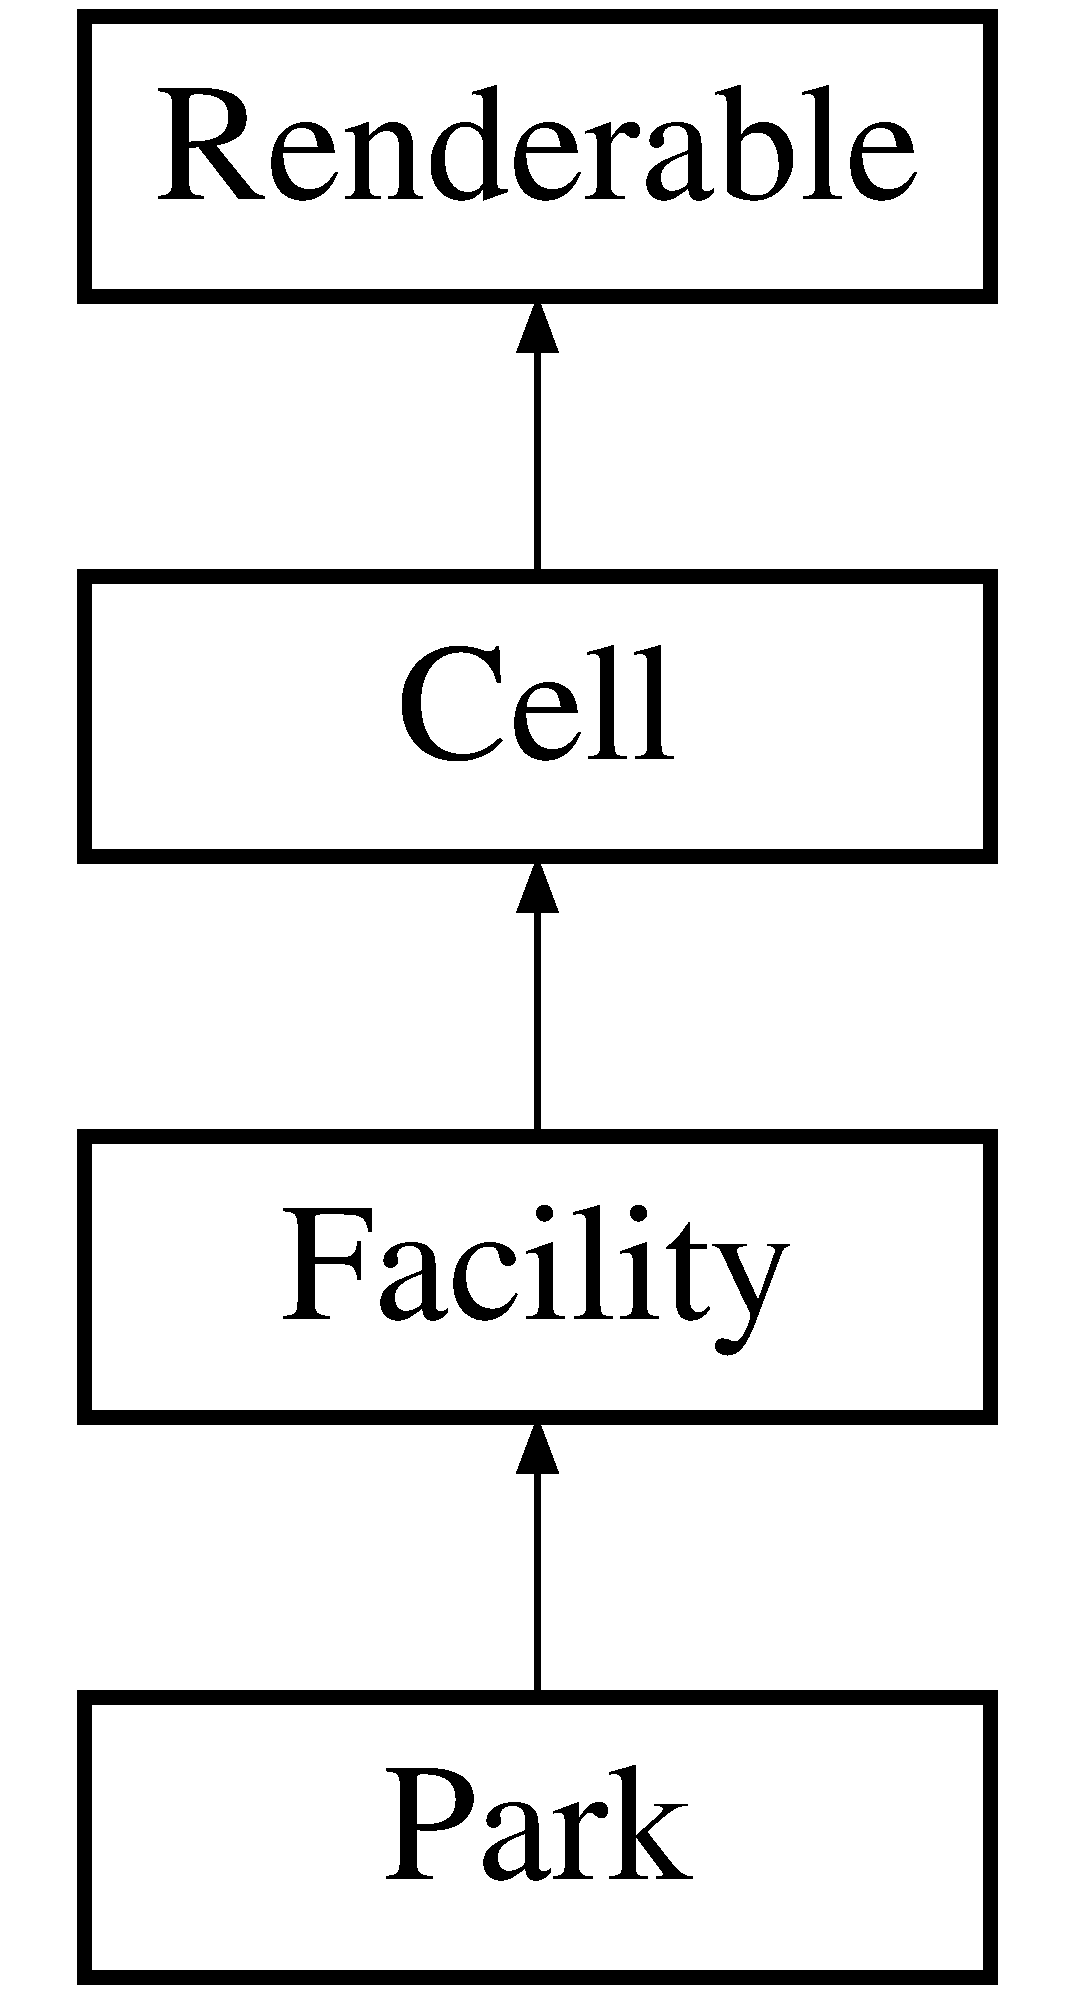
\includegraphics[height=4.000000cm]{classPark}
\end{center}
\end{figure}
\subsection*{Public Member Functions}
\begin{DoxyCompactItemize}
\item 
\hyperlink{classPark_a54fcbf814ca94707bb9c363b6cc32729}{Park} (int x, int y, char s)
\begin{DoxyCompactList}\small\item\em Constructor. \end{DoxyCompactList}\item 
virtual string \hyperlink{classPark_a2b8533d7c9e2024ccc58c57f89f192f2}{get\-Tipe} ()
\begin{DoxyCompactList}\small\item\em Mendapatkan tipe \hyperlink{classCell}{Cell}. \end{DoxyCompactList}\end{DoxyCompactItemize}


\subsection{Detailed Description}
Kelas \hyperlink{classPark}{Park} adalah kelas turunan dari \hyperlink{classFacility}{Facility} 

\subsection{Constructor \& Destructor Documentation}
\hypertarget{classPark_a54fcbf814ca94707bb9c363b6cc32729}{\index{Park@{Park}!Park@{Park}}
\index{Park@{Park}!Park@{Park}}
\subsubsection[{Park}]{\setlength{\rightskip}{0pt plus 5cm}Park\-::\-Park (
\begin{DoxyParamCaption}
\item[{int}]{x, }
\item[{int}]{y, }
\item[{char}]{s}
\end{DoxyParamCaption}
)}}\label{classPark_a54fcbf814ca94707bb9c363b6cc32729}


Constructor. 


\begin{DoxyParams}{Parameters}
{\em x} & Indeks baris \\
\hline
{\em y} & Indeks kolom \\
\hline
{\em s} & Simbol \\
\hline
\end{DoxyParams}


\subsection{Member Function Documentation}
\hypertarget{classPark_a2b8533d7c9e2024ccc58c57f89f192f2}{\index{Park@{Park}!get\-Tipe@{get\-Tipe}}
\index{get\-Tipe@{get\-Tipe}!Park@{Park}}
\subsubsection[{get\-Tipe}]{\setlength{\rightskip}{0pt plus 5cm}string Park\-::get\-Tipe (
\begin{DoxyParamCaption}
{}
\end{DoxyParamCaption}
)\hspace{0.3cm}{\ttfamily [virtual]}}}\label{classPark_a2b8533d7c9e2024ccc58c57f89f192f2}


Mendapatkan tipe \hyperlink{classCell}{Cell}. 

\begin{DoxyReturn}{Returns}
tipe 
\end{DoxyReturn}


Implements \hyperlink{classFacility_a0350c1492460c160c95b1be72ea09860}{Facility}.



The documentation for this class was generated from the following files\-:\begin{DoxyCompactItemize}
\item 
Park.\-h\item 
Park.\-cpp\end{DoxyCompactItemize}

\hypertarget{classRenderable}{\section{Renderable Class Reference}
\label{classRenderable}\index{Renderable@{Renderable}}
}


{\ttfamily \#include $<$Renderable.\-h$>$}

Inheritance diagram for Renderable\-:\begin{figure}[H]
\begin{center}
\leavevmode
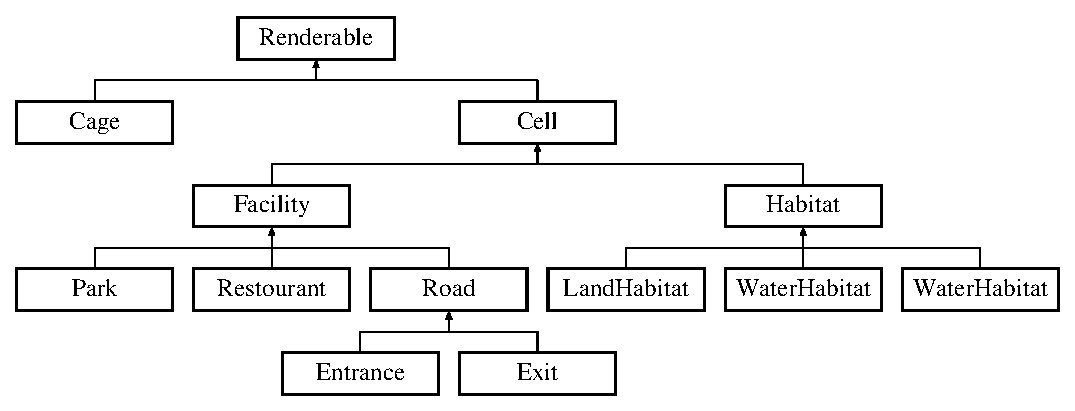
\includegraphics[height=5.000000cm]{classRenderable}
\end{center}
\end{figure}
\subsection*{Public Member Functions}
\begin{DoxyCompactItemize}
\item 
virtual char \hyperlink{classRenderable_aafa9280e6dcfa557b3cd675221fd97b4}{render} ()=0
\end{DoxyCompactItemize}


\subsection{Detailed Description}
Kelas abstrak \hyperlink{classRenderable}{Renderable} merepresentasikan perilaku objek yang dapat digambar di atas layar 

\subsection{Member Function Documentation}
\hypertarget{classRenderable_aafa9280e6dcfa557b3cd675221fd97b4}{\index{Renderable@{Renderable}!render@{render}}
\index{render@{render}!Renderable@{Renderable}}
\subsubsection[{render}]{\setlength{\rightskip}{0pt plus 5cm}virtual char Renderable\-::render (
\begin{DoxyParamCaption}
{}
\end{DoxyParamCaption}
)\hspace{0.3cm}{\ttfamily [pure virtual]}}}\label{classRenderable_aafa9280e6dcfa557b3cd675221fd97b4}
Merupakan method virtual yang mengembalikan satu karakter yang merepresentasikan bentuk objek 

Implemented in \hyperlink{classCage_aab864d541ada79ac83619b139bef5507}{Cage}, and \hyperlink{classCell_a1fc51c6f42b94d1e55f41f068846f523}{Cell}.



The documentation for this class was generated from the following file\-:\begin{DoxyCompactItemize}
\item 
Renderable.\-h\end{DoxyCompactItemize}

\hypertarget{classRestourant}{\section{Restourant Class Reference}
\label{classRestourant}\index{Restourant@{Restourant}}
}


{\ttfamily \#include $<$Restourant.\-h$>$}

Inheritance diagram for Restourant\-:\begin{figure}[H]
\begin{center}
\leavevmode
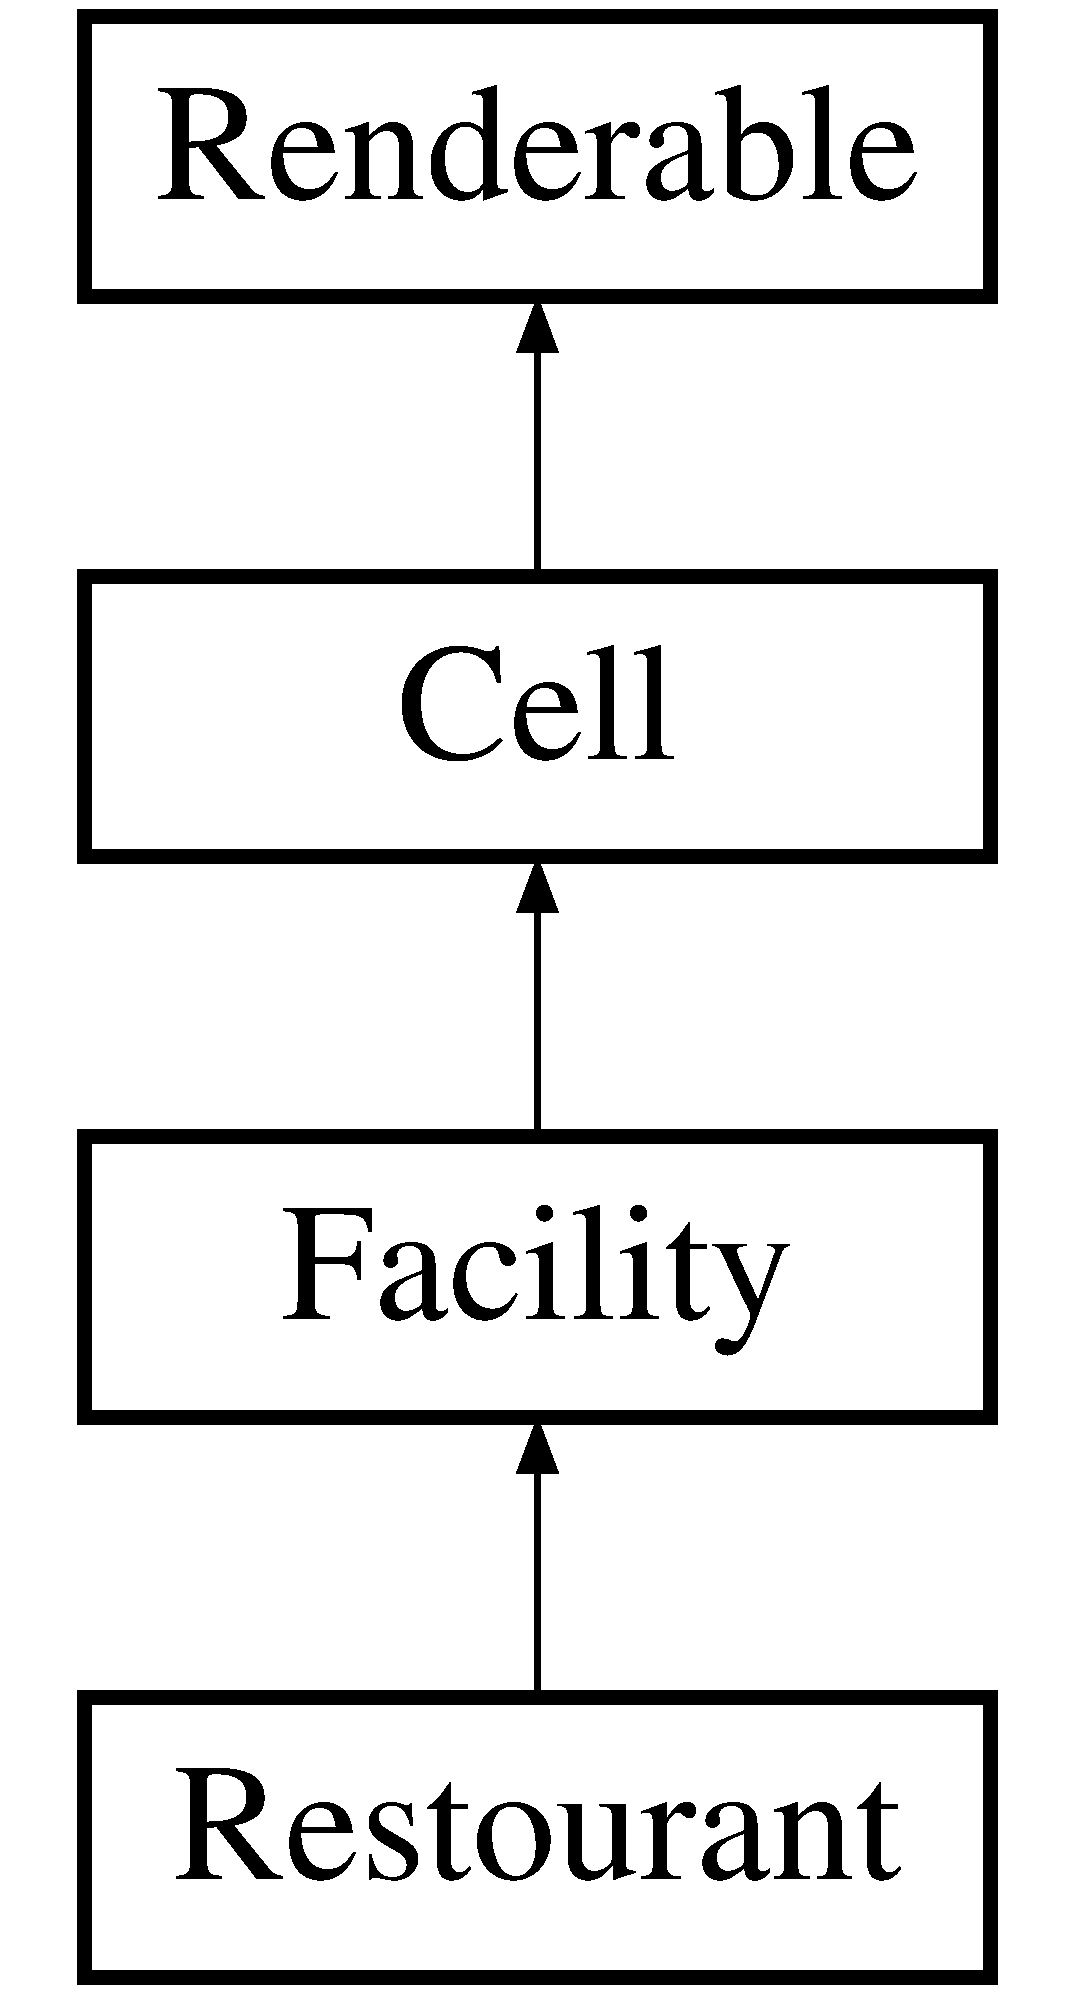
\includegraphics[height=4.000000cm]{classRestourant}
\end{center}
\end{figure}
\subsection*{Public Member Functions}
\begin{DoxyCompactItemize}
\item 
\hyperlink{classRestourant_ad7d9b79b00256cd1ad500459a0fd4883}{Restourant} (int x, int y, char s)
\begin{DoxyCompactList}\small\item\em Constructor. \end{DoxyCompactList}\item 
virtual string \hyperlink{classRestourant_a5f4f9f7229416a7c339bc08c7a50a991}{get\-Tipe} ()
\begin{DoxyCompactList}\small\item\em Mendapatkan tipe \hyperlink{classCell}{Cell}. \end{DoxyCompactList}\end{DoxyCompactItemize}


\subsection{Detailed Description}
Kelas \hyperlink{classRestourant}{Restourant} adalah kelas turunan dari \hyperlink{classFacility}{Facility} 

\subsection{Constructor \& Destructor Documentation}
\hypertarget{classRestourant_ad7d9b79b00256cd1ad500459a0fd4883}{\index{Restourant@{Restourant}!Restourant@{Restourant}}
\index{Restourant@{Restourant}!Restourant@{Restourant}}
\subsubsection[{Restourant}]{\setlength{\rightskip}{0pt plus 5cm}Restourant\-::\-Restourant (
\begin{DoxyParamCaption}
\item[{int}]{x, }
\item[{int}]{y, }
\item[{char}]{s}
\end{DoxyParamCaption}
)}}\label{classRestourant_ad7d9b79b00256cd1ad500459a0fd4883}


Constructor. 


\begin{DoxyParams}{Parameters}
{\em x} & Indeks baris \\
\hline
{\em y} & Indeks kolom \\
\hline
{\em s} & Simbol \\
\hline
\end{DoxyParams}


\subsection{Member Function Documentation}
\hypertarget{classRestourant_a5f4f9f7229416a7c339bc08c7a50a991}{\index{Restourant@{Restourant}!get\-Tipe@{get\-Tipe}}
\index{get\-Tipe@{get\-Tipe}!Restourant@{Restourant}}
\subsubsection[{get\-Tipe}]{\setlength{\rightskip}{0pt plus 5cm}string Restourant\-::get\-Tipe (
\begin{DoxyParamCaption}
{}
\end{DoxyParamCaption}
)\hspace{0.3cm}{\ttfamily [virtual]}}}\label{classRestourant_a5f4f9f7229416a7c339bc08c7a50a991}


Mendapatkan tipe \hyperlink{classCell}{Cell}. 

\begin{DoxyReturn}{Returns}
tipe 
\end{DoxyReturn}


Implements \hyperlink{classFacility_a0350c1492460c160c95b1be72ea09860}{Facility}.



The documentation for this class was generated from the following files\-:\begin{DoxyCompactItemize}
\item 
Restourant.\-h\item 
Restourant.\-cpp\end{DoxyCompactItemize}

\hypertarget{classRhino}{\section{Rhino Class Reference}
\label{classRhino}\index{Rhino@{Rhino}}
}
Inheritance diagram for Rhino\-:\begin{figure}[H]
\begin{center}
\leavevmode
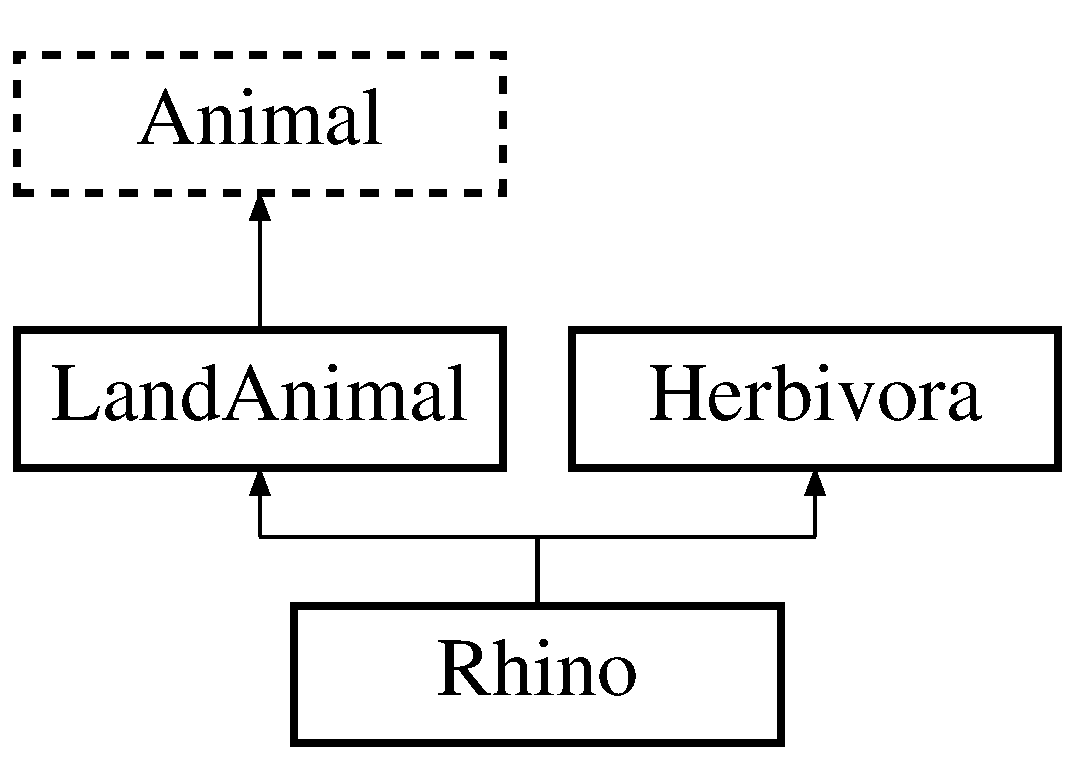
\includegraphics[height=3.000000cm]{classRhino}
\end{center}
\end{figure}
\subsection*{Public Member Functions}
\begin{DoxyCompactItemize}
\item 
\hyperlink{classRhino_a58522b211956561033d02c692f8efbf0}{Rhino} (int \-\_\-x, int \-\_\-y)
\begin{DoxyCompactList}\small\item\em Constructor. \end{DoxyCompactList}\item 
\hypertarget{classRhino_a6a11f0f8dcd6ed20ef99d8d698b06f28}{\hyperlink{classRhino_a6a11f0f8dcd6ed20ef99d8d698b06f28}{$\sim$\-Rhino} ()}\label{classRhino_a6a11f0f8dcd6ed20ef99d8d698b06f28}

\begin{DoxyCompactList}\small\item\em Destructor. \end{DoxyCompactList}\item 
\hypertarget{classRhino_a83ba6ae8becb9c7aa8f7e17b9783085b}{void \hyperlink{classRhino_a83ba6ae8becb9c7aa8f7e17b9783085b}{add\-Bobot} ()}\label{classRhino_a83ba6ae8becb9c7aa8f7e17b9783085b}

\begin{DoxyCompactList}\small\item\em Menambahkan bobot satu satuan. \end{DoxyCompactList}\item 
int \hyperlink{classRhino_a624cabcc67d0be3ccdb21c8bf63a3ccd}{get\-Bobot} ()
\begin{DoxyCompactList}\small\item\em Mendapatkan nilai bobot dari \hyperlink{classSnake}{Snake}. \end{DoxyCompactList}\item 
char \hyperlink{classRhino_ad686dce9238ac3e5baaaa205cc07ddb9}{get\-Simbol} ()
\begin{DoxyCompactList}\small\item\em Mendapatkan simbol dari \hyperlink{classSnake}{Snake}. \end{DoxyCompactList}\item 
string \hyperlink{classRhino_a52916d0a7fd7a97ae11571e2c9511d5f}{get\-Musuh} (int i)
\begin{DoxyCompactList}\small\item\em Mendapatkan musuh ke i dari \hyperlink{classSnake}{Snake} Musuh merupakan \hyperlink{classAnimal}{Animal} lain yang tidak bisa tinggal dalam satu kandang dengan \hyperlink{classSnake}{Snake}. \end{DoxyCompactList}\item 
string \hyperlink{classRhino_ab58c391c33619b17b06f39f919b4737c}{interact} ()
\begin{DoxyCompactList}\small\item\em Mendapatkan reaksi \hyperlink{classSnake}{Snake} saat berinteraksi dengan pengunjung. \end{DoxyCompactList}\item 
string \hyperlink{classRhino_ab1a961793213c332a9a23180c7700bc7}{get\-Tipe\-Animal} ()
\begin{DoxyCompactList}\small\item\em Mendapatkan tipe \hyperlink{classAnimal}{Animal} (nama spesies) \end{DoxyCompactList}\end{DoxyCompactItemize}
\subsection*{Protected Attributes}
\begin{DoxyCompactItemize}
\item 
\hypertarget{classRhino_aaf8af4721ce0a164afb6328ee61d4bb1}{const string {\bfseries tipe\-Animal} = \char`\"{}rhino\char`\"{}}\label{classRhino_aaf8af4721ce0a164afb6328ee61d4bb1}

\item 
\hypertarget{classRhino_aa4a322a2e0e81ecc6a3048bdb262b22c}{const char {\bfseries simbol} = 'r'}\label{classRhino_aa4a322a2e0e81ecc6a3048bdb262b22c}

\item 
\hypertarget{classRhino_a61bfc712bed65dea8effae1d330c98a3}{int {\bfseries bobot}}\label{classRhino_a61bfc712bed65dea8effae1d330c98a3}

\item 
\hypertarget{classRhino_aa3af85ef27fed2d5ebce1a2113366ecd}{string $\ast$ {\bfseries musuh}}\label{classRhino_aa3af85ef27fed2d5ebce1a2113366ecd}

\end{DoxyCompactItemize}


\subsection{Constructor \& Destructor Documentation}
\hypertarget{classRhino_a58522b211956561033d02c692f8efbf0}{\index{Rhino@{Rhino}!Rhino@{Rhino}}
\index{Rhino@{Rhino}!Rhino@{Rhino}}
\subsubsection[{Rhino}]{\setlength{\rightskip}{0pt plus 5cm}Rhino\-::\-Rhino (
\begin{DoxyParamCaption}
\item[{int}]{\-\_\-x, }
\item[{int}]{\-\_\-y}
\end{DoxyParamCaption}
)}}\label{classRhino_a58522b211956561033d02c692f8efbf0}


Constructor. 


\begin{DoxyParams}{Parameters}
{\em \-\_\-x} & posisi x awal \hyperlink{classSnake}{Snake} \\
\hline
{\em \-\_\-y} & posisi y awal \hyperlink{classSnake}{Snake} \\
\hline
\end{DoxyParams}


\subsection{Member Function Documentation}
\hypertarget{classRhino_a624cabcc67d0be3ccdb21c8bf63a3ccd}{\index{Rhino@{Rhino}!get\-Bobot@{get\-Bobot}}
\index{get\-Bobot@{get\-Bobot}!Rhino@{Rhino}}
\subsubsection[{get\-Bobot}]{\setlength{\rightskip}{0pt plus 5cm}int Rhino\-::get\-Bobot (
\begin{DoxyParamCaption}
{}
\end{DoxyParamCaption}
)\hspace{0.3cm}{\ttfamily [virtual]}}}\label{classRhino_a624cabcc67d0be3ccdb21c8bf63a3ccd}


Mendapatkan nilai bobot dari \hyperlink{classSnake}{Snake}. 

\begin{DoxyReturn}{Returns}
bobot 
\end{DoxyReturn}


Implements \hyperlink{classAnimal}{Animal}.

\hypertarget{classRhino_a52916d0a7fd7a97ae11571e2c9511d5f}{\index{Rhino@{Rhino}!get\-Musuh@{get\-Musuh}}
\index{get\-Musuh@{get\-Musuh}!Rhino@{Rhino}}
\subsubsection[{get\-Musuh}]{\setlength{\rightskip}{0pt plus 5cm}string Rhino\-::get\-Musuh (
\begin{DoxyParamCaption}
\item[{int}]{i}
\end{DoxyParamCaption}
)\hspace{0.3cm}{\ttfamily [virtual]}}}\label{classRhino_a52916d0a7fd7a97ae11571e2c9511d5f}


Mendapatkan musuh ke i dari \hyperlink{classSnake}{Snake} Musuh merupakan \hyperlink{classAnimal}{Animal} lain yang tidak bisa tinggal dalam satu kandang dengan \hyperlink{classSnake}{Snake}. 

\begin{DoxyReturn}{Returns}
musuh\mbox{[}i\mbox{]} 
\end{DoxyReturn}


Implements \hyperlink{classAnimal}{Animal}.

\hypertarget{classRhino_ad686dce9238ac3e5baaaa205cc07ddb9}{\index{Rhino@{Rhino}!get\-Simbol@{get\-Simbol}}
\index{get\-Simbol@{get\-Simbol}!Rhino@{Rhino}}
\subsubsection[{get\-Simbol}]{\setlength{\rightskip}{0pt plus 5cm}char Rhino\-::get\-Simbol (
\begin{DoxyParamCaption}
{}
\end{DoxyParamCaption}
)\hspace{0.3cm}{\ttfamily [virtual]}}}\label{classRhino_ad686dce9238ac3e5baaaa205cc07ddb9}


Mendapatkan simbol dari \hyperlink{classSnake}{Snake}. 

\begin{DoxyReturn}{Returns}
simbol 
\end{DoxyReturn}


Implements \hyperlink{classAnimal}{Animal}.

\hypertarget{classRhino_ab1a961793213c332a9a23180c7700bc7}{\index{Rhino@{Rhino}!get\-Tipe\-Animal@{get\-Tipe\-Animal}}
\index{get\-Tipe\-Animal@{get\-Tipe\-Animal}!Rhino@{Rhino}}
\subsubsection[{get\-Tipe\-Animal}]{\setlength{\rightskip}{0pt plus 5cm}string Rhino\-::get\-Tipe\-Animal (
\begin{DoxyParamCaption}
{}
\end{DoxyParamCaption}
)\hspace{0.3cm}{\ttfamily [virtual]}}}\label{classRhino_ab1a961793213c332a9a23180c7700bc7}


Mendapatkan tipe \hyperlink{classAnimal}{Animal} (nama spesies) 

\begin{DoxyReturn}{Returns}
tipe\-Animal 
\end{DoxyReturn}


Implements \hyperlink{classLandAnimal}{Land\-Animal}.

\hypertarget{classRhino_ab58c391c33619b17b06f39f919b4737c}{\index{Rhino@{Rhino}!interact@{interact}}
\index{interact@{interact}!Rhino@{Rhino}}
\subsubsection[{interact}]{\setlength{\rightskip}{0pt plus 5cm}string Rhino\-::interact (
\begin{DoxyParamCaption}
{}
\end{DoxyParamCaption}
)\hspace{0.3cm}{\ttfamily [virtual]}}}\label{classRhino_ab58c391c33619b17b06f39f919b4737c}


Mendapatkan reaksi \hyperlink{classSnake}{Snake} saat berinteraksi dengan pengunjung. 

\begin{DoxyReturn}{Returns}
\char`\"{}culacula\char`\"{} 
\end{DoxyReturn}


Implements \hyperlink{classLandAnimal}{Land\-Animal}.



The documentation for this class was generated from the following files\-:\begin{DoxyCompactItemize}
\item 
Rhino.\-h\item 
Rhino.\-cpp\end{DoxyCompactItemize}

\hypertarget{classRoad}{\section{Road Class Reference}
\label{classRoad}\index{Road@{Road}}
}
Inheritance diagram for Road\-:\begin{figure}[H]
\begin{center}
\leavevmode
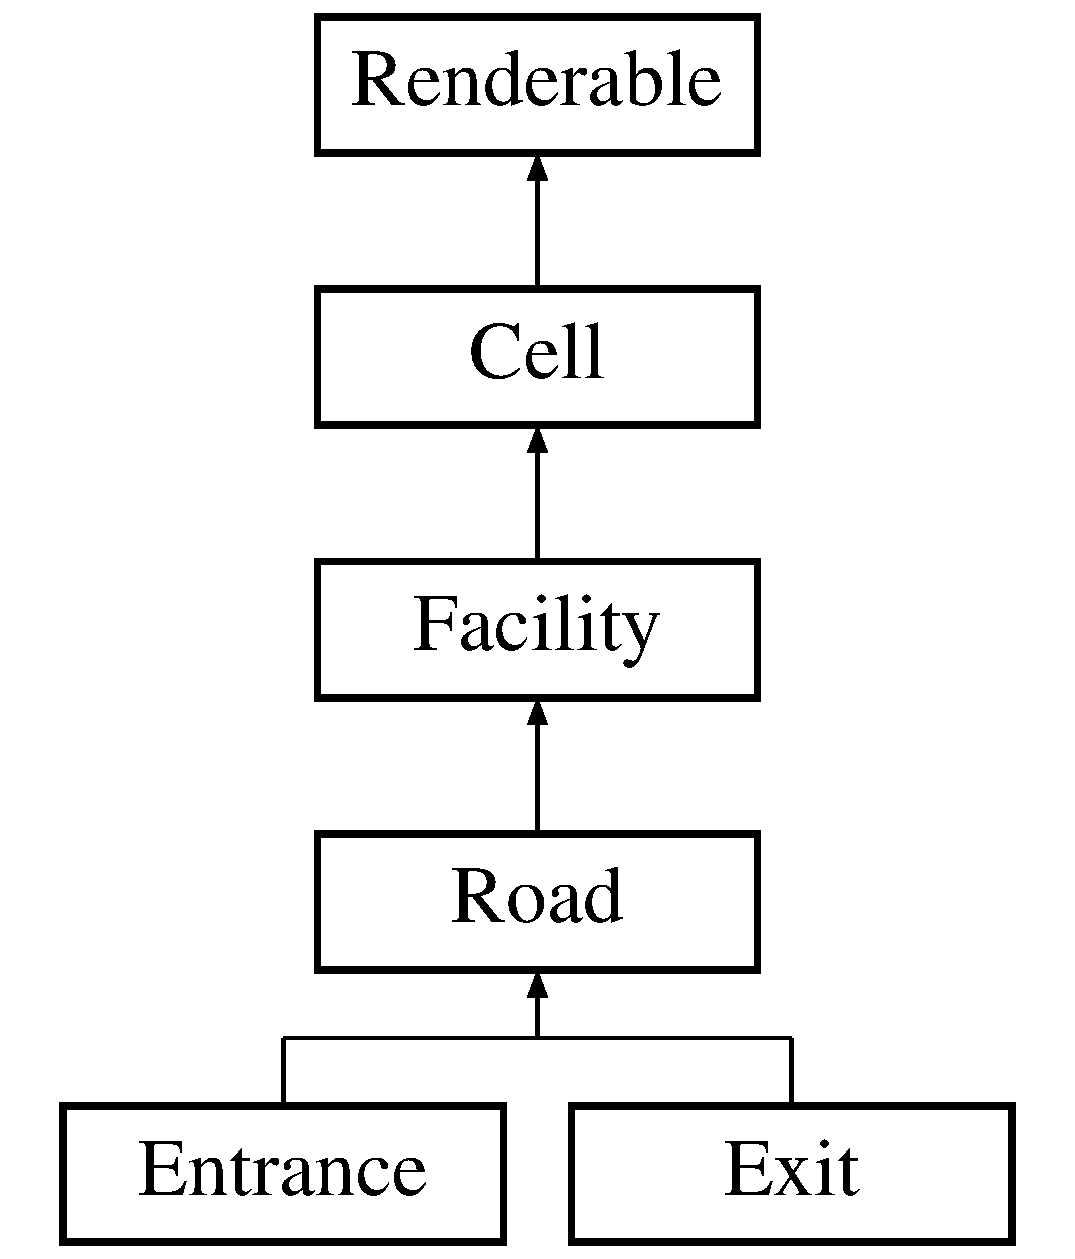
\includegraphics[height=5.000000cm]{classRoad}
\end{center}
\end{figure}
\subsection*{Public Member Functions}
\begin{DoxyCompactItemize}
\item 
\hyperlink{classRoad_adcd58beb66dbf9a54ab5200bab41d6f6}{Road} (int x, int y, char s)
\begin{DoxyCompactList}\small\item\em Constructor. \end{DoxyCompactList}\item 
virtual string \hyperlink{classRoad_a750f8b4ab694ed29e8bd6db4d9758429}{get\-Tipe} ()
\begin{DoxyCompactList}\small\item\em Mendapatkan tipe \hyperlink{classCell}{Cell}. \end{DoxyCompactList}\end{DoxyCompactItemize}


\subsection{Constructor \& Destructor Documentation}
\hypertarget{classRoad_adcd58beb66dbf9a54ab5200bab41d6f6}{\index{Road@{Road}!Road@{Road}}
\index{Road@{Road}!Road@{Road}}
\subsubsection[{Road}]{\setlength{\rightskip}{0pt plus 5cm}Road\-::\-Road (
\begin{DoxyParamCaption}
\item[{int}]{x, }
\item[{int}]{y, }
\item[{char}]{s}
\end{DoxyParamCaption}
)}}\label{classRoad_adcd58beb66dbf9a54ab5200bab41d6f6}


Constructor. 


\begin{DoxyParams}{Parameters}
{\em x} & Indeks baris \\
\hline
{\em y} & Indeks kolom \\
\hline
{\em s} & Simbol \\
\hline
\end{DoxyParams}


\subsection{Member Function Documentation}
\hypertarget{classRoad_a750f8b4ab694ed29e8bd6db4d9758429}{\index{Road@{Road}!get\-Tipe@{get\-Tipe}}
\index{get\-Tipe@{get\-Tipe}!Road@{Road}}
\subsubsection[{get\-Tipe}]{\setlength{\rightskip}{0pt plus 5cm}string Road\-::get\-Tipe (
\begin{DoxyParamCaption}
{}
\end{DoxyParamCaption}
)\hspace{0.3cm}{\ttfamily [virtual]}}}\label{classRoad_a750f8b4ab694ed29e8bd6db4d9758429}


Mendapatkan tipe \hyperlink{classCell}{Cell}. 

\begin{DoxyReturn}{Returns}
tipe 
\end{DoxyReturn}


Implements \hyperlink{classFacility_a0350c1492460c160c95b1be72ea09860}{Facility}.



Reimplemented in \hyperlink{classEntrance_afff61031d269e47536b3bf4821ab0dda}{Entrance}, and \hyperlink{classExit_aa769d720f40b684da6ca21fc2515f910}{Exit}.



The documentation for this class was generated from the following files\-:\begin{DoxyCompactItemize}
\item 
Road.\-h\item 
Road.\-cpp\end{DoxyCompactItemize}

\hypertarget{classSnake}{\section{Snake Class Reference}
\label{classSnake}\index{Snake@{Snake}}
}


{\ttfamily \#include $<$Elephant.\-h$>$}

Inheritance diagram for Snake\-:\begin{figure}[H]
\begin{center}
\leavevmode
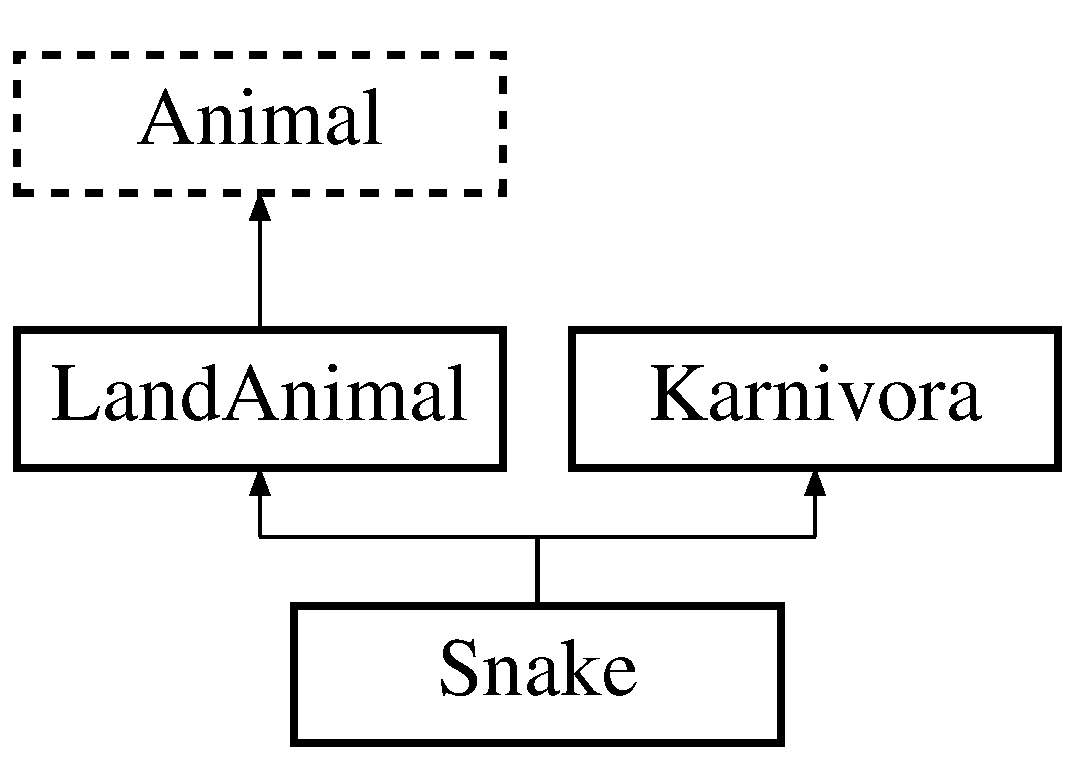
\includegraphics[height=3.000000cm]{classSnake}
\end{center}
\end{figure}
\subsection*{Public Member Functions}
\begin{DoxyCompactItemize}
\item 
\hyperlink{classSnake_a94d42d8a098d807f5ab45d1074269b08}{Snake} (int \-\_\-x, int \-\_\-y)
\begin{DoxyCompactList}\small\item\em Constructor. \end{DoxyCompactList}\item 
\hypertarget{classSnake_a941fbaad96ee33ca3a7c30c28ca44ef8}{\hyperlink{classSnake_a941fbaad96ee33ca3a7c30c28ca44ef8}{$\sim$\-Snake} ()}\label{classSnake_a941fbaad96ee33ca3a7c30c28ca44ef8}

\begin{DoxyCompactList}\small\item\em Destructor. \end{DoxyCompactList}\item 
\hypertarget{classSnake_a145debb3583b794ea74a26fa0b94b542}{void \hyperlink{classSnake_a145debb3583b794ea74a26fa0b94b542}{add\-Bobot} ()}\label{classSnake_a145debb3583b794ea74a26fa0b94b542}

\begin{DoxyCompactList}\small\item\em Menambahkan bobot satu satuan. \end{DoxyCompactList}\item 
int \hyperlink{classSnake_a116efbdf57f0a8136a1d6ab794e5954b}{get\-Bobot} ()
\begin{DoxyCompactList}\small\item\em Mendapatkan nilai bobot dari \hyperlink{classSnake}{Snake}. \end{DoxyCompactList}\item 
char \hyperlink{classSnake_a5801f234eba23051115dddcdfa29aa72}{get\-Simbol} ()
\begin{DoxyCompactList}\small\item\em Mendapatkan simbol dari \hyperlink{classSnake}{Snake}. \end{DoxyCompactList}\item 
string \hyperlink{classSnake_ae1008e9565a5cb58ec355a67d68341bb}{get\-Musuh} (int i)
\begin{DoxyCompactList}\small\item\em Mendapatkan musuh ke i dari \hyperlink{classSnake}{Snake} Musuh merupakan \hyperlink{classAnimal}{Animal} lain yang tidak bisa tinggal dalam satu kandang dengan \hyperlink{classSnake}{Snake}. \end{DoxyCompactList}\item 
string \hyperlink{classSnake_a974f553600bb0984b2fa502ec5be3855}{interact} ()
\begin{DoxyCompactList}\small\item\em Mendapatkan reaksi \hyperlink{classSnake}{Snake} saat berinteraksi dengan pengunjung. \end{DoxyCompactList}\item 
string \hyperlink{classSnake_a54fc47d99473a45311841d3a6f436139}{get\-Tipe\-Animal} ()
\begin{DoxyCompactList}\small\item\em Mendapatkan tipe \hyperlink{classAnimal}{Animal} (nama spesies) \end{DoxyCompactList}\end{DoxyCompactItemize}
\subsection*{Protected Attributes}
\begin{DoxyCompactItemize}
\item 
\hypertarget{classSnake_a55432acef37a555755f640d46220a0db}{const string {\bfseries tipe\-Animal} = \char`\"{}snake\char`\"{}}\label{classSnake_a55432acef37a555755f640d46220a0db}

\item 
\hypertarget{classSnake_a16b8be93c26ea8697c3d0ef20aef4dd1}{const char {\bfseries simbol} = 's'}\label{classSnake_a16b8be93c26ea8697c3d0ef20aef4dd1}

\item 
\hypertarget{classSnake_af825855d802658c24b0702103acb84c6}{int {\bfseries bobot}}\label{classSnake_af825855d802658c24b0702103acb84c6}

\item 
\hypertarget{classSnake_aacdf64a9824a0e2e3143143dbc1adb77}{string $\ast$ {\bfseries musuh}}\label{classSnake_aacdf64a9824a0e2e3143143dbc1adb77}

\end{DoxyCompactItemize}


\subsection{Detailed Description}
Merupakan \hyperlink{classAnimal}{Animal} yang tinggal di darat dan merupakan \hyperlink{classHerbivora}{Herbivora}

Merupakan \hyperlink{classAnimal}{Animal} yang tinggal di darat dan merupakan \hyperlink{classKarnivora}{Karnivora} 

\subsection{Constructor \& Destructor Documentation}
\hypertarget{classSnake_a94d42d8a098d807f5ab45d1074269b08}{\index{Snake@{Snake}!Snake@{Snake}}
\index{Snake@{Snake}!Snake@{Snake}}
\subsubsection[{Snake}]{\setlength{\rightskip}{0pt plus 5cm}Snake\-::\-Snake (
\begin{DoxyParamCaption}
\item[{int}]{\-\_\-x, }
\item[{int}]{\-\_\-y}
\end{DoxyParamCaption}
)}}\label{classSnake_a94d42d8a098d807f5ab45d1074269b08}


Constructor. 


\begin{DoxyParams}{Parameters}
{\em \-\_\-x} & posisi x awal \hyperlink{classSnake}{Snake} \\
\hline
{\em \-\_\-y} & posisi y awal \hyperlink{classSnake}{Snake} \\
\hline
\end{DoxyParams}


\subsection{Member Function Documentation}
\hypertarget{classSnake_a116efbdf57f0a8136a1d6ab794e5954b}{\index{Snake@{Snake}!get\-Bobot@{get\-Bobot}}
\index{get\-Bobot@{get\-Bobot}!Snake@{Snake}}
\subsubsection[{get\-Bobot}]{\setlength{\rightskip}{0pt plus 5cm}int Snake\-::get\-Bobot (
\begin{DoxyParamCaption}
{}
\end{DoxyParamCaption}
)\hspace{0.3cm}{\ttfamily [virtual]}}}\label{classSnake_a116efbdf57f0a8136a1d6ab794e5954b}


Mendapatkan nilai bobot dari \hyperlink{classSnake}{Snake}. 

\begin{DoxyReturn}{Returns}
bobot 
\end{DoxyReturn}


Implements \hyperlink{classAnimal}{Animal}.

\hypertarget{classSnake_ae1008e9565a5cb58ec355a67d68341bb}{\index{Snake@{Snake}!get\-Musuh@{get\-Musuh}}
\index{get\-Musuh@{get\-Musuh}!Snake@{Snake}}
\subsubsection[{get\-Musuh}]{\setlength{\rightskip}{0pt plus 5cm}string Snake\-::get\-Musuh (
\begin{DoxyParamCaption}
\item[{int}]{i}
\end{DoxyParamCaption}
)\hspace{0.3cm}{\ttfamily [virtual]}}}\label{classSnake_ae1008e9565a5cb58ec355a67d68341bb}


Mendapatkan musuh ke i dari \hyperlink{classSnake}{Snake} Musuh merupakan \hyperlink{classAnimal}{Animal} lain yang tidak bisa tinggal dalam satu kandang dengan \hyperlink{classSnake}{Snake}. 

\begin{DoxyReturn}{Returns}
musuh\mbox{[}i\mbox{]} 
\end{DoxyReturn}


Implements \hyperlink{classAnimal}{Animal}.

\hypertarget{classSnake_a5801f234eba23051115dddcdfa29aa72}{\index{Snake@{Snake}!get\-Simbol@{get\-Simbol}}
\index{get\-Simbol@{get\-Simbol}!Snake@{Snake}}
\subsubsection[{get\-Simbol}]{\setlength{\rightskip}{0pt plus 5cm}char Snake\-::get\-Simbol (
\begin{DoxyParamCaption}
{}
\end{DoxyParamCaption}
)\hspace{0.3cm}{\ttfamily [virtual]}}}\label{classSnake_a5801f234eba23051115dddcdfa29aa72}


Mendapatkan simbol dari \hyperlink{classSnake}{Snake}. 

\begin{DoxyReturn}{Returns}
simbol 
\end{DoxyReturn}


Implements \hyperlink{classAnimal}{Animal}.

\hypertarget{classSnake_a54fc47d99473a45311841d3a6f436139}{\index{Snake@{Snake}!get\-Tipe\-Animal@{get\-Tipe\-Animal}}
\index{get\-Tipe\-Animal@{get\-Tipe\-Animal}!Snake@{Snake}}
\subsubsection[{get\-Tipe\-Animal}]{\setlength{\rightskip}{0pt plus 5cm}string Snake\-::get\-Tipe\-Animal (
\begin{DoxyParamCaption}
{}
\end{DoxyParamCaption}
)\hspace{0.3cm}{\ttfamily [virtual]}}}\label{classSnake_a54fc47d99473a45311841d3a6f436139}


Mendapatkan tipe \hyperlink{classAnimal}{Animal} (nama spesies) 

\begin{DoxyReturn}{Returns}
tipe\-Animal 
\end{DoxyReturn}


Implements \hyperlink{classLandAnimal}{Land\-Animal}.

\hypertarget{classSnake_a974f553600bb0984b2fa502ec5be3855}{\index{Snake@{Snake}!interact@{interact}}
\index{interact@{interact}!Snake@{Snake}}
\subsubsection[{interact}]{\setlength{\rightskip}{0pt plus 5cm}string Snake\-::interact (
\begin{DoxyParamCaption}
{}
\end{DoxyParamCaption}
)\hspace{0.3cm}{\ttfamily [virtual]}}}\label{classSnake_a974f553600bb0984b2fa502ec5be3855}


Mendapatkan reaksi \hyperlink{classSnake}{Snake} saat berinteraksi dengan pengunjung. 

\begin{DoxyReturn}{Returns}
\char`\"{}ssstt\char`\"{} 
\end{DoxyReturn}


Implements \hyperlink{classLandAnimal}{Land\-Animal}.



The documentation for this class was generated from the following files\-:\begin{DoxyCompactItemize}
\item 
Snake.\-h\item 
Snake.\-cpp\end{DoxyCompactItemize}

\hypertarget{classView}{\section{View Class Reference}
\label{classView}\index{View@{View}}
}


{\ttfamily \#include $<$View.\-h$>$}

\subsection*{Public Member Functions}
\begin{DoxyCompactItemize}
\item 
\hyperlink{classView_aac96eba98e7f531e94ad15a892e19dbd}{View} (int len, int wid)
\begin{DoxyCompactList}\small\item\em Constructor. \end{DoxyCompactList}\item 
\hypertarget{classView_aa373ca7c069a854e1e8821b0f13aa186}{\hyperlink{classView_aa373ca7c069a854e1e8821b0f13aa186}{View} (const \hyperlink{classView}{View} \&)}\label{classView_aa373ca7c069a854e1e8821b0f13aa186}

\begin{DoxyCompactList}\small\item\em Copy Constructor. \end{DoxyCompactList}\item 
\hypertarget{classView_ad0dc854db9aabbea98a334dec89f785c}{\hyperlink{classView_ad0dc854db9aabbea98a334dec89f785c}{$\sim$\-View} ()}\label{classView_ad0dc854db9aabbea98a334dec89f785c}

\begin{DoxyCompactList}\small\item\em Destructor. \end{DoxyCompactList}\item 
char \hyperlink{classView_aa6bd990eaac4d2991f27b304213b54ef}{get\-Val} (int \-\_\-x, int \-\_\-y)
\begin{DoxyCompactList}\small\item\em Mendapatkan nilai val\mbox{[}\-\_\-x\mbox{]}\mbox{[}\-\_\-y\mbox{]}. \end{DoxyCompactList}\item 
void \hyperlink{classView_a21cba84b1b3374baaec030a21128db47}{set\-Val} (int i, int j, char c)
\begin{DoxyCompactList}\small\item\em Mengubah nilai val\mbox{[}i\mbox{]}\mbox{[}j\mbox{]} menjadi c. \end{DoxyCompactList}\item 
int \hyperlink{classView_a62ae4de313b6643810b989ae988a1640}{get\-N\-B\-R\-S} ()
\begin{DoxyCompactList}\small\item\em Mendapatkan nilai baris. \end{DoxyCompactList}\item 
int \hyperlink{classView_a03b9f87a6e0aada6ddabaa459e261848}{get\-N\-K\-O\-L} ()
\begin{DoxyCompactList}\small\item\em Mendapatkan nilai kolom. \end{DoxyCompactList}\item 
\hypertarget{classView_a769e75520faca6d5bd21d8e4905d4341}{void \hyperlink{classView_a769e75520faca6d5bd21d8e4905d4341}{print\-View} ()}\label{classView_a769e75520faca6d5bd21d8e4905d4341}

\begin{DoxyCompactList}\small\item\em Mencetak seluruh karakter yang ada. \end{DoxyCompactList}\item 
\hypertarget{classView_a228842cd6673f8f436e00bf5f5f649fe}{void \hyperlink{classView_a228842cd6673f8f436e00bf5f5f649fe}{print\-View} (int kiri, int atas, int kanan, int bawah)}\label{classView_a228842cd6673f8f436e00bf5f5f649fe}

\begin{DoxyCompactList}\small\item\em Mencetak karakter pada area mulai dari titik kiri atas sampai kanan bawah. \end{DoxyCompactList}\end{DoxyCompactItemize}


\subsection{Detailed Description}
Kelas \hyperlink{classView}{View} merupakan container dalam bentuk matriks dari karakter2 yang nantinya akan dicetak ke layar 

\subsection{Constructor \& Destructor Documentation}
\hypertarget{classView_aac96eba98e7f531e94ad15a892e19dbd}{\index{View@{View}!View@{View}}
\index{View@{View}!View@{View}}
\subsubsection[{View}]{\setlength{\rightskip}{0pt plus 5cm}View\-::\-View (
\begin{DoxyParamCaption}
\item[{int}]{len, }
\item[{int}]{wid}
\end{DoxyParamCaption}
)}}\label{classView_aac96eba98e7f531e94ad15a892e19dbd}


Constructor. 


\begin{DoxyParams}{Parameters}
{\em len} & Nilai N\-B\-R\-S \\
\hline
{\em wid} & Nilai N\-K\-O\-L \\
\hline
\end{DoxyParams}


\subsection{Member Function Documentation}
\hypertarget{classView_a62ae4de313b6643810b989ae988a1640}{\index{View@{View}!get\-N\-B\-R\-S@{get\-N\-B\-R\-S}}
\index{get\-N\-B\-R\-S@{get\-N\-B\-R\-S}!View@{View}}
\subsubsection[{get\-N\-B\-R\-S}]{\setlength{\rightskip}{0pt plus 5cm}int View\-::get\-N\-B\-R\-S (
\begin{DoxyParamCaption}
{}
\end{DoxyParamCaption}
)}}\label{classView_a62ae4de313b6643810b989ae988a1640}


Mendapatkan nilai baris. 

\begin{DoxyReturn}{Returns}
N\-B\-R\-S 
\end{DoxyReturn}
\hypertarget{classView_a03b9f87a6e0aada6ddabaa459e261848}{\index{View@{View}!get\-N\-K\-O\-L@{get\-N\-K\-O\-L}}
\index{get\-N\-K\-O\-L@{get\-N\-K\-O\-L}!View@{View}}
\subsubsection[{get\-N\-K\-O\-L}]{\setlength{\rightskip}{0pt plus 5cm}int View\-::get\-N\-K\-O\-L (
\begin{DoxyParamCaption}
{}
\end{DoxyParamCaption}
)}}\label{classView_a03b9f87a6e0aada6ddabaa459e261848}


Mendapatkan nilai kolom. 

\begin{DoxyReturn}{Returns}
N\-K\-O\-L 
\end{DoxyReturn}
\hypertarget{classView_aa6bd990eaac4d2991f27b304213b54ef}{\index{View@{View}!get\-Val@{get\-Val}}
\index{get\-Val@{get\-Val}!View@{View}}
\subsubsection[{get\-Val}]{\setlength{\rightskip}{0pt plus 5cm}char View\-::get\-Val (
\begin{DoxyParamCaption}
\item[{int}]{\-\_\-x, }
\item[{int}]{\-\_\-y}
\end{DoxyParamCaption}
)}}\label{classView_aa6bd990eaac4d2991f27b304213b54ef}


Mendapatkan nilai val\mbox{[}\-\_\-x\mbox{]}\mbox{[}\-\_\-y\mbox{]}. 


\begin{DoxyParams}{Parameters}
{\em \-\_\-x} & Index baris nilai yang ingin didapatkan \\
\hline
{\em \-\_\-y} & Index kolom nilai yang ingin didapatkan \\
\hline
\end{DoxyParams}
\begin{DoxyReturn}{Returns}
val\mbox{[}\-\_\-x\mbox{]}\mbox{[}\-\_\-y\mbox{]} 
\end{DoxyReturn}
\hypertarget{classView_a21cba84b1b3374baaec030a21128db47}{\index{View@{View}!set\-Val@{set\-Val}}
\index{set\-Val@{set\-Val}!View@{View}}
\subsubsection[{set\-Val}]{\setlength{\rightskip}{0pt plus 5cm}void View\-::set\-Val (
\begin{DoxyParamCaption}
\item[{int}]{i, }
\item[{int}]{j, }
\item[{char}]{c}
\end{DoxyParamCaption}
)}}\label{classView_a21cba84b1b3374baaec030a21128db47}


Mengubah nilai val\mbox{[}i\mbox{]}\mbox{[}j\mbox{]} menjadi c. 


\begin{DoxyParams}{Parameters}
{\em i} & Index baris nilai yang ingin diubah \\
\hline
{\em j} & Index kolom nilai yang ingin diubah \\
\hline
\end{DoxyParams}


The documentation for this class was generated from the following files\-:\begin{DoxyCompactItemize}
\item 
View.\-h\item 
View.\-cpp\end{DoxyCompactItemize}

\hypertarget{classVirtualZoo}{\section{Virtual\-Zoo Class Reference}
\label{classVirtualZoo}\index{Virtual\-Zoo@{Virtual\-Zoo}}
}
\subsection*{Public Member Functions}
\begin{DoxyCompactItemize}
\item 
\hyperlink{classVirtualZoo_af15dc6a722e1b16fdd7de94397eb3cb0}{Virtual\-Zoo} (string input\-\_\-file)
\begin{DoxyCompactList}\small\item\em Constructor. \end{DoxyCompactList}\item 
\hypertarget{classVirtualZoo_aa056be888d35090cb069ae927eebd155}{\hyperlink{classVirtualZoo_aa056be888d35090cb069ae927eebd155}{$\sim$\-Virtual\-Zoo} ()}\label{classVirtualZoo_aa056be888d35090cb069ae927eebd155}

\begin{DoxyCompactList}\small\item\em Destructor. \end{DoxyCompactList}\item 
\hypertarget{classVirtualZoo_aede45668a64ab5584e7638bc36ef402c}{void \hyperlink{classVirtualZoo_aede45668a64ab5584e7638bc36ef402c}{Add\-Zoo\-To\-Maps} ()}\label{classVirtualZoo_aede45668a64ab5584e7638bc36ef402c}

\begin{DoxyCompactList}\small\item\em Menambahkan simbol2 dari lingkungan Zoo ke Maps. \end{DoxyCompactList}\item 
\hypertarget{classVirtualZoo_a9407965a86c0ed84605591738fd167b6}{void \hyperlink{classVirtualZoo_a9407965a86c0ed84605591738fd167b6}{Add\-Cage\-To\-Maps} ()}\label{classVirtualZoo_a9407965a86c0ed84605591738fd167b6}

\begin{DoxyCompactList}\small\item\em Menambahkan simbol2 dari \hyperlink{classCage}{Cage} ke Maps. \end{DoxyCompactList}\item 
\hypertarget{classVirtualZoo_a6819f43e07f1d3f4a616cce03f415389}{void \hyperlink{classVirtualZoo_a6819f43e07f1d3f4a616cce03f415389}{Add\-Animal\-To\-Maps} ()}\label{classVirtualZoo_a6819f43e07f1d3f4a616cce03f415389}

\begin{DoxyCompactList}\small\item\em Menambahkan simbol2 dari \hyperlink{classAnimal}{Animal} ke Maps. \end{DoxyCompactList}\item 
\hypertarget{classVirtualZoo_ab4877ea8188676113e800130cf9a1aa8}{void \hyperlink{classVirtualZoo_ab4877ea8188676113e800130cf9a1aa8}{Add\-Visitor\-To\-Maps} ()}\label{classVirtualZoo_ab4877ea8188676113e800130cf9a1aa8}

\begin{DoxyCompactList}\small\item\em Menambahkan simbol dari \hyperlink{classVisitor}{Visitor} ke Maps. \end{DoxyCompactList}\item 
bool \hyperlink{classVirtualZoo_a71fd2fc66e595859f866c7305e124a49}{Is\-In\-Rage} (int kiri, int atas, int kanan, int bawah)
\begin{DoxyCompactList}\small\item\em Menentukan apakah suatu area masih dalam jangkauan area Virtual Zoo. \end{DoxyCompactList}\item 
bool \hyperlink{classVirtualZoo_a48520a102f885c11e2521fb5353c4291}{Is\-In\-Rage} (int x, int y)
\begin{DoxyCompactList}\small\item\em Menentukan apakah suatu titik masih di dalam area Virtual Zoo. \end{DoxyCompactList}\item 
\hypertarget{classVirtualZoo_af3753991af395ddf072fa391f84c7672}{void \hyperlink{classVirtualZoo_af3753991af395ddf072fa391f84c7672}{Print\-Virtual\-Zoo} ()}\label{classVirtualZoo_af3753991af395ddf072fa391f84c7672}

\begin{DoxyCompactList}\small\item\em Mencetak seluruh peta dan komponen Virtual Zoo. \end{DoxyCompactList}\item 
void \hyperlink{classVirtualZoo_ad990878017d48c7d64318f254fb9d85b}{Print\-Virtual\-Zoo} (int kiri, int atas, int kanan, int bawah)
\begin{DoxyCompactList}\small\item\em Mencetak peta dan komponen Virtual Zoo pada area tertentu. \end{DoxyCompactList}\item 
\hypertarget{classVirtualZoo_ab6c6c4297061eea600e265e230489546}{void \hyperlink{classVirtualZoo_ab6c6c4297061eea600e265e230489546}{Move\-Animal} ()}\label{classVirtualZoo_ab6c6c4297061eea600e265e230489546}

\begin{DoxyCompactList}\small\item\em Memindahkan posisi \hyperlink{classAnimal}{Animal} pada Virtual Zoo. \end{DoxyCompactList}\item 
\hypertarget{classVirtualZoo_a65b6734dd5a594201e9c9e538567c70c}{void \hyperlink{classVirtualZoo_a65b6734dd5a594201e9c9e538567c70c}{Interact} ()}\label{classVirtualZoo_a65b6734dd5a594201e9c9e538567c70c}

\begin{DoxyCompactList}\small\item\em Mencetak seluruh interaksi yang dialami visitor. \end{DoxyCompactList}\item 
void \hyperlink{classVirtualZoo_a3740d1909882d68a5eaf6a5b18b34d69}{Print\-Interaction} (int x, int y)
\begin{DoxyCompactList}\small\item\em Mencetak interaksi yang dialami visitor oleh \hyperlink{classCage}{Cage} yang berada di koordinat (x,y) \end{DoxyCompactList}\item 
int \hyperlink{classVirtualZoo_ab67589e1d0dea75807e6f1ce29449df2}{Get\-Total\-Makanan} ()
\begin{DoxyCompactList}\small\item\em mendapatkan total makanan yang diperlukan Virtual Zoo \end{DoxyCompactList}\item 
\hypertarget{classVirtualZoo_a146f6aa831404c252b925c6e11062f6f}{\hyperlink{classCell}{Cell} $\ast$ \hyperlink{classVirtualZoo_a146f6aa831404c252b925c6e11062f6f}{Get\-Entrance} ()}\label{classVirtualZoo_a146f6aa831404c252b925c6e11062f6f}

\begin{DoxyCompactList}\small\item\em Mendapatkan cell yang merupakan entrance random dari seluruh entrance yang ada. \end{DoxyCompactList}\item 
\hypertarget{classVirtualZoo_a192c60430f349e8232e5895e72be15ee}{void \hyperlink{classVirtualZoo_a192c60430f349e8232e5895e72be15ee}{Move\-Visitor} ()}\label{classVirtualZoo_a192c60430f349e8232e5895e72be15ee}

\begin{DoxyCompactList}\small\item\em Memindahkan posisi visitor ke road terdekat. \end{DoxyCompactList}\item 
bool \hyperlink{classVirtualZoo_a364627db22655fef0795dc3c658a9d27}{Is\-Visited} (\hyperlink{classCell}{Cell} $\ast$cel)
\begin{DoxyCompactList}\small\item\em Menentukan suatu cell apakah sudah pernah dikunjungi atau belum. \end{DoxyCompactList}\item 
bool \hyperlink{classVirtualZoo_a9f3bdd80d222871639ed3dc0c20c6ff3}{Is\-End\-Of\-Tour} ()
\begin{DoxyCompactList}\small\item\em Menentukan apakah posisi visitor berada pada cell exit. \end{DoxyCompactList}\item 
\hypertarget{classVirtualZoo_a08b4e739cca284021a89891979330903}{void \hyperlink{classVirtualZoo_a08b4e739cca284021a89891979330903}{Tour} ()}\label{classVirtualZoo_a08b4e739cca284021a89891979330903}

\begin{DoxyCompactList}\small\item\em Melakukan tour zoo. Menggerakkan visitor dari entrance sampai ke exit. \end{DoxyCompactList}\end{DoxyCompactItemize}


\subsection{Constructor \& Destructor Documentation}
\hypertarget{classVirtualZoo_af15dc6a722e1b16fdd7de94397eb3cb0}{\index{Virtual\-Zoo@{Virtual\-Zoo}!Virtual\-Zoo@{Virtual\-Zoo}}
\index{Virtual\-Zoo@{Virtual\-Zoo}!VirtualZoo@{Virtual\-Zoo}}
\subsubsection[{Virtual\-Zoo}]{\setlength{\rightskip}{0pt plus 5cm}Virtual\-Zoo\-::\-Virtual\-Zoo (
\begin{DoxyParamCaption}
\item[{string}]{input\-\_\-file}
\end{DoxyParamCaption}
)}}\label{classVirtualZoo_af15dc6a722e1b16fdd7de94397eb3cb0}


Constructor. 


\begin{DoxyParams}{Parameters}
{\em input\-\_\-file} & Nama file input yang berisi konfigurasi Zoo \\
\hline
\end{DoxyParams}


\subsection{Member Function Documentation}
\hypertarget{classVirtualZoo_ab67589e1d0dea75807e6f1ce29449df2}{\index{Virtual\-Zoo@{Virtual\-Zoo}!Get\-Total\-Makanan@{Get\-Total\-Makanan}}
\index{Get\-Total\-Makanan@{Get\-Total\-Makanan}!VirtualZoo@{Virtual\-Zoo}}
\subsubsection[{Get\-Total\-Makanan}]{\setlength{\rightskip}{0pt plus 5cm}int Virtual\-Zoo\-::\-Get\-Total\-Makanan (
\begin{DoxyParamCaption}
{}
\end{DoxyParamCaption}
)}}\label{classVirtualZoo_ab67589e1d0dea75807e6f1ce29449df2}


mendapatkan total makanan yang diperlukan Virtual Zoo 

\begin{DoxyReturn}{Returns}
total\-\_\-makanan 
\end{DoxyReturn}
\hypertarget{classVirtualZoo_a9f3bdd80d222871639ed3dc0c20c6ff3}{\index{Virtual\-Zoo@{Virtual\-Zoo}!Is\-End\-Of\-Tour@{Is\-End\-Of\-Tour}}
\index{Is\-End\-Of\-Tour@{Is\-End\-Of\-Tour}!VirtualZoo@{Virtual\-Zoo}}
\subsubsection[{Is\-End\-Of\-Tour}]{\setlength{\rightskip}{0pt plus 5cm}bool Virtual\-Zoo\-::\-Is\-End\-Of\-Tour (
\begin{DoxyParamCaption}
{}
\end{DoxyParamCaption}
)}}\label{classVirtualZoo_a9f3bdd80d222871639ed3dc0c20c6ff3}


Menentukan apakah posisi visitor berada pada cell exit. 

\begin{DoxyReturn}{Returns}
true Jika posisi visitor berada pada cell exit, false Jika posisi visitor tidak berada pada cell exit 
\end{DoxyReturn}
\hypertarget{classVirtualZoo_a71fd2fc66e595859f866c7305e124a49}{\index{Virtual\-Zoo@{Virtual\-Zoo}!Is\-In\-Rage@{Is\-In\-Rage}}
\index{Is\-In\-Rage@{Is\-In\-Rage}!VirtualZoo@{Virtual\-Zoo}}
\subsubsection[{Is\-In\-Rage}]{\setlength{\rightskip}{0pt plus 5cm}bool Virtual\-Zoo\-::\-Is\-In\-Rage (
\begin{DoxyParamCaption}
\item[{int}]{kiri, }
\item[{int}]{atas, }
\item[{int}]{kanan, }
\item[{int}]{bawah}
\end{DoxyParamCaption}
)}}\label{classVirtualZoo_a71fd2fc66e595859f866c7305e124a49}


Menentukan apakah suatu area masih dalam jangkauan area Virtual Zoo. 


\begin{DoxyParams}{Parameters}
{\em kiri} & Indeks batas kiri Virtual Zoo \\
\hline
{\em atas} & Indeks batas atas Virtual Zoo \\
\hline
{\em kanan} & Indeks batas kanan Virtual Zoo \\
\hline
{\em bawah} & Indeks batas bawah Virtual Zoo \\
\hline
\end{DoxyParams}
\begin{DoxyReturn}{Returns}
true jika masih dalam jangkauan, false jika diluar jangkauan 
\end{DoxyReturn}
\hypertarget{classVirtualZoo_a48520a102f885c11e2521fb5353c4291}{\index{Virtual\-Zoo@{Virtual\-Zoo}!Is\-In\-Rage@{Is\-In\-Rage}}
\index{Is\-In\-Rage@{Is\-In\-Rage}!VirtualZoo@{Virtual\-Zoo}}
\subsubsection[{Is\-In\-Rage}]{\setlength{\rightskip}{0pt plus 5cm}bool Virtual\-Zoo\-::\-Is\-In\-Rage (
\begin{DoxyParamCaption}
\item[{int}]{x, }
\item[{int}]{y}
\end{DoxyParamCaption}
)}}\label{classVirtualZoo_a48520a102f885c11e2521fb5353c4291}


Menentukan apakah suatu titik masih di dalam area Virtual Zoo. 


\begin{DoxyParams}{Parameters}
{\em x} & \\
\hline
{\em y} & \\
\hline
\end{DoxyParams}
\begin{DoxyReturn}{Returns}
true jika masih dalam jangkauan, false jika diluar jangkauan 
\end{DoxyReturn}
\hypertarget{classVirtualZoo_a364627db22655fef0795dc3c658a9d27}{\index{Virtual\-Zoo@{Virtual\-Zoo}!Is\-Visited@{Is\-Visited}}
\index{Is\-Visited@{Is\-Visited}!VirtualZoo@{Virtual\-Zoo}}
\subsubsection[{Is\-Visited}]{\setlength{\rightskip}{0pt plus 5cm}bool Virtual\-Zoo\-::\-Is\-Visited (
\begin{DoxyParamCaption}
\item[{{\bf Cell} $\ast$}]{cel}
\end{DoxyParamCaption}
)}}\label{classVirtualZoo_a364627db22655fef0795dc3c658a9d27}


Menentukan suatu cell apakah sudah pernah dikunjungi atau belum. 


\begin{DoxyParams}{Parameters}
{\em cel} & \hyperlink{classCell}{Cell} yang dites \\
\hline
\end{DoxyParams}
\begin{DoxyReturn}{Returns}
true Jika cel pernah dikunjungi, false Jika cel belum pernah dikunjungi 
\end{DoxyReturn}
\hypertarget{classVirtualZoo_a3740d1909882d68a5eaf6a5b18b34d69}{\index{Virtual\-Zoo@{Virtual\-Zoo}!Print\-Interaction@{Print\-Interaction}}
\index{Print\-Interaction@{Print\-Interaction}!VirtualZoo@{Virtual\-Zoo}}
\subsubsection[{Print\-Interaction}]{\setlength{\rightskip}{0pt plus 5cm}void Virtual\-Zoo\-::\-Print\-Interaction (
\begin{DoxyParamCaption}
\item[{int}]{x, }
\item[{int}]{y}
\end{DoxyParamCaption}
)}}\label{classVirtualZoo_a3740d1909882d68a5eaf6a5b18b34d69}


Mencetak interaksi yang dialami visitor oleh \hyperlink{classCage}{Cage} yang berada di koordinat (x,y) 


\begin{DoxyParams}{Parameters}
{\em x} & Posisi x dari \hyperlink{classCage}{Cage} \\
\hline
{\em y} & Posisi y dari \hyperlink{classCage}{Cage} \\
\hline
\end{DoxyParams}
\hypertarget{classVirtualZoo_ad990878017d48c7d64318f254fb9d85b}{\index{Virtual\-Zoo@{Virtual\-Zoo}!Print\-Virtual\-Zoo@{Print\-Virtual\-Zoo}}
\index{Print\-Virtual\-Zoo@{Print\-Virtual\-Zoo}!VirtualZoo@{Virtual\-Zoo}}
\subsubsection[{Print\-Virtual\-Zoo}]{\setlength{\rightskip}{0pt plus 5cm}void Virtual\-Zoo\-::\-Print\-Virtual\-Zoo (
\begin{DoxyParamCaption}
\item[{int}]{kiri, }
\item[{int}]{atas, }
\item[{int}]{kanan, }
\item[{int}]{bawah}
\end{DoxyParamCaption}
)}}\label{classVirtualZoo_ad990878017d48c7d64318f254fb9d85b}


Mencetak peta dan komponen Virtual Zoo pada area tertentu. 


\begin{DoxyParams}{Parameters}
{\em kiri} & Indeks batas kiri Virtual Zoo \\
\hline
{\em atas} & Indeks batas atas Virtual Zoo \\
\hline
{\em kanan} & Indeks batas kanan Virtual Zoo \\
\hline
{\em bawah} & Indeks batas bawah Virtual Zoo \\
\hline
\end{DoxyParams}


The documentation for this class was generated from the following files\-:\begin{DoxyCompactItemize}
\item 
virtual\-\_\-zoo.\-h\item 
virtual\-\_\-zoo.\-cpp\end{DoxyCompactItemize}

\hypertarget{classVisitor}{\section{Visitor Class Reference}
\label{classVisitor}\index{Visitor@{Visitor}}
}


{\ttfamily \#include $<$Visitor.\-h$>$}

\subsection*{Public Member Functions}
\begin{DoxyCompactItemize}
\item 
\hyperlink{classVisitor_a73c62326925085bc688ab3fa79aec89e}{Visitor} (int x, int y)
\begin{DoxyCompactList}\small\item\em Constructor. \end{DoxyCompactList}\item 
void \hyperlink{classVisitor_abf1e294584ed3abe9cba6fb7409c1369}{set\-Position} (int \-\_\-x, int \-\_\-y)
\begin{DoxyCompactList}\small\item\em Mengganti posisi \hyperlink{classVisitor}{Visitor}. Mengganti nilai x dengan nilai \-\_\-x dan y dengan \-\_\-y. \end{DoxyCompactList}\item 
int \hyperlink{classVisitor_a1f74a7a66bc78ff28057487dbcebeadc}{get\-X} ()
\begin{DoxyCompactList}\small\item\em Mendapatkan x. \end{DoxyCompactList}\item 
int \hyperlink{classVisitor_a84915508e574b1ffd34c909e1e5a1ce7}{get\-Y} ()
\begin{DoxyCompactList}\small\item\em Mendapatkan y. \end{DoxyCompactList}\item 
char \hyperlink{classVisitor_ae932b0b4eaefabd29d2515134cfe948c}{get\-Simbol} ()
\begin{DoxyCompactList}\small\item\em Mengembalika karakter simbol dari \hyperlink{classCell}{Cell}. \end{DoxyCompactList}\end{DoxyCompactItemize}


\subsection{Detailed Description}
Kelas \hyperlink{classVisitor}{Visitor} merepresentasikan seorang pengunjung Virtual Zoo. 

\subsection{Constructor \& Destructor Documentation}
\hypertarget{classVisitor_a73c62326925085bc688ab3fa79aec89e}{\index{Visitor@{Visitor}!Visitor@{Visitor}}
\index{Visitor@{Visitor}!Visitor@{Visitor}}
\subsubsection[{Visitor}]{\setlength{\rightskip}{0pt plus 5cm}Visitor\-::\-Visitor (
\begin{DoxyParamCaption}
\item[{int}]{x, }
\item[{int}]{y}
\end{DoxyParamCaption}
)}}\label{classVisitor_a73c62326925085bc688ab3fa79aec89e}


Constructor. 


\begin{DoxyParams}{Parameters}
{\em x} & Indeks baris \\
\hline
{\em y} & Indeks kolom \\
\hline
\end{DoxyParams}


\subsection{Member Function Documentation}
\hypertarget{classVisitor_ae932b0b4eaefabd29d2515134cfe948c}{\index{Visitor@{Visitor}!get\-Simbol@{get\-Simbol}}
\index{get\-Simbol@{get\-Simbol}!Visitor@{Visitor}}
\subsubsection[{get\-Simbol}]{\setlength{\rightskip}{0pt plus 5cm}char Visitor\-::get\-Simbol (
\begin{DoxyParamCaption}
{}
\end{DoxyParamCaption}
)}}\label{classVisitor_ae932b0b4eaefabd29d2515134cfe948c}


Mengembalika karakter simbol dari \hyperlink{classCell}{Cell}. 

\begin{DoxyReturn}{Returns}
simbol 
\end{DoxyReturn}
\hypertarget{classVisitor_a1f74a7a66bc78ff28057487dbcebeadc}{\index{Visitor@{Visitor}!get\-X@{get\-X}}
\index{get\-X@{get\-X}!Visitor@{Visitor}}
\subsubsection[{get\-X}]{\setlength{\rightskip}{0pt plus 5cm}int Visitor\-::get\-X (
\begin{DoxyParamCaption}
{}
\end{DoxyParamCaption}
)}}\label{classVisitor_a1f74a7a66bc78ff28057487dbcebeadc}


Mendapatkan x. 

\begin{DoxyReturn}{Returns}
x posisi x dari \hyperlink{classCell}{Cell} 
\end{DoxyReturn}
\hypertarget{classVisitor_a84915508e574b1ffd34c909e1e5a1ce7}{\index{Visitor@{Visitor}!get\-Y@{get\-Y}}
\index{get\-Y@{get\-Y}!Visitor@{Visitor}}
\subsubsection[{get\-Y}]{\setlength{\rightskip}{0pt plus 5cm}int Visitor\-::get\-Y (
\begin{DoxyParamCaption}
{}
\end{DoxyParamCaption}
)}}\label{classVisitor_a84915508e574b1ffd34c909e1e5a1ce7}


Mendapatkan y. 

\begin{DoxyReturn}{Returns}
y posisi y dari \hyperlink{classCell}{Cell} 
\end{DoxyReturn}
\hypertarget{classVisitor_abf1e294584ed3abe9cba6fb7409c1369}{\index{Visitor@{Visitor}!set\-Position@{set\-Position}}
\index{set\-Position@{set\-Position}!Visitor@{Visitor}}
\subsubsection[{set\-Position}]{\setlength{\rightskip}{0pt plus 5cm}void Visitor\-::set\-Position (
\begin{DoxyParamCaption}
\item[{int}]{\-\_\-x, }
\item[{int}]{\-\_\-y}
\end{DoxyParamCaption}
)}}\label{classVisitor_abf1e294584ed3abe9cba6fb7409c1369}


Mengganti posisi \hyperlink{classVisitor}{Visitor}. Mengganti nilai x dengan nilai \-\_\-x dan y dengan \-\_\-y. 


\begin{DoxyParams}{Parameters}
{\em \-\_\-x} & Nilai yang akan menggantikan x \\
\hline
{\em \-\_\-y} & Nilai yang akan menggantikan y \\
\hline
\end{DoxyParams}


The documentation for this class was generated from the following files\-:\begin{DoxyCompactItemize}
\item 
Visitor.\-h\item 
Visitor.\-cpp\end{DoxyCompactItemize}

\hypertarget{classWaterAnimal}{\section{Water\-Animal Class Reference}
\label{classWaterAnimal}\index{Water\-Animal@{Water\-Animal}}
}
Inheritance diagram for Water\-Animal\-:\begin{figure}[H]
\begin{center}
\leavevmode
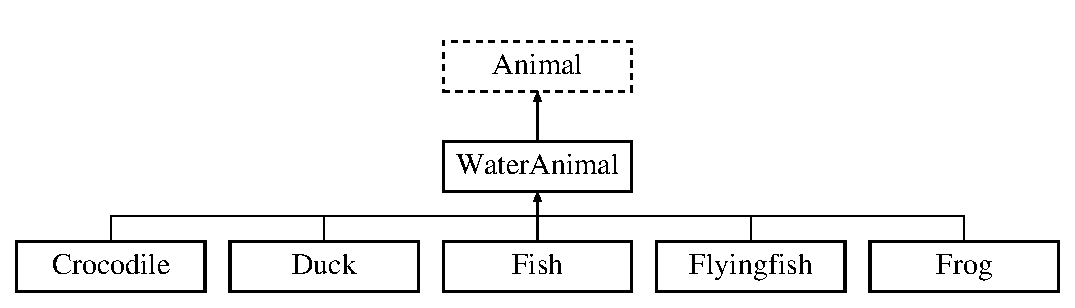
\includegraphics[height=3.000000cm]{classWaterAnimal}
\end{center}
\end{figure}
\subsection*{Public Member Functions}
\begin{DoxyCompactItemize}
\item 
\hypertarget{classWaterAnimal_a23d00047948b4b37186540ceb6d73559}{{\bfseries Water\-Animal} (int, int)}\label{classWaterAnimal_a23d00047948b4b37186540ceb6d73559}

\item 
\hypertarget{classWaterAnimal_a6b05aefda40def7833a1e8556faefbe2}{{\bfseries Water\-Animal} (const \hyperlink{classWaterAnimal}{Water\-Animal} \&)}\label{classWaterAnimal_a6b05aefda40def7833a1e8556faefbe2}

\item 
\hypertarget{classWaterAnimal_a69b278c7cf7c9095461c4e428e4b3c52}{virtual string {\bfseries interact} ()=0}\label{classWaterAnimal_a69b278c7cf7c9095461c4e428e4b3c52}

\item 
\hypertarget{classWaterAnimal_aa9c9c82092a8c7d248d2a96c2ea15073}{virtual string {\bfseries get\-Tipe\-Habitat} ()}\label{classWaterAnimal_aa9c9c82092a8c7d248d2a96c2ea15073}

\item 
\hypertarget{classWaterAnimal_ad64d5de05465a6cbd11fd2d83d507f74}{virtual string {\bfseries get\-Tipe\-Animal} ()=0}\label{classWaterAnimal_ad64d5de05465a6cbd11fd2d83d507f74}

\end{DoxyCompactItemize}
\subsection*{Protected Attributes}
\begin{DoxyCompactItemize}
\item 
\hypertarget{classWaterAnimal_af8fd1fd731bd336dbe1133d0e950004a}{const string {\bfseries tipe\-Habitat} = \char`\"{}water\char`\"{}}\label{classWaterAnimal_af8fd1fd731bd336dbe1133d0e950004a}

\end{DoxyCompactItemize}


The documentation for this class was generated from the following files\-:\begin{DoxyCompactItemize}
\item 
Water\-Animal.\-h\item 
Water\-Animal.\-cpp\end{DoxyCompactItemize}

\hypertarget{classWaterHabitat}{\section{Water\-Habitat Class Reference}
\label{classWaterHabitat}\index{Water\-Habitat@{Water\-Habitat}}
}


{\ttfamily \#include $<$Air\-Habitat.\-h$>$}

Inheritance diagram for Water\-Habitat\-:\begin{figure}[H]
\begin{center}
\leavevmode
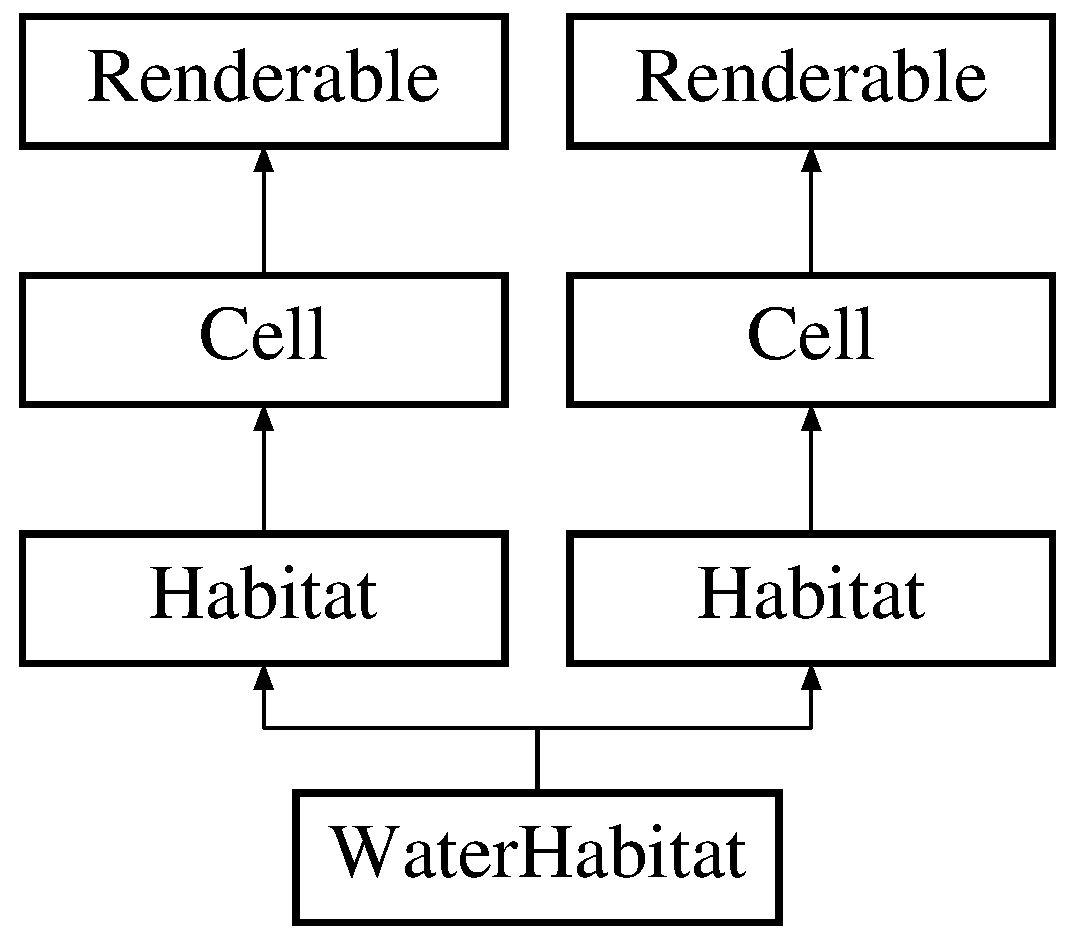
\includegraphics[height=4.000000cm]{classWaterHabitat}
\end{center}
\end{figure}
\subsection*{Public Member Functions}
\begin{DoxyCompactItemize}
\item 
\hyperlink{classWaterHabitat_a0e4b21bb7912f199945b5533457dbdcf}{Water\-Habitat} (int x, int y, char s)
\begin{DoxyCompactList}\small\item\em Constructor. \end{DoxyCompactList}\item 
string \hyperlink{classWaterHabitat_a02b4e524ab689f2e2b54b74acb58f7b2}{get\-Tipe} ()
\begin{DoxyCompactList}\small\item\em Mendapatkan tipe \hyperlink{classCell}{Cell}. \end{DoxyCompactList}\item 
\hyperlink{classWaterHabitat_a0e4b21bb7912f199945b5533457dbdcf}{Water\-Habitat} (int x, int y, char s)
\begin{DoxyCompactList}\small\item\em Constructor. \end{DoxyCompactList}\item 
string \hyperlink{classWaterHabitat_a02b4e524ab689f2e2b54b74acb58f7b2}{get\-Tipe} ()
\begin{DoxyCompactList}\small\item\em Mendapatkan tipe \hyperlink{classCell}{Cell}. \end{DoxyCompactList}\end{DoxyCompactItemize}


\subsection{Detailed Description}
Kelas \hyperlink{classWaterHabitat}{Water\-Habitat} adalah kelas turunan dari \hyperlink{classHabitat}{Habitat} 

\subsection{Constructor \& Destructor Documentation}
\hypertarget{classWaterHabitat_a0e4b21bb7912f199945b5533457dbdcf}{\index{Water\-Habitat@{Water\-Habitat}!Water\-Habitat@{Water\-Habitat}}
\index{Water\-Habitat@{Water\-Habitat}!WaterHabitat@{Water\-Habitat}}
\subsubsection[{Water\-Habitat}]{\setlength{\rightskip}{0pt plus 5cm}Water\-Habitat\-::\-Water\-Habitat (
\begin{DoxyParamCaption}
\item[{int}]{x, }
\item[{int}]{y, }
\item[{char}]{s}
\end{DoxyParamCaption}
)}}\label{classWaterHabitat_a0e4b21bb7912f199945b5533457dbdcf}


Constructor. 


\begin{DoxyParams}{Parameters}
{\em x} & Indeks baris \\
\hline
{\em y} & Indeks kolom \\
\hline
{\em s} & Simbol \\
\hline
\end{DoxyParams}
\hypertarget{classWaterHabitat_a0e4b21bb7912f199945b5533457dbdcf}{\index{Water\-Habitat@{Water\-Habitat}!Water\-Habitat@{Water\-Habitat}}
\index{Water\-Habitat@{Water\-Habitat}!WaterHabitat@{Water\-Habitat}}
\subsubsection[{Water\-Habitat}]{\setlength{\rightskip}{0pt plus 5cm}Water\-Habitat\-::\-Water\-Habitat (
\begin{DoxyParamCaption}
\item[{int}]{x, }
\item[{int}]{y, }
\item[{char}]{s}
\end{DoxyParamCaption}
)}}\label{classWaterHabitat_a0e4b21bb7912f199945b5533457dbdcf}


Constructor. 


\begin{DoxyParams}{Parameters}
{\em x} & Indeks baris \\
\hline
{\em y} & Indeks kolom \\
\hline
{\em s} & Simbol \\
\hline
\end{DoxyParams}


\subsection{Member Function Documentation}
\hypertarget{classWaterHabitat_a02b4e524ab689f2e2b54b74acb58f7b2}{\index{Water\-Habitat@{Water\-Habitat}!get\-Tipe@{get\-Tipe}}
\index{get\-Tipe@{get\-Tipe}!WaterHabitat@{Water\-Habitat}}
\subsubsection[{get\-Tipe}]{\setlength{\rightskip}{0pt plus 5cm}string Water\-Habitat\-::get\-Tipe (
\begin{DoxyParamCaption}
{}
\end{DoxyParamCaption}
)\hspace{0.3cm}{\ttfamily [virtual]}}}\label{classWaterHabitat_a02b4e524ab689f2e2b54b74acb58f7b2}


Mendapatkan tipe \hyperlink{classCell}{Cell}. 

\begin{DoxyReturn}{Returns}
tipe 
\end{DoxyReturn}


Implements \hyperlink{classHabitat_a4c8164f06a0a32ca6c7f465380b31ac0}{Habitat}.

\hypertarget{classWaterHabitat_a02b4e524ab689f2e2b54b74acb58f7b2}{\index{Water\-Habitat@{Water\-Habitat}!get\-Tipe@{get\-Tipe}}
\index{get\-Tipe@{get\-Tipe}!WaterHabitat@{Water\-Habitat}}
\subsubsection[{get\-Tipe}]{\setlength{\rightskip}{0pt plus 5cm}string Water\-Habitat\-::get\-Tipe (
\begin{DoxyParamCaption}
{}
\end{DoxyParamCaption}
)\hspace{0.3cm}{\ttfamily [virtual]}}}\label{classWaterHabitat_a02b4e524ab689f2e2b54b74acb58f7b2}


Mendapatkan tipe \hyperlink{classCell}{Cell}. 

\begin{DoxyReturn}{Returns}
tipe 
\end{DoxyReturn}


Implements \hyperlink{classHabitat_a4c8164f06a0a32ca6c7f465380b31ac0}{Habitat}.



The documentation for this class was generated from the following files\-:\begin{DoxyCompactItemize}
\item 
Air\-Habitat.\-h\item 
Water\-Habitat.\-h\item 
Water\-Habitat.\-cpp\end{DoxyCompactItemize}

%--- End generated contents ---

% Index
\newpage
\phantomsection
\addcontentsline{toc}{chapter}{Index}
\printindex

\end{document}
